\documentclass[11pt]{article}
\usepackage{geometry}
\geometry{verbose,tmargin=1in,bmargin=1in,lmargin=1.05in,rmargin=1.05in}  
\usepackage{setspace}
\makeatletter
\renewcommand\paragraph{\@startsection{paragraph}{4}{\z@}%
  {3.25ex \@plus 1ex \@minus .2ex}%  % space above the heading
  {1.5ex \@plus .2ex}%                  % space below (positive = display)
  {\normalfont\normalsize\bfseries}}
\makeatother     
\usepackage{enumitem}
\usepackage{fancyhdr}              
\usepackage{amsmath, amssymb, graphicx, hyperref}
\usepackage{amsmath, amsthm, amssymb}
\newtheorem{proposition}{Proposition}
\newtheorem{lemma}{Lemma}
\newtheorem{corollary}{Corollary}
\newtheorem{remark}{Remark}
\usepackage{float}
\newsavebox{\tabbox}
\usepackage{booktabs}
\usepackage{caption}    
\usepackage{subcaption}
\usepackage{natbib}
\usepackage{rotating}
\usepackage[T1]{fontenc}
\usepackage[utf8]{inputenc}
\usepackage{newtxtext}
\usepackage{newtxmath}

\title{\textbf{Integrate To Not Surrender: Roads, Trade and Urbanization in Brazil}}
\author{Jianing Shao \footnotemark}

\begin{document}

\onehalfspacing
\renewcommand{\thefootnote}{\fnsymbol{footnote}}
\maketitle
\begin{abstract}
This paper examines the impact of improvement in world market access on urbanization and agricultural specialization. I employ a 2SLS framework, utilizing the predicted road network from the Plan for National Integration (PIN) devised during the military dictatorship as a source of exogenous variation. The findings confirm a larger increase in urbanization level and specialization in transport-cost-sensitive agricultural commodities for micro-regions with larger reductions in travel time to the world market. A 10\% larger reduction in travel time raises urban population by 3.3\% and land in transport-cost-sensitive crops by 37\%, changes that operate mainly through the composition of population and of cultivated land. Event study estimates show the significant land-use response emerging after trade liberalization rather than immediately upon road construction. The gains are larger in micro-regions farther from their state capital, where new infrastructure is more valuable. These results are in line with the predictions of a Ricardian trade model, providing empirical evidence for a spatial Balassa-Samuelson mechanism that the increase in the tradable (rural) sector productivity translates into a growth in the non-tradable (urban) sector.
\end{abstract}

\footnotetext[1]{I am immensely grateful to my supervisor Prof. Daniel Sturm for providing invaluable support to guide this thesis throughout the academic year, Dr. Matthew Levy and my fellow BSc Econometrics and Mathematical Economics students for their inspiring questions and ideas discussed during the work-in-progress seminars. I also thank the 24th Carroll Round Conference committee and participants, especially Marco Uustal, for their useful comments. All errors are my own.}

\newpage

\renewcommand{\thefootnote}{\arabic{footnote}}

%TC:endignore

\section{Introduction}

The relationship between economic growth and trade is central to the fields of both international and development economics. A well-connected road network is essential for fostering both domestic and international trade. However, many rapidly developing countries, such as India, China, and Brazil, face significant constraints on their transportation infrastructure. To what extent do trade cost reductions brought by road construction promote urbanization and economic development? What are the distributional effects of international trade shocks? What role do internal trade costs play in the transmission of the shocks?

This paper seeks to provide new reduced-form evidence to answer these questions, using Brazil's substantial variation in internal integration following the Plan for National Integration (PIN) in 1970 as a natural experiment. The project called for the construction of nearly 20,000 km of highways to assert control over the Amazon. This empirical setting has several desirable features for examining the relationship between economic development and international trade. First, Brazil's integration into the world economy was fueled by the trade cost reductions induced by PIN. Implemented during Brazil's military dictatorship 20 years before the trade liberalization in 1990, this plan aimed to strengthen national security and hence is plausibly exogenous to the economic characteristics of Brazil's peripheral locations. Second, the expansion of the actual road network from 1970 to 2010 substantially lowered inland transport costs, especially for the previously underdeveloped Amazon, allowing for an examination of the role of internal integration in shaping development patterns. Third, the availability of disaggregated data on economic activities across regions in Brazil over 40 years enables the quantification of the structural transformation and expansion pattern of tradable commodities.

To address concerns about nonrandom road placement, I exploit the transport cost reductions induced by the PIN road network as an instrument for the actual reduction. I construct a decadal panel dataset from 1970 to 2010, combining micro-region-level characteristics, travel time to the closest international port on the actual road network, and outcome variables including GDP, population, urban population, the urban employment share, and agricultural land use and production. The data are also collapsed into a cross-section of changes in outcomes and in travel time between 1970 and 2010.

To guide the empirical investigation, I adapt a Ricardian trade model from Fajgelbaum and Redding (2022), which formalizes the role of transport costs in shaping the growth and distribution of economic activities across locations. The model has two central predictions for the impact of transport costs. First, it establishes a spatial Balassa-Samuelson effect linking structural transformation, economic development and international trade: locations with larger reductions in trade costs will see larger growth in GDP, population and urbanization. Second, locations with larger reductions in transport costs will specialize more in transport-cost-sensitive commodities. A third result characterizes when internal and external integration interact, and frames the interpretation of the timing rather than delivering a further tested prediction.

I find strong empirical support for these predictions. My baseline specification is a long-differenced estimation that controls for long-run trends during the 1970-2010 period. Using my newly constructed spatially disaggregated dataset, I find that over the 40-year period, locations with 10\% larger reductions in transport costs to world markets have a 3.3\% larger increase in urban population, a change that operates mainly through the composition of the population rather than its size. I further examine the time-varying effects of the reduction in travel time on outcomes of interest in an event study design. Dynamic estimates confirm that there are no pre-trends in urban population growth but a sudden spike from 1980 onwards for those micro-regions predicted to experience larger reductions in travel time to ports.

Turning to the composition of agricultural production, locations with 10\% larger reductions in transport costs devote 37\% more land to transport-cost-sensitive crops, a reallocation within the cultivated area rather than a proportionate expansion of it. I employ a probability model to uncover the expansion pattern and confirm that part of this reallocation came through entry into sensitive crops in micro-regions that previously grew none. The same ordering appears in a crop-level specification that measures sensitivity continuously by value per tonne and identifies it within micro-regions, so the result does not depend on how crops are grouped. Unlike the urbanization response, this reallocation emerges mainly after the trade liberalization of the early 1990s rather than immediately upon road construction. Additional heterogeneity analysis reveals that the effect of transport cost reductions is more pronounced in micro-regions where the newly built infrastructure is particularly valuable, with the clearest evidence for micro-regions farther away from the state capital. The main results survive a battery of robustness checks, including alternative robust estimators and alternative specifications and sample choices.

This paper relates to several bodies of literature. First, it builds most directly on work in economic geography on market access, including Hanson (1996), Venables and Limão (2002), Redding and Sturm (2008), Allen and Arkolakis (2014), Coşar and Fajgelbaum (2016), Redding (2016), Sotelo (2020), Fajgelbaum and Redding (2022), and Morten and Oliveira (2024). I adapt the framework of Fajgelbaum and Redding (2022) to Brazil and let transport costs differ across agricultural goods, so that market access acts as a source of comparative advantage within agriculture as well as between sectors, and I introduce a border wedge that makes the trade regime an explicit parameter rather than a fixed background condition.

Second, a growing empirical literature has examined the relationship between economic activity and transport infrastructure, including Chandra and Thompson (2000), Baum-Snow (2007), Michaels (2008), Berlinski, Galiani, and Jaitman (2011), Duranton and Turner (2012), Duranton, Morrow, and Turner (2014), Faber (2014), Atkin and Donaldson (2015), Coşar and Demir (2016), Storeygard (2016), Baum-Snow et al. (2017), Donaldson (2018), Pérez (2018), Banerjee, Duflo, and Qian (2020), and Heblich, Redding, and Sturm (2020), as reviewed in Redding and Turner (2015). Where this literature largely measures aggregate activity, I take the composition of agricultural land as an outcome, which tests the good-specific structure of the model directly.

Third, a rich set of spatial literature on the pattern of migration assumed that workers are immobile across space (Donaldson, 2018; Topalova, 2010), or that migration costs are purely due to preferences without frictions (Allen and Arkolakis, 2014; Redding, 2016). Recent literature relaxes these assumptions to consider costly migration (Tombe and Zhu, 2019; Morten and Oliveira, 2024). I model imperfect labor mobility through idiosyncratic location preferences, so that population responds to spatial real-income differences with a finite migration elasticity. In the data that response is compositional: the urban share rises while total population does not.

Last, I build on the economic and historical literature on Brazil's economic development, including Bird and Straub (2014), Pellegrina (2014), Pellegrina and Sotelo (2021), Pellegrina (2022), and Soled et al. (2024). This paper investigates the role of road access in promoting agricultural production and urbanization through the lens of trade, with a specific focus on the production of disaggregated agricultural commodities in Brazil.

The remainder of the paper is organized as follows. Section 2 discusses the historical background in Brazil between 1970 and 2010. Section 3 develops the theoretical model and derives the two key empirical predictions. Sections 4 and 5 discuss the data and identification strategy. Section 6 presents the main empirical results. Section 7 performs several robustness checks to validate the results. Section 8 interprets the results based on the theoretical model and discusses potential concerns. Section 9 concludes.

\section{Historical Context}
\subsection{Plan for National Integration (1970)}
The Legal Amazon, designated in 1948, comprises all seven states in Brazil’s North Region, most of Mato Grosso, and part of Maranhão. In 2010, the region accounted for about 10\% of the population and 8.1\% of GDP (IBGE, 2010). However, for most of the 20th century, the region was largely unoccupied and sparsely populated. Before the 1970s, the main transportation in the region was carried through the waterways with minimal road connection in between. 

Brazil began building transport infrastructure sporadically in the late nineteenth century. In 1964, Brazil became a military dictatorship. The valorization of the country's territorial attributes was accompanied by an increase in its defensive capacity. The need for a more effective occupation of the Amazon Rainforest was prioritized. One of the most decisive infrastructure construction projects was the Plan for National Integration (PIN) launched in 1970, which called for the construction of nearly 20,000 km of highway systems, including the Trans-Amazonia Highway, Cuiaba-Santarem Highway, and Northern Perimeter Highway with a network of feeder roads. Under the slogan “integrate to not surrender,” the government urged placing the stamp of Brazilian settlement on Amazonia so that Brazilian sovereignty would never be contested (Fearnside, 1984). The goal of PIN was twofold: firstly, to connect state capitals in the Legal Amazon with other regions in Brazil to assert control over the Amazon and thereby strengthen national sovereignty; secondly, to reduce the flux of migrants to the populated coastal metropolises. PIN established the objectives and identified the trunk highways. Their alignments were subsequently recorded in the \emph{Plano Nacional de Viação} (PNV), the statutory register of Brazil’s federal transport network. The 1973 revision of the PNV incorporated the PIN corridors as planned federal routes and therefore provides the cartographic record of the network that PIN intended to construct. The instrument described in Section \ref{sec:instrument} is georeferenced from this document, which is reproduced in Figure \ref{fig:pnv}.

Construction was only partially completed. By 1974, with rising social conflict and limited capacity, the PIN plan was canceled. Despite this, much of Brazil’s current freight movement—about 60\%—relies on infrastructure built during this era (Bottasso et al., 2021). PNV 1973 provided rights-of-way facilitating lower-cost highway construction or pavement over or alongside old roads, most of which has taken place since 1990. This gap between the planned and the realized network is what the empirical strategy exploits: the PNV alignments were fixed by the 1973 plan, whereas which of them were built, and when, depended on conditions that came later.

\subsection{Trade Liberalization (1990s)}
Brazil was heavily protected and imposed trade restrictions to address balance of payment difficulties despite being one of the founding members of the General Agreement on Tariffs and Trade. After the transition from a military to a civilian government in 1985, Brazil embarked on a major trade liberalization process driven by the macroeconomic and debt crises in many Latin American economies during the 1980s.

The trade reform broke the nearly 100-year-high barriers to trade. The average nominal tariffs were unilaterally lowered from 54.9\% in 1987 to 10.5\% in 1994. During the 1988-1989 period, tariff redundancy, special regimes, and additional taxes were partially removed. In March 1990, the newly elected president unexpectedly eliminated non-tariff trade barriers, and the trade liberalization effectively started. The trade reform in tariffs culminated in 1995 with the establishment of Mercosur, a multilateral common market to promote the free movement of goods, services, and productive factors between countries.

In July of 1994, the Brazilian government implemented a new macroeconomic stabilization plan called Plano Real to curb inflation. A prominent feature was the adoption of a crawling-peg exchange rate system in order to restore the public's confidence in the domestic currency. This plan was not successful in keeping government budget deficits under control and undermined the government's ability to sustain the crawling-peg system. In January of 1999, an unexpected and large speculative attack on the domestic currency left the Brazilian government with no other choice than to abandon the crawling peg and adopt a free-floating exchange rate system. A large real exchange rate devaluation of approximately 50\% then ensued, which, however, proves to further heighten incentives for farmers to increase their output of internationally traded commodities with prices in Brazilian reais approaching historical heights (Richards et al., 2012). This further boosted exports and incentivized agricultural expansion and investment in the region.

\subsection{Agriculture to Growth}
\label{sec:agtogrowth}
Brazil has emerged as a top global exporter of numerous agricultural products. Soybeans have been pivotal in the growth of Brazil's agricultural sector and its rise as a leading global agricultural exporter. Commercial soybean cultivation began in the 1940s and was solidified in the southern states during the 1960s, aided by industrial support under the military regime indirectly benefiting agricultural commodities.

Post-liberalization, the soybean complex spread to the Cerrado and Amazon, gradually replacing the South. By 2005, Mato Grosso had become the leading soybean-exporting state. Such conversion of previous range, pasture, and uncultivated land into cropland was driven by both rising international demand and supply factors: technological development, which made feasible the cultivation in formerly inhospitable areas, and the investment in infrastructure, which greatly reduced transportation costs (Mueller, 2003).

Such supply-side drivers laid the groundwork for the agricultural establishment in the West. First, the National Agricultural Research Institution developed new seed varieties that thrived under the diverse and challenging tropical conditions, making previously unsuitable low-latitude areas viable for soybean cultivation. Second, paving of previously constructed PIN highways, such as the Cuiaba-Santarem Highway, has substantially enhanced connectivity by linking the Cerrado directly to the ports along the Amazon River in Santarém, which offers a logistical advantage for the region’s substantial agricultural outputs over the distant Port of Santos. The improvement in infrastructure has dramatically reduced travel times during the rainy season from weeks to hours, improving market access and accommodating the growing demand for soybeans.

These two supply-side forces are entangled, and the design that follows does not fully separate them. The estimates remove what operates at the level of a location, but not a shock specific to a single crop, and the cultivar breakthrough was one: it transformed soybeans, which are also the most transport-cost-sensitive crop in the sample. Section \ref{sec:link} argues that within the model the two are complementary rather than rival forces, and Section \ref{sec:concerns} explains why no specification available in this setting can tell them apart. 

\subsection{Spatial Pattern of Economic Development}
Reflecting the pattern of road connection, the spatial distribution of economic activity within Brazil was highly unequal. In 1970, Brazil’s economic activity was concentrated in coastal cities, which generated over 70\% of GDP. 
Table \ref{tab:descriptives} shows a strong correlation between proximity to ports and economic outcomes using the baseline specification
\begin{equation}
    \log Y_{is} = a+b \log(\text{Travel Time})_{is}+u_{is}
\end{equation}
where $i$ indexes micro-regions and $\log(\text{Travel Time})_{is}$ is a measure of geographical access to world markets using travel time to the closest port, and $u_{is}$ is a stochastic error. \footnote{Both sides enter in logs, so $b$ is an elasticity, in the same units as the treatment used from Section 5 onwards. }

Table \ref{tab:descriptives} reports the estimated elasticities. Locations close to world markets have not only higher GDP and population but also higher urbanization levels. Within agriculture the pattern is more selective. Coffee, Brazil's established export crop, is strongly concentrated in micro-regions closer to ports. Neither soybean nor cattle shows a gradient. For soybean this reflects the timing described above: in 1974 the complex was still confined to the southern states, as yet untouched by the Cerrado expansion that came after liberalization, so the cross-section predates the reallocation this paper studies. Cattle is raised predominantly for the domestic market and delivered to slaughterhouses rather than to ports even when exported, so its location need not track distance to the gateway. Cross-sectional crop location therefore reveals little about transport costs, which is why the empirical analysis identifies from changes in travel time rather than from levels.

\section{Theoretical Model}

In this section, I adapt the theoretical model from Fajgelbaum and Redding (2022) into the Brazilian setting. The model is developed based on a Ricardian Trade model (Eaton and Kortum, 2002) to capture the distribution of economic activities within Brazil across sectors and locations.
The purpose of this section is not to provide a full structural quantitative framework, but rather to derive two key empirical predictions to guide the empirical analysis: first, locations with larger reductions in internal trade costs to world markets experience greater structural transformation toward non-tradable activity; second, such locations specialize in transport-cost-sensitive agricultural goods. A final result characterizes when internal and external integration interact, and serves to frame the interpretation of the post-liberalization timing rather than to deliver a third tested prediction. All detailed derivations and proofs are collected in Appendix \ref{app:derivations}.

Consider a small open economy with a set of locations $\ell \in L$. Each location is endowed with a fixed amount of land $L_\ell$ and a mobile labor force. There are three sectors: agriculture ($A$), manufacturing ($M$), and non-tradables ($N$). Agriculture and manufacturing are tradable, and non-tradables are locally consumed. Within agriculture, there is a set of disaggregated agricultural goods indexed by $g = 1,\dots,G$ to account for the observed differences in the composition of agricultural production across locations. Each location's land consists of a continuum of land plots $j\in[0,L_{\ell}]$ that are heterogeneous in productivity for disaggregated agricultural goods $g=1,..., G$. 

Each location is connected through an internal road network to international markets, and transport costs change over time as that network expands. Let $\delta_{g(\ell,\ell^*)}=e^{\tau_g t_\ell}\geq 1$ denote the iceberg transport cost between location $\ell$ and the closest international gateway $\ell^*$ for good $g$: shipping one unit between $\ell$ and $\ell^*$ delivers $1/\delta_{g(\ell,\ell^*)}$ units, where $\tau_g>0$ is the heterogeneous transport-cost sensitivity for each good and $t_\ell$ is the common travel time term from location $\ell$ to the closest international port. The transport cost for manufactures is defined analogously as $\delta_{M(\ell,\ell^*)}=e^{\tau_M t_\ell}$ with $\tau_M>0$. I abstract from internal bilateral trade in disaggregated agricultural goods and focus on the case in which local prices are ultimately pinned down through no-arbitrage by exogenous world prices at the closest international gateway ($\{P_g^\ast\}_{g=1}^{G}, P_M^\ast$) and internal transport costs.

\paragraph{A. Preferences}
Workers' preferences $b_\ell u_\ell$ for each location consist of a common component $u_\ell$ that is the same for all workers and an idiosyncratic component $b_\ell$. The common component has two tiers: Workers consume tradable and non-tradable goods with constant elasticity of substitution (CES) preferences
\begin{equation}
    u_{\ell} = \left[ \beta_T^{\frac{1}{\sigma}} C_{T\ell}^{\frac{\sigma-1}{\sigma}} + (1 - \beta_T)^{\frac{1}{\sigma}} C_{N\ell}^{\frac{\sigma-1}{\sigma}} \right]^{\frac{\sigma}{\sigma-1}},
    \qquad 0<\sigma<1.
\label{eq:utility}
\end{equation}
where $\beta_T \in (0,1)$ controls the relative weights of tradable and non-tradable goods. I assume inelastic demand between sectors as in the macroeconomics literature on structural transformation. 

Tradables consumption is defined over the manufacturing good and the set of disaggregated agricultural goods with Cobb-Douglas preferences:
\begin{equation}
    C_{T\ell}= C_{M\ell}^{\,1-\gamma_A}\prod_{g=1}^G C_{g\ell}^{\gamma_g},
    \qquad
    \sum_{g=1}^G \gamma_g = \gamma_A \in (0,1),
    \label{eq:tradables_nest}
\end{equation}
where $\gamma_g$ is the expenditure share of agricultural good $g$ within tradables and $\gamma_A$ is the total agricultural expenditure share within tradables. The corresponding tradables price index is, up to a multiplicative constant,
\begin{equation}
        E_{T\ell}= P_{M\ell}^{\,1-\gamma_A}\prod_{g=1}^G P_{g\ell}^{\gamma_g}.
    \label{eq:ET}
\end{equation}
 
The idiosyncratic component $b_\ell$ captures heterogeneity in workers' tastes for locations drawn independently from a Fréchet distribution with shape parameter $\epsilon$ \footnote{The scale parameter is normalized to 1 for all locations.}:
\begin{equation}
    \text{Pr}[b_{\ell}<b] = \exp(-b^{-\epsilon}), \qquad \epsilon>0
\end{equation}

Workers observe their idiosyncratic tastes for each location and choose where to live by maximizing utility. Given that the maximum of Fréchet random variables is also Fréchet distributed, the probability of choosing location $\ell$ equals $u_\ell^\epsilon/\sum_{k \in L} u_k^\epsilon$, so conditional on the exogenous total supply of labor $N$, labor allocated to location $\ell$ is
\begin{equation}
N_\ell = n_\ell L_\ell = N \left(\frac{u_\ell}{u^*}\right)^{\epsilon},
\qquad
u^* = \left( \sum_{k \in L} u_k^\epsilon \right)^{1/\epsilon},
\label{eq:density_supply}
\end{equation}
where $n_\ell \equiv N_\ell/L_\ell$ is population density and $u^*$ is proportional to workers' expected utility, $\mathbb{E}[\max_\ell b_\ell u_\ell]=\Gamma(1-1/\epsilon)\,u^*$, which is finite given $\epsilon>1$. A larger shape parameter $\epsilon$ implies greater internal labor mobility: the supply of labor to each location is more responsive to relative utility levels.

\paragraph{B. Production}
Each worker is endowed with one unit of labor supplied inelastically with zero disutility. Land is owned by immobile landowners who do not own any labor. Production in each sector is characterized by a Cobb-Douglas technology with constant returns to scale in land and labor. Output per unit of land in non-tradable and for an agricultural good $g$ in land plot $j$ in location $\ell$ are
\begin{align}
    q_{N\ell} = z_{N\ell} n_{N\ell}^{1-\alpha_N}, \quad
    q_{M\ell} = z_{M\ell} n_{M\ell}^{1-\alpha_M}, \quad
    q_{g\ell j} = z_{g\ell j} n_{g\ell j}^{1-\alpha_A},
\end{align}
where $z_{N\ell},z_{M\ell}, z_{g\ell j}$ are sectoral productivities and $0<\alpha_i<1$ is the land intensity in sector $i=A, M, N$. Following Fajgelbaum and Redding (2022), I assume $\alpha_N<\alpha_M<\alpha_A$, so agriculture is the most land-intensive sector and non-tradables the least.

Land plots differ in productivity for disaggregated agricultural goods drawn from the following Fr\'echet distribution with a shape parameter $\theta$ \footnote{Note that this Fr\'echet distribution has a different shape parameter than the distribution of idiosyncratic taste.}:
\begin{equation}
\Pr\!\left[z_{g\ell j}\le z\right]
=
\exp\!\left(-T_{g\ell}\, z^{-\theta}\right),
\qquad \theta>0,
\label{eq:frechet_prod}
\end{equation}
where $T_{g\ell}$ captures location-specific comparative advantage in good $g$.

Production in each sector is perfectly competitive. Producers choose employment density to maximize profits, taking the prices of goods and input factors as given. In equilibrium, firms make zero profits in each sector and location with positive production. If a land plot is used for manufacturing or non-tradables, land rents are equal to revenue per unit of land minus labor costs per unit of land at the equilibrium of employment density: 
\begin{equation}
    r_{i\ell} = \max_{n_{i\ell}} \{ P_{i\ell} q_i (n_{i\ell}) - w_\ell n_{i\ell} \}, \quad  i \in  \{M, N\}
\end{equation}
If a land plot is used in agriculture, it is allocated to the agricultural good with the highest rent
\begin{equation}
    r_{\ell j} = \max_{g=1, \ldots, G} \{r_{g\ell j}\}, \quad
    r_{g\ell j} = \max_{n_{g\ell j}} \left( P_{g\ell} q_{g\ell} (n_{g\ell j}) - w_{\ell} n_{g\ell j} \right).
\label{eq:landalloc}
\end{equation}
Hence, the land-allocation decision depends on land rents in the manufacturing and non-tradable sectors ($r_{M\ell}$, $r_{N\ell}$) and expected land rents in agriculture ($r_{A\ell}=\mathbb{E}[r_{\ell j}]$), and if a land plot has been allocated to agriculture, the landowner observes the realizations for productivity of each good and decides which good to produce.

Before deriving the equilibrium wage-rental ratio, I first establish an aggregate measure of agricultural revenue productivity ($z_{A\ell}$). Under equation \eqref{eq:frechet_prod}, there exists a sufficient statistic for the disaggregated agricultural goods on aggregate employment and output in agriculture (see derivations in Appendix \ref{app:zA}):
\begin{equation}
z_{A\ell}
=
\Gamma\!\left(\frac{\alpha_A\theta-1}{\alpha_A\theta}\right)^{\alpha_A}
\left[
\sum_{g=1}^G T_{g\ell} P_{g\ell}^\theta
\right]^{\frac{1}{\theta}}, \qquad \alpha_A\theta>1
\label{eq:zA}
\end{equation}

The same Fréchet structure pins down the allocation of agricultural land across goods: with a continuum of plots, the share of agricultural land in location $\ell$ allocated to good $g$ equals the probability that an individual plot obtains its highest rent from good $g$, which by \eqref{eq:frechet_prod} and the rent-maximization problem \eqref{eq:landalloc} is
\begin{equation}
l_{g\ell}
=
\frac{T_{g\ell}P_{g\ell}^\theta}
{\sum_{h=1}^G T_{h\ell}P_{h\ell}^\theta}.
\label{eq:landshare}
\end{equation}
Log-differentiating equation \eqref{eq:zA} shows that the land shares are also the elasticities of aggregate revenue productivity with respect to the disaggregated prices, $\partial \ln z_{A\ell}/\partial \ln P_{g\ell} = l_{g\ell}$.

Land shares in \eqref{eq:landshare} are strictly positive for every good with $T_{g\ell}>0$, so the model itself contains no discrete margin at which a good starts or ceases to be produced. Observed production, however, is recorded only above a reporting threshold. I therefore let a good be \emph{observed} in location $\ell$ when its land share exceeds a minimum viable level, $l_{g\ell}\geq\varepsilon$ for some $\varepsilon>0$, which may be motivated by a minimum shipment size below which no trader serves the location. The threshold leaves every equilibrium object unchanged and affects only the mapping from the model to observed production.

Define adjusted agricultural productivity as
\begin{equation}
\tilde z_{A\ell} \equiv \frac{z_{A\ell}}{E_{T\ell}},
\label{eq:zad}
\end{equation}
where $E_{T\ell}$ is the tradables price index in \eqref{eq:ET}.

\paragraph{C. Wage-Rental Ratio}
Let the wage-rental ratio in sector $i$ and location $\ell$ be $\omega_{i\ell} \equiv w_\ell / r_{i\ell}$. Using profit maximization and the zero-profit condition, employment density in any active sector can be written in terms of the equilibrium wage-rental ratio by deriving the marginal product of labor and land
\begin{equation}
    n_{i\ell}=\frac{1-\alpha_i}{\alpha_i}\frac{1}{\omega_{i\ell}}
    \label{eq:n}
\end{equation}
and the sectoral wage-rental ratio is
\begin{equation}
    \omega_{i\ell}=(\frac{w_\ell}{P_{i\ell}z_{i\ell}})^\frac{1}{\alpha_i}
    \label{eq:omega}
\end{equation}

For agriculture, the aggregation result in equation~\eqref{eq:zA} implies
that the sector can be treated as a single-good sector with common
revenue productivity $z_{A\ell}$. Thus, employment density ($n_{A\ell}$) and the wage-rental ratio ($\omega_{A\ell}$) take the same form as equations \eqref{eq:n} and \eqref{eq:omega} but using the expected land rent $r_{A\ell}=\mathbb{E}[r_{\ell j}]$ and replacing $P_{i\ell}z_{i\ell}$ with aggregate revenue productivity ($z_{A\ell}$).

\paragraph{D. General Equilibrium Definition}
Given the exogenous total population $N$, a general equilibrium consists of expected utility $u^\ast$, allocations of population density $n_\ell$, land $\{L_{i\ell}\}_{i=A,M,N}$, and employment density $\{n_{i\ell}\}_{i=A,M,N}$, wages $w_\ell$, land rents $r_\ell$, and prices $\{P_{g\ell}\}_{g=1}^{G}$, $P_{M\ell}$, and $P_{N\ell}$ for all
$\ell \in L$, such that:
\begin{enumerate}[label=\roman*.]
    \item Workers maximize utility and choose their location optimally; $n_\ell L_\ell = \left(\frac{u_\ell}{u^*}\right)^\epsilon N$.
    \item Producers maximize profits and land is allocated optimally across sectors: $r_{\ell} = \max\{r_{A\ell}, r_{M\ell}, r_{N\ell}\}$.
    \item The land market clears in each location: $\sum_{i=A, M, N} L_{i\ell} = L_{\ell}$.
    \item The labor market clears in each location: $\sum_{i=A, M,  N} \left(\frac{L_{i\ell}}{L_{\ell}}\right) n_{i\ell} = n_{\ell}$.
    \item The non-tradables market clears in each location: $c_{N\ell} = (L_{N\ell}/L_{\ell}) q_{N} (n_{N\ell})$.
    \item Tradable goods prices are determined by no-arbitrage: if agricultural goods are exported and manufacturing goods are imported, $ P_{g\ell} = P_g^\ast / \delta_{g(\ell, \ell^\ast)}$ and $P_{M\ell} = P_M^\ast \delta_{M(\ell, \ell^\ast)}$.
\end{enumerate}

\paragraph{E. Local Equilibrium}
Whether a location is open to trade is determined by comparative advantage and transport costs: trade occurs when the relative price of imported manufactures net of transport costs falls below the autarky relative price, which for given transport costs happens when the location's comparative advantage in agriculture ($z_{A\ell}/z_{M\ell}$) is large enough. Equation \eqref{eq:omega} shows that the wage-rental ratio consistent with zero profits in each traded sector depends only on the common wage, the sector's price and its productivity, and not on the scale of production in any sector. Therefore, one traded sector will in general have a strictly lower wage-rental ratio than the other, so a location that trades produces only one traded good. On the basis of the overwhelming concentration of Brazilian exports in agriculture, I assume that all populated locations have a large enough $z_{A\ell}/z_{M\ell}$ to be open to trade with complete specialization in agriculture. \footnote{At sufficiently high transport costs the model instead features a \emph{trade frontier}, beyond which locations produce manufactures locally and cease to import them. Coşar and Fajgelbaum (2016) study this property in a model without a non-tradable sector, and Fajgelbaum and Redding (2022) note it and likewise assume it away. The margin that defines the frontier is the manufacturing-import decision, and a location on either side of it may still export agricultural goods, so the composition of agricultural production carries no signature of the frontier's location.}

A location that trades therefore has two active sectors, agriculture and non-tradables \footnote{The non-tradable sector always operates because the CES preferences in \eqref{eq:utility} imply unbounded marginal utility as consumption of non-tradables approaches zero.}. Since land is allocated to the sector with the highest rent, both active sectors pay a common land rent $r_\ell$ in equilibrium. Let $\omega_\ell \equiv w_\ell/r_\ell$, $\lambda_{A\ell}$ and $\nu_{A\ell}$ denote the location-level wage-rental ratio,  agricultural land and labor share respectively. Under CES demand, the tradable expenditure share is
\begin{equation}
s_{T\ell}=\beta_T\left(\frac{E_{T\ell}}{E_\ell}\right)^{1-\sigma},
\label{eq:sT_def}
\end{equation}
where the overall consumption price index implied by the preferences in \eqref{eq:utility} is
\begin{equation}
E_\ell=\left[\beta_T E_{T\ell}^{1-\sigma}+\left(1-\beta_T\right)P_{N\ell}^{1-\sigma}\right]^{\frac{1}{1-\sigma}}.
\label{eq:E}
\end{equation}
Income per unit of land is the sum of labor and land income,
\begin{equation}
y_\ell = w_\ell n_\ell + r_\ell = w_\ell\left(n_\ell+\omega_\ell^{-1}\right).
\label{eq:income}
\end{equation}

Combining profit maximization with the land, labor, and non-tradable market clearing conditions yields closed-form solutions for population density and the agricultural labor share (see derivations in Appendix \ref{app:localeq}):
\begin{equation}
n_\ell
=
\left(
\frac{1}{\alpha_N + (\alpha_A-\alpha_N)s_{T\ell}} - 1
\right)
\frac{1}{\omega_\ell},
\label{eq:density}
\end{equation}
\begin{equation}
\nu_{A\ell}
=
\frac{(1-\alpha_A)s_{T\ell}}
{1-\alpha_N-(\alpha_A-\alpha_N)s_{T\ell}}.
\label{eq:nuA}
\end{equation}
Both closed forms are functions of the wage-rental ratio and the tradable expenditure share alone: population density is decreasing in $\omega_\ell$ and, given $\alpha_A>\alpha_N$, in $s_{T\ell}$, whereas the agricultural labor share is increasing in $s_{T\ell}$. Characterizing the response of structural transformation to market access therefore requires only the comparative statics of $\omega_\ell$ and $s_{T\ell}$ with respect to travel time. Using the zero-profit conditions in the two active sectors, factor prices satisfy
\begin{align}
w_\ell &= z_{A\ell}\,\omega_\ell^{\alpha_A},
\label{eq:wage}\\
r_\ell &= z_{A\ell}\,\omega_\ell^{\alpha_A-1},
\label{eq:rent}\\
P_{N\ell} &= \frac{z_{A\ell}}{z_{N\ell}}\,\omega_\ell^{\alpha_A-\alpha_N}.
\label{eq:PN}
\end{align}
Expressing the common component of utility in the indirect form $u_\ell=w_\ell/E_\ell$ and substituting the factor prices into the price index \eqref{eq:E} yields:
\begin{equation}
u_\ell
=
\left[
\beta_T \left(\tilde z_{A\ell}\,\omega_\ell^{\alpha_A}\right)^{\sigma-1}
+
\left(1-\beta_T\right)\left(z_{N\ell}\,\omega_\ell^{\alpha_N}\right)^{\sigma-1}
\right]^{\frac{1}{\sigma-1}}
\label{eq:omega_eq}
\end{equation}

With population mobile, all populated locations offer the same utility level, $u_\ell=u^\ast$. Since location characteristics then enter equation \eqref{eq:omega_eq} only through adjusted agricultural productivity ($\tilde z_{A\ell}$) and non-tradable productivity ($z_{N\ell}$), and the right-hand side is strictly increasing in $\omega_\ell$ when $\sigma<1$, the equation determines a unique wage-rental ratio $\omega_\ell$. That wage-rental ratio determines the tradable expenditure share (see derivations in Appendix \ref{app:suff}) and hence population density and the agricultural labor share in equations \eqref{eq:density} and \eqref{eq:nuA}. Conditional on $u^\ast$, the two productivities are therefore sufficient statistics for local equilibrium outcomes:
\begin{equation}
n_\ell=n\left(\tilde z_{A\ell},z_{N\ell}\right),
\qquad
\nu_{A\ell}=\nu_A\left(\tilde z_{A\ell},z_{N\ell}\right)
\label{eq:reduced_local}
\end{equation}

The model closes at the national level, where $u^\ast$ adjusts so that location populations sum to $N$.

With the local equilibrium characterized, the remainder of this section derives the model's two empirical predictions. The first concerns structural transformation. Since travel time affects local outcomes only through the sufficient statistic $\tilde z_{A\ell}$ in equation \eqref{eq:reduced_local}, the argument proceeds in two steps: Lemma \ref{lem:zad} establishes that better market access raises adjusted agricultural productivity, and Proposition \ref{prop:bs} characterizes how the local equilibrium responds to it.

\begin{lemma}[Trade costs and adjusted agricultural productivity]
\label{lem:zad}
Suppose location $\ell$ imports manufactures and its agricultural trade position satisfies
\begin{equation}
\sum_{g=1}^G \left(l_{g\ell}-\gamma_g\right)\tau_g + (1-\gamma_A)\tau_M \;>\; 0.
\label{eq:net_export}
\end{equation}
Then
\begin{equation}
\frac{d \ln \tilde z_{A\ell}}{d t_\ell}
= -\Big[\sum_{g=1}^G \left(l_{g\ell}-\gamma_g\right)\tau_g + (1-\gamma_A)\tau_M\Big] < 0,
\label{eq:zad_t}
\end{equation}
so a reduction in travel time strictly raises adjusted agricultural productivity.
\end{lemma}

\noindent\emph{Proof.} See Appendix \ref{app:proof_zad}.\medskip

Condition \eqref{eq:net_export} requires the location to be, on balance, a net seller of the transport-cost-sensitive goods. \footnote{The weight $l_{g\ell}-\gamma_g$ is the share of good $g$ in the location's agricultural revenue less its share in local tradable spending, and each is weighted by that good's transport-cost sensitivity $\tau_g$. Better market access raises the price of each good for local producers and local consumers alike, so for a good the location produces in the same proportion as it consumes the two effects cancel exactly and it contributes nothing to the derivative; only the gap between its production and consumption shares matters. Imported manufactures work unambiguously in favour, since they become cheaper as travel time falls, and that is the term $(1-\gamma_A)\tau_M$.} This is a weak requirement. Since $\sum_g l_{g\ell}=1$ while $\sum_g \gamma_g=\gamma_A<1$, the weights $l_{g\ell}-\gamma_g$ sum to $1-\gamma_A>0$, and the manufacturing term is positive \footnote{Because the location produces only agricultural tradables while spending a share $1-\gamma_A$ of its tradable budget on manufactures, the weights $l_{g\ell}-\gamma_g$ sum to $1-\gamma_A>0$: in aggregate it is necessarily a net seller of agriculture and a net buyer of manufactures. Within agriculture, however, a location may consume a larger share of some good than it produces, so that $l_{g\ell}<\gamma_g$ and it buys that good in.}, Condition \eqref{eq:net_export} fails only if those goods are disproportionately the transport-cost-sensitive ones, so that the rise in their local price outweighs the gain on what the location sells. The condition does not disturb the price structure, since no-arbitrage pins local prices to the gateway whether the location is a net seller or a net buyer of any particular good.

The second step characterizes the local equilibrium as a function of travel time. Throughout, locations are compared holding fixed world prices, the land productivities $T_{g\ell}$, non-tradable productivity $z_{N\ell}$, and economy-wide expected utility $u^\ast$, so that they differ only in travel time to the gateway. This is the spatial Balassa-Samuelson effect: an improvement in the revenue productivity of the traded sector reallocates the local economy toward the labor-intensive non-tradable sector.

\begin{proposition}[Spatial Balassa-Samuelson effect]
\label{prop:bs}
Assume agricultural and non-tradable goods are complements ($\sigma<1$), agriculture is land-intensive relative to non-tradables ($\alpha_A>\alpha_N$), population is mobile ($\epsilon$ sufficiently large), \footnote{Perfect mobility is stronger than necessary. Fajgelbaum and Redding (2022, Proposition 3) establish results (ii)-(iv) for any finite migration elasticity $\epsilon>0$; only the decline in the wage-rental ratio requires $\epsilon$ above a threshold, and under fully immobile labor $\omega_\ell$ instead rises. The sign of the density and employment-share predictions is therefore robust to limited migration, although their magnitude vanishes as $\epsilon\to 0$, while the direction of the factor-price response depends on the strength of labor mobility.} and condition \eqref{eq:net_export} holds. Then a location with lower travel time $t_\ell$ has (i) higher adjusted agricultural productivity $\tilde z_{A\ell}$; (ii) a lower tradable expenditure share $s_{T\ell}$; (iii) higher population density $n_\ell$; (iv) a lower agricultural employment share $\nu_{A\ell}$; (v) a lower wage-rental ratio $\omega_\ell$; and (vi) higher GDP per unit of land $y_\ell$ in equation \eqref{eq:income}.
\end{proposition}

\noindent\emph{Proof.} See Appendix \ref{app:proof_bs}.\medskip

The economic intuition is as follows. Better access to world markets raises profitability in the tradable rural sector, which increases income and attracts population. When population rises, the reward to immobile land increases relative to the reward to mobile labor. This induces either more labor-intensive techniques within sectors or a reallocation of labor toward the labor-intensive non-tradable sector. Hence, reductions in internal trade costs to world markets generate structural transformation from tradable rural activity toward non-tradable urban activity, given the inelastic demand between sectors.

This first prediction concerns aggregate outcomes within a location. A second prediction concerns the composition of agricultural production across the disaggregated goods: given transport costs are good-specific, market access is itself a source of comparative advantage within agriculture.

\begin{proposition}[Specialization within agriculture]
\label{prop:specialization}
Locations with shorter travel time to the international gateway allocate relatively more land to transport-cost-sensitive agricultural goods: for every good $g$,
\begin{equation}
    \frac{d \ln l_{g\ell}}{d t_\ell}
= -\theta \left(\tau_g - \bar{\tau}_\ell\right),
\qquad
\bar{\tau}_\ell \equiv \sum_{h=1}^G l_{h\ell} \tau_h,
\label{eq:landshare_d}
\end{equation}
where $\bar{\tau}_\ell$ is the land-share-weighted average transport-cost sensitivity in location $\ell$. As travel time falls, the land share rises for goods with above-average transport-cost sensitivity ($\tau_g > \bar{\tau}_\ell$) and falls for goods with below-average sensitivity.
\end{proposition}

\noindent\emph{Proof.} See Appendix \ref{app:proof_spec}.\medskip

Intuitively, transport-cost-insensitive goods face little penalty from being produced inland, whereas transport-cost-sensitive goods benefit disproportionately from improved access to ports. Therefore, locations with better export access will specialize in transport-cost-sensitive goods: for the same reduction in $t_\ell$, land shares grow faster for more transport-cost-sensitive goods.

Proposition \ref{prop:specialization} also has an implication for the set of goods observed under the reporting threshold introduced in Section 3.B. Since the shares of goods with $\tau_g>\bar\tau_\ell$ fall fastest as travel time rises, those goods cross the threshold $\varepsilon$ first: the set of goods recorded in a location contracts in the order of $\tau_g$, and a reduction in travel time brings transport-cost-sensitive goods into observed production before less sensitive ones. The ordering does not depend on the level of $\varepsilon$.

\paragraph{F. Trade Liberalization and the Border Wedge}
The two predictions above take the trade regime as given. This subsection asks how the trade regime and internal transport costs interact. I introduce a border wedge $\chi_g \in (0,1]$: producers of agricultural good $g$ receive only a fraction $\chi_g$ of the world price at the gateway, and importers of manufactures pay a markup $1/\chi_M$ over the world price. \footnote{The symmetric treatment of the export and import wedges follows Lerner symmetry: an import tariff is equivalent to an export tax, so protection of the import-competing sector acts as an implicit tax on the export sector. The wedge is a restriction on the world-price vector $\{P_g^\ast\}$ rather than new structure: a common wedge traces a one-parameter path through the price variation already present in Fajgelbaum and Redding (2022), and a good-specific wedge is observationally equivalent to differential movements in world prices. What the wedge adds is the interpretation of that path as a trade-policy regime.} The no-arbitrage prices become
\begin{equation}
P_{g\ell} = \chi_g\, P_g^\ast e^{-\tau_g t_\ell},
\qquad
P_{M\ell} = \frac{P_M^\ast}{\chi_M}\, e^{\tau_M t_\ell},
\label{eq:prices_chi}
\end{equation}
with $\chi_g=\chi_M=1$ corresponding to free trade, so that liberalization is an increase in the wedges. The wedge is uniform when $\chi_g=\chi_M=\chi$ for every $g$, in which case a single parameter summarizes the regime.

\begin{proposition}[The trade regime and the travel-time elasticity]
\label{prop:complementarity}
Consider a change in the trade regime $\{d\ln\chi_g\}_{g=1}^G$, holding $\chi_M$ fixed and assuming condition \eqref{eq:net_export} continues to hold.
\begin{enumerate}[label=(\roman*)]
\item \emph{Uniform wedge.} If $d\ln\chi_g$ is common to all goods, the land shares \eqref{eq:landshare} are invariant to the wedge, $\ln \tilde z_{A\ell}$ is additively separable in $\ln\chi$ and $t_\ell$, and
\[
\frac{\partial^2 \ln\tilde z_{A\ell}}{\partial\ln\chi\,\partial t_\ell} = 0 .
\]
\item \emph{Good-specific wedge.} Otherwise the land shares satisfy
\[
d \ln l_{g\ell} = \theta\left( d\ln\chi_g - \sum_{h=1}^G l_{h\ell}\, d\ln\chi_h \right),
\]
and the travel-time derivative \eqref{eq:zad_t} changes by
\[
d\!\left(\frac{d \ln \tilde z_{A\ell}}{d t_\ell}\right)
= -\,\theta\,\mathrm{Cov}_{\,l_\ell}\!\left(\tau_g,\, d\ln\chi_g\right),
\qquad
\mathrm{Cov}_{\,l_\ell}(a_g,b_g) \equiv \sum_{g} l_{g\ell} a_g b_g - \Big(\sum_g l_{g\ell} a_g\Big)\Big(\sum_g l_{g\ell} b_g\Big),
\]
where $\mathrm{Cov}_{\,l_\ell}$ denotes a land-share-weighted covariance. The derivative is strictly decreasing in the trade regime if and only if $\mathrm{Cov}_{\,l_\ell}(\tau_g,\, d\ln\chi_g)>0$.
\end{enumerate}
\end{proposition}

\noindent\emph{Proof.} See Appendix \ref{app:proof_comp}.\medskip

Part (i) is a restriction rather than a prediction: under a uniform wedge, liberalization shifts adjusted agricultural productivity uniformly across locations and leaves every travel-time elasticity unchanged, so the trade regime and the road network do not interact. Part (ii) identifies the only channel through which they can interact in this model. Because the wedge enters the land shares only through relative prices, a uniform liberalization is neutral for the composition of agricultural production; any interaction therefore requires the policy change to have been differential across goods, with its sign governed by whether the goods whose wedge improved are the transport-cost-sensitive ones.

\vspace{0.3cm}
\noindent The model provides a microeconomic foundation for the reduced-form evidence on urbanization and agricultural specialization. Locations that experience larger reductions in the cost of reaching world markets should record larger increases in income, population density and the urban employment share, and should shift the composition of their agricultural production toward the goods in which improved market access confers comparative advantage. The border wedge further implies that the road network and the trade regime interact only insofar as liberalization is differential across goods.

\section{Data}
For the empirical analysis, I combine information from different sources to construct a dataset on population, urban population, and employment share; disaggregated agricultural commodity production and trade; and travel time to the closest international ports for 531 consistent Brazilian micro-regions in survey years between 1970 and 2010.

\textbf{Population Data.} I collect measures of population at the municipality level from the Demographic Census conducted by the Brazilian Institute of Geography and Statistics (IBGE). The Demographic Census is the main source of reference for understanding the living conditions of the population in all Brazilian municipalities and in their internal territorial divisions. The periodicity of the survey is decennial, except for 1990, whose operation was postponed to 1991. I further collect measures separately for urban and rural populations to account for the evolution of urbanization.

\textbf{Employment Data.} Due to unavailability of data on jobs in the formal sector, I collect information on the economically active population at the municipality level from the Institute of Applied Economic Research. This measure accounts for the number of people who are employed or looking for work, separately for rural and urban areas.

\textbf{Agricultural Production Data.} To measure agricultural production, I use the Municipal Agricultural Production survey (PAM) conducted by IBGE, which reports harvested area and output for each crop at the municipality level. Collection at the municipality level begins in 1974, so I use the survey years 1974, 1980, 1991, 2000 and 2010 to align with the population and employment data, giving 71 crops. Cattle herds come from the companion Municipal Livestock Production survey (PPM) for the same years. I convert herd counts into a pasture-equivalent area at one head per hectare; the conversion is a constant and therefore leaves every log change unaffected, but the pasture series should be read as a measure of herd size rather than of land.

\textbf{Product Classification.} The specialization analysis groups crops by transport-cost sensitivity, proxied by value per tonne: a crop worth little per tonne bears a freight charge that is large relative to its price, so its profitability falls faster with distance from the gateway. I compute value per tonne nationally as PAM production value divided by quantity in 2010 (see Appendix \ref{app:classification}). A crop counts as traded when its FAOSTAT export ratio exceeds 5\% of production \footnote{Sisal and castor are added because Brazil exports both heavily but their FAOSTAT export items do not match the production series.}. Among traded crops the distribution has a clear gap, with soybean (543), sisal (897) and castor (951) lying below 1,000 R\$ per tonne and walnut (2,692), coffee (3,983), pepper (5,156), cocoa (5,226) and tobacco (5,733) lying above 2,000. I label the first group transport-cost-sensitive and the second transport-cost-insensitive, and exclude crops falling in the intervening band as ambiguous. \footnote{The crops excluded by the band are cashew (1,085), peanut (1,094) and cotton (1,400). Cotton arbóreo lies below the band at 869 but is dropped alongside cotton herbáceo, since splitting a single crop across groups by variety is not defensible. Cashew is unusable because PAM records no area for it in 1974. Sugarcane (39) and orange (332) are also excluded because both are priced at the mill rather than at the port.} The remaining crops are kept in the denominator of the land shares.

\vspace{0.3cm}
\noindent For all GIS data, I use the SIRGAS 2000 (EPSG:4674) coordinate system. To compute distances, I project the shapefile using the Brazil SIRGAS 2000 Polyconic (EPSG:5880) projection.

\textbf{Geographical Unit Data.} The analysis in the paper occurs at either the micro-region or the meso-region level. Municipality boundaries change over time: to generate consistent boundaries from 1970, I construct a set of 3800 consistent minimum comparable regions following Ehrl (2017) based on the official division of the Brazilian territory produced by IBGE and further aggregate them to micro-region and meso-region.

\textbf{Road Data.} The main data source for roads between 1960 and 2010 is the Brazilian Ministry of Transportation, with shapefiles available for each ten-year period between 1960 and 2010. \footnote{The link to the database has been broken since March 2024, so I use the replication data from Morten and Oliveira (2024), downloaded from the same source in March 2021.} The attribute table contains a variable that indicates the road surface status (planned, paved, or unpaved). Following Morten and Oliveira (2024), my analysis sample is all roads that are either paved or unpaved. \footnote{I drop the segments recorded as planned rather than built.}

\textbf{Port Data.} I collect the shapefile of all ports in Brazil from the Brazilian Ministry of Transportation. Ports that export agricultural commodities were identified based on Agrostat, a database for Brazilian agricultural exports, which records the ports involved in the transaction. Among them, I select 12 ports based on Victoria et al. (2021), excluding ports with very low agricultural exports or not in operation before 1970.

\section{Identification Strategy}

In this section, I first consider long-differenced estimation that compares the change in regions' economic outcomes from 1970 to 2010. I then turn to a dynamic estimation that considers decadal data throughout this 40-year period.

\subsection{Instrument Construction}
\label{sec:instrument}

The main concern of the identification is that the exact location of the highways may have been chosen based on economic attributes and targeted regions that would have experienced different growth trajectories if not connected. On the one hand, many highways are concessioned to private sectors, whose search for profits could have led them to select regions that otherwise would have grown more rapidly. On the other hand, the Brazilian government may place highways to promote development in rural areas that would otherwise have grown less rapidly. To address these concerns about nonrandom placement, I construct an instrument based on the project lines for PIN highway construction as registered in the 1973 PNV.

I create a time-invariant treatment intensity measure for each micro-region by modeling the network using GIS and then employing the fast marching algorithm. \footnote{Allen and Arkolakis (2014) first used the algorithm to calculate travel times, and it has since been used by Alder (2016), Pellegrina and Sotelo (2021), and Morten and Oliveira (2024). Other trade papers (e.g., Baum-Snow (2008) and Donaldson (2012)) have computed the travel time using the Dijkstra algorithm on a discrete graph. This algorithm, however, is not appropriate for approximating distance on a continuous surface in this paper.} This algorithm solves the Eikonal equation, which characterizes the propagation of wave fronts and calculates the most efficient travel route between points on a grid. I construct a grid of Brazil where each cell's value represents the travel speed through that cell. Following Pellegrina and Sotelo (2021), I assume travel speeds of 60 km/h on paved roads, 30 km/h on unpaved roads, and 15 km/h through areas without roads. I run the fast marching algorithm to calculate travel times on the PIN road network from the centroid of each micro-region to the nearest international port and repeat the process to calculate travel times on the actual 1970 network, which creates a comparable no-PIN travel time. I then calculate the log change in predicted travel time by subtracting the log PIN travel time from the 1970 travel time. \footnote{Note that this log change in predicted travel time is in absolute value: the greater the reduction, the more positive it gets.} The resulting variable, which I label the PIN-induced reduction in travel time, approximates the predicted percent change in travel time spurred by the integration.

The validity of using the PIN plan as an instrument depends on the fact that the highway network of the PIN construction plan, which is the 1973 counterpart of the 2010 highway network, was not meant to move agricultural goods. Moreover, it was organized to fulfill the historical objective to strengthen national defense and security back in the military dictatorship. The identifying assumption here is that the reductions in travel time induced by PIN affect changes in micro-region-level economic outcomes only through the reductions in travel time induced by the actual road expansion, i.e., the instrument \(\text{PIN-induced Reduction in TT}_{is}\) is uncorrelated with unobservables in \(\epsilon_{is}\) conditional on controls \(X_i\) and \(\theta_s\). Therefore, I expect the 1973 highway construction plan to indicate routes where roads can be constructed at low cost but will not reflect modern travel and shipping demand.

\subsection{Long-Differenced Estimation}
\label{sec:longdiff}

Long-differenced estimation compares regions' economic outcomes in 1970, the year prior to the start of the PIN construction, with regions' economic outcomes in 2010.

The baseline specification for the long-differences estimation is the following:
\begin{equation}
\Delta logY_{is} = \alpha+\beta \Delta \log \text{Travel Time}_{is} + \log(Y_{is, 1970}) + \eta X_{is} + \theta_s + \epsilon_{is}
\label{eq:longdiff}
\end{equation}
where the outcome variables $Y_i$ are expressed in logs. My micro-region sample is constructed such that the outcomes are continuously observed, but I do not apply this requirement for disaggregated agricultural commodities and use $\log(Y_{is}+1)$ in estimation for micro-regions with 0 production in 1970 in order to model the extensive margin and maintain a consistent sample. $X_{is}$ controls for the micro-region's geographical characteristics. \(\theta_s\) is the state-fixed effect, and errors are clustered at the state level. 

The long-differenced approach is transparent and allows me to control easily for long-run trends during the 1970-2010 period. All estimations include the initial level of the outcome variable $Y_{i, 1970}$ in the micro-region to adjust for heterogeneity in starting points and flexibly capture issues related to economic convergence across regions. To control for the fact that some micro-regions within Brazil could have higher or lower growth than others for reasons unrelated to the highway network (e.g., agro-climatic conditions and landscape), I follow Fajgelbaum and Redding (2022) to control separately for latitude and longitude. Finally, to address the concern that the exclusion restriction could be violated as a larger region has a higher probability of lying along a highway construction plan, I control for log land area. Conditional on these controls, my IV estimation assumes that there is no direct effect on economic activity of lying along the PIN construction network, other than through the probability of a highway connection. 

\subsection{Dynamic Estimation}

As the long-difference method compares changes over a long period between two points in time, typically before and after an intervention or treatment, it essentially collapses all the changes over the period into a single estimate and can overlook important dynamics that might explain the overall effect. Thus, I further examine whether the main outcomes of interest—actual road travel times, population, urban population, the urban population share, and agricultural land use—responded to the PIN-induced reduction in travel times, and if so, when the effect began. To do this, I estimate the equation
\begin{equation}
logY_{it} = \alpha + \sum_{k \neq \text{1970}} \beta_{k}\text{PIN-induced Reduction in TT}_{i} \times I(t=k) + \mu_{i} + \lambda_{t} + v_{it}
\label{eq:dynamic}
\end{equation}
where the dependent variable is either GDP, population, urban population, the urban population share, or agricultural land use of micro-region $i$ in year $t$; $\mu_i$ is the micro-region fixed effects; $\lambda_t$ is the year fixed effect; and $v_{it}$ is the idiosyncratic error term clustered at the micro-region level. I normalize the coefficient on year $1970$ (the last observation pre-PIN) to equal zero. 

\subsection{Crop-Level Estimation}
\label{sec:croplevel}

The land-use specification compares two groups of crops, so the contrast rests on where the boundary between them is drawn, and its standard errors are clustered on 27 states. I therefore also estimate the same prediction in a form that uses the full ordering of crops by transport-cost sensitivity and identifies it within micro-regions. Stacking the eight traded crops across micro-regions gives
\begin{equation}
    \Delta \log y_{gi} = a_g + a_i + b \left(\tau_g \times \Delta \log \text{Travel Time}_i\right) + \epsilon_{gi}
    \label{eq:pooled}
\end{equation}
where $g$ indexes crops and $i$ micro-regions. The crop fixed effects $a_g$ absorb each crop's world price and its own transport-cost sensitivity, and the micro-region fixed effects $a_i$ absorb the travel-time reduction itself together with any location-specific shock common to all crops. Only the interaction is identified, and I instrument it with $\tau_g$ times the PIN-induced reduction. Because the outcome is differenced over four decades, fixed differences in a crop's suitability in a given location drop out. Errors are clustered on micro-region.

\section{Results}
In this section, I present estimates of the causal effect of highways on population, urbanization, and agricultural composition. In addition to the 1970 to 2010 long-differenced regression, this section also presents dynamic estimation results using data in intervening years. In some specifications, the PIN-induced reduction in travel times enters as an instrument for the travel time reduction due to the actual construction of the road.

\subsection{Long-Differenced Estimates}

Table \ref{tab:aggregate} presents coefficient estimates on GDP, population, urban population, and the urban employment share for 531 observations representing the consistent micro-regions.

Panel (A) reports results based on equation \eqref{eq:longdiff} that only includes initial values of the outcome variable as a control. Columns (1), (3), (5), and (7) show increases in micro-region activity for all metrics. I do not emphasize these OLS results given that the road plan could be subject to endogeneity concerns. The primary emphasis is on Columns (2), (4), (6), and (8). All estimates remain positive after instrumenting the actual reduction in travel time with the predicted one. The coefficients on GDP and urban population are particularly strong and suggest that a 10\% larger reduction in travel time to the closest international port translates to an 8.3\% (Column 2) and 9.7\% (Column 6) larger increase in GDP and urban population, respectively. The urban employment share also rises significantly (Column 8), a shift of labor out of agriculture of 1.5\% for a 10\% larger reduction in travel time. Overall population, by contrast, is small and not significant at any conventional significance level, implying that the population mobility may not be as strong as expected.

The remaining panels of Table \ref{tab:aggregate} test variations on these metrics. Panel (B) adds in state fixed effects to only consider variation within states. This reduces the magnitude of all variables and the economic significance except for urban population and the urban employment share. This could be due to the lack of variations within states compared to across states since systematic transformation mostly occurs at the state level, in line with the reduced standard errors in Panel (B) relative to Panel (A). However, the magnitude of the reduction in standard errors is small relative to the reduction in coefficients, suggesting that Panel (A) exhibits an upward bias due to the failure to control for state characteristics that correlate both with the instrument and the outcomes. 

Panel (C) further introduces a range of micro-region geographical characteristics described in Section \ref{sec:longdiff} to deal with the omitted variables bias. The inclusion of these controls again reduces the coefficients across all outcomes but at a small magnitude compared to Panel (B). Besides this, the coefficient on urban population remains significant, indicating a 3.29\% larger increase in urban population corresponding to a 10\% larger reduction in travel time.

The urban employment share is the one outcome whose sign depends on the estimator. In Panel (C) the OLS estimate is negative and significant while the IV estimate is positive (Columns 7 and 8). The reversal appears in the most saturated specification, where the controls have absorbed most of the between-state variation, and is what one would expect if OLS is contaminated by the endogenous road placement that the instrument is designed to address.

Although some major economic outcomes do not show significant increases over time, the composition of agricultural land changes markedly. Table \ref{tab:landuse} reports the same specification for total cropland and for the three land-use categories. In Panel (C), total cropland shows no response (Column 2) while land in transport-cost-sensitive crops rises by 37.3\% for a 10\% larger reduction in travel time (Column 4). Insensitive crops and pasture do not respond significantly (Columns 6 and 8). The response is therefore concentrated in the composition of the cultivated area rather than in its extent.

The three panels separate two margins. In Panel (A) every column is significant, including total cropland and the pasture benchmark, which is the signature of general agricultural expansion rather than of a change in composition. Within states, by contrast, changes in total cropland are not significantly different from zero. The pattern is intuitive: travel-time reductions were largest in states with abundant uncultivated land, so across states the cultivated base itself expanded, while within a state that base is close to fixed. The between-state expansion is the margin Fajgelbaum and Redding (2022) formalize in an extension where landowners choose whether to convert land to productive use, opening a plot when the return exceeds its fixed conversion cost; better market access then brings land into cultivation where it was previously unprofitable. The two cases therefore identify different margins. Where total cropland does not move, an increase in sensitive-crop area can only come from recomposition of an existing base. Where it does move, part of the response may instead be new land entering cultivation, a margin examined directly in Section \ref{sec:extensive}.

\subsection{Extensive Margin}
\label{sec:extensive}

In the land-use estimates of Table \ref{tab:landuse}, micro-regions with zero recorded area in a category are assigned a minimum value of 1 to integrate the extensive margin into the regression. This transformation is subject to a distortion of the coefficient sensitive to the choice of the constant. It also mixes two responses: existing producers expanding, and new entrants beginning to grow a crop. The distinction matters given the preceding results, since where the cultivated base is fixed an increase must come from recomposition, while where the base expands it may come from entry. In this section I analyze the extensive margin separately using a binary outcome model, with a dummy equal to one if a micro-region recorded no area in the category in 1974 and positive area in 2010. Pasture is present in essentially every micro-region in 1974 and so has no entry margin to estimate.

Table \ref{tab:extensive} reports the estimates. Fitting a linear probability model here is advantageous in the sense that it minimizes bias in the spatial data with high dimensionality in fixed effects, while the probit regression may suffer from an incidental parameter problem due to the limited observations in each state. Column 2 reports the marginal effect from the probit regression to account for the heteroscedasticity and non-linearity between the binary outcome and the continuous explanatory variable. \footnote{The reported coefficient is the marginal effect of a proportional change in travel time reduction on the probability of entry, not the coefficient from the probit regression, which is not directly interpretable.}

Entry into transport-cost-sensitive crops responds to market access: a one-unit larger reduction in log travel time raises the probability of entry by 21.6 percentage points (Column 1), against a base rate of 11.3\%. The probit marginal effect of 23 percentage points (Column 2) is close to the linear estimate. Entry into insensitive crops is smaller and not statistically distinguishable from zero (Columns 3 and 4).

\subsection{Dynamic Estimates}
\label{sec:dynamic}
Since the long-differenced estimation focuses only on the initial and final points, it could ignore the year-to-year fluctuations and lead to imprecise estimates. I then estimate the time-varying effect of the PIN-induced reduction in travel time on GDP, population, urbanization, and agricultural land use to see the dynamic treatment effects as opposed to the average.

The coefficients $\beta_k$ on GDP and population are plotted in Figure \ref{fig:es_agg}. \footnote{The fourth panel reports the urban population share rather than the urban employment share used in Table \ref{tab:aggregate}. The economically active population data begin only after PIN, so they cannot support the parallel-trend test that the dynamic specification is used for.} For the urban population, the pre-1970 observations available allow me to run a parallel trend test. The coefficients on 1950 and 1960 are statistically insignificant, reasonably stable, and concentrated around zero, indicating no pattern of differential pre-trends in worker migration. I then find a sudden increase in urban population from 1980 on for those micro-regions predicted to face a larger reduction in travel time to ports. The coefficient of 0.31 on 1980 implies that a 0.1 unit change in PIN-induced travel time (i.e., approximately a 10 percentage point difference in the predicted percent reduction in travel time) raises urban population by 3.1\%. A similar trend is observed in urban population share, where a 0.1 unit change in PIN-induced travel time leads to a 1.6\% increase in urban population share. 

To facilitate the visualization of agricultural land use, I plot the coefficient $\beta_k$ in Figure \ref{fig:es_ag}. \footnote{The category specifications absorb state-by-year fixed effects in addition to micro-region effects, since state-level agricultural policy and frontier settlement move all crop categories together. Without them the pasture benchmark rises as steeply as the insensitive category, the dynamic counterpart of Panel (A) of Table \ref{tab:landuse}.} Both sensitive and insensitive crops show a consistent pattern. There is a small but generally insignificant increase in area in the first 15 years of road construction, but after trade liberalization there is a significant spike. The corresponding coefficient on 1990 is 1.06 for transport-cost-sensitive crops, implying that, relative to the year 1970, there was a 10.6\% increase in sensitive-crop area resulting from a 10 percentage point difference in PIN-induced reduction in travel time, rising to 21.7\% by 2010. Insensitive crops follow the same path with a lag, becoming statistically significant only from 2000 and at roughly half the magnitude. Pasture responds immediately but stays broadly flat across the four decades, with a much smaller increase in magnitude than either crop category.

One limitation here is that due to the lack of pre-PIN observations, I can only estimate a semi-dynamic specification with no leads. Thus, the estimate $\hat{\beta_k}$ is produced via extrapolation and could be biased under treatment heterogeneity. 

\subsection{Pooled Transport-Sensitivity Interaction}
\label{sec:pooled}

Table \ref{tab:pooledtau} reports estimates of equation \eqref{eq:pooled}. Columns (2) and (4) measure sensitivity by log value per tonne, which is continuous and requires no grouping. The coefficient is negative, as predicted, since a higher value per tonne means lower transport-cost sensitivity. Comparing soybean at 543 R\$ per tonne with tobacco at 5,733, a spread of 2.35 log points, a 10 percentage point larger reduction in travel time raises soybean's area by 34.7\% more than tobacco's in the same micro-region. Columns (1) and (3) use the binary grouping of Table \ref{tab:landuse} and give the same result with the opposite sign: the same reduction raises sensitive-crop area by 20.9\% more than insensitive-crop area, and shifts 0.3 percentage points of the micro-region's agricultural land toward sensitive crops.

The micro-region fixed effects turn the log-area specification into a statement about land shares, since the denominator of the share is common to all crops within a location and is absorbed. Columns (3) and (4) report the share in levels and confirm that the result is not an artifact of the log transformation.

\subsection{Heterogeneity}
The remaining analyses quantify heterogeneity in effects. Articulating this heterogeneity is challenging empirically because the data variation becomes very thin as one begins to partition the sample by additional traits beyond PIN-induced reduction in travel time. I estimate specification \eqref{eq:longdiff} after including interaction terms between the change in transport costs and a number of theoretically motivated observable pre-existing micro-region characteristics. Table \ref{tab:heterogeneity} reports second stage IV estimation results for the four outcomes reported in Table \ref{tab:aggregate} after instrumenting for change in transport costs and its interaction terms.

\subsubsection{Waterway Access}

While road transport by trucks is the most widely used method of transport in Brazil, waterways continue to play an important role in many regions where agricultural commodities would be loaded into barges and travel through rivers to the exporting ports. For regions endowed with natural waterway access, their percentage decrease of the actual trade cost may not be as large as the transport cost reduction manifested by road construction, i.e., they are less dependent on road transport because they are able to substitute waterways for roads. 

Table \ref{tab:heterogeneity} Panel (A) reports the interaction with a below-mean distance to the closest navigable waterway. The negative coefficients in Columns 1-4, though statistically insignificant, are consistent with those micro-regions benefiting less from the trade cost reductions brought by roads. This is intuitive as these regions with heavy reliance on waterways are unlikely to immediately shift from their traditional mode of transportation to the newly introduced one and exploit the full benefits of road-induced reduction in transport cost.

\subsubsection{Geographic Region}

Economic development in Brazil exhibits regional heterogeneity. While the micro-regions on the coast have been the main drivers of economic growth, the Center-West remains relatively unconnected and largely coincides with micro-regions below the median level of population. As the coastal regions were already better served with infrastructure in 1970 before the road construction, the additional road connection is not as important as that in the Center-West, where the lack of market access in Center-West could previously be a major obstacle for development. Given these geographic inequalities in Brazil, I explore whether micro-regions in the Center-West region benefit more from the transport cost reductions. 

Table \ref{tab:heterogeneity} Panel (B) reports the interaction of the treatment with a binary variable that divides into Center-West and non-Center-West regions. Although the differential effects all tend to be statistically insignificant, the positive point estimates show that the effect of trade cost reductions is larger in micro-regions in the Center-West than the effect on the non-Center-West micro-regions. 

\subsubsection{Core and Periphery}

The reduction of transport costs could benefit core or peripheral regions unequally. Regions that gain more from better world market access will be the regions that rely more heavily on foreign demand. If a region is close to a state capital, it is more likely to trade more frequently with the state capital and have stronger domestic demand. The access to a foreign market thus matters less for these regions. 

Table \ref{tab:heterogeneity} Panel (C) introduces the interaction term of trade cost reductions and a below-mean distance to the state capital dummy motivated by the core-periphery channel. The interaction term enters negatively and statistically significantly for GDP, population, and urban population growth. Peripheral micro-regions therefore benefit more: their coefficients on GDP, population and urban population are positive and significant, while the implied effect for core micro-regions is close to zero or negative. Better access to world markets thus matters least where domestic demand is already close at hand. 

\section{Robustness Checks}

\subsection{Alternative Robust Estimator}
Although satisfying the parallel trend assumption in the event study specification alleviates the endogeneity concern that my estimates are biased, it cannot guarantee that the results are causal. I present additional evidence on the robustness of my instrument to support the causal claim of the main results.

Recent literature has indicated that the conventional practice of implementing event studies via two-way fixed effect regressions may not adequately handle heterogeneity in treatment effects (de Chaisemartin and D’Haultfœuille, 2020; Sun and Abraham, 2021; Callaway and Sant’Anna, 2021; Goodman-Bacon, 2021; Borusyak et al., 2024). The assumption of homogeneous treatment effects is often implicitly embedded in static DiD regressions, potentially resulting in estimands that assign negative weights to some long-term treatment effects. In cases of dynamic estimation, the model leverages comparisons between newly treated groups and those treated earlier, which are only valid under the homogeneity assumption. The heterogeneity in treatment can significantly distort the estimator’s weights on treatment effects and therefore bias the result. Therefore, it is essential to allow for and explicitly model treatment heterogeneity. I use two robust estimators from Borusyak et al. (2024) and Callaway and Sant'Anna (2021) to circumvent the issue of mismatch between treatment-effect heterogeneity and specifications that restrict it. These DID estimators require a discrete treatment, so I define a micro-region as treated if the reduction of its travel time on the PIN network is above the median.

Figure \ref{fig:es_tt} presents the time-varying effects on travel time under both the conventional TWFE event study design, the Borusyak et al. (2024) estimator, and the Callaway and Sant'Anna (2021) estimator. Panel (a) shows a slight upward trend before Brasília and a significant decrease in the years after the PIN construction. While the opposite trend in conventional design suggests that travel time did not start to decrease prior to the construction plan, the significant pre-PIN coefficient poses a slight concern about failing the placebo test. Estimation results from the imputation estimator in panels (b) and (c) alleviate this concern: the pre-PIN estimates are steadily around zero and thus ensure that the baseline results are not driven by pre-existing downward trends, and the parallel trend assumption is plausibly satisfied.

\subsection{Pseudo Poisson Maximum Likelihood}

In the main analysis, I estimate an average treatment effect in logs of the form $\mathbb{E}_P[\log(Y_1)-\log(Y_0)]$ to approximate percentage changes in the outcomes. While zeros are not present in the GDP and population outcomes, they could pose a problem for estimating the growth of agricultural production since the agricultural production data is sparser, so ATE in logs is not well-defined. I employ alternative transformations using $\log(Y_i+1)$ to handle zeros, which behaves similarly to $\log(Y)$ but is well-defined at zero. However, this method may introduce biases as the treatment effect estimates are sensitive to the choice of the scale constant, particularly when the extensive margin effect is large (Chen and Roth, 2024). 

I estimate the elasticity of agricultural production to travel time by Pseudo Poisson Maximum Likelihood (PPML) to inherently accommodate zero flows in the dependent variable. PPML allows for the inclusion of zero production values without necessitating any transformation. Estimating in levels is particularly advantageous for interpreting elasticities in a straightforward manner. The following PPML specification is used to mimic the long-differenced regression in logs:

\begin{equation}
    E\!\left(\frac{Y_{is, 2010}}{Y_{is, 1970}} \;\middle|\; \boldsymbol{X}\right) = \exp\left(\alpha + \gamma \log(Y_{is, 1970}) + \beta \Delta \log \text{Travel Time}_{is} + \eta X_{is} + \theta_s + \epsilon_{is}\right)
    \label{eq:ppml}
\end{equation}

where the outcome is expressed as a growth ratio, the direct analogue of $\Delta \log Y$ in equation \eqref{eq:longdiff}, and $\gamma$ retains the convergence control on the initial level. \footnote{Due to the attempt to mimic the long-differenced regression, I still need to perform the transformation on the left-hand side initial level of the outcome, but since zeros are also prevalent on the right-hand side, I still expect PPML to alleviate the bias of equation \eqref{eq:longdiff}.}

Table \ref{tab:ppml} reports the estimates. Columns (1), (3), (5) and (7) estimate the model directly on the actual reduction in travel time; columns (2), (4), (6) and (8) report the reduced form, replacing it with the PIN-induced reduction. \footnote{The alternative is a control function, adding the first-stage residual to the estimating equation. I report the reduced form because it requires neither a correctly specified first stage with additively separable error, nor a residual estimated on the PPML retained sample, which differs across columns because PPML drops separated observations.} Sensitive-crop area responds in both, with an elasticity of 1.46 on the actual reduction and 1.14 on the predicted one. Insensitive crops are null in the first and positive in the second, while total cropland and pasture are null throughout, so the PPML estimates preserve the ordinal ranking of transport cost sensitivity on effect size.

The PPML estimates are smaller than the linear IV estimates, 1.46 against 3.73 in Panel (C) of Table \ref{tab:landuse}. The gap is the distortion this section set out to detect rather than a failure of robustness. Where much of the response runs through the extensive margin, $\log(Y+1)$ inflates the estimated proportional change, and entry is largest precisely in the sensitive category. PPML requires no such transformation and therefore gives the more credible magnitude, while leaving intact the qualitative finding that only transport-cost-sensitive crops respond.

\subsection{Alternative Measures and Sample Choices}

The main results measure structural transformation with the urban employment share. Due to the lack of availability of employment data in specific sectors, this is constructed from the economically active population in urban and rural areas. Table \ref{tab:altmeasures} reports the two underlying series separately, to show which side of the ratio moves. Columns (2) and (4) give the effect of trade cost reductions on rural and urban employment. In the baseline specification of Panel (C), the effect on urban employment is roughly three times that on rural employment and is the only one of the two that is statistically significant, so the rise in the share reflects urban employment growing rather than rural employment contracting.

Columns (5) to (10) re-estimate the land-use results of Table \ref{tab:landuse} on production rather than harvested area. The sensitive-crop result holds in all three panels, with an elasticity of 3.97 in Panel (C) against 3.73 on area, while insensitive crops remain insignificant throughout. Because IBGE reports no output quantity for cattle, the pasture column continues to measure the herd and is therefore identical to its counterpart in Table \ref{tab:landuse}.

Table \ref{tab:altsamples} tests whether my result is robust to different sample choices. Panel (A) reports the coefficients the same as the main analysis. Panel (B) reports the coefficients on the sample at the micro-region level dropping those in the Amazon. Since the Plan for National Integration targeted the Amazon, there remain concerns about the violation of the exclusion restriction that the regions chosen in the Amazon are correlated with their economic characteristics due to history and sorting. Dropping regions in Amazon alleviates such concerns, and a valid identification now depends on the assumption that the micro-regions not in Amazon are connected to link Amazon and the important cities rather than its own characteristics. The sensitive-crop estimate is if anything larger on this restricted sample, 4.06 against 3.73, so the result is not driven by the Amazon micro-regions that the plan targeted. Furthermore, Panel (C) reports estimates at the aggregated meso-region level. Aggregation preserves the sign and the rough magnitude of the estimates, with sensitive-crop area at 2.72 against 3.73 and urban population at 0.23 against 0.33, but with 132 observations neither remains statistically significant. The results are therefore robust to the choice of geographic unit in direction rather than in precision, which is what a fourfold reduction in sample size would imply.

\section{Discussion}

In this section, I synthesize my main results and discuss potential concerns of this paper.

\subsection{Link to Theoretical Framework}
\label{sec:link}

The study examines the structural transformation and specialization within the tradable sector after a transport cost shock. Four key results were identified. First, the response in population is compositional rather than a matter of size. The model predicts both a rise in population density and a shift of labor out of agriculture; the data bear out the second but not the first. Total population does not react significantly to the reduction in transport costs, but urban population does: a 10\% larger reduction in travel time raises urban population by 3.3\% with no detectable change in the total, a trend of urbanization. The urban employment share moves in the same direction, significantly so before the full set of geographic controls is imposed, which locates the shift in occupation as well as in residence. GDP rises in the less saturated specifications, and the effects are persistent, strengthening across the 40-year period. Second, agricultural land behaves the same way. Total cropland does not expand within states, while land in transport-cost-sensitive crops rises and insensitive crops and pasture do not, so roads changed the composition of the cultivated area rather than its extent. Third, part of that reallocation operated through entry: micro-regions recording no sensitive-crop area in 1974 were significantly more likely to record some by 2010, while entry into insensitive crops shows no such response. Last, the effect of transport cost reductions marks heterogeneity across Brazil, though the only trait for which the differential is statistically significant is distance to the state capital, with peripheral micro-regions benefiting more.

To better understand these results, I emphasize the importance of linking them back to the theoretical model. There are two main hypotheses the model predicts: 1) Locations with greater reductions in trade costs to world markets will have a larger increase in GDP, population density, and urbanization. 2) Locations with better market access will specialize in transport-cost-sensitive agricultural goods. The four outcomes of Table \ref{tab:aggregate} correspond to the first: GDP to the income result of Proposition \ref{prop:bs}(vi), population to the density result of Proposition \ref{prop:bs}(iii), urban population to urbanization, and the urban employment share to the fall in the agricultural labor share in part (iv). 

Overall, the above results depict a pattern that is largely consistent with the model predictions. Micro-regions see a structural transformation from a productivity increase in the tradable rural sector to the growth in the non-tradable urban sector, explained by the spatial Balassa-Samuelson effect. Micro-regions that engage in trade activities increase their income, which translates into a higher demand for both tradable and non-tradable goods. Since non-tradable goods can only be provided by local labor, the increase in demand pushes wages up in the micro-region, drawing labor into the non-tradable sector until wages are equalized again. In the model this labor can arrive either from other micro-regions or out of the local rural sector. The data point to the latter: total population is unchanged while urban population and the urban employment share rise, so the movement is from countryside to town within the same micro-region rather than across them.

Moreover, micro-regions with greater reductions in transport costs indeed specialize in more transport-cost-sensitive agricultural goods. Land in the sensitive category grows substantially while insensitive crops and pasture do not respond, and the same ordering appears in the pooled specification that uses the full range of value per tonne rather than a two-group split. Because the cropland base does not expand within states, the shift is a reallocation of existing land rather than an extension of cultivation, which is what Proposition \ref{prop:specialization} describes: a change in land shares driven by the relative cost of shipping each good.

Furthermore, although the model predicts a certain percentage of reduction in trade costs should affect the micro-regions across Brazil equally, the heterogeneity observed across Brazil can also be rationalized in the model. The main theme is that the effect is stronger in micro-regions where the new infrastructure is more valuable. The evidence is clearest for distance to the state capital, where micro-regions with more domestic trade opportunities benefit less from better access to world markets; the differentials by waterway access and by region point the same way but are not statistically significant. Therefore, the percentage reduction in transport costs may not be fully manifested in the actual reduction in trade costs.

Finally, the timing of the effects speaks to Proposition \ref{prop:complementarity}. Roads built during the 1970s reduced travel times for interior micro-regions, yet the event-study estimates in Section \ref{sec:dynamic} show agricultural responses materializing disproportionately after 1990, following a liberalization that lowered average nominal tariffs from 54.9\% in 1987 to 10.5\% in 1994. Part (i) of the proposition shows that a uniform liberalization cannot produce this pattern: a common border wedge cancels out of the land shares, leaving every travel-time elasticity unchanged. Part (ii) identifies the only channel available within the model, namely a liberalization that was differential across goods and favored the transport-cost-sensitive ones, thereby reallocating land toward them and raising the travel-time elasticity of adjusted agricultural productivity.

The post-1990 acceleration is concentrated in soybeans. The interaction between travel-time reductions and transport-cost sensitivity is indistinguishable from zero before 1991 and large afterwards, and excluding soybeans alone removes both the post-period effect and the difference between periods. This localization is what the model predicts rather than a departure from it: soybeans are the most transport-cost-sensitive traded crop in the sample, and Proposition \ref{prop:specialization} implies that the land-share response to market access is largest precisely for such goods. The cultivar breakthrough discussed in Section \ref{sec:agtogrowth} works through the same mechanism, since the response of land \emph{shares} to travel time scales with the initial share, so a technology shock that expands soybean cultivation amplifies the measured response to road access. Market access and agricultural technology are thus complementary forces within the model, not rival explanations for the same fact. Proposition \ref{prop:complementarity} therefore serves to characterize the conditions under which the road network and the trade regime interact at all — namely, differential liberalization favoring transport-cost-sensitive goods — and the post-1990 timing is consistent with that mechanism operating alongside the technology shock. Separating the two is not possible in this setting, for reasons I discuss in Section \ref{sec:concerns}.

\subsection{Concerns}
\label{sec:concerns}

\noindent \textbf{Measurement Error.} A potential concern is the presence of measurement error in the treatment. The travel time to the closest international port is computed using the Fast Marching algorithm. This algorithm, while being effective and widely used for numerous applications, tends to incorrectly assign large values to centroids that are in close proximity to the port (starting seeds). To address this issue, I assign the minimum value of travel time to all of these centroids. However, such manual correction could further put additional noise into the measurement of the actual change in transport cost, introducing an attenuation bias in the estimated effects. Furthermore, since my instrument PIN-induced reduction in travel time is constructed the same way as the treatment, it cannot be used to resolve such attenuation bias. This could result in the coefficients being biased towards zero, potentially underestimating the true effect of the treatment and explaining the relatively small magnitude in some of the outcomes. 

\medskip\noindent \textbf{Alternative Channel.} There are concerns that my main results could be explained by other channels other than integration into the world market happening in my sample period. An immediate possibility is the internal integration, i.e., the internal trade between regions, as opposed to the external integration. Since the Plan for National Integration is planned to integrate the West into the National Economy, the failure to account for domestic trade could be a main concern. The estimated effect size could capture both the effect from an increase in both domestic and international trade, as those regions with a larger reduction in transport cost to ports are likely to coincide with those that experience a larger reduction in transport cost to nearby regions. To address this directly, I control for proximity to the domestic market by interacting transport-cost sensitivity with the log distance from each micro-region to the nearest state capital, which correlates only $0.45$ with log travel time to the nearest port and therefore carries substantial independent variation. The specialization result is unaffected: the coefficient on the interaction between transport-cost sensitivity and the travel-time reduction is, if anything, larger once domestic access is controlled for, and remains significant across every specification. The direction of the change is what omitted-variable reasoning would predict, since domestic access enters with the opposite sign and is positively correlated with distance to port, so the baseline estimate is conservative.

A fuller decomposition would regress the outcome on separate measures of access to the domestic and the world market, using either the length of the road network within a given radius or a gravity-based market potential equal to the discounted sum of GDP surrounding each micro-region. This requires recomputing travel times to domestic consumption centers rather than to ports, which I leave to future work; it would also require extending the model, which as in Fajgelbaum and Redding (2022) assumes that local prices of disaggregated agricultural goods are ultimately pinned down by no-arbitrage with the gateway rather than by a domestic market of their own.

\medskip\noindent \textbf{Technology.} Section 8.1 reads the post-1990 concentration of the specialization response as consistent with a liberalization that favored transport-cost-sensitive goods, in the sense of Proposition \ref{prop:complementarity}(ii). That reading cannot be separated from the contemporaneous change in agricultural technology. The reallocation is confined almost entirely to soybeans: excluding them removes both the post-period effect and the difference between periods. Soybeans are simultaneously the most transport-cost-sensitive traded crop in the sample and the crop transformed by the cultivar breakthrough of the same decade, so the two accounts predict the same observation over the same window.

The obstacle is structural rather than a matter of statistical power. Proposition \ref{prop:complementarity}(ii) identifies the wedge channel from a covariance \emph{across} goods between the change in $\chi_g$ and transport-cost sensitivity; a response confined to a single good supplies no cross-good variation, so assembling crop-level tariff series would not remedy it. Distinguishing the two would require a setting in which trade policy moved differentially across several goods whose technology did not, and I therefore treat Proposition \ref{prop:complementarity} as characterizing when the two forms of integration interact rather than as a prediction the Brazilian episode tests. Nothing in the paper's two central predictions depends on this distinction, since Propositions \ref{prop:bs} and \ref{prop:specialization} take the trade regime as given.

\medskip\noindent \textbf{Insufficient Response.} While the positive estimates in Table \ref{tab:aggregate} support the model’s prediction of rising income and urbanization, only urban population growth is statistically significant in the fully controlled specification; GDP survives in the first panel alone and population growth is insignificant throughout. Tracing back to the model, this potentially suggests a smaller than expected labor mobility parameter $\epsilon$.

This limited population mobility could help explain the muted response in the urban employment share: although trade cost reductions attract tradable sector activity and raise income, the resulting demand for non-tradables (which rely on local labor) draws some labor into urban sectors. However, if migration is limited, this pressure does not fully raise land rents, and a portion of labor remains in the rural tradable sector.

Low labor mobility may also explain why peripheral regions benefit more than core areas—contrary to standard agglomeration models. The common foundation of the core-periphery effect of trade integration is that while falling trade costs reduce the strength of both agglomeration forces and dispersion forces, they tend to attenuate the agglomeration forces at a lower rate compared to the dispersion forces. \footnote{Equilibrium profits are a positive function of access to consumer expenditure and decreasing in access to competing industrial producers. On one hand, lower trade costs decrease the relative disadvantage of higher product market competition in the larger market because the relative increase in competition is stronger for the smaller region. On the other hand, lower trade costs also decrease the market access advantage of the larger region because the relative increase in market access is stronger for the smaller region.} Previous literature like Faber (2014) and Baum-Snow (2020) showed that falling trade costs attenuate the locational advantage of producing in a remote location at a faster rate than the agglomeration advantage of producing in the core region, so a given reduction in trade costs induces more concentration in the core region. While Krugman (1991) predicted that lower trade costs favor core regions through stronger agglomeration forces, this relies on mobile labor. Under strong enough labor mobility, there would be greater spatial agglomeration and greater regional divergence (core-periphery effect). If labor remains relatively immobile between regions so that labor and congestion costs eventually rise in the core, spatial dispersion of economic activity will take place and regional convergence will appear. 

Nevertheless, given that population mobility plays a central role in the spatial Balassa-Samuelson effect, the results demonstrate that there exists a sufficient labor mobility to obtain the pattern observed. 

\section{Conclusion}

This paper investigates how improved access to international markets, through reductions in internal trade costs, shaped urbanization and agricultural specialization in Brazil. Using the Plan for National Integration (PIN) as a source of exogenous variation in road construction, I find that micro-regions with larger reductions in travel time to ports recorded significantly higher growth in GDP, in urban population and in the urban employment share between 1970 and 2010. Total population did not respond, so the urban gains reflect a change in the composition of the population rather than in its level. The response emerges shortly after construction begins, persists, and intensifies over the following decades.

These findings match the predictions of a Ricardian model with a spatial Balassa-Samuelson mechanism, in which better access to world markets raises productivity in the tradable rural sector, drawing in population and shifting labor toward non-tradable urban activity. The model delivers a second prediction for the composition of agricultural production, which the estimates support: road-connected regions reallocated land toward transport-cost-sensitive crops, partly by entering crops they had not previously grown, while transport-cost-insensitive crops and pasture responded weakly or not at all. The same ordering holds when transport-cost sensitivity is measured continuously by value per tonne rather than as a two-group split, and is identified within micro-regions, so the result does not turn on where the boundary between the groups is drawn.

The two responses differ in timing. Urbanization follows road construction, whereas the reallocation of land appears mainly after the trade liberalization of the early 1990s. Within the model, the road network and the trade regime interact only if liberalization was differential across goods and favored the transport-cost-sensitive ones.

The effects also vary across space. Gains are larger in peripheral micro-regions, those more distant from their state capital and therefore less able to rely on domestic demand, while differentials by waterway access and by region point the same way but are not statistically significant. The value of new infrastructure thus depends on the initial conditions of the region receiving it.

Taken together, the results indicate that infrastructure-led integration with world markets can drive structural transformation and reshape economic geography. Separating the channels through which internal and external integration interact would require trade-policy variation across several goods rather than a response confined to one, which I leave to future work.

\newpage
\raggedright
\nocite{*}
\bibliographystyle{abbrv} 
\bibliography{Thesis}
\clearpage

\begin{figure}[p!]
    \centering
    \caption{National Tranportation Plan 1973}
    \label{fig:pnv}
    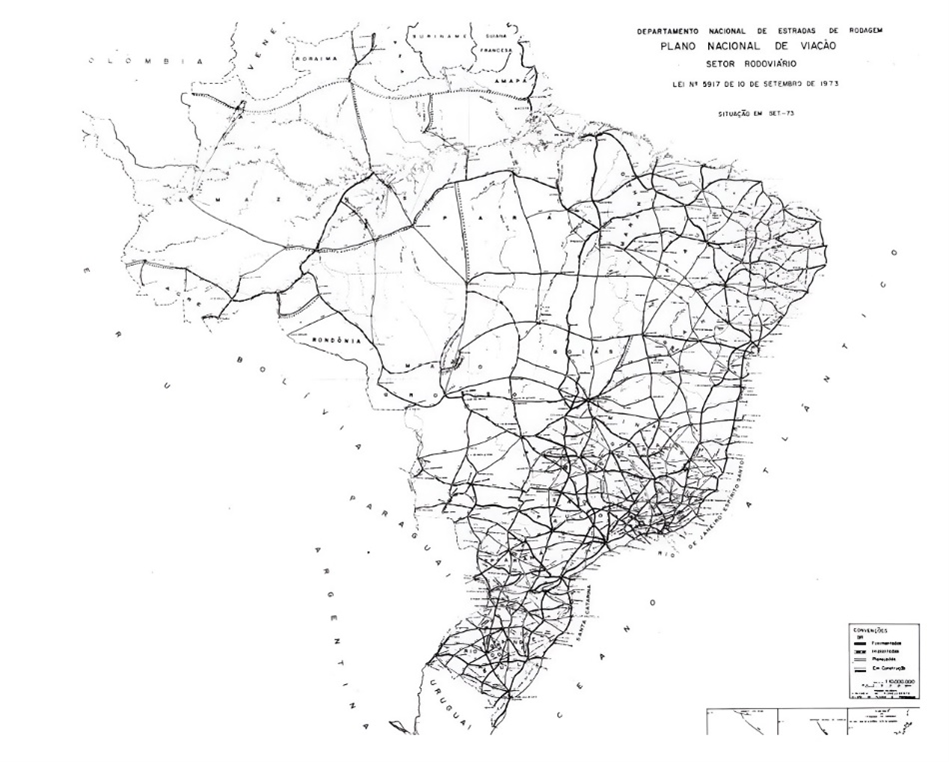
\includegraphics[width=0.75\linewidth]{figures/PNV1973.png}
\end{figure}
\clearpage

\begin{table}[p]\centering
\def\sym#1{\ifmmode^{#1}\else\(^{#1}\)\fi}
\begingroup
\renewcommand{\arraystretch}{1.3}
\caption{Income, Population, Urbanization, Agricultural Land Use and Access to World Market \label{tab:descriptives}}
\sbox{\tabbox}{%
\resizebox{\linewidth}{!}{
\begin{tabular}{l*{7}{c}}
\hline\hline
                    &\multicolumn{1}{c}{(1)}         &\multicolumn{1}{c}{(2)}         &\multicolumn{1}{c}{(3)}         &\multicolumn{1}{c}{(4)}         &\multicolumn{1}{c}{(5)}         &\multicolumn{1}{c}{(6)}         &\multicolumn{1}{c}{(7)}         \\
                    &         GDP         &  Population         &Urban Population         &Urban Population Share         &     Soybean         &      Coffee         &      Cattle         \\
\hline
Log Travel Time to Port&     -0.7947\sym{***}&     -0.4168\sym{***}&     -0.6810\sym{***}&     -0.2643\sym{***}&     -0.1554         &     -1.0941\sym{***}&      0.1738         \\
                    &    (0.1210)         &    (0.0691)         &    (0.0962)         &    (0.0557)         &    (0.3232)         &    (0.3459)         &    (0.2281)         \\
Observations        &         531         &         531         &         531         &         531         &         531         &         531         &         531         \\
$R^2$               &       0.250         &       0.164         &       0.226         &       0.164         &       0.001         &       0.060         &       0.011         \\
\hline\hline
\end{tabular}}
}
\usebox{\tabbox}
\begin{minipage}{\wd\tabbox}
    \vspace{0.1cm}
    {\footnotesize \sloppy \textit{Notes: } Each observation is a micro-region. Log travel time is the travel time to the closest international port on the 1970 road network. Economic outcomes are measured in 1970; the crop columns are harvested area from the 1974 Municipal Agricultural Production survey, and cattle is the herd converted at one head per hectare. Standard errors clustered at the state level are reported in parentheses. ***,**,* imply significance at the 1\%, 5\%, and 10\% levels, respectively.}
\end{minipage}
\endgroup
\end{table}

\clearpage

\begin{table}[p]\centering
\def\sym#1{\ifmmode^{#1}\else\(^{#1}\)\fi}
\begingroup
\renewcommand{\arraystretch}{1.3}
\caption{Long-Difference Regressions on Income and Population, 1970-2010 \label{tab:aggregate}}
\sbox{\tabbox}{%
\resizebox{\linewidth}{!}{
\begin{tabular}{l*{8}{c}}
\hline
\hline
&\multicolumn{2}{c}{GDP}                    &\multicolumn{2}{c}{Population}             &\multicolumn{2}{c}{Urban Population}       &\multicolumn{2}{c}{Urban Employment Share} \\\cmidrule(lr){2-3}\cmidrule(lr){4-5}\cmidrule(lr){6-7}\cmidrule(lr){8-9}
&\multicolumn{1}{c}{(1)}         &\multicolumn{1}{c}{(2)}         &\multicolumn{1}{c}{(3)}         &\multicolumn{1}{c}{(4)}         &\multicolumn{1}{c}{(5)}         &\multicolumn{1}{c}{(6)}         &\multicolumn{1}{c}{(7)}         &\multicolumn{1}{c}{(8)}         \\
&         OLS         &          IV         &         OLS         &          IV         &         OLS         &          IV         &         OLS         &          IV         \\
\hline
\multicolumn{8}{l}{\textbf{\textit{Panel A: Baseline controlling only for the initial value of the outcome}}} \\
$\Delta Log Travel Time$&       0.485\sym{*}  &       0.826\sym{**} &       0.056         &       0.454         &       0.366\sym{*}  &       0.969\sym{***}&       0.062         &       0.147\sym{***}\\
&     (0.269)         &     (0.355)         &     (0.193)         &     (0.277)         &     (0.207)         &     (0.212)         &     (0.057)         &     (0.056)         \\
Observations        &         531         &         531         &         531         &         531         &         531         &         531         &         531         &         531         \\
First-stage F stat  &                     &      82.721         &                     &      87.028         &                     &      81.812         &                     &      66.947         \\
\hline
\multicolumn{8}{l}{\linebreak \textbf{\textit{Panel B: Panel (A) including state fixed effects}}} \\
$\Delta Log Travel Time$&       0.149         &       0.340         &      -0.197         &       0.043         &       0.038         &       0.428\sym{***}&      -0.058         &       0.079\sym{**} \\
&     (0.212)         &     (0.310)         &     (0.144)         &     (0.244)         &     (0.113)         &     (0.148)         &     (0.040)         &     (0.034)         \\
Observations        &         528         &         528         &         528         &         528         &         528         &         528         &         528         &         528         \\
First-stage F stat  &                     &      66.786         &                     &      64.828         &                     &      64.029         &                     &      60.368         \\
\hline
\multicolumn{8}{l}{\linebreak \textbf{\textit{Panel C: Panel (B) including covariates for additional geographical traits}}} \\
$\Delta Log Travel Time$&       0.057         &       0.272         &      -0.222         &       0.076         &      -0.075         &       0.329\sym{**} &      -0.079\sym{**} &       0.048         \\
&     (0.231)         &     (0.287)         &     (0.167)         &     (0.230)         &     (0.152)         &     (0.148)         &     (0.038)         &     (0.040)         \\
Observations        &         528         &         528         &         528         &         528         &         528         &         528         &         528         &         528         \\
First-stage F stat  &                     &      59.867         &                     &      58.992         &                     &      57.661         &                     &      55.388         \\
\hline\hline
\end{tabular}}
}
\usebox{\tabbox}
\begin{minipage}{\wd\tabbox}
    \vspace{0.1cm}
    {\footnotesize \sloppy \textit{Notes: } Each observation is a micro-region. Log change in travel time on roads is instrumented by the change in travel times on the predicted road network. The predicted road network is created by geo-referencing the PNV National Transportation Plan in 1973. The Kleibergen-Paap F-statistic (First-stage F stat) for weak identification is reported for IV estimates. Standard errors clustered at the state level are reported in parentheses. ***,**,* imply significance at the 1\%, 5\%, and 10\% levels, respectively.}
\end{minipage}
\endgroup
\end{table}

\clearpage

\begin{table}[p]\centering
\def\sym#1{\ifmmode^{#1}\else\(^{#1}\)\fi}
\begingroup
\renewcommand{\arraystretch}{1.3}
\caption{Long-Difference Regressions on Agricultural Land Use, 1974-2010 \label{tab:landuse}}
\sbox{\tabbox}{%
\resizebox{\linewidth}{!}{
\begin{tabular}{l*{8}{c}}
\hline \hline
&\multicolumn{2}{c}{Total Cropland}         &\multicolumn{2}{c}{Sensitive}              &\multicolumn{2}{c}{Insensitive}            &\multicolumn{2}{c}{Pasture}                \\\cmidrule(lr){2-3}\cmidrule(lr){4-5}\cmidrule(lr){6-7}\cmidrule(lr){8-9}
&\multicolumn{1}{c}{(1)}         &\multicolumn{1}{c}{(2)}         &\multicolumn{1}{c}{(3)}         &\multicolumn{1}{c}{(4)}         &\multicolumn{1}{c}{(5)}         &\multicolumn{1}{c}{(6)}         &\multicolumn{1}{c}{(7)}         &\multicolumn{1}{c}{(8)}         \\
&         OLS         &          IV         &         OLS         &          IV         &         OLS         &          IV         &         OLS         &          IV         \\
\hline
\multicolumn{8}{l}{\textbf{\textit{Panel A: Baseline controlling only for the initial value of the outcome}}} \\
$\Delta Log Travel Time$&       1.296\sym{**} &       2.279\sym{***}&       5.263\sym{***}&       7.173\sym{***}&      -0.392         &       1.192         &       1.191\sym{***}&       2.456\sym{***}\\
&     (0.509)         &     (0.571)         &     (1.836)         &     (2.097)         &     (0.762)         &     (1.061)         &     (0.327)         &     (0.663)         \\
Observations        &         531         &         531         &         531         &         531         &         531         &         531         &         531         &         531         \\
First-stage F stat  &                     &      84.111         &                     &      79.437         &                     &      79.649         &                     &      88.191         \\
\hline
\multicolumn{8}{l}{\linebreak \textbf{\textit{Panel B: Panel (A) including state fixed effects}}} \\
$\Delta Log Travel Time$&       0.139         &       0.623         &       3.173\sym{**} &       4.815\sym{**} &       0.391         &       1.606         &       0.265         &       0.958         \\
&     (0.447)         &     (0.534)         &     (1.284)         &     (1.769)         &     (0.628)         &     (1.172)         &     (0.421)         &     (0.655)         \\
Observations        &         528         &         528         &         528         &         528         &         528         &         528         &         528         &         528         \\
First-stage F stat  &                     &      63.728         &                     &      63.092         &                     &      61.490         &                     &      64.284         \\
\hline
\multicolumn{8}{l}{\linebreak \textbf{\textit{Panel C: Panel (B) including covariates for additional geographical traits}}} \\
$\Delta Log Travel Time$&      -0.261         &      -0.035         &       2.368\sym{*}  &       3.732\sym{*}  &      -0.062         &       1.050         &      -0.066         &       0.465         \\
&     (0.442)         &     (0.591)         &     (1.255)         &     (1.928)         &     (0.644)         &     (1.239)         &     (0.359)         &     (0.495)         \\
Observations        &         528         &         528         &         528         &         528         &         528         &         528         &         528         &         528         \\
First-stage F stat  &                     &      56.909         &                     &      58.199         &                     &      55.953         &                     &      52.091         \\
\hline\hline
\end{tabular}}
}
\usebox{\tabbox}
\begin{minipage}{\wd\tabbox}
    \vspace{0.1cm}
    {\footnotesize \sloppy \textit{Notes: } Each observation is a micro-region. Log change in travel time on roads is instrumented by the change in travel times on the predicted road network. The predicted road network is created by geo-referencing the PNV National Transportation Plan in 1973. The Kleibergen-Paap F-statistic (First-stage F stat) for weak identification is reported for IV estimates. Standard errors clustered at the state level are reported in parentheses. Outcomes are the log change in category land area, with micro-regions recording no area assigned a minimum value of one. Total cropland excludes pasture, which is the cattle herd converted at one head per hectare. ***,**,* imply significance at the 1\%, 5\%, and 10\% levels, respectively.}
\end{minipage}
\endgroup
\end{table}

\clearpage

\begin{table}[p]\centering
\def\sym#1{\ifmmode^{#1}\else\(^{#1}\)\fi}
\begingroup
\renewcommand{\arraystretch}{1.3}
\caption{Extensive Margin of Agricultural Land Use, 1974-2010 \label{tab:extensive}}
\sbox{\tabbox}{%
\begin{tabular}{l*{4}{c}}
\hline\hline
                    &\multicolumn{2}{c}{Sensitive}              &\multicolumn{2}{c}{Insensitive}            \\\cmidrule(lr){2-3}\cmidrule(lr){4-5}
                    &\multicolumn{1}{c}{(1)}         &\multicolumn{1}{c}{(2)}         &\multicolumn{1}{c}{(3)}         &\multicolumn{1}{c}{(4)}         \\
                    &         LPM         &      Probit         &         LPM         &      Probit         \\
\hline
$\Delta Log Travel Time$&       0.216\sym{**} &       0.230\sym{*}  &       0.076         &       0.134         \\
                    &     (0.101)         &     (0.131)         &     (0.065)         &     (0.138)         \\
Observations        &         528         &         394         &         528         &         383         \\
First-stage F stat  &      58.304         &                     &      58.304         &                     \\
\hline\hline
\end{tabular}
}
\usebox{\tabbox}
\begin{minipage}{\wd\tabbox}
    \vspace{0.1cm}
    {\footnotesize \sloppy \textit{Notes: } Each observation is a micro-region. Log change in travel time on roads is instrumented by the change in travel times on the predicted road network. The predicted road network is created by geo-referencing the PNV National Transportation Plan in 1973. Dependent variables are defined as a dummy equal to 1 if the micro-region recorded no area in the category in 1974 but positive area in 2010. The reported coefficients for Probit Regressions are the directly interpretable marginal effect. ***,**,* imply significance at the 1\%, 5\%, and 10\% levels, respectively.}
\end{minipage}
\endgroup
\end{table}

\clearpage

\begin{figure}[p!]
    \centering
    \caption{Time-varying effects on Income and Population}
    \label{fig:es_agg}

    \begin{subfigure}{0.48\textwidth}
        \centering
        \caption{GDP}
        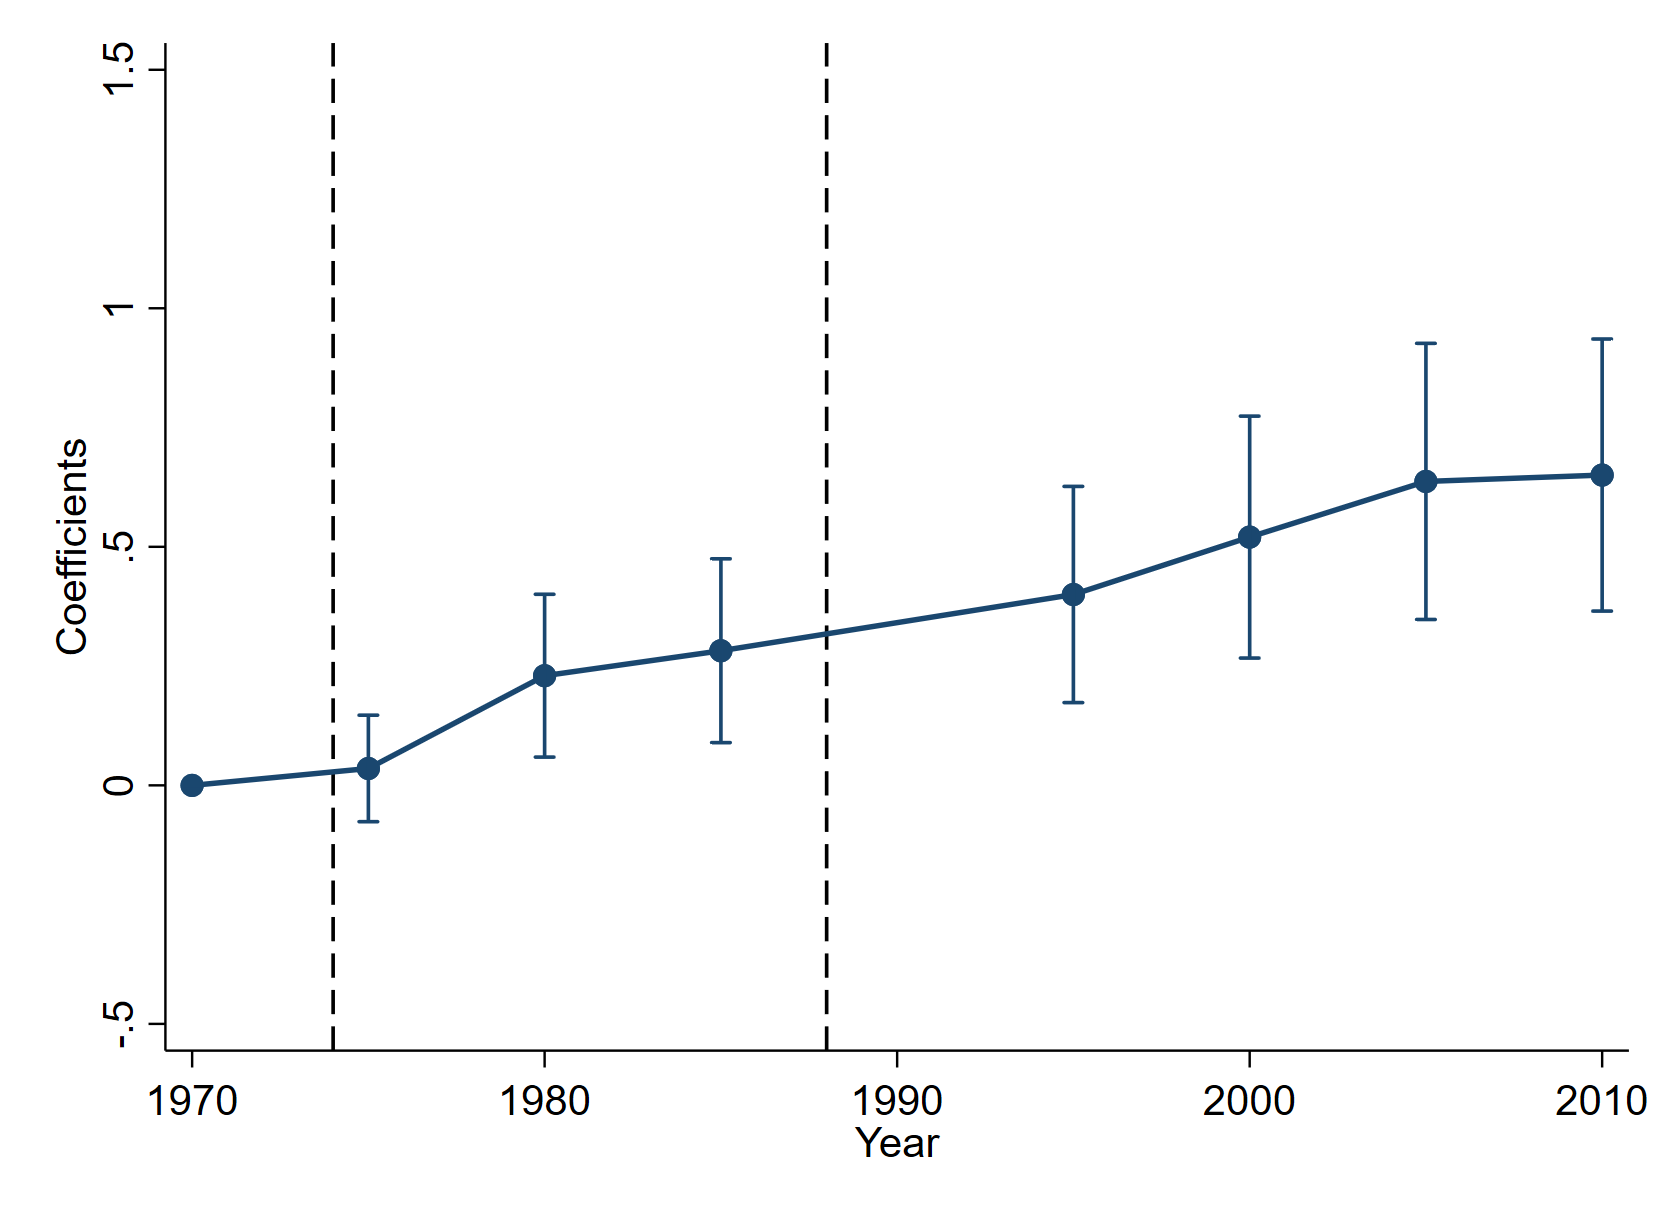
\includegraphics[width=\textwidth]{figures/gdp.png}
        \label{gdp}
    \end{subfigure}
    \hfill 
    \begin{subfigure}{0.48\textwidth}
        \centering
        \caption{Population}
        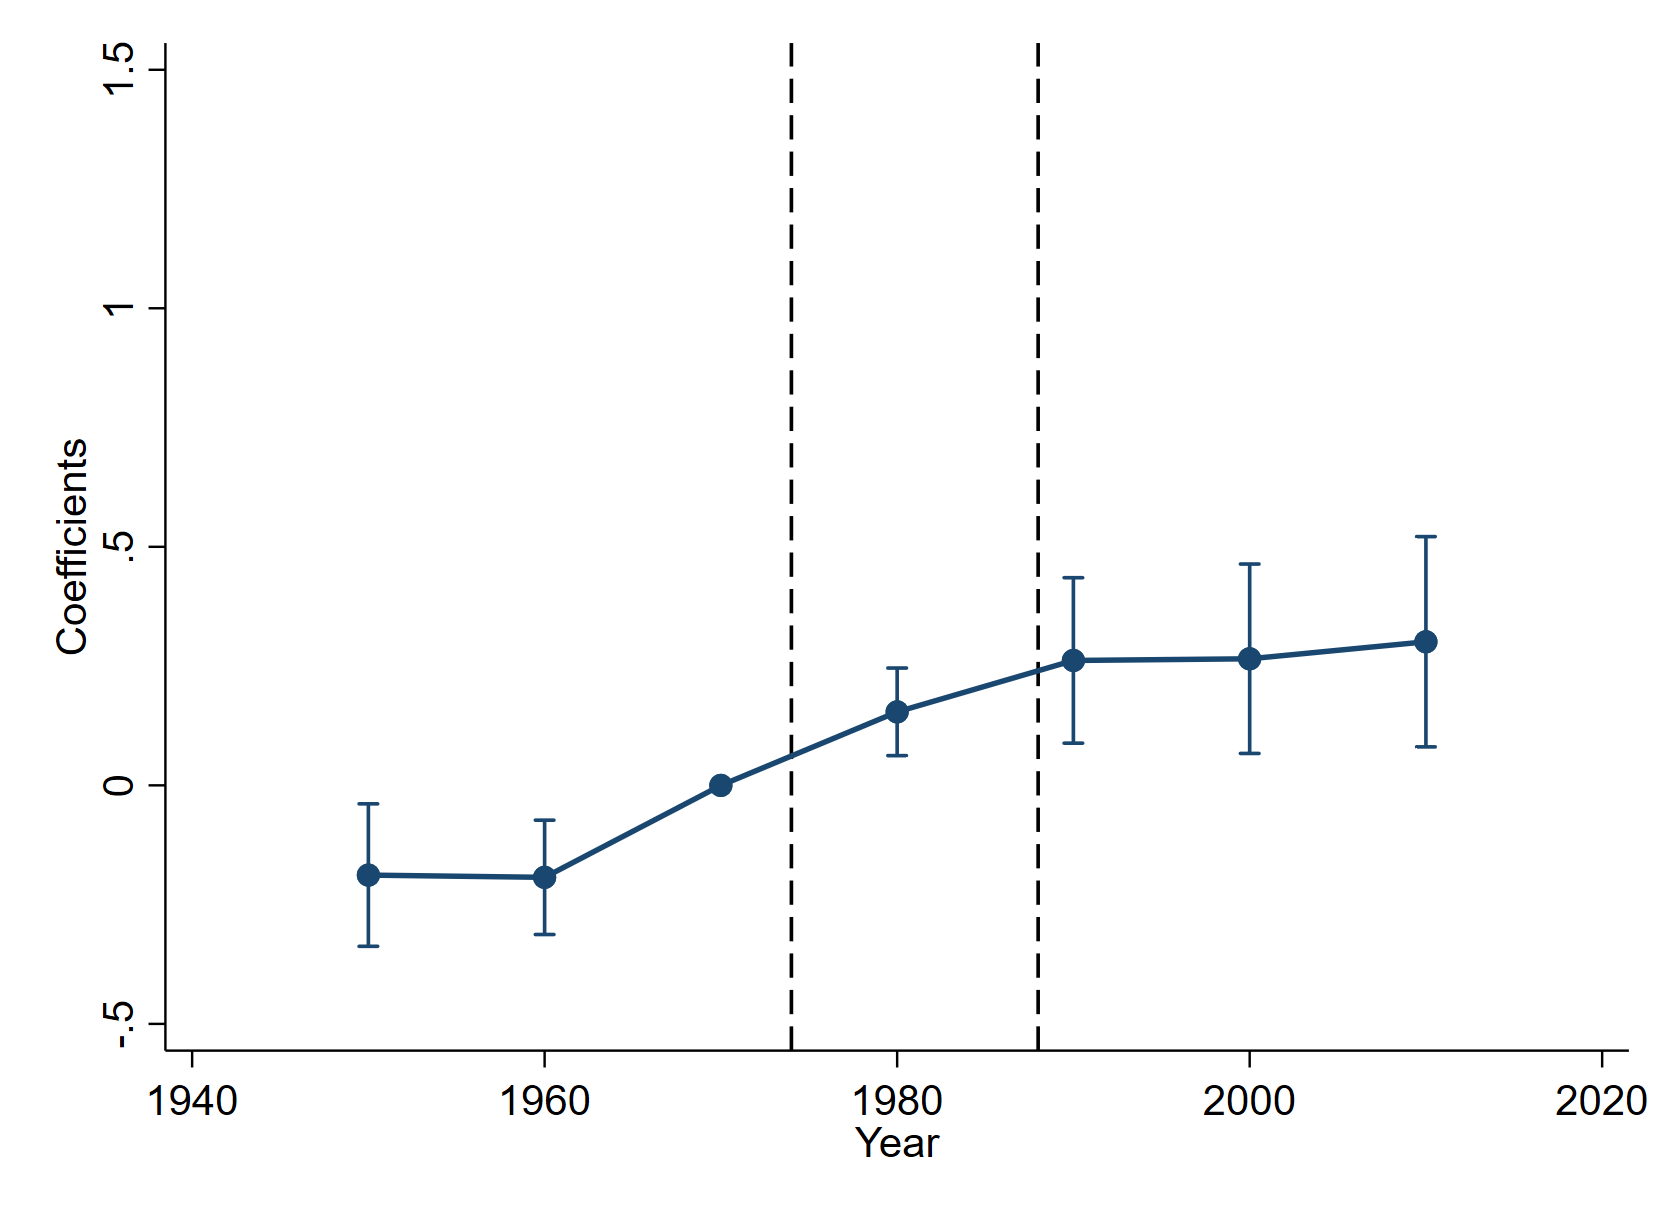
\includegraphics[width=\textwidth]{figures/pop.png}
        \label{pop}
    \end{subfigure}
    
    \vspace{10pt}

    \begin{subfigure}{0.48\textwidth}
        \centering
        \caption{Urban Population}
        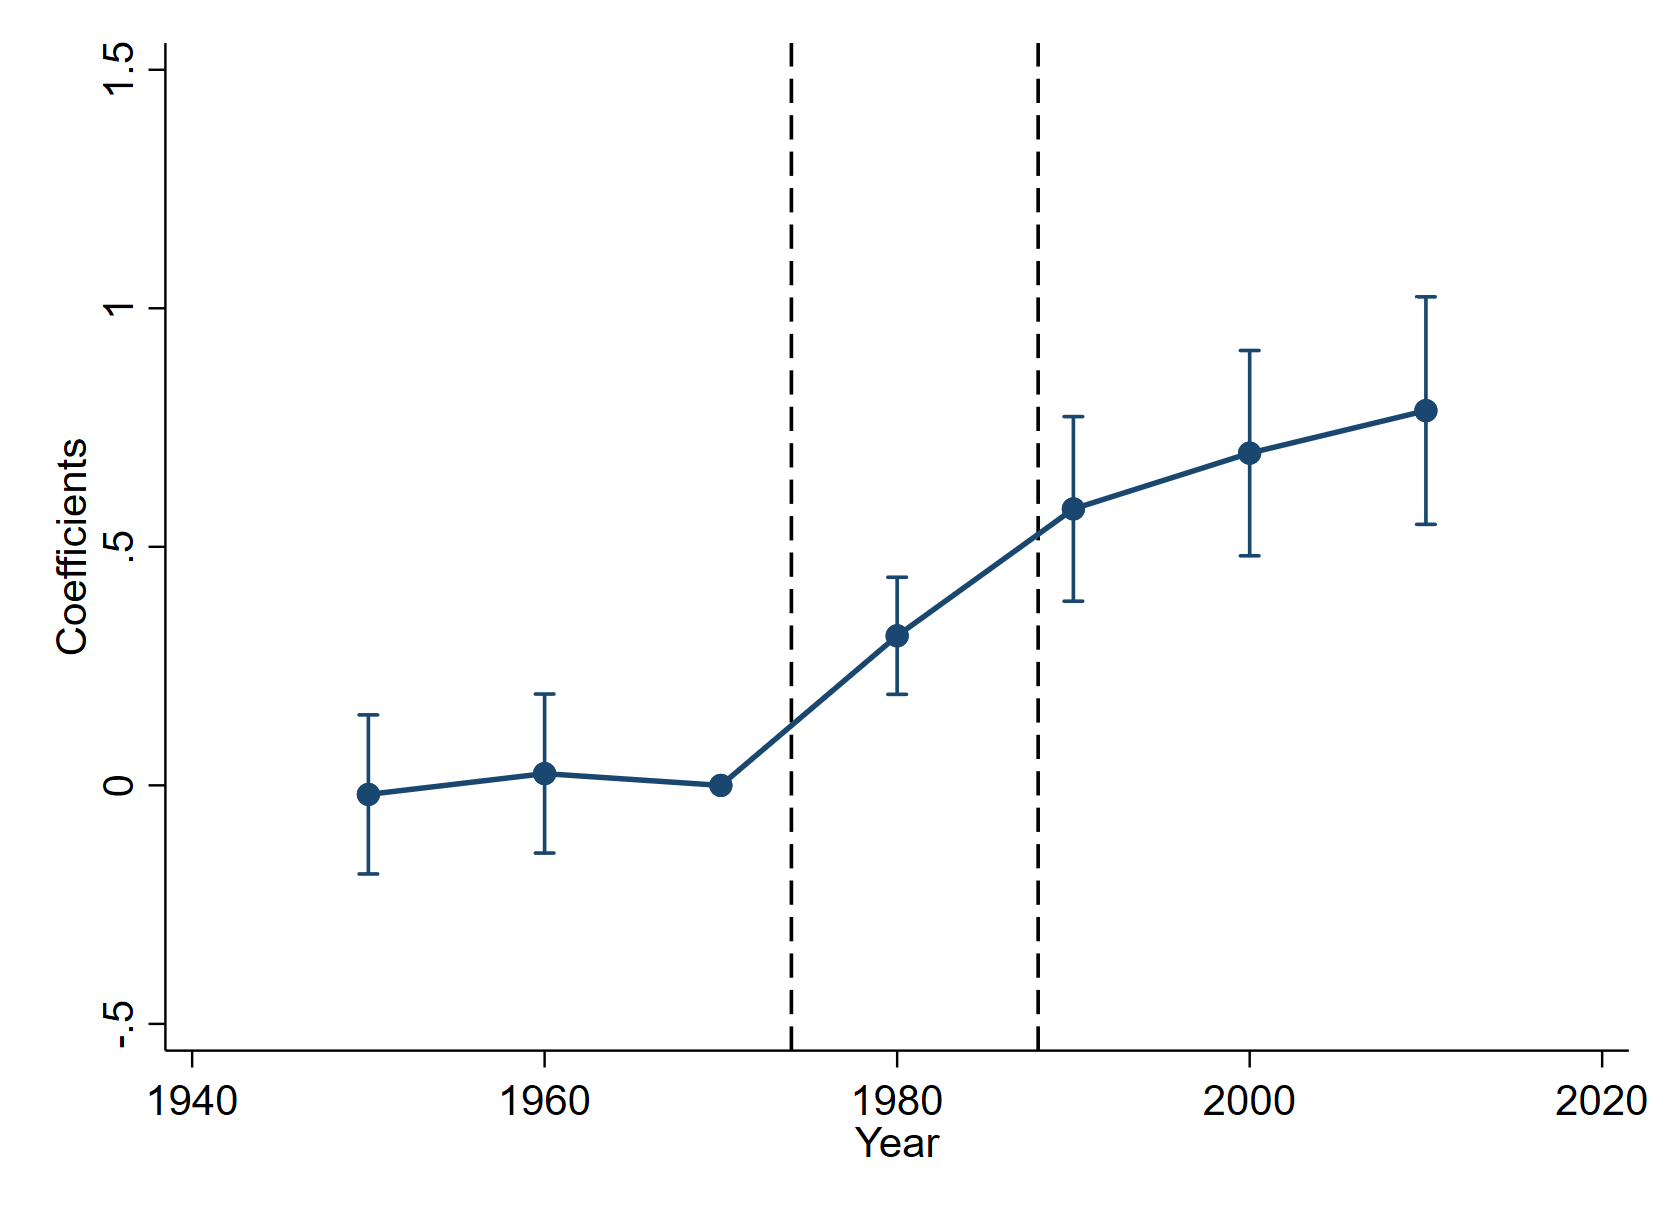
\includegraphics[width=\textwidth]{figures/urbpop.png}
        \label{urbpop}
    \end{subfigure}
    \hfill
    \begin{subfigure}{0.48\textwidth}
        \centering
        \caption{Urban Population Share}
        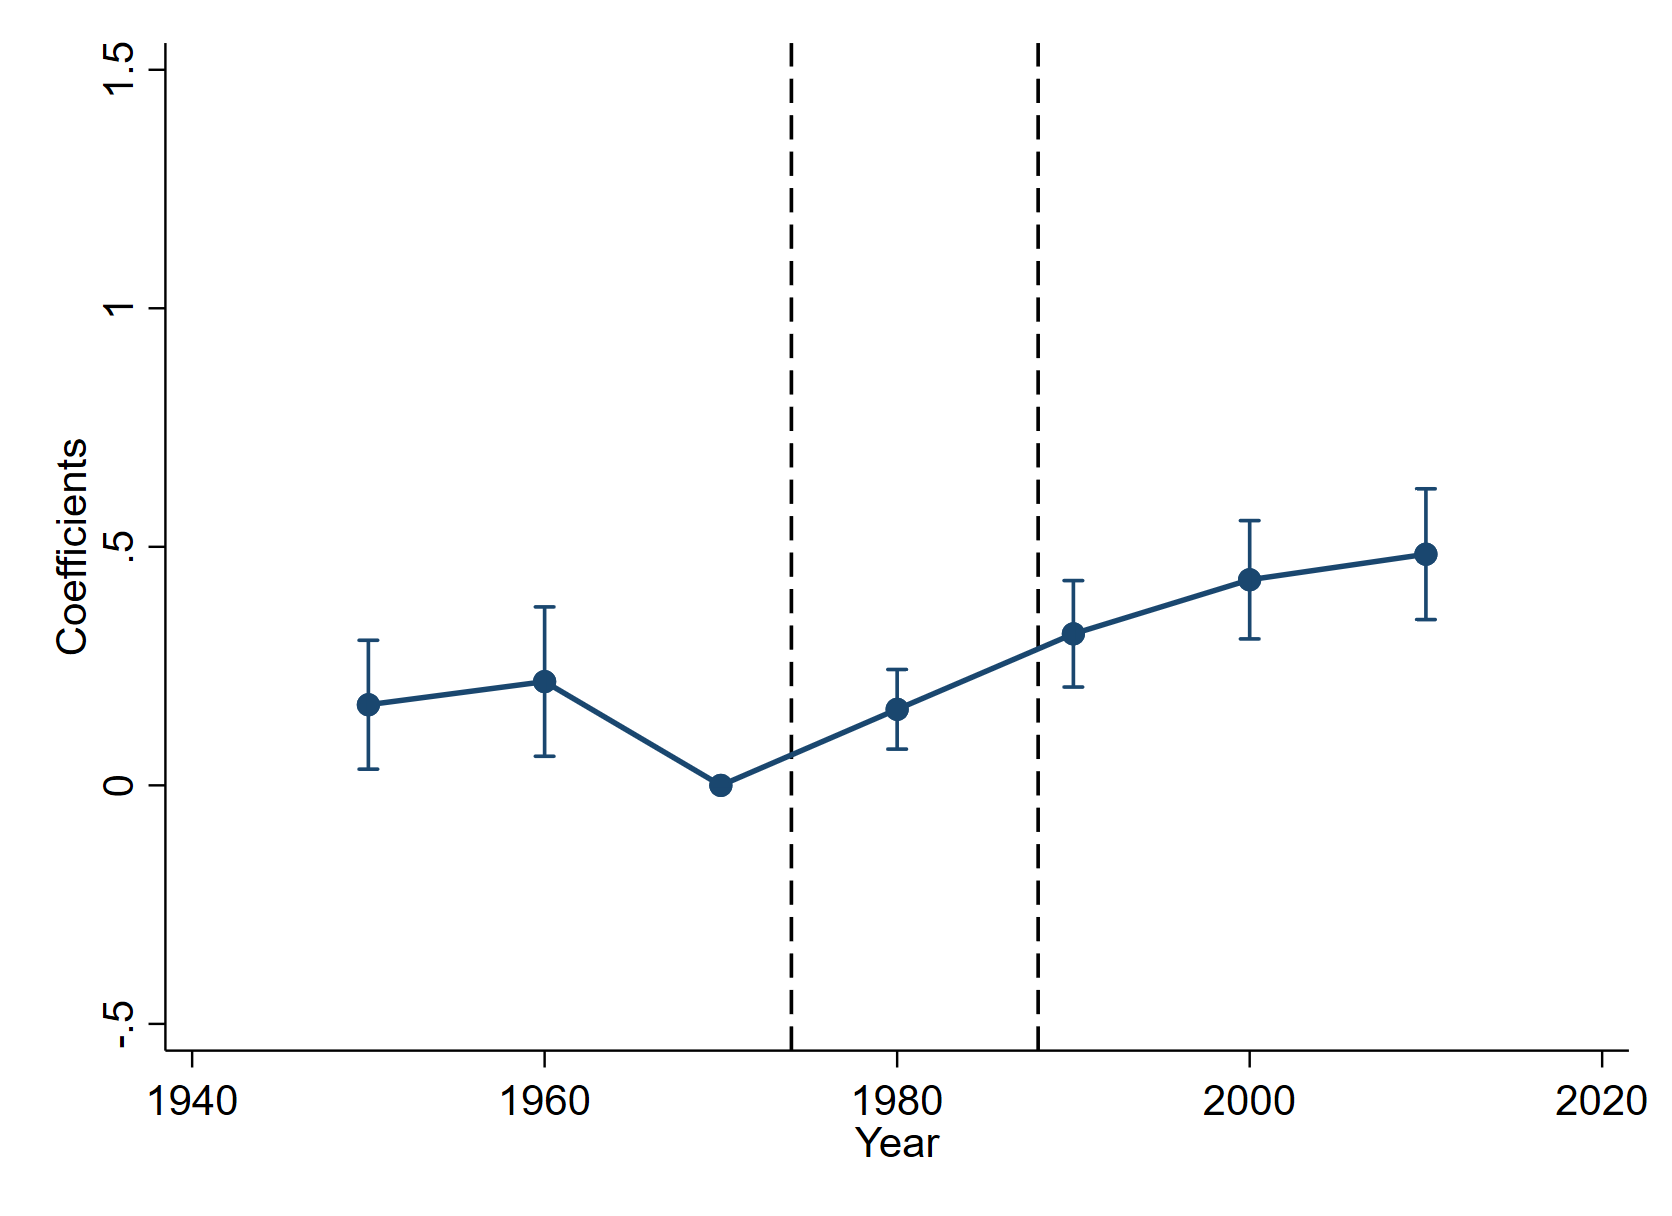
\includegraphics[width=\textwidth]{figures/urbshare.png}
        \label{urbshare}
    \end{subfigure}

    
\end{figure}
\clearpage

\begin{figure}[p!]
    \centering
    \caption{Time-varying effects on Agricultural Land Use}
    \label{fig:es_ag}
    
    \begin{subfigure}{0.48\textwidth}
        \centering
        \caption{Transport-Cost-Sensitive}
        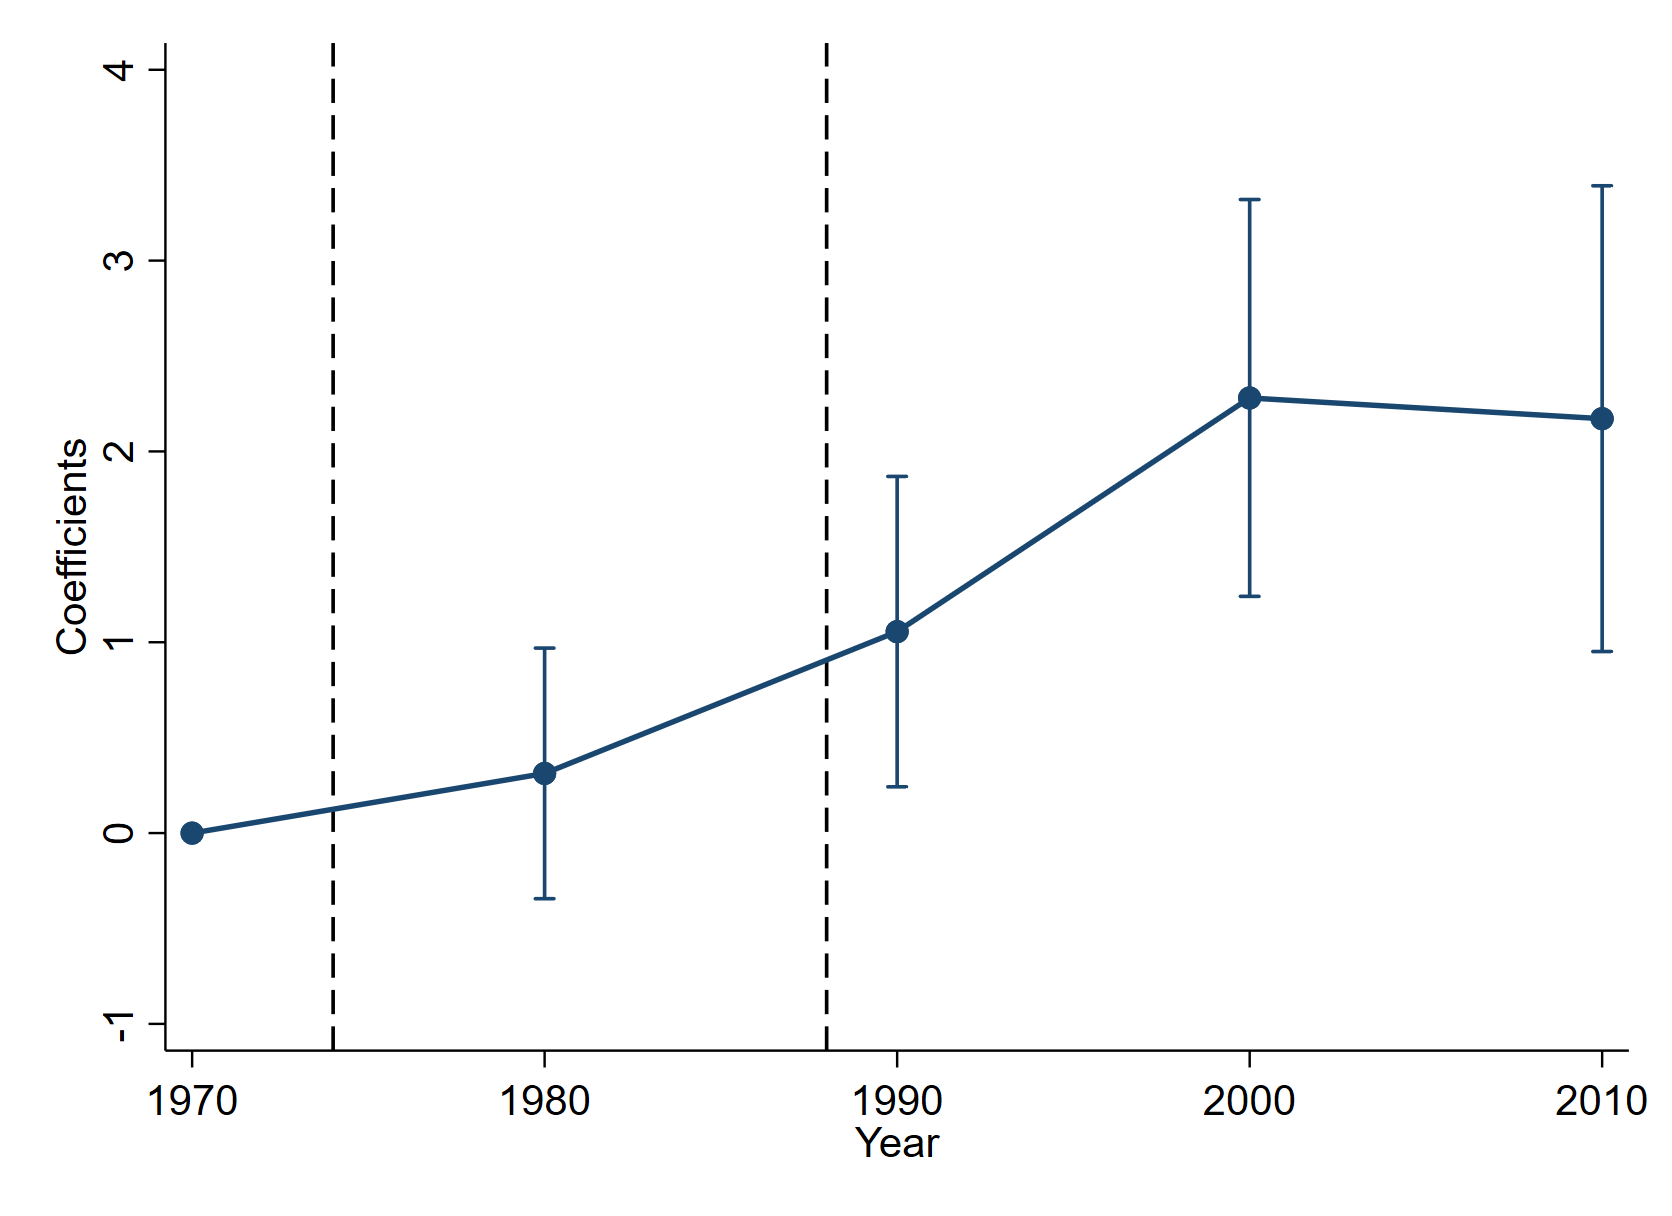
\includegraphics[width=\textwidth]{figures/sensitive.png}
        \label{sensitive}
    \end{subfigure}
    \begin{subfigure}{0.48\textwidth}
        \centering
        \caption{Transport-Cost-Insensitive}
        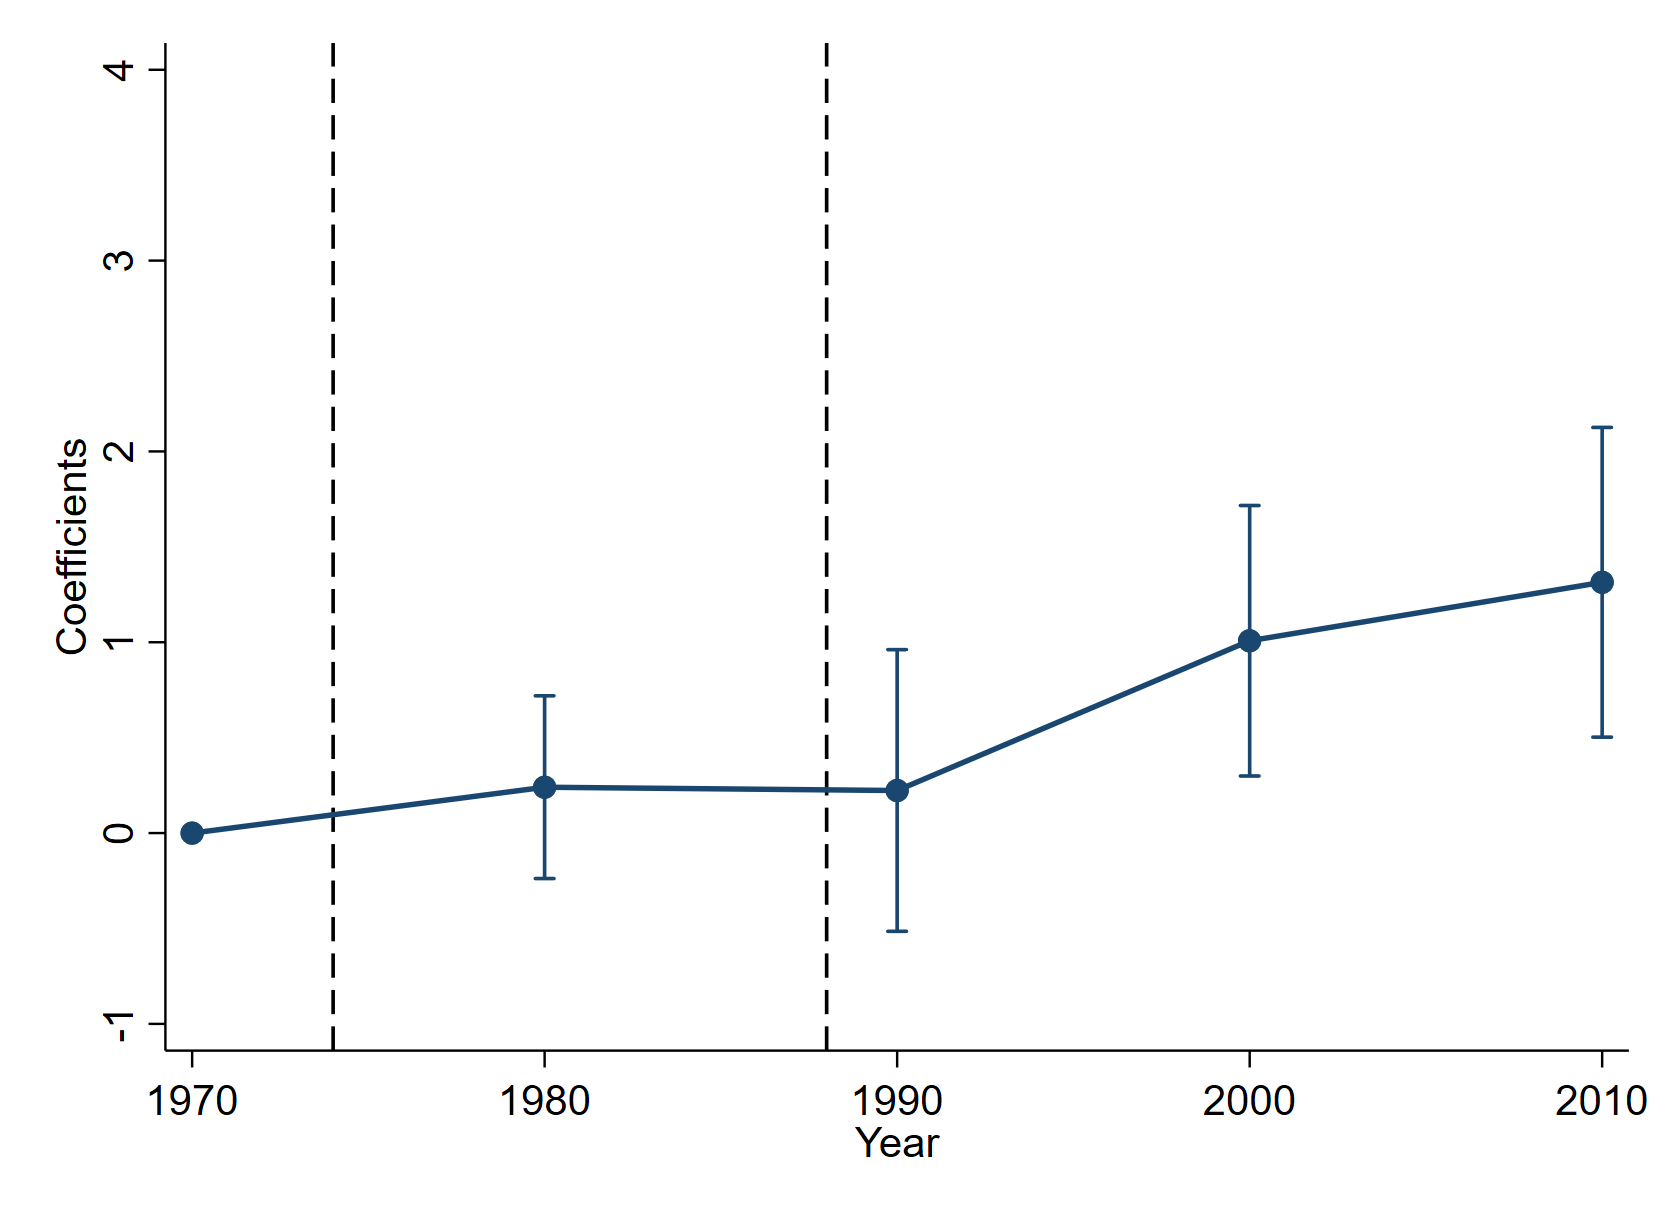
\includegraphics[width=\textwidth]{figures/insensitive.png}
        \label{insensitive}
    \end{subfigure}
    \begin{subfigure}{0.48\textwidth}
        \centering
        \caption{Pasture}
        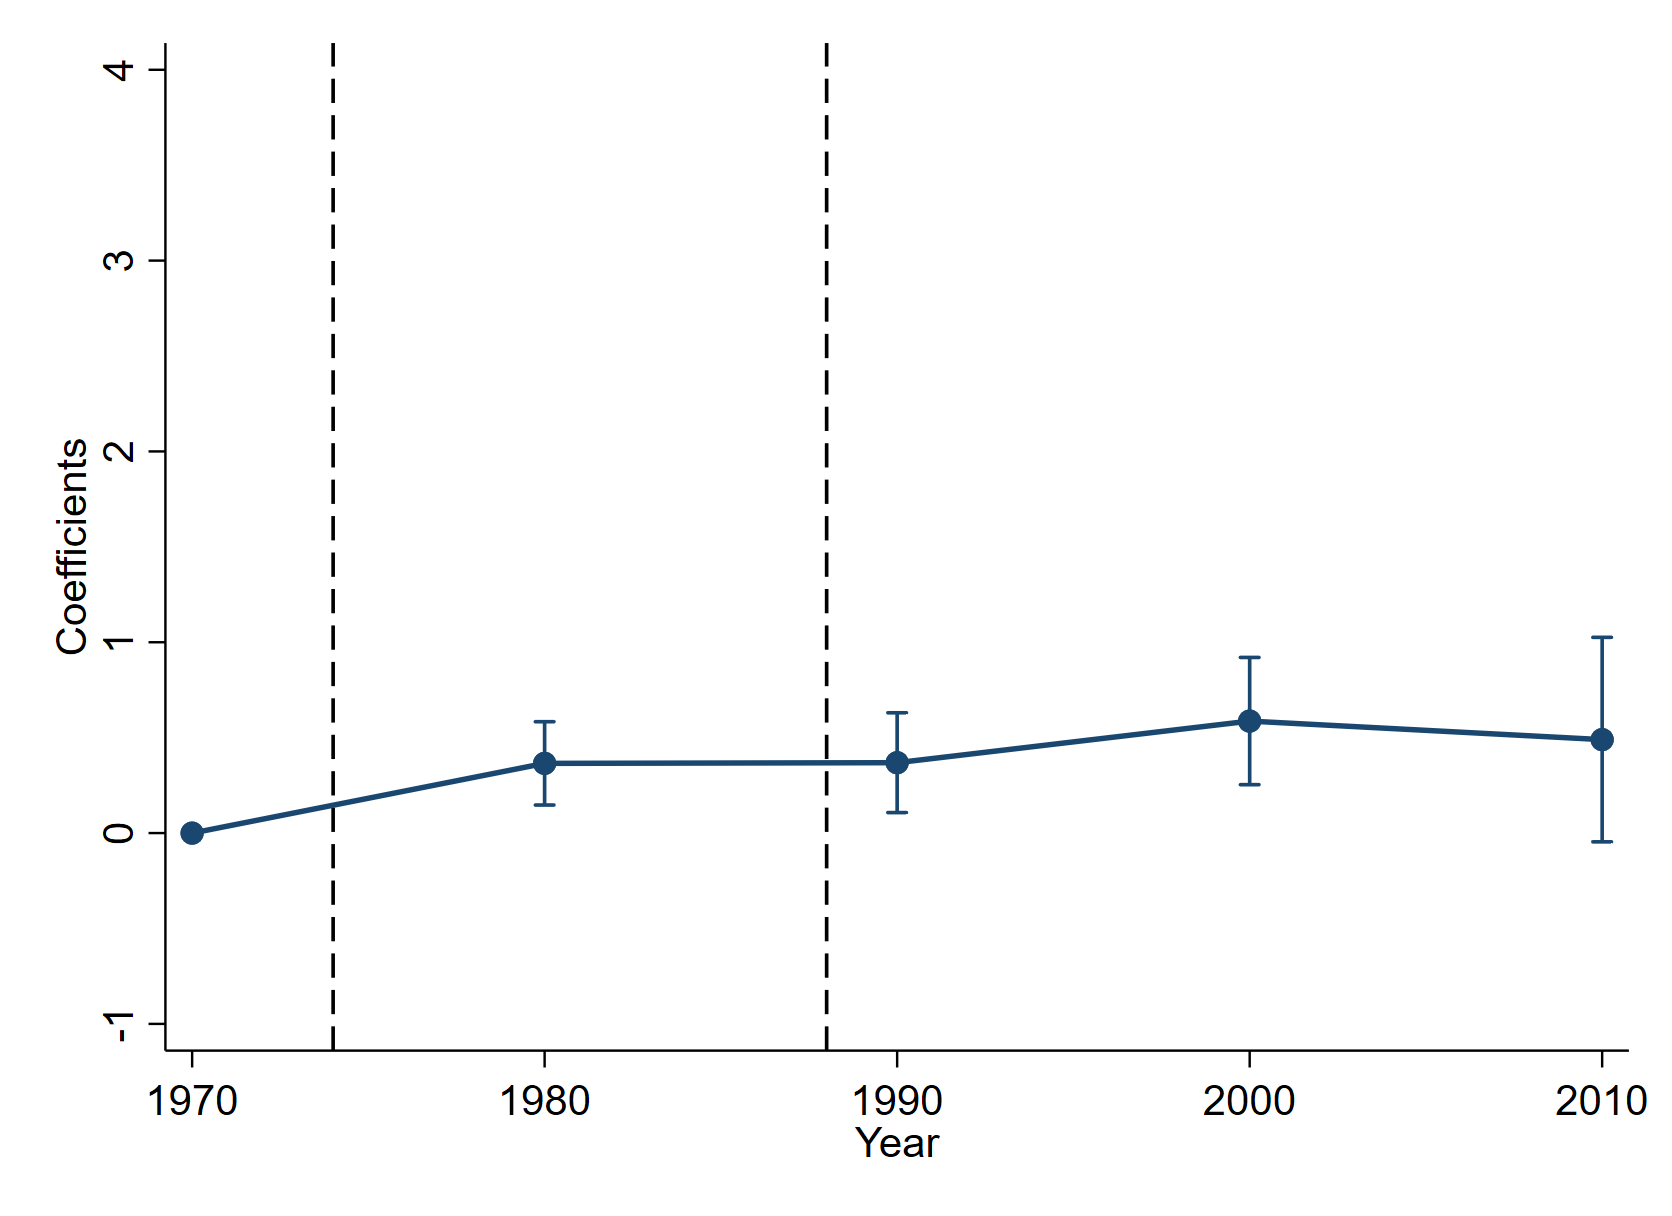
\includegraphics[width=\textwidth]{figures/pasture.png}
        \label{pasture}
    \end{subfigure}
\end{figure}
\clearpage

\begin{table}[p]\centering
\def\sym#1{\ifmmode^{#1}\else\(^{#1}\)\fi}
\begingroup
\renewcommand{\arraystretch}{1.3}
\caption{Pooled Transport-Sensitivity Interaction, Traded Crops, 1974-2010 \label{tab:pooledtau}}
\sbox{\tabbox}{%
\begin{tabular}{l*{4}{c}}
\hline\hline
                    &\multicolumn{2}{c}{$\Delta$ Log Area}      &\multicolumn{2}{c}{$\Delta$ Land Share}    \\\cmidrule(lr){2-3}\cmidrule(lr){4-5}
                    &\multicolumn{1}{c}{(1)}         &\multicolumn{1}{c}{(2)}         &\multicolumn{1}{c}{(3)}         &\multicolumn{1}{c}{(4)}         \\
                    &Binary $\tau$         &Log Value/Ton         &Binary $\tau$         &Log Value/Ton         \\
\hline
$\tau_g \times \Delta Log Travel Time$&      2.0910\sym{***}&     -1.4756\sym{***}&      0.0300\sym{***}&     -0.0217\sym{***}\\
                    &    (0.4409)         &    (0.2838)         &    (0.0093)         &    (0.0063)         \\
\hline
Product FE          &         Yes         &         Yes         &         Yes         &         Yes         \\
Micro-region FE     &         Yes         &         Yes         &         Yes         &         Yes         \\
Observations        &        4248         &        4248         &        4248         &        4248         \\
First-stage F stat  &     167.872         &     167.872         &     167.872         &     167.872         \\
\hline\hline
\end{tabular}
}
\usebox{\tabbox}
\begin{minipage}{\wd\tabbox}
    \vspace{0.1cm}
    {\footnotesize \sloppy \textit{Notes: } Each observation is a traded crop in a micro-region, over the long difference 1974-2010. The interaction of transport-cost sensitivity with the change in log travel time is instrumented by its interaction with the PIN-induced reduction. Binary $\tau$ contrasts the transport-cost-sensitive and insensitive categories; log value per tonne is the national unit value in 2010. Standard errors clustered at the micro-region level are reported in parentheses. ***,**,* imply significance at the 1\%, 5\%, and 10\% levels, respectively.}
\end{minipage}
\endgroup
\end{table}

\clearpage

\begin{table}[p]\centering
\def\sym#1{\ifmmode^{#1}\else\(^{#1}\)\fi}
\begingroup
\renewcommand{\arraystretch}{1.3}
\caption{Interaction with Micro-Region Traits \label{tab:heterogeneity}}
\sbox{\tabbox}{%
\resizebox{\linewidth}{!}{
\begin{tabular}{l*{4}{c}}
\hline \hline
&\multicolumn{1}{c}{(1)}         &\multicolumn{1}{c}{(2)}         &\multicolumn{1}{c}{(3)}         &\multicolumn{1}{c}{(4)}         \\
&         GDP         &  Population         &Urban Population         &Urban Employment Share         \\
\hline
\multicolumn{4}{l}{\textbf{\textit{Panel A: Distance to Waterway}}} \\
$\Delta Log Travel Time$&       0.312         &       0.237         &       0.638         &       0.107         \\
&     (0.678)         &     (0.517)         &     (0.499)         &     (0.113)         \\
$\Delta Log Travel Time \times Distance To Waterway$&      -0.058         &      -0.194         &      -0.406         &      -0.079         \\
&     (0.702)         &     (0.424)         &     (0.504)         &     (0.127)         \\
Observations        &         528         &         528         &         528         &         528         \\
State FE            &         Yes         &         Yes         &         Yes         &         Yes         \\
Initial level of outcome&         Yes         &         Yes         &         Yes         &         Yes         \\
Geographical Characteristics&         Yes         &         Yes         &         Yes         &         Yes         \\
\hline
\multicolumn{4}{l}{\linebreak \textbf{\textit{Panel B: Center-West Region}}} \\
$\Delta Log Travel Time$&       0.228         &       0.014         &       0.257         &       0.038         \\
&     (0.305)         &     (0.245)         &     (0.174)         &     (0.044)         \\
$\Delta Log Travel Time \times CenterWest$&       1.051         &       1.571         &       1.783         &       0.239         \\
&     (1.369)         &     (1.275)         &     (1.748)         &     (0.208)         \\
Observations        &         528         &         528         &         528         &         528         \\
State FE            &         Yes         &         Yes         &         Yes         &         Yes         \\
Initial level of outcome&         Yes         &         Yes         &         Yes         &         Yes         \\
Geographical Characteristics&         Yes         &         Yes         &         Yes         &         Yes         \\
\hline
\multicolumn{4}{l}{\linebreak \textbf{\textit{Panel C: Distance to State Capital}}} \\
$\Delta Log Travel Time$&       0.866\sym{**} &       0.516\sym{*}  &       0.927\sym{***}&       0.023         \\
&     (0.317)         &     (0.286)         &     (0.265)         &     (0.071)         \\
$\Delta Log Travel Time \times Distance To Capital$&      -1.239\sym{***}&      -0.736\sym{**} &      -1.121\sym{**} &      -0.006         \\
&     (0.375)         &     (0.286)         &     (0.428)         &     (0.130)         \\
Observations        &         528         &         528         &         528         &         528         \\
State FE            &         Yes         &         Yes         &         Yes         &         Yes         \\
Initial level of outcome&         Yes         &         Yes         &         Yes         &         Yes         \\
Geographical Characteristics&         Yes         &         Yes         &         Yes         &         Yes         \\
\hline\hline
\end{tabular}}
}
\usebox{\tabbox}
\begin{minipage}{\wd\tabbox}
    \vspace{0.1cm}
    {\footnotesize \sloppy \textit{Notes: } Each observation is a micro-region. Log change in travel time on roads is instrumented by the change in travel times on the predicted road network. The predicted road network is created by geo-referencing the PNV National Transportation Plan in 1973. The Kleibergen-Paap F-statistic (First-stage F stat) for weak identification is reported for IV estimates. Standard errors clustered at the state level are reported in parentheses. ***,**,* imply significance at the 1\%, 5\%, and 10\% levels, respectively.}
\end{minipage}
\endgroup
\end{table}

\clearpage

\begin{figure}[p!]
    \centering
    \caption{Time-varying effects on Travel Time}
    \label{fig:es_tt}
    
    \begin{subfigure}{0.48\textwidth}
        \centering
        \caption{TWFE}
        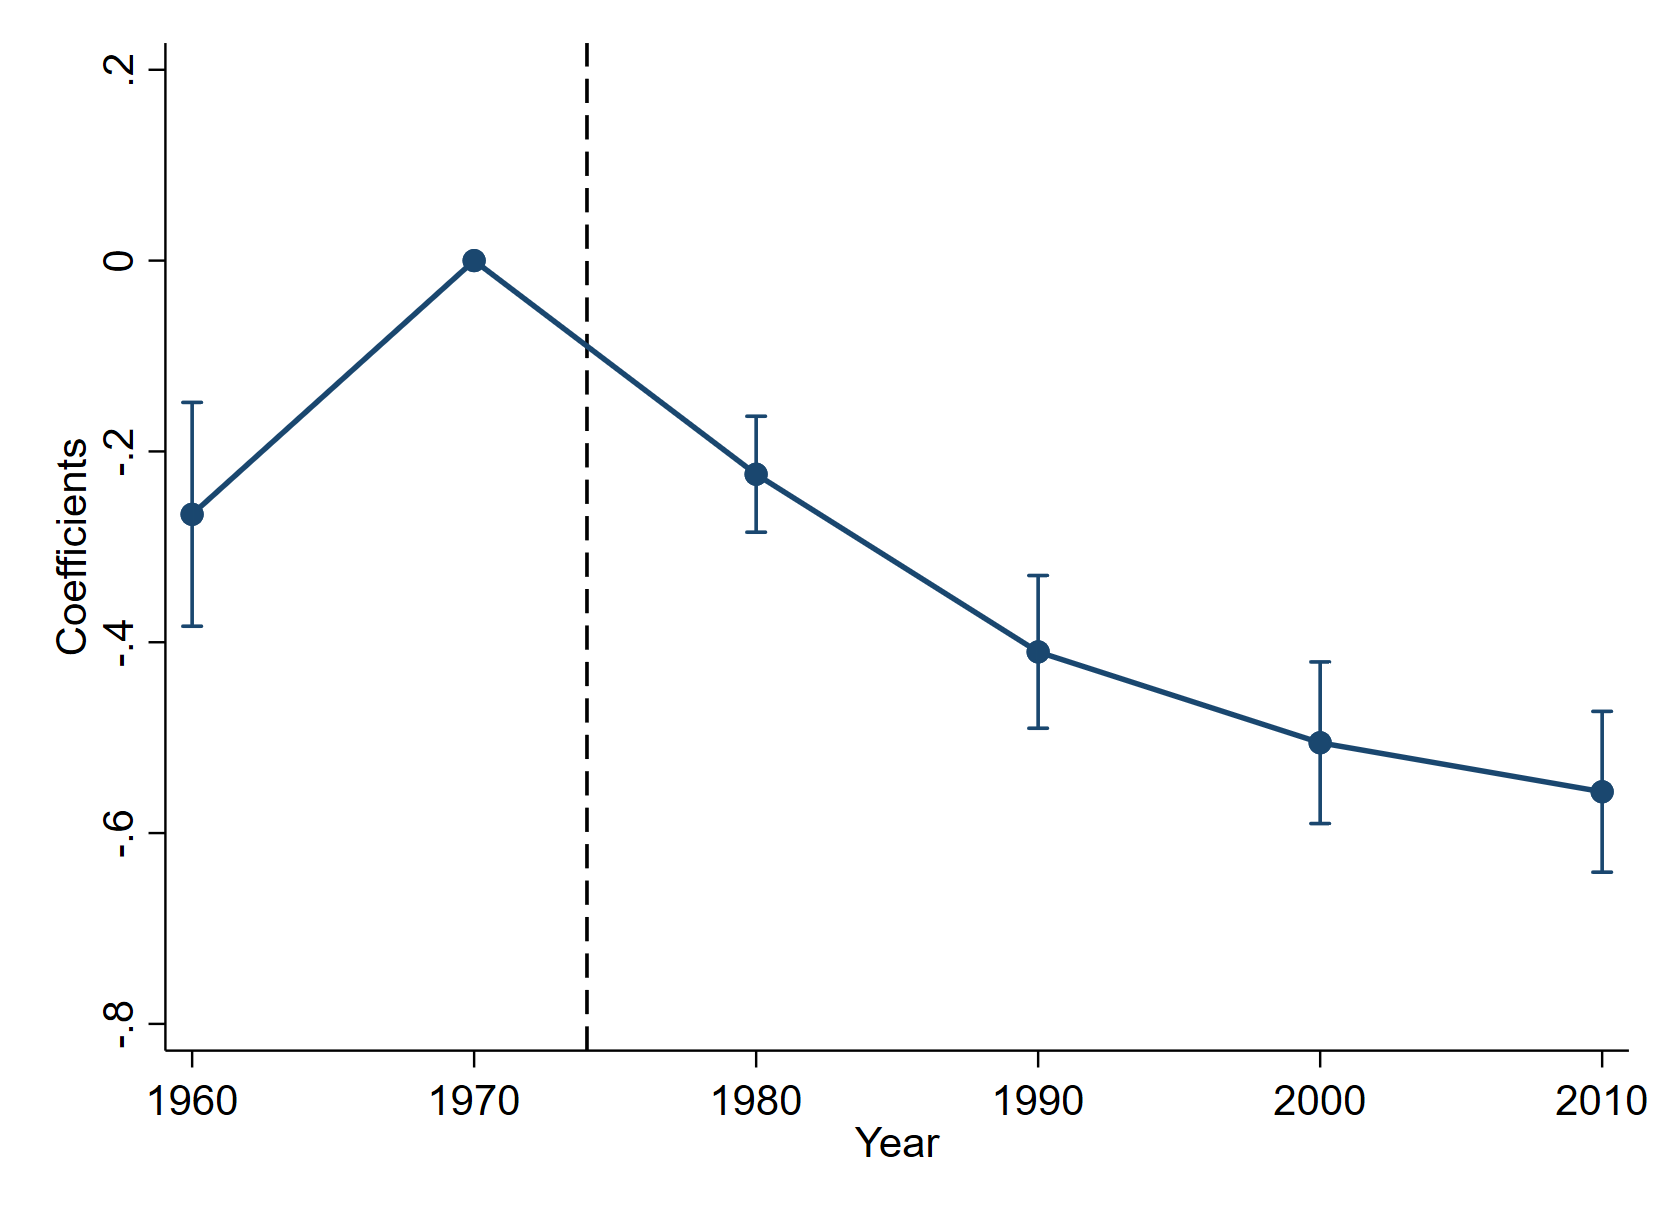
\includegraphics[width=\textwidth]{figures/road_twfe.png}
        \label{road}
    \end{subfigure}
    \begin{subfigure}{0.48\textwidth}
        \centering
        \caption{Borusyak et al. (2022) Estimator}
        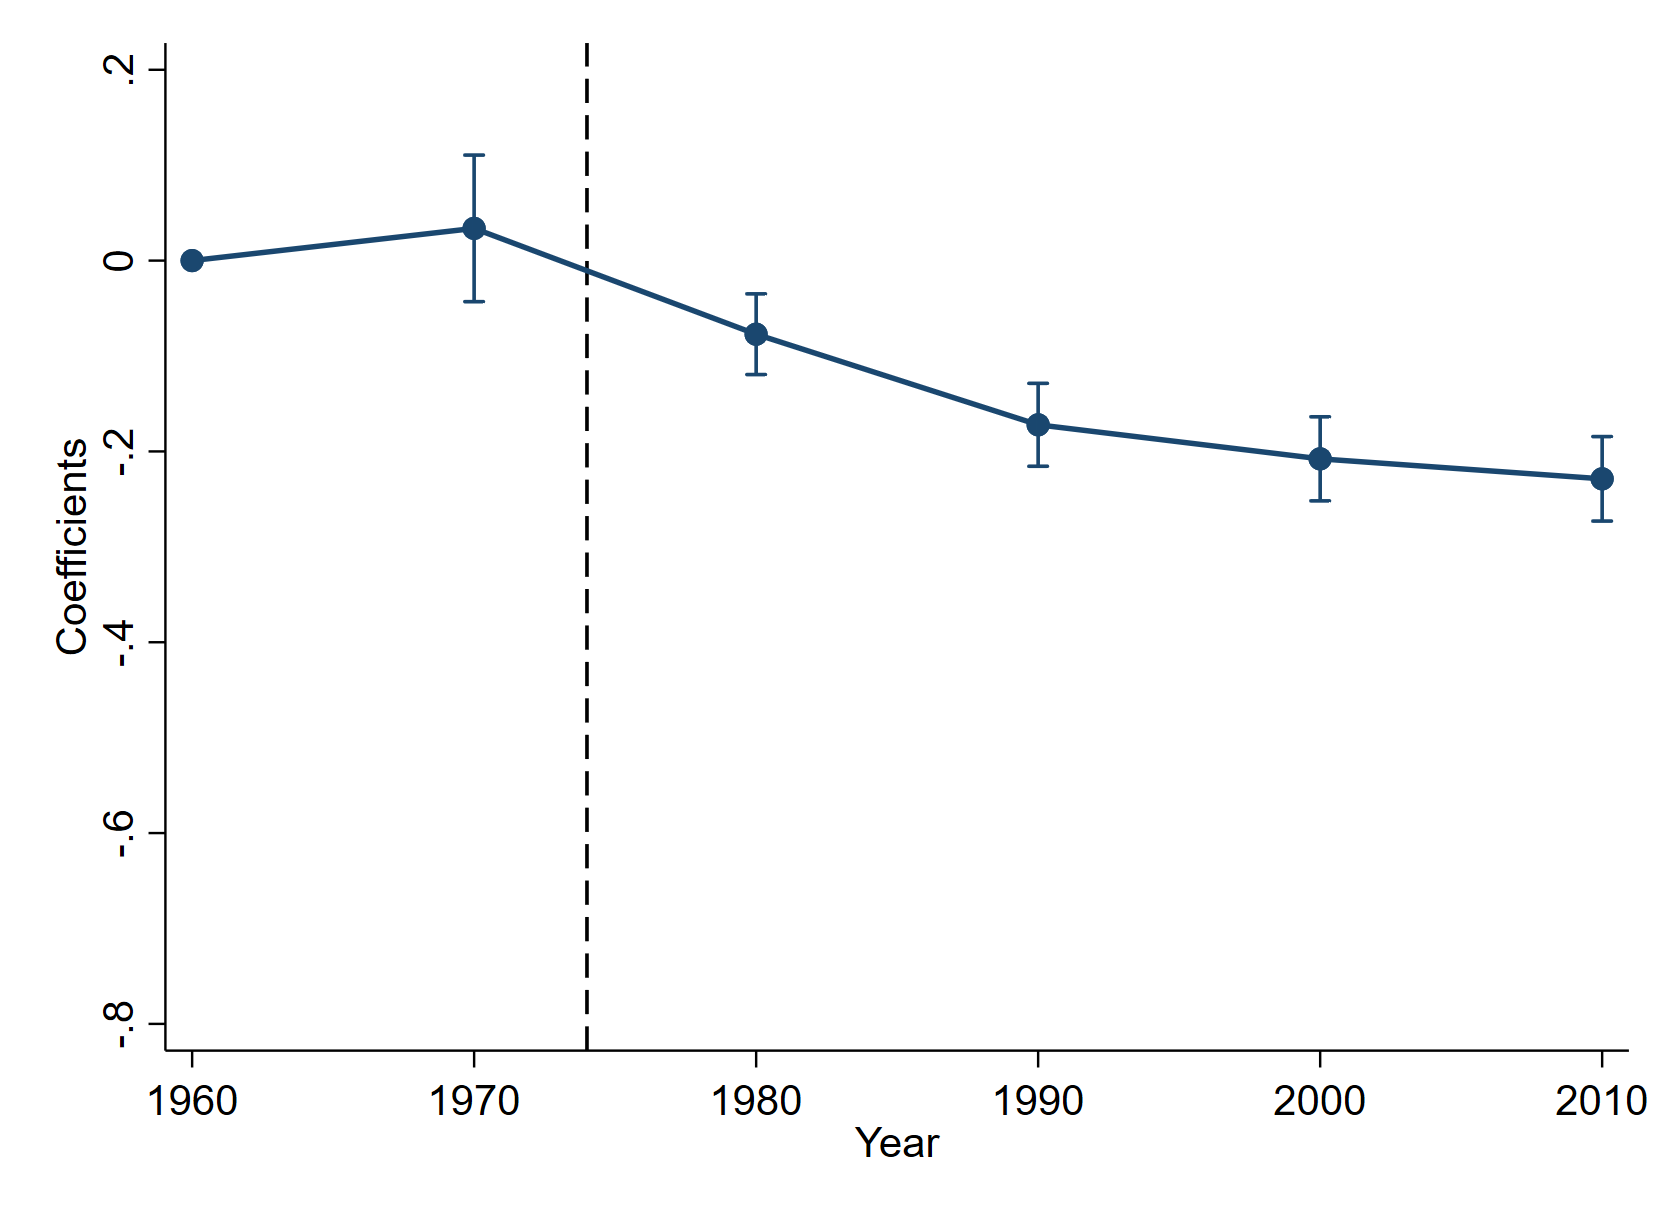
\includegraphics[width=\textwidth]{figures/road_imputation.png}
        \label{road_imputation}
    \end{subfigure}
    \begin{subfigure}{0.48\textwidth}
        \centering
        \caption{Callaway and Sant'Anna (2021) Estimator}
        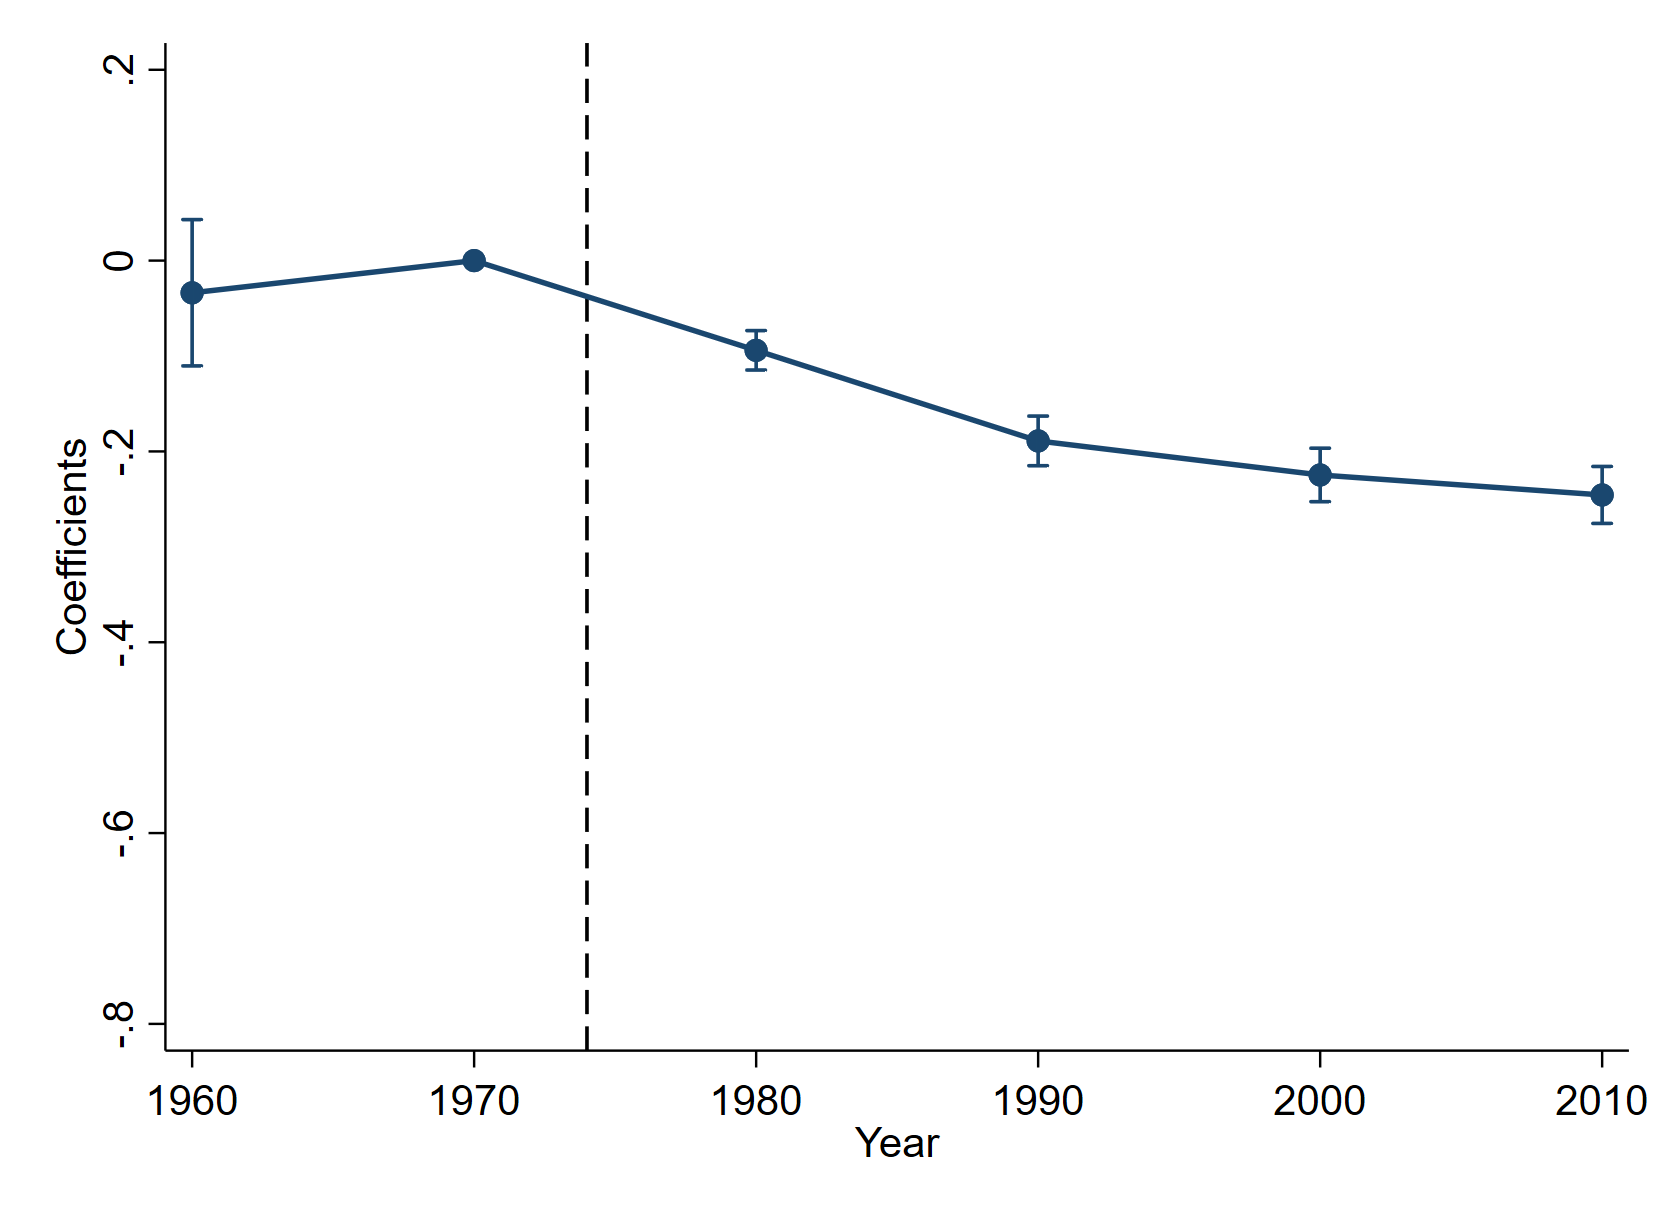
\includegraphics[width=\textwidth]{figures/road_csdid.png}
        \label{road_csdid}
    \end{subfigure}
\end{figure}
\clearpage

\begin{table}[p]\centering
\def\sym#1{\ifmmode^{#1}\else\(^{#1}\)\fi}
\begingroup
\renewcommand{\arraystretch}{1.3}
\caption{PPML Regressions on Agricultural Land Use, 1974-2010 \label{tab:ppml}}
\sbox{\tabbox}{%
\resizebox{\linewidth}{!}{
\begin{tabular}{l*{8}{c}}
\hline\hline
                    &\multicolumn{2}{c}{Total Cropland}         &\multicolumn{2}{c}{Sensitive}              &\multicolumn{2}{c}{Insensitive}            &\multicolumn{2}{c}{Pasture}                \\\cmidrule(lr){2-3}\cmidrule(lr){4-5}\cmidrule(lr){6-7}\cmidrule(lr){8-9}
                    &\multicolumn{1}{c}{(1)}         &\multicolumn{1}{c}{(2)}         &\multicolumn{1}{c}{(3)}         &\multicolumn{1}{c}{(4)}         &\multicolumn{1}{c}{(5)}         &\multicolumn{1}{c}{(6)}         &\multicolumn{1}{c}{(7)}         &\multicolumn{1}{c}{(8)}         \\
                    &        PPML         &Reduced Form         &        PPML         &Reduced Form         &        PPML         &Reduced Form         &        PPML         &Reduced Form         \\
\hline
$\Delta Log Travel Time$&       0.349         &                     &       1.462\sym{*}  &                     &      -0.104         &                     &      -0.113         &                     \\
                    &     (0.479)         &                     &     (0.776)         &                     &     (0.274)         &                     &     (0.291)         &                     \\
PIN-Induced Reduction&                     &       0.208         &                     &       1.138\sym{**} &                     &       0.611\sym{**} &                     &      -0.013         \\
                    &                     &     (0.272)         &                     &     (0.572)         &                     &     (0.259)         &                     &     (0.156)         \\
\hline
State FE            &         Yes         &         Yes         &         Yes         &         Yes         &         Yes         &         Yes         &         Yes         &         Yes         \\
Initial level of outcome&         Yes         &         Yes         &         Yes         &         Yes         &         Yes         &         Yes         &         Yes         &         Yes         \\
Observations        &         528         &         528         &         481         &         481         &         502         &         502         &         528         &         528         \\
\hline\hline
\end{tabular}}
}
\usebox{\tabbox}
\begin{minipage}{\wd\tabbox}
    \vspace{0.1cm}
    {\footnotesize \sloppy \textit{Notes: } Each observation is a micro-region. Columns labelled PPML use the actual change in log travel time; columns labelled Reduced Form replace it with the PIN-induced reduction. The initial level of the outcome enters as an offset, so the dependent variable is a growth ratio. Standard errors clustered at the state level are reported in parentheses. ***,**,* imply significance at the 1\%, 5\%, and 10\% levels, respectively.}
\end{minipage}
\endgroup
\end{table}

\clearpage

\begin{table}[p]\centering
\def\sym#1{\ifmmode^{#1}\else\(^{#1}\)\fi}
\begingroup
\renewcommand{\arraystretch}{1.3}
\caption{Alternative Measures of Employment and Agricultural Output \label{tab:altmeasures}}
\sbox{\tabbox}{%
\resizebox{\linewidth}{!}{
\begin{tabular}{l*{10}{c}}
\hline
\hline
&\multicolumn{2}{c}{Rural Employment}       &\multicolumn{2}{c}{Urban Employment}       &\multicolumn{2}{c}{Sensitive}              &\multicolumn{2}{c}{Insensitive}            &\multicolumn{2}{c}{Pasture}                \\\cmidrule(lr){2-3}\cmidrule(lr){4-5}\cmidrule(lr){6-7}\cmidrule(lr){8-9}\cmidrule(lr){10-11}
&\multicolumn{1}{c}{(1)}         &\multicolumn{1}{c}{(2)}         &\multicolumn{1}{c}{(3)}         &\multicolumn{1}{c}{(4)}         &\multicolumn{1}{c}{(5)}         &\multicolumn{1}{c}{(6)}         &\multicolumn{1}{c}{(7)}         &\multicolumn{1}{c}{(8)}         &\multicolumn{1}{c}{(9)}         &\multicolumn{1}{c}{(10)}         \\
&         OLS         &          IV         &         OLS         &          IV         &         OLS         &          IV         &         OLS         &          IV         &         OLS         &          IV         \\
\hline
\multicolumn{10}{l}{\textbf{\textit{Panel A: Baseline controlling only for the initial value of the outcome}}} \\
$\Delta Log Travel Time$&       0.407\sym{*}  &       0.858\sym{***}&       0.428\sym{*}  &       1.013\sym{***}&       5.893\sym{***}&       7.573\sym{***}&      -0.175         &       1.583         &       1.191\sym{***}&       2.456\sym{***}\\
&     (0.218)         &     (0.313)         &     (0.220)         &     (0.235)         &     (2.025)         &     (2.383)         &     (0.828)         &     (1.076)         &     (0.327)         &     (0.663)         \\
Observations        &         531         &         531         &         531         &         531         &         531         &         531         &         531         &         531         &         531         &         531         \\
First-stage F stat  &                     &      84.433         &                     &      80.739         &                     &      79.841         &                     &      79.235         &                     &      88.191         \\
\hline
\multicolumn{10}{l}{\linebreak \textbf{\textit{Panel B: Panel (A) including state fixed effects}}} \\
$\Delta Log Travel Time$&       0.165         &       0.257         &       0.064         &       0.450\sym{**} &       3.372\sym{**} &       5.086\sym{**} &       0.522         &       1.819         &       0.265         &       0.958         \\
&     (0.132)         &     (0.196)         &     (0.131)         &     (0.179)         &     (1.323)         &     (1.901)         &     (0.655)         &     (1.132)         &     (0.421)         &     (0.655)         \\
Observations        &         528         &         528         &         528         &         528         &         528         &         528         &         528         &         528         &         528         &         528         \\
First-stage F stat  &                     &      64.766         &                     &      64.271         &                     &      63.212         &                     &      61.665         &                     &      64.284         \\
\hline
\multicolumn{10}{l}{\linebreak \textbf{\textit{Panel C: Panel (B) including covariates for additional geographical traits}}} \\
$\Delta Log Travel Time$&       0.038         &       0.116         &      -0.051         &       0.346\sym{*}  &       2.544\sym{*}  &       3.968\sym{*}  &       0.015         &       1.187         &      -0.066         &       0.465         \\
&     (0.154)         &     (0.168)         &     (0.174)         &     (0.184)         &     (1.319)         &     (2.107)         &     (0.644)         &     (1.148)         &     (0.359)         &     (0.495)         \\
Observations        &         528         &         528         &         528         &         528         &         528         &         528         &         528         &         528         &         528         &         528         \\
First-stage F stat  &                     &      58.387         &                     &      57.894         &                     &      58.078         &                     &      56.366         &                     &      52.091         \\
\hline\hline
\end{tabular}}
}
\usebox{\tabbox}
\begin{minipage}{\wd\tabbox}
    \vspace{0.1cm}
    {\footnotesize \sloppy \textit{Notes: } Each observation is a micro-region. Log change in travel time on roads is instrumented by the change in travel times on the predicted road network. The predicted road network is created by geo-referencing the PNV National Transportation Plan in 1973. The Kleibergen-Paap F-statistic (First-stage F stat) for weak identification is reported for IV estimates. Standard errors clustered at the state level are reported in parentheses. Employment is the economically active population. The crop columns measure production rather than harvested area; IBGE reports no output quantity for cattle, so the pasture column measures the herd and is identical to its counterpart in the land-use table. ***,**,* imply significance at the 1\%, 5\%, and 10\% levels, respectively.}
\end{minipage}
\endgroup
\end{table}

\clearpage

\begin{table}[p]\centering
\def\sym#1{\ifmmode^{#1}\else\(^{#1}\)\fi}
\begingroup
\renewcommand{\arraystretch}{1.3}
\caption{Long-difference estimates using alternative Sample Choices \label{tab:altsamples}}
\sbox{\tabbox}{%
\resizebox{\linewidth}{!}{
\begin{tabular}{l*{8}{c}}
\hline
\hline
&\multicolumn{1}{c}{(1)}         &\multicolumn{1}{c}{(2)}         &\multicolumn{1}{c}{(3)}         &\multicolumn{1}{c}{(4)}         &\multicolumn{1}{c}{(5)}         &\multicolumn{1}{c}{(6)}         &\multicolumn{1}{c}{(7)}         &\multicolumn{1}{c}{(8)}         \\
&         GDP         &  Population         &Urban Population         &Urban Employment Share         &Total Cropland         &   Sensitive         & Insensitive         &     Pasture         \\
\hline
\multicolumn{8}{l}{\textbf{\textit{Panel A: Micro-regions}}} \\
$\Delta Log Travel Time$&       0.272         &       0.076         &       0.329\sym{**} &       0.048         &      -0.035         &       3.732\sym{*}  &       1.050         &       0.465         \\
&     (0.287)         &     (0.230)         &     (0.148)         &     (0.040)         &     (0.591)         &     (1.928)         &     (1.239)         &     (0.495)         \\
Observations        &         528         &         528         &         528         &         528         &         528         &         528         &         528         &         528         \\
State FE            &         Yes         &         Yes         &         Yes         &         Yes         &         Yes         &         Yes         &         Yes         &         Yes         \\
Initial level of outcome&         Yes         &         Yes         &         Yes         &         Yes         &         Yes         &         Yes         &         Yes         &         Yes         \\
Geographical Characteristics&         Yes         &         Yes         &         Yes         &         Yes         &         Yes         &         Yes         &         Yes         &         Yes         \\
\hline
\multicolumn{8}{l}{\linebreak \textbf{\textit{Panel B: Micro-regions excluding the Amazon}}} \\
$\Delta Log Travel Time$&       0.128         &      -0.024         &       0.269\sym{*}  &       0.039         &      -0.467         &       4.059\sym{*}  &       0.163         &      -0.185         \\
&     (0.292)         &     (0.237)         &     (0.146)         &     (0.043)         &     (0.562)         &     (2.138)         &     (0.966)         &     (0.265)         \\
Observations        &         490         &         490         &         490         &         490         &         490         &         490         &         490         &         490         \\
State FE            &         Yes         &         Yes         &         Yes         &         Yes         &         Yes         &         Yes         &         Yes         &         Yes         \\
Initial level of outcome&         Yes         &         Yes         &         Yes         &         Yes         &         Yes         &         Yes         &         Yes         &         Yes         \\
Geographical Characteristics&         Yes         &         Yes         &         Yes         &         Yes         &         Yes         &         Yes         &         Yes         &         Yes         \\
\hline
\multicolumn{8}{l}{\linebreak \textbf{\textit{Panel C: Meso-regions}}} \\
$\Delta Log Travel Time$&       0.097         &       0.097         &       0.225         &       0.034         &       0.393         &       2.717         &       1.194         &       0.506         \\
&     (0.611)         &     (0.310)         &     (0.335)         &     (0.085)         &     (0.709)         &     (2.096)         &     (1.174)         &     (0.600)         \\
Observations        &         132         &         132         &         132         &         132         &         132         &         132         &         132         &         132         \\
State FE            &         Yes         &         Yes         &         Yes         &         Yes         &         Yes         &         Yes         &         Yes         &         Yes         \\
Initial level of outcome&         Yes         &         Yes         &         Yes         &         Yes         &         Yes         &         Yes         &         Yes         &         Yes         \\
Geographical Characteristics&         Yes         &         Yes         &         Yes         &         Yes         &         Yes         &         Yes         &         Yes         &         Yes         \\
\hline\hline
\end{tabular}}
}
\usebox{\tabbox}
\begin{minipage}{\wd\tabbox}
    \vspace{0.1cm}
    {\footnotesize \sloppy \textit{Notes: } Each observation is a micro-region. Log change in travel time on roads is instrumented by the change in travel times on the predicted road network. The predicted road network is created by geo-referencing the PNV National Transportation Plan in 1973. The Kleibergen-Paap F-statistic (First-stage F stat) for weak identification is reported for IV estimates. Standard errors clustered at the state level are reported in parentheses. Panel B drops micro-regions in the Legal Amazon. Panel C aggregates to meso-regions. ***,**,* imply significance at the 1\%, 5\%, and 10\% levels, respectively.}
\end{minipage}
\endgroup
\end{table}

\clearpage


\newpage
\section*{Appendix}

\appendix
\section{Derivations and Proofs}
\label{app:derivations}

\subsection{Aggregate Agricultural Productivity}
\label{app:zA}

This section derives the aggregate revenue productivity of agriculture in equation
\eqref{eq:zA} and the land shares in equation \eqref{eq:landshare}. Consider a plot $j$ in
location $\ell$ allocated to agricultural good $g$. The landowner chooses employment density
to solve the inner problem in equation \eqref{eq:landalloc}, whose first-order condition gives
\begin{equation}
n_{g\ell j}=\left(\frac{(1-\alpha_A)P_{g\ell}z_{g\ell j}}{w_\ell}\right)^{\frac{1}{\alpha_A}}.
\label{eq:n_plot}
\end{equation}
Under the Cobb-Douglas technology land collects the share $\alpha_A$ of revenue, so that
$r_{g\ell j}=\alpha_A P_{g\ell}q_{g\ell j}$. Substituting equation \eqref{eq:n_plot} expresses
the rent as a function of the productivity draw,
\begin{equation}
r_{g\ell j}=\kappa_A\, w_\ell^{-\frac{1-\alpha_A}{\alpha_A}}
\left(P_{g\ell}z_{g\ell j}\right)^{\frac{1}{\alpha_A}},
\qquad
\kappa_A \equiv \alpha_A(1-\alpha_A)^{\frac{1-\alpha_A}{\alpha_A}}.
\label{eq:rent_plot}
\end{equation}
Because equation \eqref{eq:rent_plot} is a strictly increasing power transformation of
$z_{g\ell j}$, inverting it and applying the Fr\'echet distribution \eqref{eq:frechet_prod}
gives
\begin{equation}
\Pr\!\left[r_{g\ell j}\le r\right]=\exp\!\left(-A_{g\ell}\,r^{-\alpha_A\theta}\right),
\qquad
A_{g\ell}\equiv T_{g\ell}\,\kappa_A^{\alpha_A\theta}\,
w_\ell^{-\theta(1-\alpha_A)}P_{g\ell}^{\theta},
\label{eq:rent_frechet}
\end{equation}
so plot-level rents are themselves Fr\'echet, with shape parameter $\alpha_A\theta$.

The plot is allocated to the good delivering the highest rent. Since the draws are independent across goods,
\[
\Pr\!\left[r_{\ell j}\le r\right]=\prod_{g=1}^G \Pr\!\left[r_{g\ell j}\le r\right]
=\exp\!\left(-\Big(\sum_{g=1}^G A_{g\ell}\Big) r^{-\alpha_A\theta}\right),
\]
so the maximized rent is Fr\'echet with scale $\sum_g A_{g\ell}$ and the same shape parameter. With a continuum of plots, the share of agricultural land devoted to good $g$ equals the probability that $g$ attains the maximum, $l_{g\ell}=A_{g\ell}/\sum_h A_{h\ell}$. The factors
$\kappa_A^{\alpha_A\theta}$ and $w_\ell^{-\theta(1-\alpha_A)}$ are common across goods and cancel, which gives equation \eqref{eq:landshare}.


Expected agricultural rent per plot is the mean of that Fr\'echet distribution, which is finite
when $\alpha_A\theta>1$:
\begin{equation}
r_{A\ell}=\mathbb{E}\left[r_{\ell j}\right]
=\Gamma\!\left(\frac{\alpha_A\theta-1}{\alpha_A\theta}\right)
\kappa_A\, w_\ell^{-\frac{1-\alpha_A}{\alpha_A}}
\left(\sum_{g=1}^G T_{g\ell}P_{g\ell}^{\theta}\right)^{\frac{1}{\alpha_A\theta}}.
\label{eq:rentA}
\end{equation}
Define $z_{A\ell}$ as the revenue productivity of a hypothetical single-good agricultural
sector that generates the same expected rent. Evaluating equation \eqref{eq:rent_plot} with
$P_{g\ell}z_{g\ell j}$ replaced by $z_{A\ell}$ gives
$r_{A\ell}=\kappa_A w_\ell^{-(1-\alpha_A)/\alpha_A}z_{A\ell}^{1/\alpha_A}$; equating this with
equation \eqref{eq:rentA} and raising both sides to the power $\alpha_A$ yields equation
\eqref{eq:zA}. The common factors drop out again, so $z_{A\ell}$ depends on the disaggregated
goods only through the index $\sum_g T_{g\ell}P_{g\ell}^\theta$.

Log-differentiating equation \eqref{eq:zA} with respect to $\ln P_{g\ell}$ gives
\[
\frac{\partial \ln z_{A\ell}}{\partial \ln P_{g\ell}}
=\frac{1}{\theta}\cdot
\frac{\theta\,T_{g\ell}P_{g\ell}^{\theta}}{\sum_h T_{h\ell}P_{h\ell}^{\theta}}
=l_{g\ell},
\]
so the land shares are also the elasticities of aggregate revenue productivity with respect to
the disaggregated prices.

\subsection{The Local Equilibrium}
\label{app:localeq}

This section derives the closed-form solutions for population density in equation \eqref{eq:density} and the agricultural labor share in equation \eqref{eq:nuA}. Let $\lambda_{N\ell}=L_{N\ell}/L_\ell$ and $\lambda_{A\ell}=L_{A\ell}/L_\ell$ denote the non-tradable and agricultural land shares, so that $\lambda_{N\ell}+\lambda_{A\ell}=1$.

Non-tradable market clearing requires expenditure on non-tradables per unit of land to equal non-tradable revenue per unit of land. Land earns the Cobb-Douglas share $\alpha_N$ of non-tradable revenue and both active sectors pay the common rent $r_\ell=w_\ell/\omega_\ell$, so revenue per unit of non-tradable land is $P_{N\ell}q_{N\ell}=r_\ell/\alpha_N=w_\ell/(\alpha_N\omega_\ell)$, while expenditure per unit of land is $(1-s_{T\ell})y_\ell$ with $y_\ell$ from equation \eqref{eq:income}. Equating the two,
\begin{equation}
    \lambda_{N\ell}\frac{w_\ell}{\alpha_N\omega_\ell}=(1-s_{T\ell})w_\ell\left(n_\ell+\omega_\ell^{-1}\right),\qquad\text{so}\qquad\lambda_{N\ell}= \alpha_N (1-s_{T\ell}) \omega_\ell \left(n_\ell+\omega_\ell^{-1}\right).
    \label{eq:lambdaN}
\end{equation}
Multiplying $\lambda_{N\ell}$ by non-tradable employment density $n_{N\ell}=\frac{1-\alpha_N}{\alpha_N}\omega_\ell^{-1}$ from equation \eqref{eq:n} gives non-tradable employment per unit of land area,
\begin{equation}
    \frac{N_{N\ell}}{L_\ell} = \lambda_{N\ell}n_{N\ell}= (1-\alpha_N)(1-s_{T\ell})\left(n_\ell+\omega_\ell^{-1}\right).
    \label{eq:Nlabor}
\end{equation}
Using $\lambda_{N\ell}+\lambda_{A\ell}=1$ together with equation \eqref{eq:lambdaN}, the land market clearing condition can be written as
\begin{equation}
    \alpha_N(1-s_{T\ell})\left(n_\ell+\frac{1}{\omega_\ell}\right)
+ \frac{\lambda_{A\ell}}{\omega_\ell}= \frac{1}{\omega_\ell},
\label{eq:land_clearing}
\end{equation}
and, combining profit maximization in agriculture from equation \eqref{eq:n}, the labor market clearing condition as
\begin{equation}
    (1-\alpha_N)(1-s_{T\ell})\left(n_\ell+\frac{1}{\omega_\ell}\right)
+ \frac{1-\alpha_A}{\alpha_A}\frac{\lambda_{A\ell}}{\omega_\ell}= n_\ell,
\label{eq:labor_clearing}
\end{equation}
Adding up equations \eqref{eq:land_clearing} and \eqref{eq:labor_clearing} gives
\begin{equation}
    \lambda_{A\ell}=\alpha_A s_{T\ell}(1+\omega_\ell n_\ell).
    \label{eq:lambda}
\end{equation}
Substituting equation \eqref{eq:lambda} back into equation \eqref{eq:land_clearing} and solving for $n_\ell$ yields equation \eqref{eq:density} in the main text. Finally, the agricultural labor share satisfies $\nu_{A\ell}=\frac{N_{A\ell}/L_\ell}{n_\ell}$ with $N_{A\ell}/L_\ell = n_\ell - N_{N\ell}/L_\ell$; combining equations \eqref{eq:Nlabor}, \eqref{eq:lambda}, and \eqref{eq:density} yields equation \eqref{eq:nuA}.

\subsection{Sufficient Statistics}
\label{app:suff}

Zero profits in the two active sectors require
\begin{equation}
    z_{A\ell}=w_\ell^{1-\alpha_A}r_\ell^{\alpha_A},\qquad P_{N\ell}z_{N\ell}=w_\ell^{1-\alpha_N}r_\ell^{\alpha_N},
    \label{eq:zeroprofit}
\end{equation}
where agriculture is treated as a single sector with revenue productivity $z_{A\ell}$ by equation \eqref{eq:zA}. Substituting $r_\ell=w_\ell/\omega_\ell$ into the first condition gives equations \eqref{eq:wage} and \eqref{eq:rent}, and dividing the second condition by the first gives equation \eqref{eq:PN}. Expressing the common component of utility in equation \eqref{eq:utility} in the indirect utility form $u_\ell=w_\ell/E_\ell$ together with equation \eqref{eq:wage} gives
\begin{equation}
\frac{E_{T\ell}}{E_\ell}
=
\frac{u_\ell}{\omega_\ell^{\alpha_A}\tilde z_{A\ell}},
\qquad
\frac{P_{N\ell}}{E_\ell}
=
\frac{u_\ell}{\omega_\ell^{\alpha_N}z_{N\ell}},
\label{eq:ETE}
\end{equation}
and therefore, using equation \eqref{eq:sT_def},
\begin{equation}
s_{T\ell}
=
\beta_T
\left(
\frac{u_\ell}{\tilde z_{A\ell} \omega_\ell^{\alpha_A}}
\right)^{1-\sigma}.
\label{eq:sT}
\end{equation}
Dividing the price index \eqref{eq:E} through by $E_\ell$ gives $1=\beta_T\left(E_{T\ell}/E_\ell\right)^{1-\sigma}+(1-\beta_T)\left(P_{N\ell}/E_\ell\right)^{1-\sigma}$; substituting equation \eqref{eq:ETE} and rearranging yields equation \eqref{eq:omega_eq} in the main text.

\subsection{Proof of Lemma \texorpdfstring{\ref{lem:zad}}{1}}
\label{app:proof_zad}

\noindent\textbf{Lemma \ref{lem:zad}} (Trade costs and adjusted agricultural
productivity)\textbf{.} \emph{Suppose location $\ell$ imports manufactures and its agricultural
trade position satisfies}
\[
\sum_{g=1}^G \left(l_{g\ell}-\gamma_g\right)\tau_g + (1-\gamma_A)\tau_M \;>\; 0.
\]
\emph{Then}
\[
\frac{d \ln \tilde z_{A\ell}}{d t_\ell}
= -\Big[\sum_{g=1}^G \left(l_{g\ell}-\gamma_g\right)\tau_g + (1-\gamma_A)\tau_M\Big] < 0,
\]
\emph{so a reduction in travel time strictly raises adjusted agricultural
productivity.}\medskip

\begin{proof}
By the elasticity result following equation \eqref{eq:landshare} and the no-arbitrage prices $P_{g\ell}=P_g^\ast e^{-\tau_g t_\ell}$, $d\ln z_{A\ell}/dt_\ell = -\sum_g l_{g\ell}\tau_g$. Log-differentiating the tradables price index \eqref{eq:ET} with $P_{M\ell}=P_M^\ast e^{\tau_M t_\ell}$ gives $d\ln E_{T\ell}/dt_\ell = -\sum_g \gamma_g\tau_g + (1-\gamma_A)\tau_M$. Subtracting the second expression from the first and using $\tilde z_{A\ell}=z_{A\ell}/E_{T\ell}$ yields \eqref{eq:zad_t}. This is the specialization to $\delta_{g(\ell,\ell^\ast)}=e^{\tau_g t_\ell}$ of the decomposition in Fajgelbaum and Redding (2022, eqs.~35--37), in which $\hat{\tilde z}_{A\ell}=\hat z_{A\ell}-\hat E_{T\ell}$ with $\hat z_{A\ell}=\sum_g l_{g\ell}[\hat T_{g\ell}/\theta+\hat P_g^\ast-\hat\delta_g]$ and $\hat E_{T\ell}=(1-\gamma_A)[\hat P_M^\ast+\hat\delta_M]+\sum_g\gamma_g[\hat P_g^\ast-\hat\delta_g]$; holding technology and world prices fixed leaves the weights $l_{g\ell}-\gamma_g$ on the agricultural trade costs and $-(1-\gamma_A)$ on the manufacturing trade cost. The sign is strictly negative by condition \eqref{eq:net_export}.
\end{proof}

\subsection{Proof of Proposition \texorpdfstring{\ref{prop:bs}}{1}}
\label{app:proof_bs}

\noindent\textbf{Proposition \ref{prop:bs}} (Spatial Balassa-Samuelson effect)\textbf{.}
\emph{Assume agricultural and non-tradable goods are complements ($\sigma<1$), agriculture is
land-intensive relative to non-tradables ($\alpha_A>\alpha_N$), population is mobile ($\epsilon$
sufficiently large), and condition \eqref{eq:net_export} holds. Then a location with lower
travel time $t_\ell$ has (i) higher adjusted agricultural productivity $\tilde z_{A\ell}$;
(ii) a lower tradable expenditure share $s_{T\ell}$; (iii) higher population density $n_\ell$;
(iv) a lower agricultural employment share $\nu_{A\ell}$; (v) a lower wage-rental ratio
$\omega_\ell$; and (vi) higher GDP per unit of land $y_\ell$ in equation
\eqref{eq:income}.}\medskip

\begin{proof}
With perfect mobility, $u_\ell = u^\ast$ for all populated locations. Define $a_\ell \equiv \tilde z_{A\ell}\,\omega_\ell^{\alpha_A}$ and $v_\ell \equiv z_{N\ell}\,\omega_\ell^{\alpha_N}$, so that equation \eqref{eq:omega_eq} reads
\[
\beta_T\, a_\ell^{\sigma-1} + (1-\beta_T)\, v_\ell^{\sigma-1} = (u^\ast)^{\sigma-1}.
\]
(i) Since $\sigma<1$, the left-hand side is strictly decreasing in both $\omega_\ell$ and $\tilde z_{A\ell}$; and since $u^\ast$ is common to all locations, a location with higher $\tilde z_{A\ell}$ therefore has a lower $\omega_\ell$. (ii) A lower $\omega_\ell$ with $z_{N\ell}$ fixed lowers $v_\ell$ and hence raises $v_\ell^{\sigma-1}$; the identity then requires $a_\ell^{\sigma-1}$ to fall, i.e., $a_\ell$ to rise. By equation \eqref{eq:sT}, $s_{T\ell}=\beta_T (u^\ast/a_\ell)^{1-\sigma}$ falls. (iii) In equation \eqref{eq:density}, the term in parentheses is positive and strictly decreasing in $s_{T\ell}$ given $\alpha_A>\alpha_N$, so a lower $s_{T\ell}$ raises it; combined with a lower $\omega_\ell$, population density $n_\ell$ rises. (iv) In equation \eqref{eq:nuA}, the numerator is increasing and the denominator decreasing in $s_{T\ell}$, so $\nu_{A\ell}$ is strictly increasing in $s_{T\ell}$ and therefore falls.
(v) Established in (i). (vi) Write $y_\ell = r_\ell (1+\omega_\ell n_\ell)$. From equation \eqref{eq:rent}, $r_\ell = z_{A\ell}\,\omega_\ell^{\alpha_A-1}$: a lower $t_\ell$ raises $z_{A\ell}$ (Lemma \ref{lem:zad}) and lowers $\omega_\ell$ by (i), and since $\alpha_A-1<0$ both movements raise $r_\ell$. From equation \eqref{eq:density}, $\omega_\ell n_\ell = \left[\alpha_N+(\alpha_A-\alpha_N)s_{T\ell}\right]^{-1}-1$ rises as $s_{T\ell}$ falls. Hence $y_\ell$ rises.
\end{proof}



\subsection{Proof of Proposition \texorpdfstring{\ref{prop:specialization}}{2}}
\label{app:proof_spec}

\noindent\textbf{Proposition \ref{prop:specialization}} (Specialization within
agriculture)\textbf{.} \emph{Locations with shorter travel time to the international gateway
allocate relatively more land to transport-cost-sensitive agricultural goods: for every good
$g$,}
\[
\frac{d \ln l_{g\ell}}{d t_\ell}
= -\theta \left(\tau_g - \bar{\tau}_\ell\right),
\qquad
\bar{\tau}_\ell \equiv \sum_{h=1}^G l_{h\ell} \tau_h,
\]
\emph{where $\bar{\tau}_\ell$ is the land-share-weighted average transport-cost sensitivity in
location $\ell$. As travel time falls, the land share rises for goods with above-average
transport-cost sensitivity ($\tau_g > \bar{\tau}_\ell$) and falls for goods with below-average
sensitivity.}\medskip

\begin{proof}
Substituting the no-arbitrage prices $P_{g\ell}=P_g^\ast/\delta_{g(\ell,\ell^*)}=P_g^\ast e^{-\tau_g t_\ell}$ into the land shares \eqref{eq:landshare}, define the good-specific competitiveness term
\[
A_{g\ell}(t_\ell)\equiv T_{g\ell}P_{g\ell}(t_\ell)^\theta
= T_{g\ell}(P_g^*)^\theta e^{-\theta\tau_g t_\ell},
\qquad
l_{g\ell}=\frac{A_{g\ell}}{\sum_h A_{h\ell}}.
\]
Then $d\ln A_{g\ell}/dt_\ell = -\theta\tau_g$ and $d \ln \left(\sum_h A_{h\ell}\right)/dt_\ell = -\theta\sum_h l_{h\ell}\tau_h = -\theta\bar{\tau}_\ell$; subtracting the second expression from the first yields \eqref{eq:landshare_d}.
\end{proof}

\subsection{Proof of Proposition \texorpdfstring{\ref{prop:complementarity}}{3}}
\label{app:proof_comp}

\noindent\textbf{Proposition \ref{prop:complementarity}} (The trade regime and the travel-time
elasticity)\textbf{.} \emph{Consider a change in the trade regime $\{d\ln\chi_g\}_{g=1}^G$,
holding $\chi_M$ fixed and assuming condition \eqref{eq:net_export} continues to hold. Then:
(i) if the wedge is uniform, the land shares \eqref{eq:landshare} are invariant to $\chi$, so
$\ln \tilde z_{A\ell}$ is additively separable in $\ln\chi$ and $t_\ell$ and
$\partial^2 \ln\tilde z_{A\ell}/\partial\ln\chi\,\partial t_\ell = 0$; (ii) if the wedge varies
across goods, the land shares respond as
$d \ln l_{g\ell} = \theta( d\ln\chi_g - \sum_{h} l_{h\ell}\, d\ln\chi_h )$ and the travel-time
derivative \eqref{eq:zad_t} changes by
$-\,\theta\,\mathrm{Cov}_{\,l_\ell}(\tau_g,\, d\ln\chi_g)$, a land-share-weighted
covariance.}\medskip

\begin{proof}
(i) With a uniform wedge, equation \eqref{eq:prices_chi} gives $P_{g\ell}^\theta=\chi^\theta (P_g^\ast)^\theta e^{-\theta\tau_g t_\ell}$, so the factor $\chi^\theta$ appears in both the numerator and the denominator of \eqref{eq:landshare} and cancels: $l_{g\ell}$ is invariant to $\chi$. Hence, by \eqref{eq:zA}, $\ln z_{A\ell}$ shifts by $\ln\chi$; by \eqref{eq:ET}, $\ln E_{T\ell}$ shifts by $\gamma_A\ln\chi-(1-\gamma_A)\ln\chi=(2\gamma_A-1)\ln\chi$; and therefore $\ln \tilde z_{A\ell}$ shifts by $2(1-\gamma_A)\ln\chi>0$, uniformly across locations. The travel-time derivative \eqref{eq:zad_t} depends on $\chi$ only through the land shares and is therefore unchanged, giving $\partial^2 \ln\tilde z_{A\ell}/\partial\ln\chi\,\partial t_\ell = 0$.

(ii) With good-specific wedges, write $A_{g\ell}=T_{g\ell}(\chi_g P_g^\ast)^\theta e^{-\theta\tau_g t_\ell}$ so that $l_{g\ell}=A_{g\ell}/\sum_h A_{h\ell}$. Then $\partial\ln A_{g\ell}/\partial\ln\chi_g=\theta$ and $\partial\ln\left(\sum_h A_{h\ell}\right)/\partial\ln\chi_g=\theta l_{g\ell}$, so $\partial \ln l_{g\ell}/\partial\ln\chi_g=\theta(1-l_{g\ell})$ and $\partial \ln l_{g\ell}/\partial\ln\chi_h=-\theta l_{h\ell}$ for $h\neq g$. Totalling over the wedge changes gives the stated expression for $d\ln l_{g\ell}$. Since $\gamma_g$, $\gamma_A$ and $\tau_M$ are fixed, differentiating \eqref{eq:zad_t} gives $d(d \ln \tilde z_{A\ell}/dt_\ell) = -\sum_g \tau_g\, d l_{g\ell}$. Using $d l_{g\ell}=l_{g\ell}\,d\ln l_{g\ell}$ and the previous display,
\[
\sum_g \tau_g\, d l_{g\ell}
= \theta\left[\sum_g l_{g\ell}\tau_g\, d\ln\chi_g - \Big(\sum_g l_{g\ell}\tau_g\Big)\Big(\sum_h l_{h\ell}\, d\ln\chi_h\Big)\right]
= \theta\,\mathrm{Cov}_{\,l_\ell}\!\left(\tau_g, d\ln\chi_g\right),
\]
which is the stated expression. If $d\ln\chi_g$ is the same for all $g$ the covariance is zero, recovering part (i).
\end{proof}

\newpage
\section{Tables and Figures}
\label{app:tabfig}

\subsection{Product Classification}
\label{app:classification}

Table \ref{tab:classification} reports every traded crop with the two measured criteria behind its placement: the FAOSTAT export ratio, which determines traded status, and value per tonne computed from PAM production value divided by quantity in 2010, which proxies transport-cost sensitivity. The final column gives the share of micro-regions recording positive area in 1974. The value-per-tonne distribution has no crop between 1,400 and 2,692 R\$ per tonne, so the classification does not depend on where in that interval a threshold is drawn.


\begin{table}[htbp]\centering
\begingroup
\renewcommand{\arraystretch}{1.3}
\caption{Product Classification \label{tab:classification}}
\sbox{\tabbox}{%
\begin{tabular}{lccc}
\hline\hline
 & Export & Value per & Micro-regions \\
Crop & ratio & tonne (R\$) & growing, 1974 (\%) \\
\hline
\multicolumn{4}{l}{\emph{Transport-cost-sensitive}} \\
\quad Soybean & 0.99 & 543 & 34.2 \\
\quad Sisal & -- & 897 & 10.9 \\
\quad Castor & -- & 951 & 38.3 \\
\addlinespace \multicolumn{4}{l}{\emph{Transport-cost-insensitive}} \\
\quad Walnut & 0.08 & 2,692 & 3.4 \\
\quad Coffee & 0.69 & 3,983 & 52.8 \\
\quad Black pepper & 0.65 & 5,156 & 8.1 \\
\quad Cocoa & 0.26 & 5,226 & 7.9 \\
\quad Tobacco & 0.49 & 5,733 & 55.3 \\
\addlinespace \multicolumn{4}{l}{\emph{Excluded}} \\
\quad Sugarcane & 0.11 & 39 & 89.3 \\
\quad Orange & 0.32 & 332 & 94.2 \\
\quad Cotton (arboreal) & 0.10 & 869 & 21.4 \\
\quad Cashew & 0.92 & 1,085 & 0.0 \\
\quad Peanut & 0.30 & 1,094 & 60.0 \\
\quad Cotton (herbaceous) & 0.10 & 1,400 & 53.9 \\
\hline\hline
\end{tabular}
}
\usebox{\tabbox}
\begin{minipage}{\wd\tabbox}
    \vspace{0.1cm}
    {\footnotesize \sloppy \textit{Notes: } Value per tonne is national production value divided by quantity in 2010, from the Municipal Agricultural Production survey. The export ratio is the FAOSTAT mean ratio of exports to production; it is omitted for sisal and castor because their FAOSTAT export items do not match the production series. The final column is the share of micro-regions recording positive area in 1974.}
\end{minipage}
\endgroup
\end{table}


Sisal and castor carry no export ratio because their FAOSTAT export items do not match the production series; both are added to the traded set by hand, since Brazil exports them heavily. Cashew records no area in 1974, which is a collection gap rather than an absence, so it cannot enter a long difference beginning in that year. Coffee's prevalence of 52.8\% is why it is the insensitive crop reported in Table \ref{tab:descriptives}: cocoa, pepper and walnut are each present in under 9\% of micro-regions and are too rare to represent the group.



\clearpage

\subsection{Additional Figures}
\label{app:figures}

\begin{figure}[H]
    \centering
    \caption*{Appendix Figure 1: Evolution of Brazil’s federal highway system, 1960-2010}
    \begin{subfigure}{0.32\textwidth}
        \centering
        \caption{1960}
        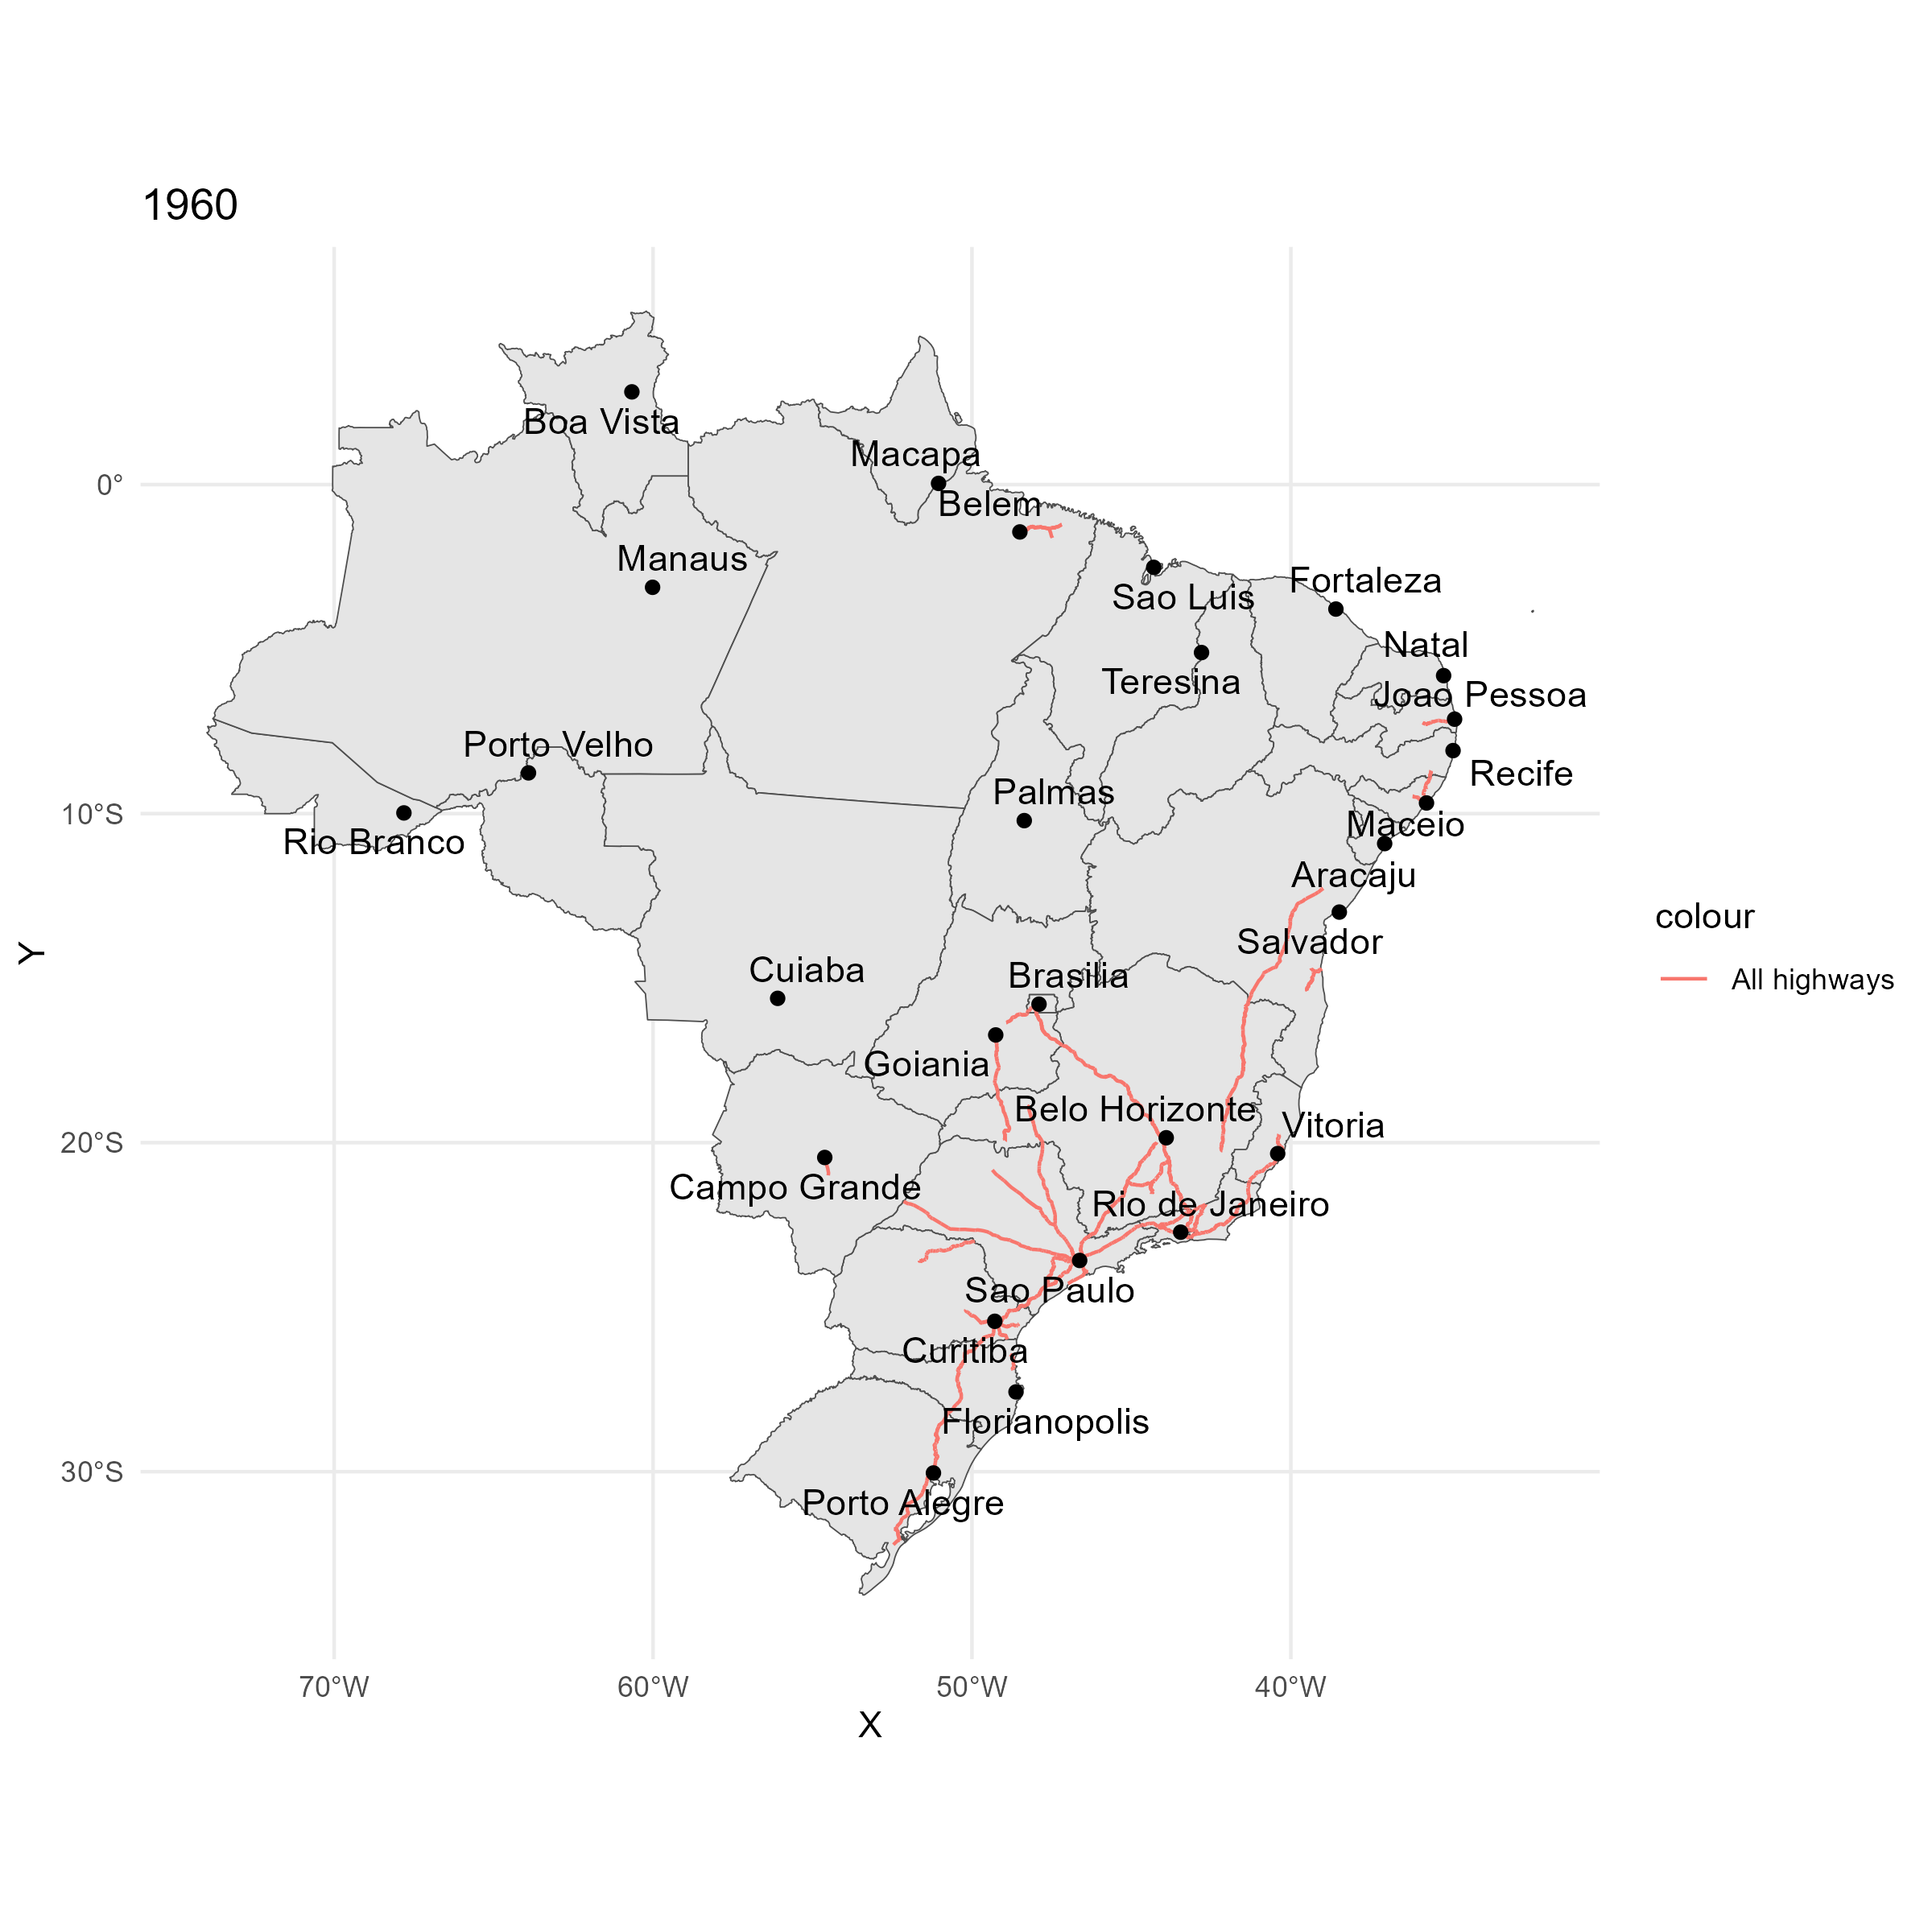
\includegraphics[width=\textwidth]{figures/appendix/roads/roads1960.png}    \end{subfigure}
    \hfill 
    \begin{subfigure}{0.32\textwidth}
        \centering
        \caption{1970}
        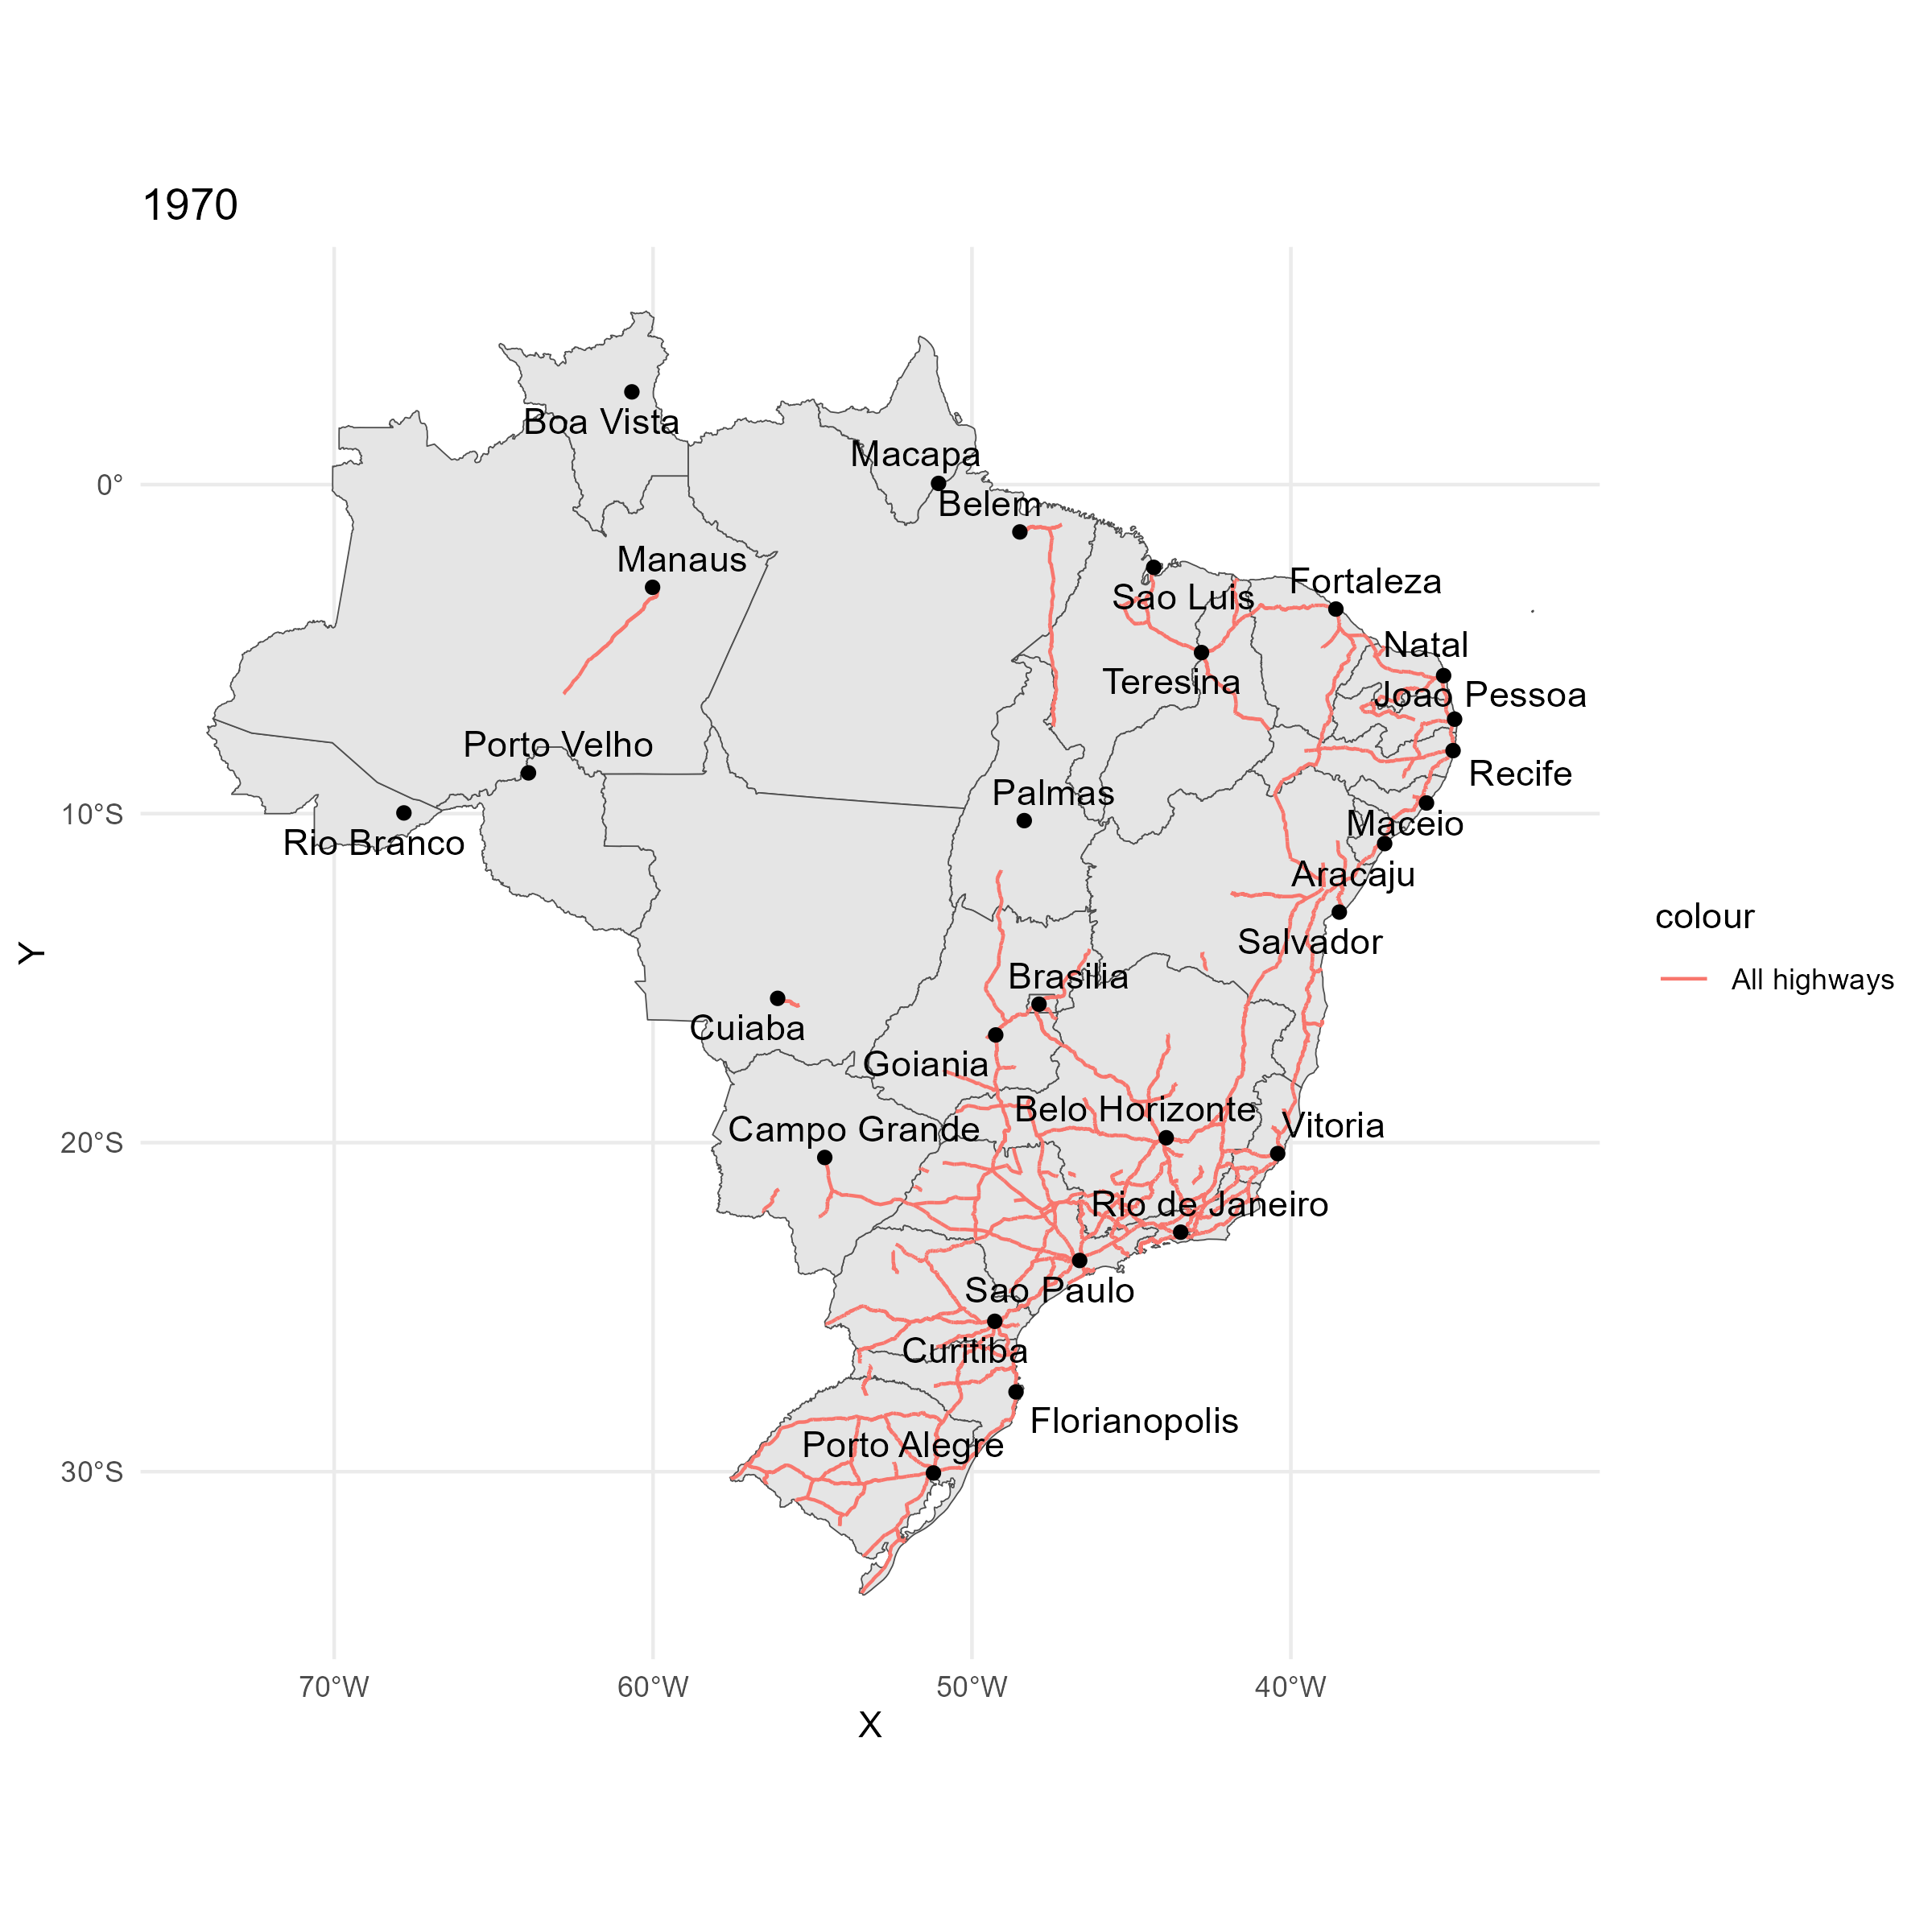
\includegraphics[width=\textwidth]{figures/appendix/roads/roads1970.png}
    \end{subfigure}
    \begin{subfigure}{0.32\textwidth}
        \centering
        \caption{1980}
        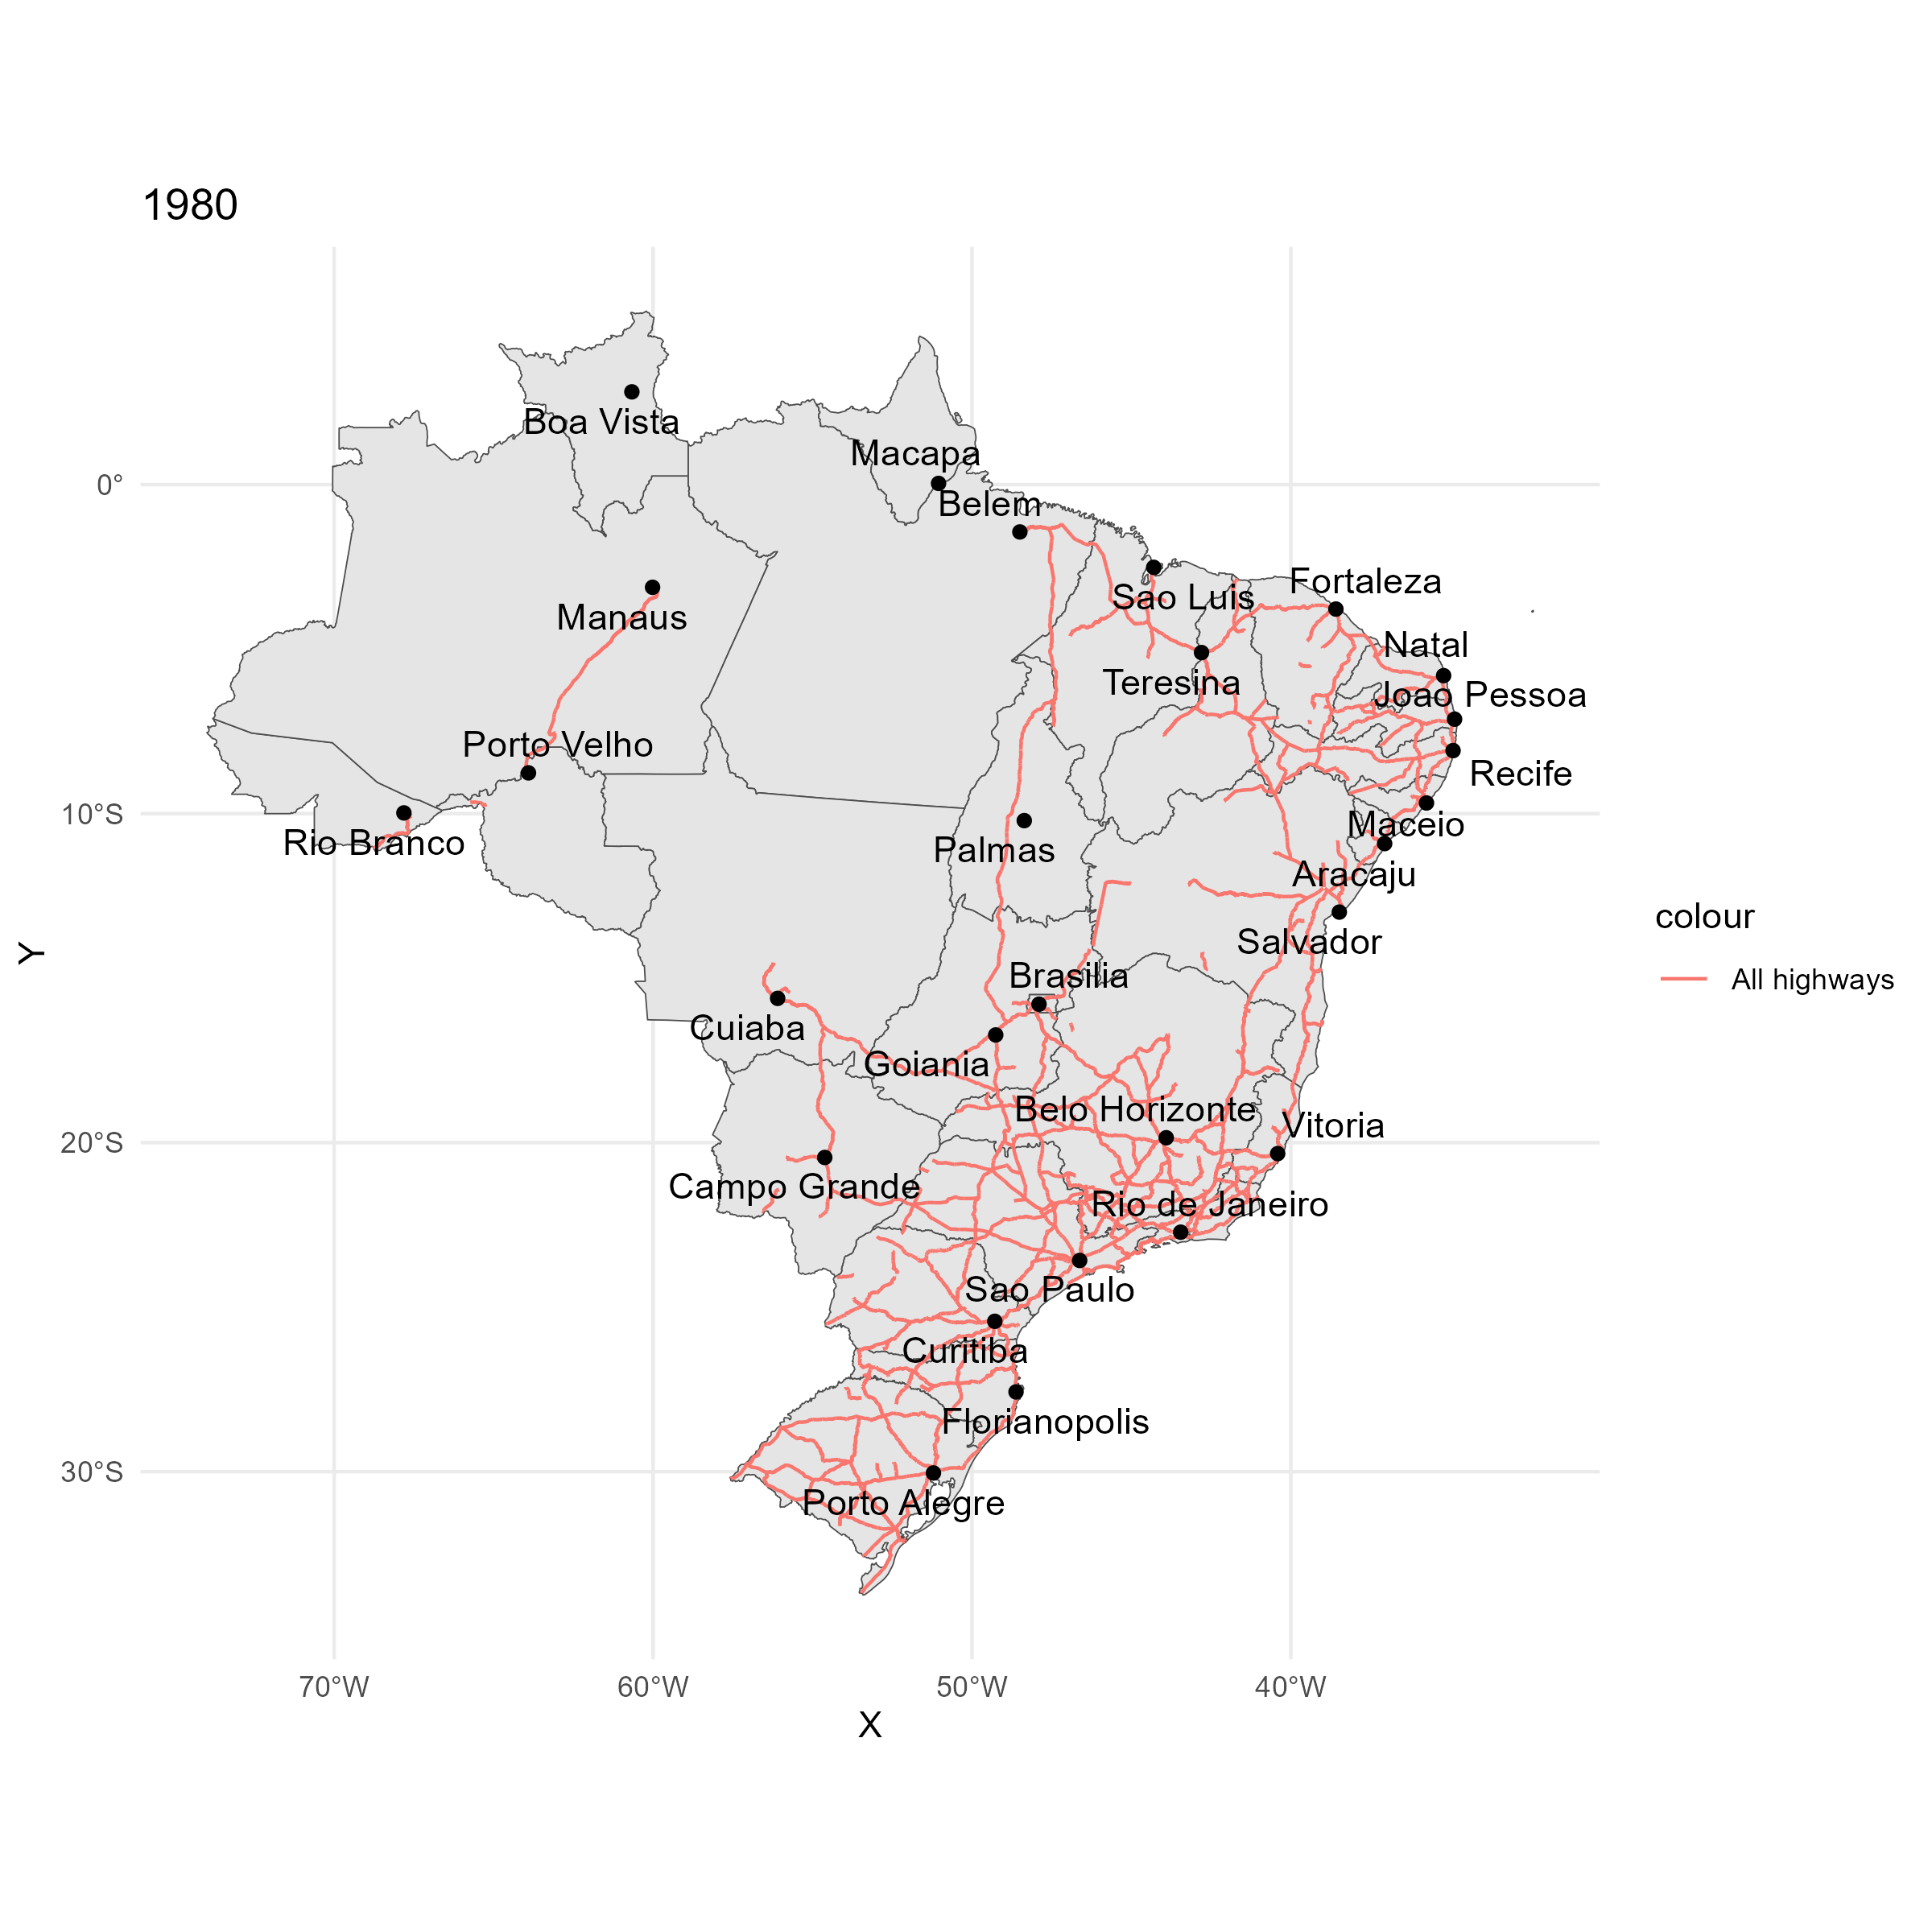
\includegraphics[width=\textwidth]{figures/appendix/roads/roads1980.png}
    \end{subfigure}
    \hfill
    \begin{subfigure}{0.32\textwidth}
        \centering
        \caption{1990}
        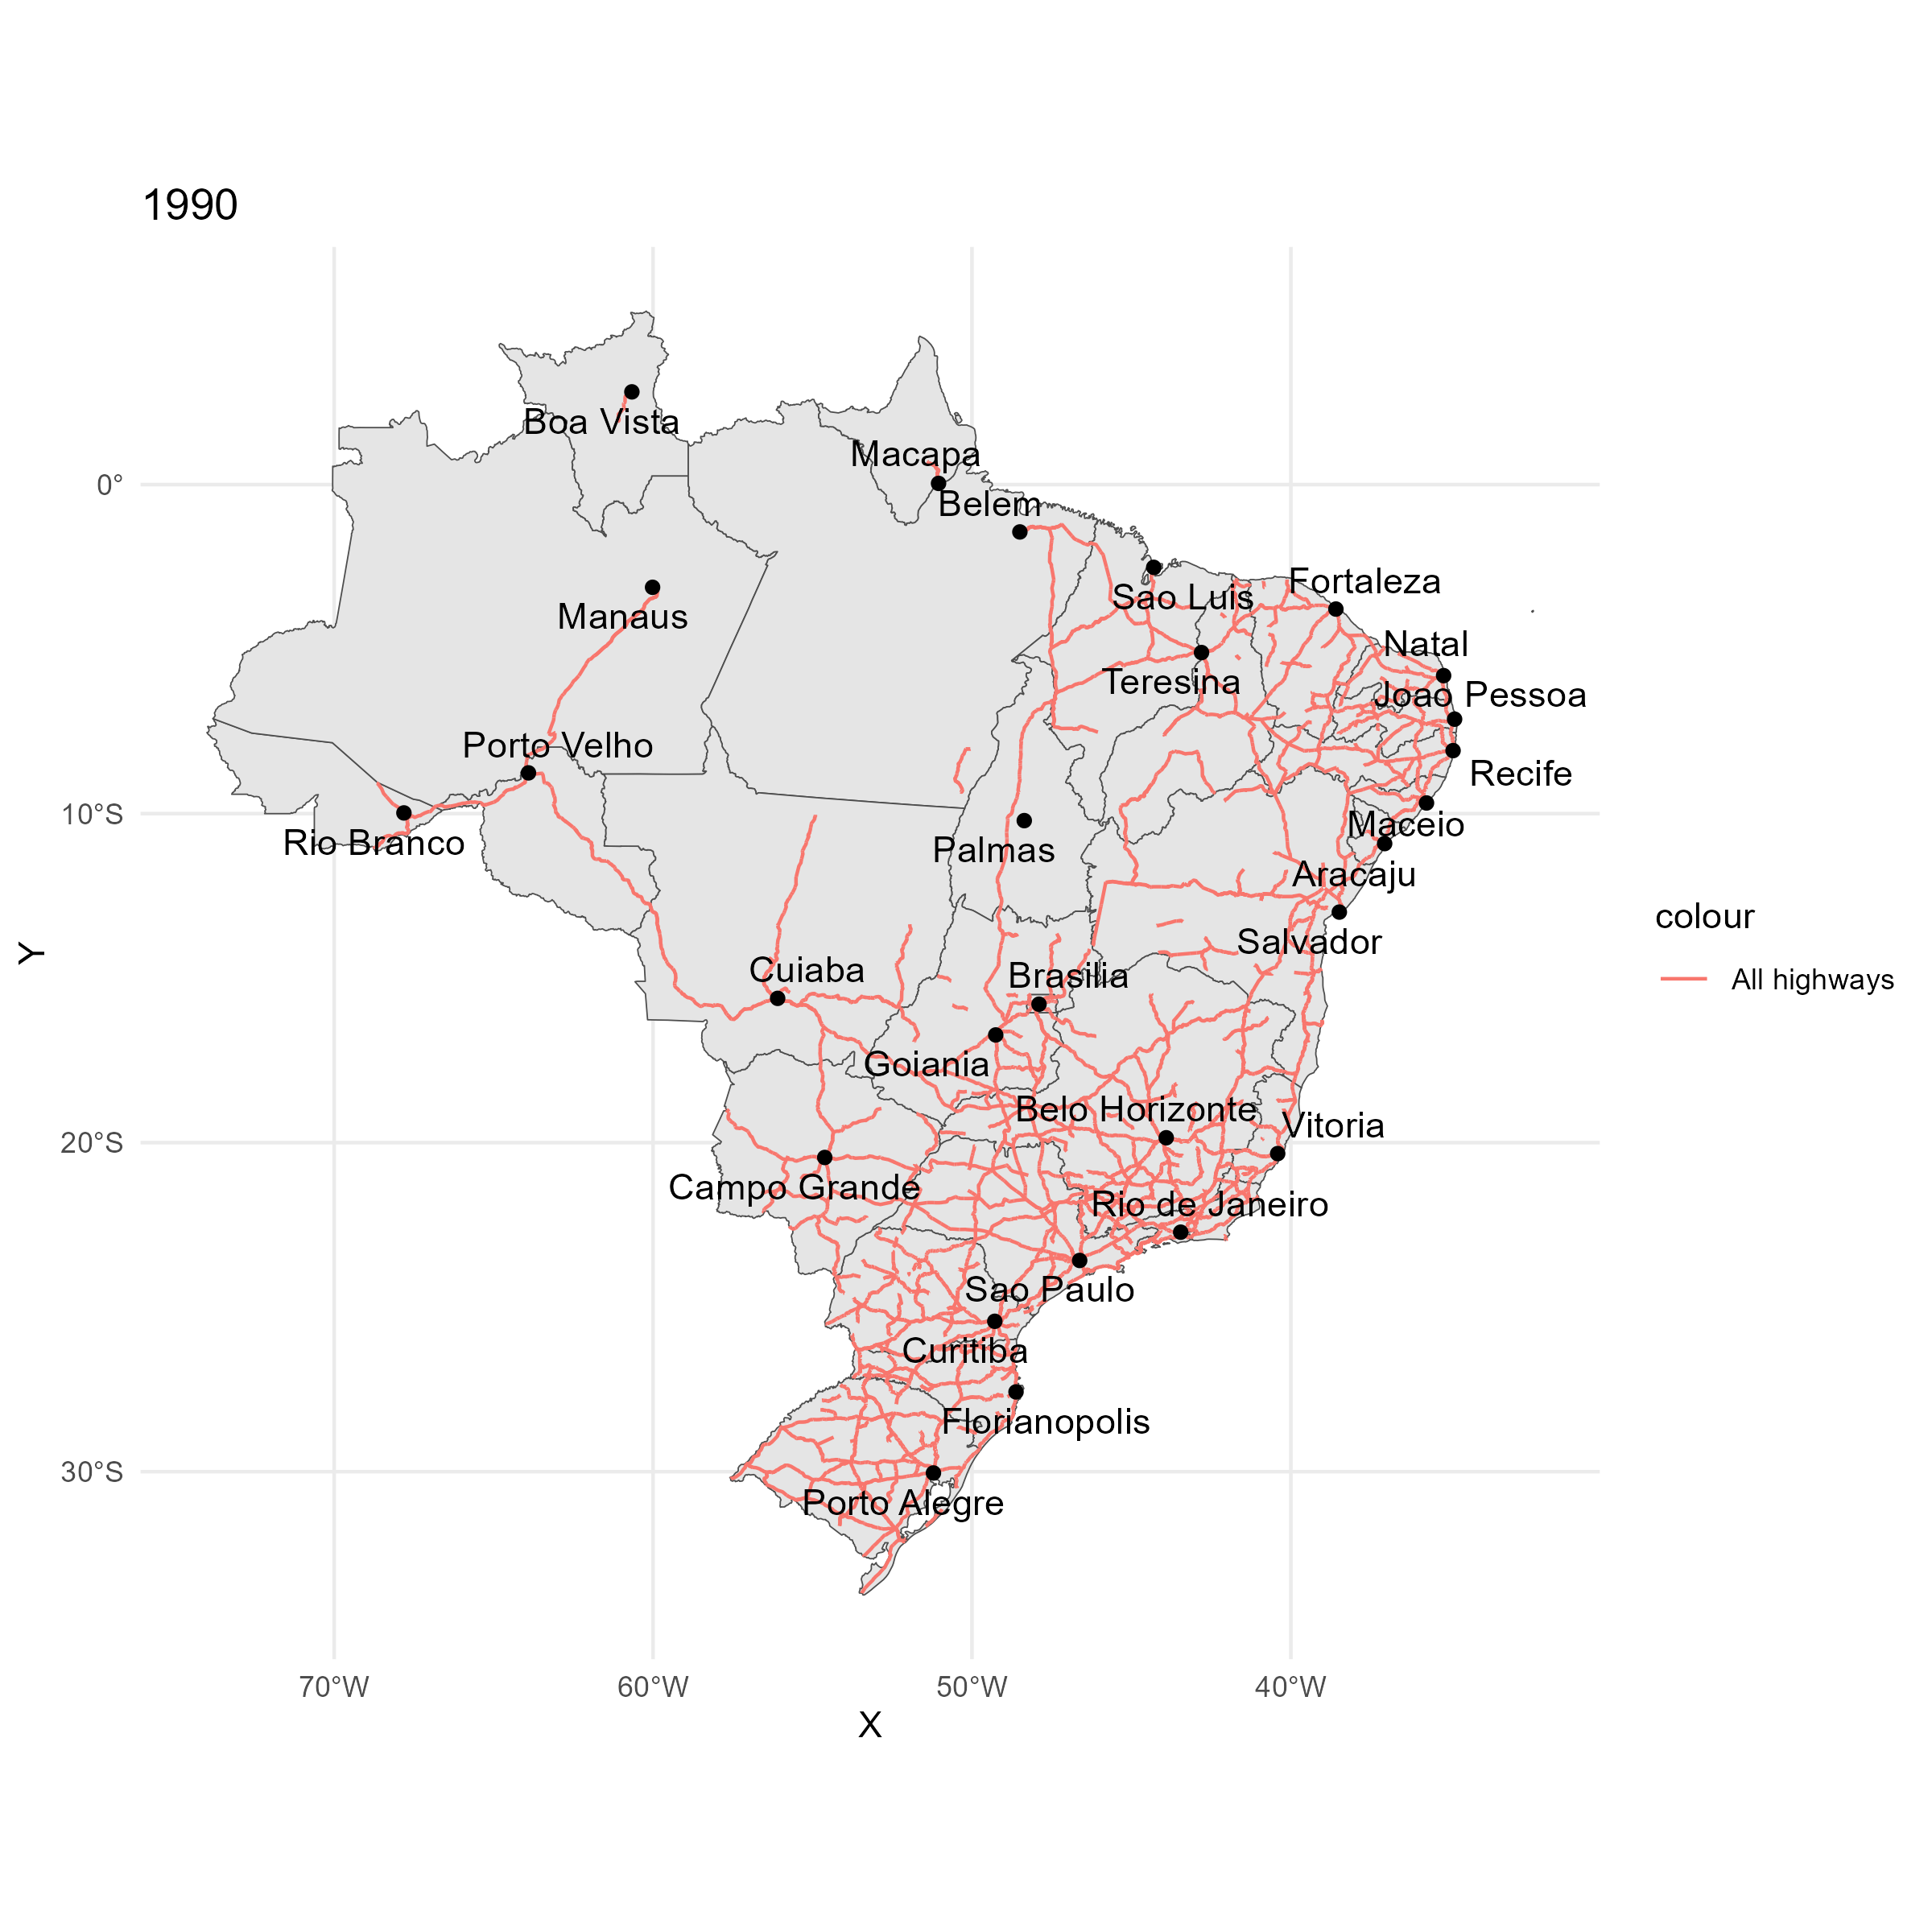
\includegraphics[width=\textwidth]{figures/appendix/roads/roads1990.png}
    \end{subfigure}
    \hfill
    \begin{subfigure}{0.32\textwidth}
        \centering
        \caption{2000}
        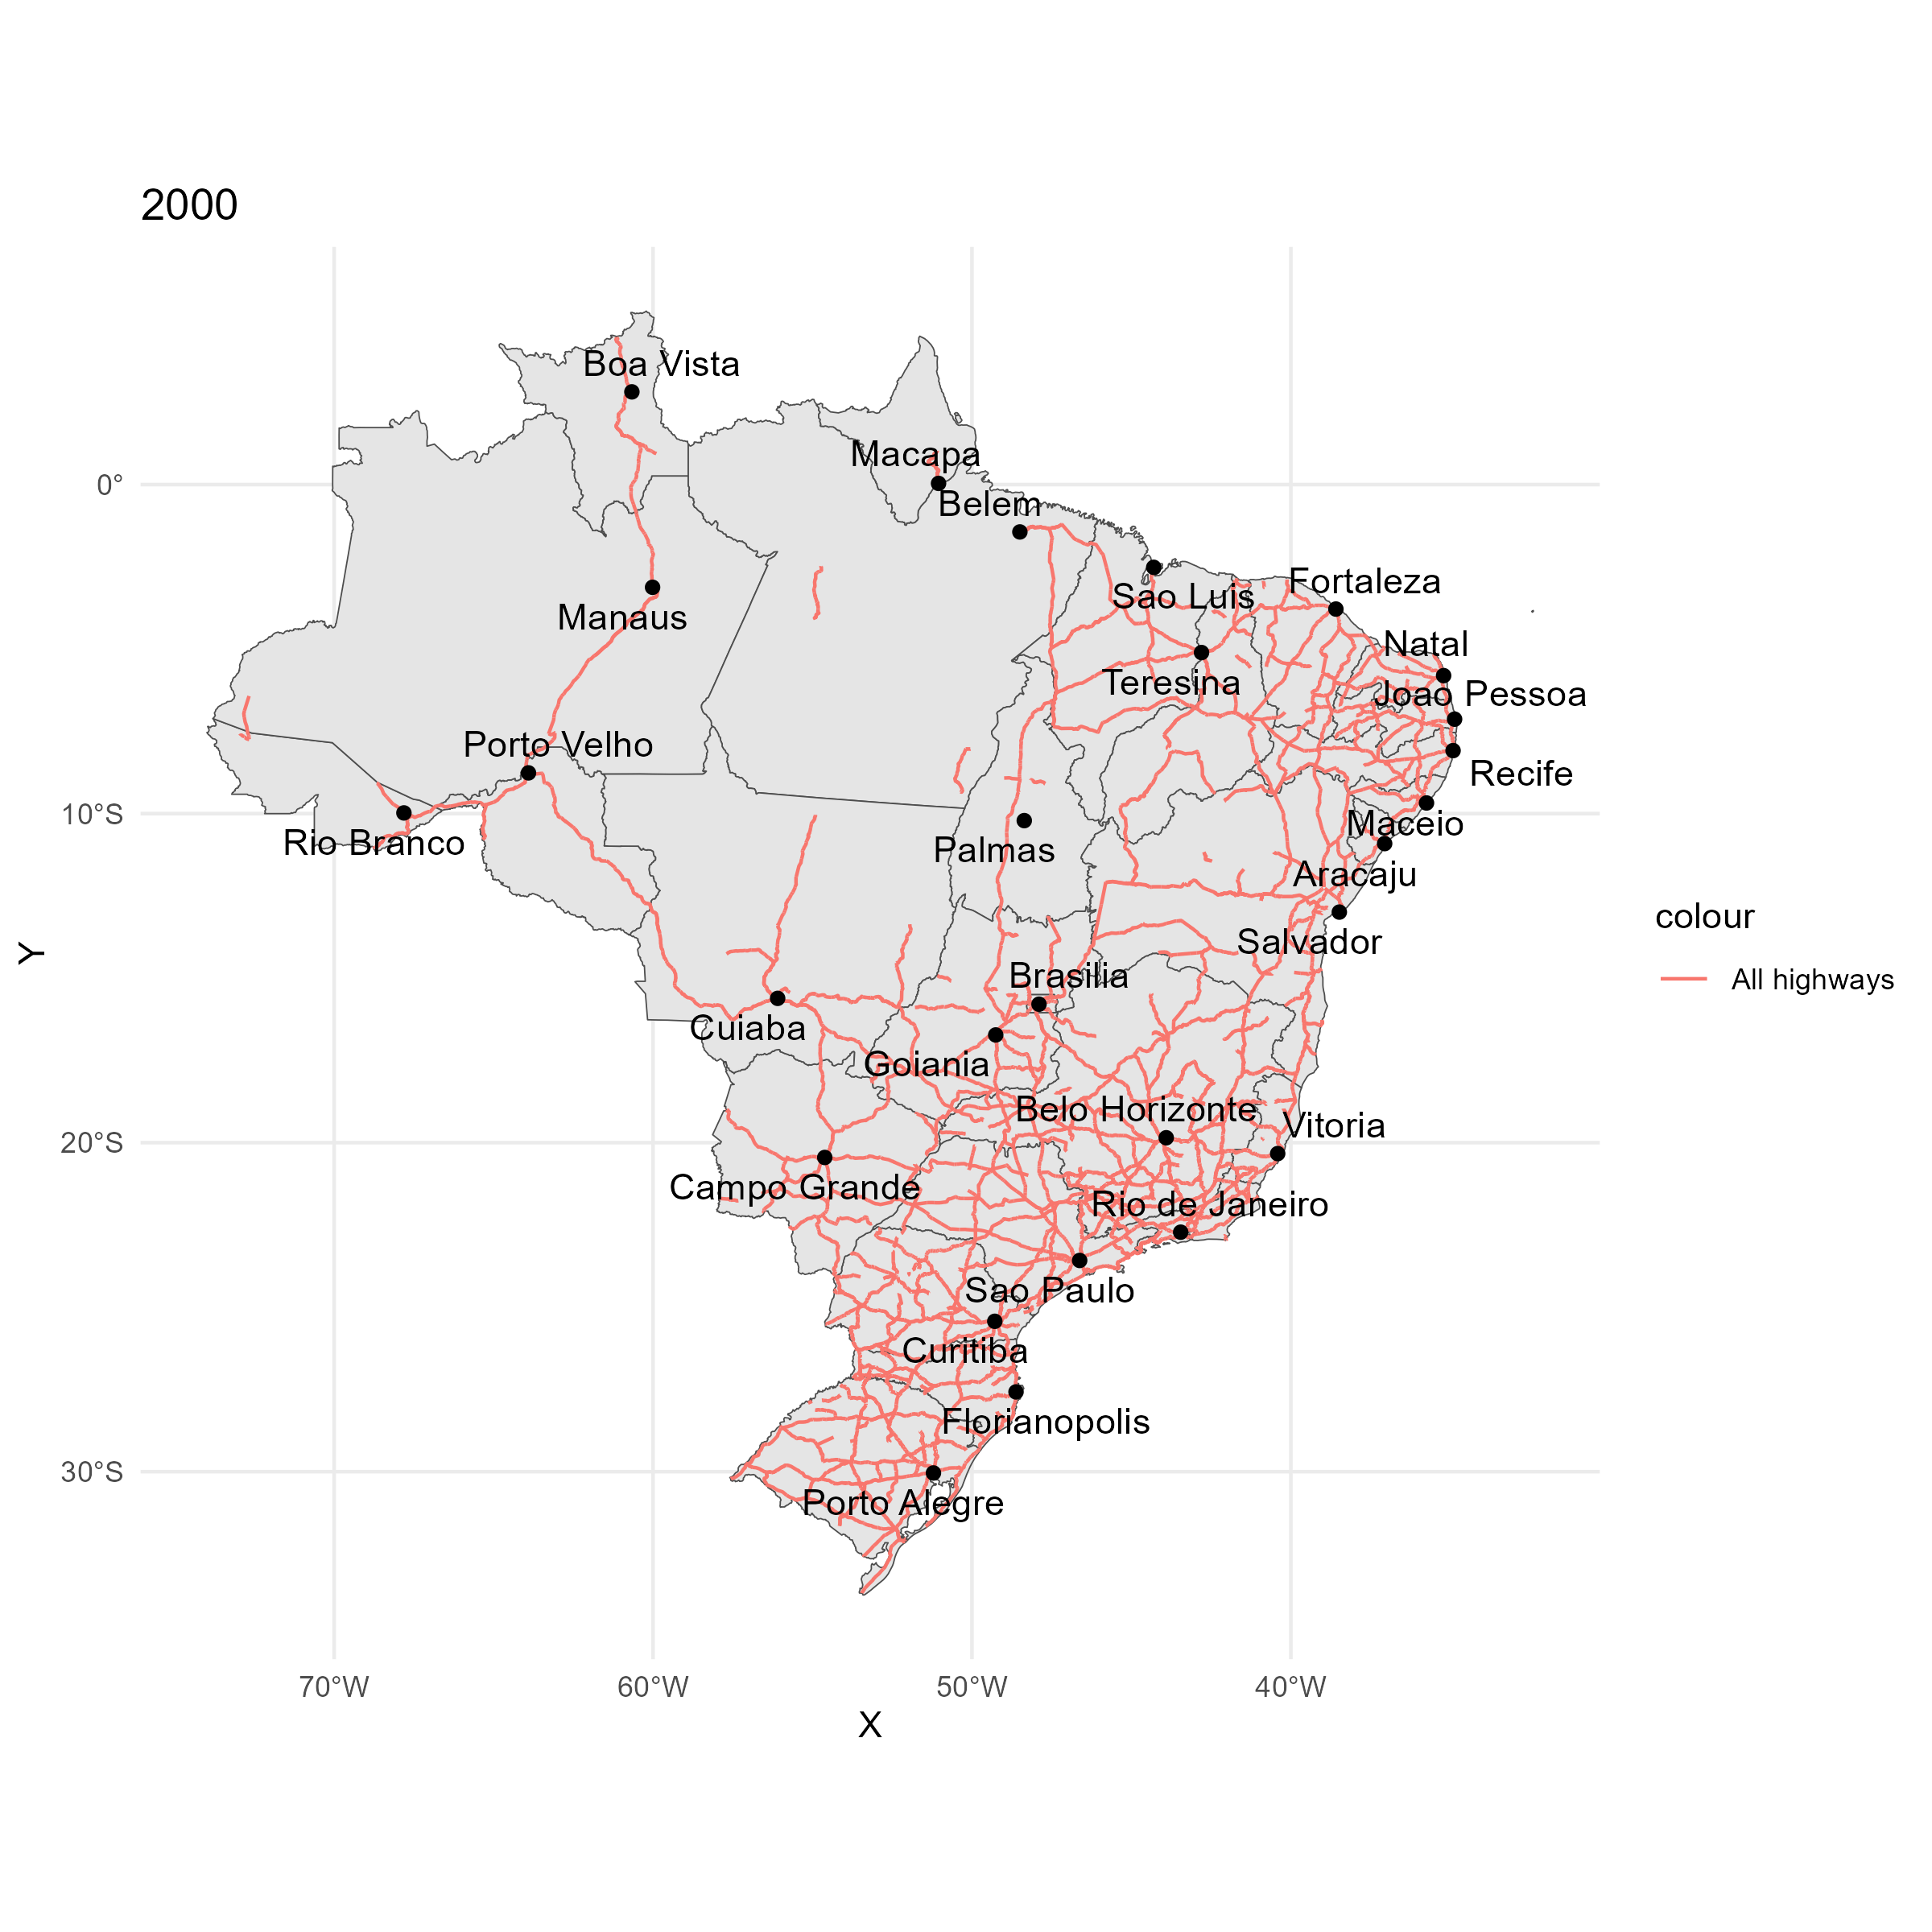
\includegraphics[width=\textwidth]{figures/appendix/roads/roads2000.png}
    \end{subfigure}
    \hfill
    \begin{subfigure}{0.32\textwidth}
        \centering
        \caption{2010}
        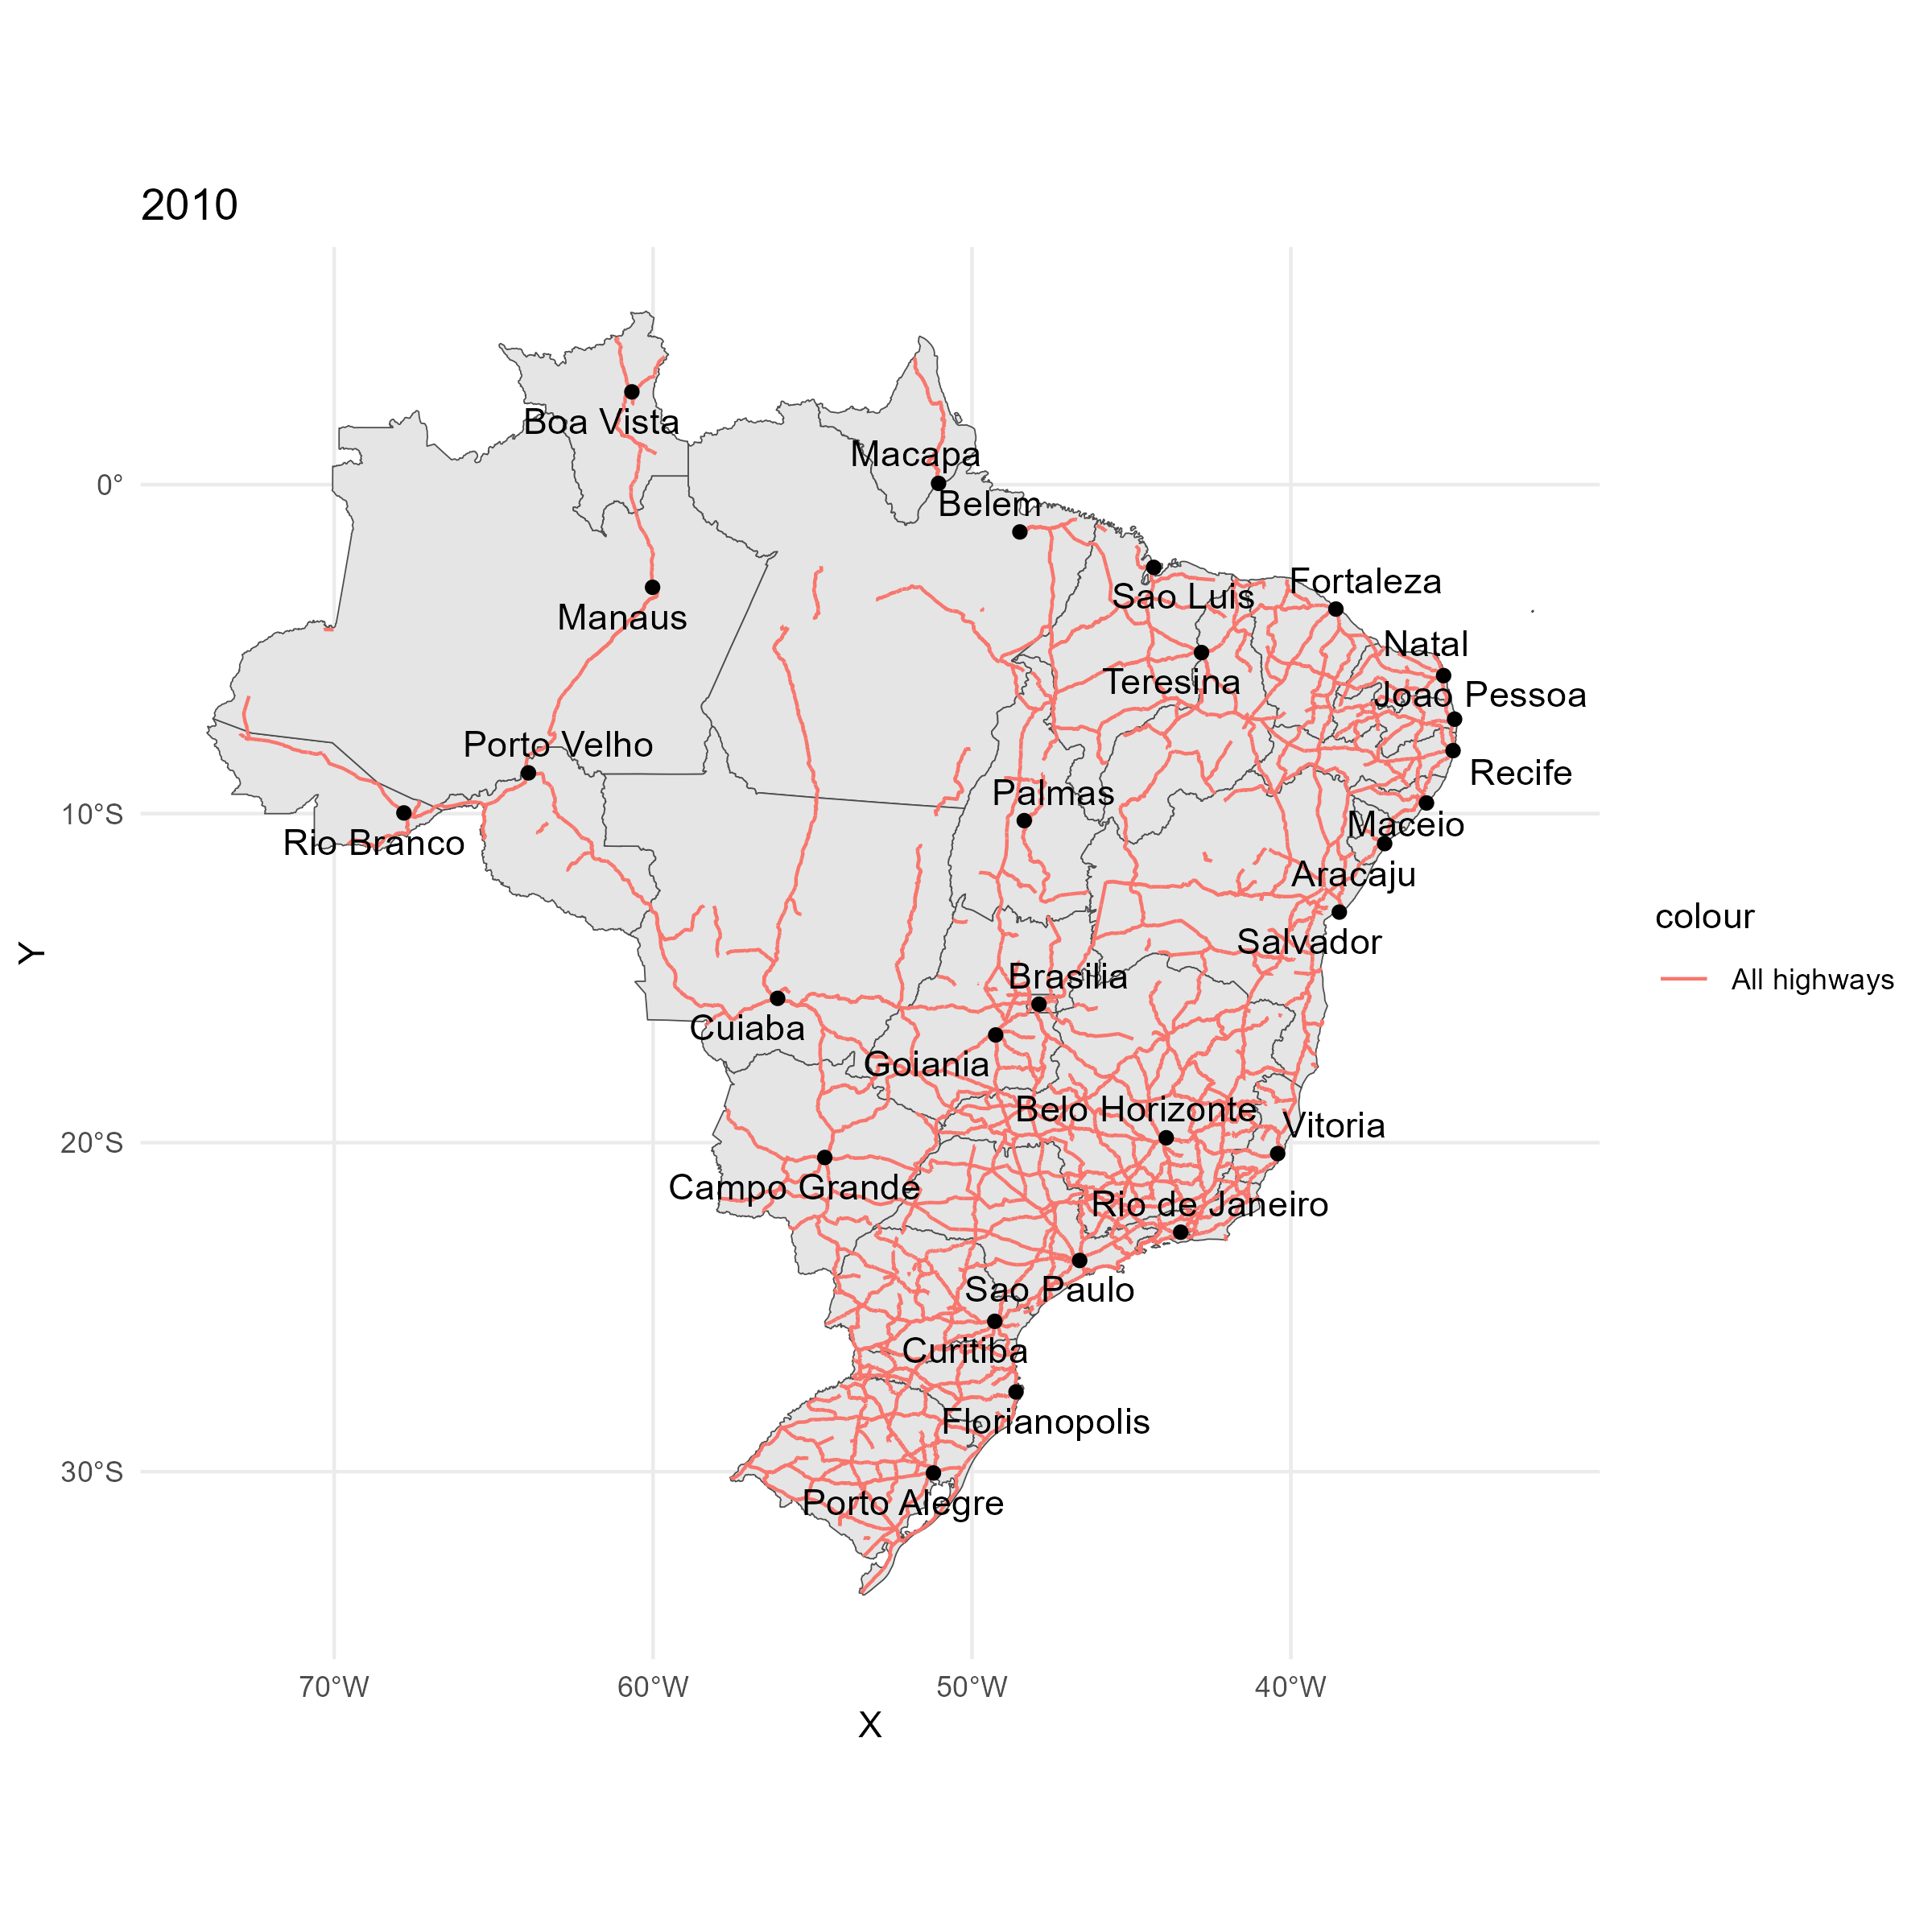
\includegraphics[width=\textwidth]{figures/appendix/roads/roads2010.png}
    \end{subfigure}
\end{figure}

\clearpage
\begin{figure}[H]
    \centering
    \caption*{Appendix Figure 2: Travel Time to the Closest Port - Fast Marching Method}
    \begin{subfigure}{0.32\textwidth}
        \centering
        \caption{1960}
        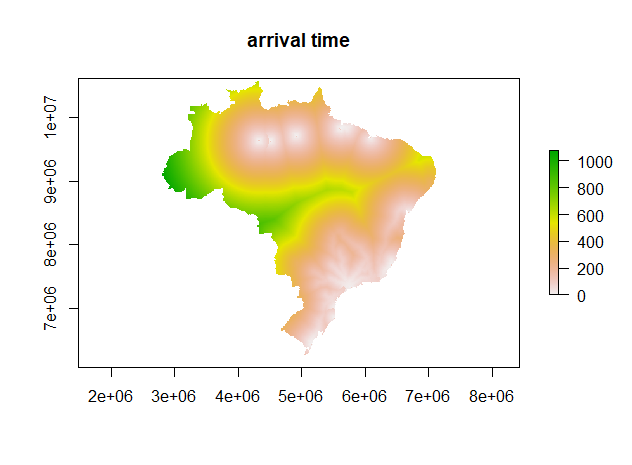
\includegraphics[width=\textwidth]{figures/appendix/fmm/highway_1960.png}    \end{subfigure}
    \hfill 
    \begin{subfigure}{0.32\textwidth}
        \centering
        \caption{1970}
        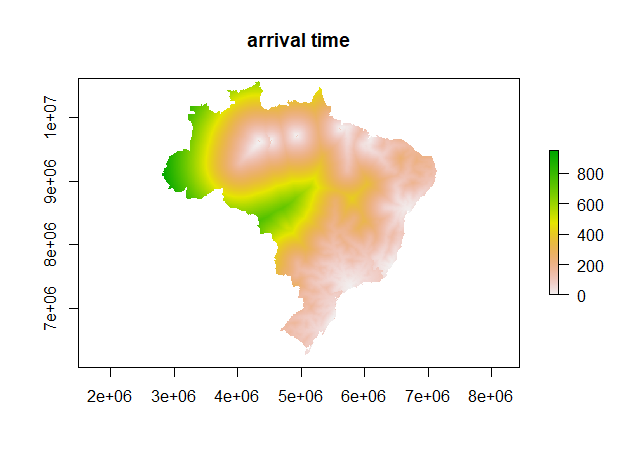
\includegraphics[width=\textwidth]{figures/appendix/fmm/fmm_1970.png}
    \end{subfigure}
    \begin{subfigure}{0.32\textwidth}
        \centering
        \caption{1980}
        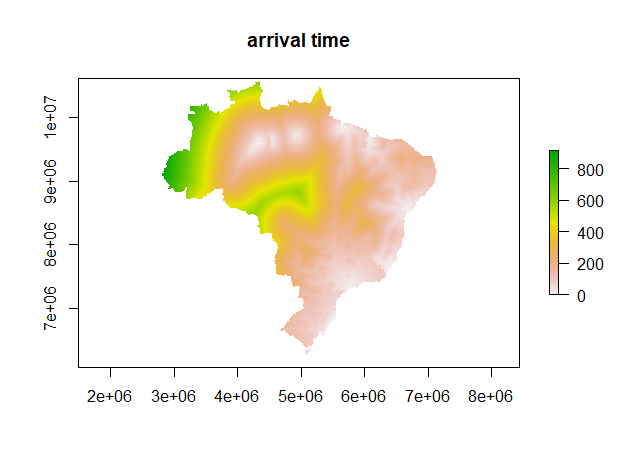
\includegraphics[width=\textwidth]{figures/appendix/fmm/highway_1980.png}
    \end{subfigure}
    \hfill
    \begin{subfigure}{0.32\textwidth}
        \centering
        \caption{1990}
        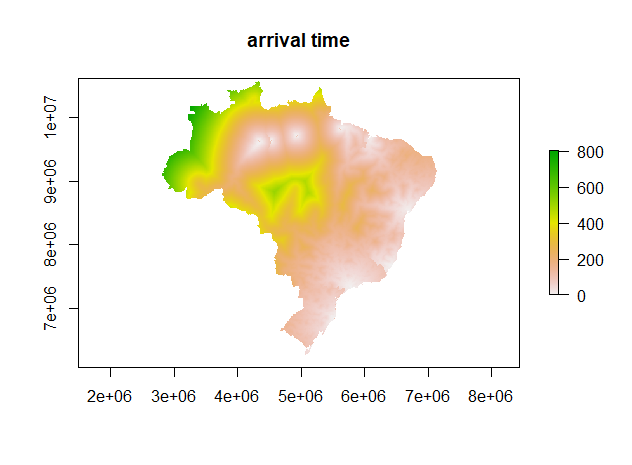
\includegraphics[width=\textwidth]{figures/appendix/fmm/highway_1990.png}
    \end{subfigure}
    \hfill
    \begin{subfigure}{0.32\textwidth}
        \centering
        \caption{2000}
        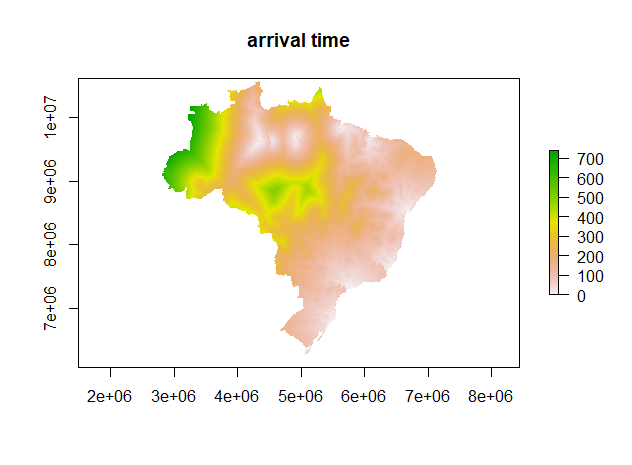
\includegraphics[width=\textwidth]{figures/appendix/fmm/highway_2000.png}
    \end{subfigure}
    \hfill
    \begin{subfigure}{0.32\textwidth}
        \centering
        \caption{2010}
        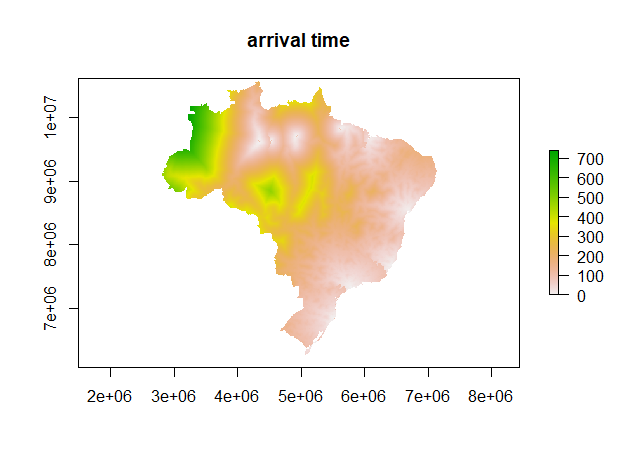
\includegraphics[width=\textwidth]{figures/appendix/fmm/highway_2010.png}
    \end{subfigure}
\end{figure}

\clearpage
\begin{figure}[H]
    \centering
    \caption*{Appendix Figure 3: Time-varying effects on Urban Population}
    
    \begin{subfigure}{0.50\textwidth}
        \centering
        \caption{TWFE}
        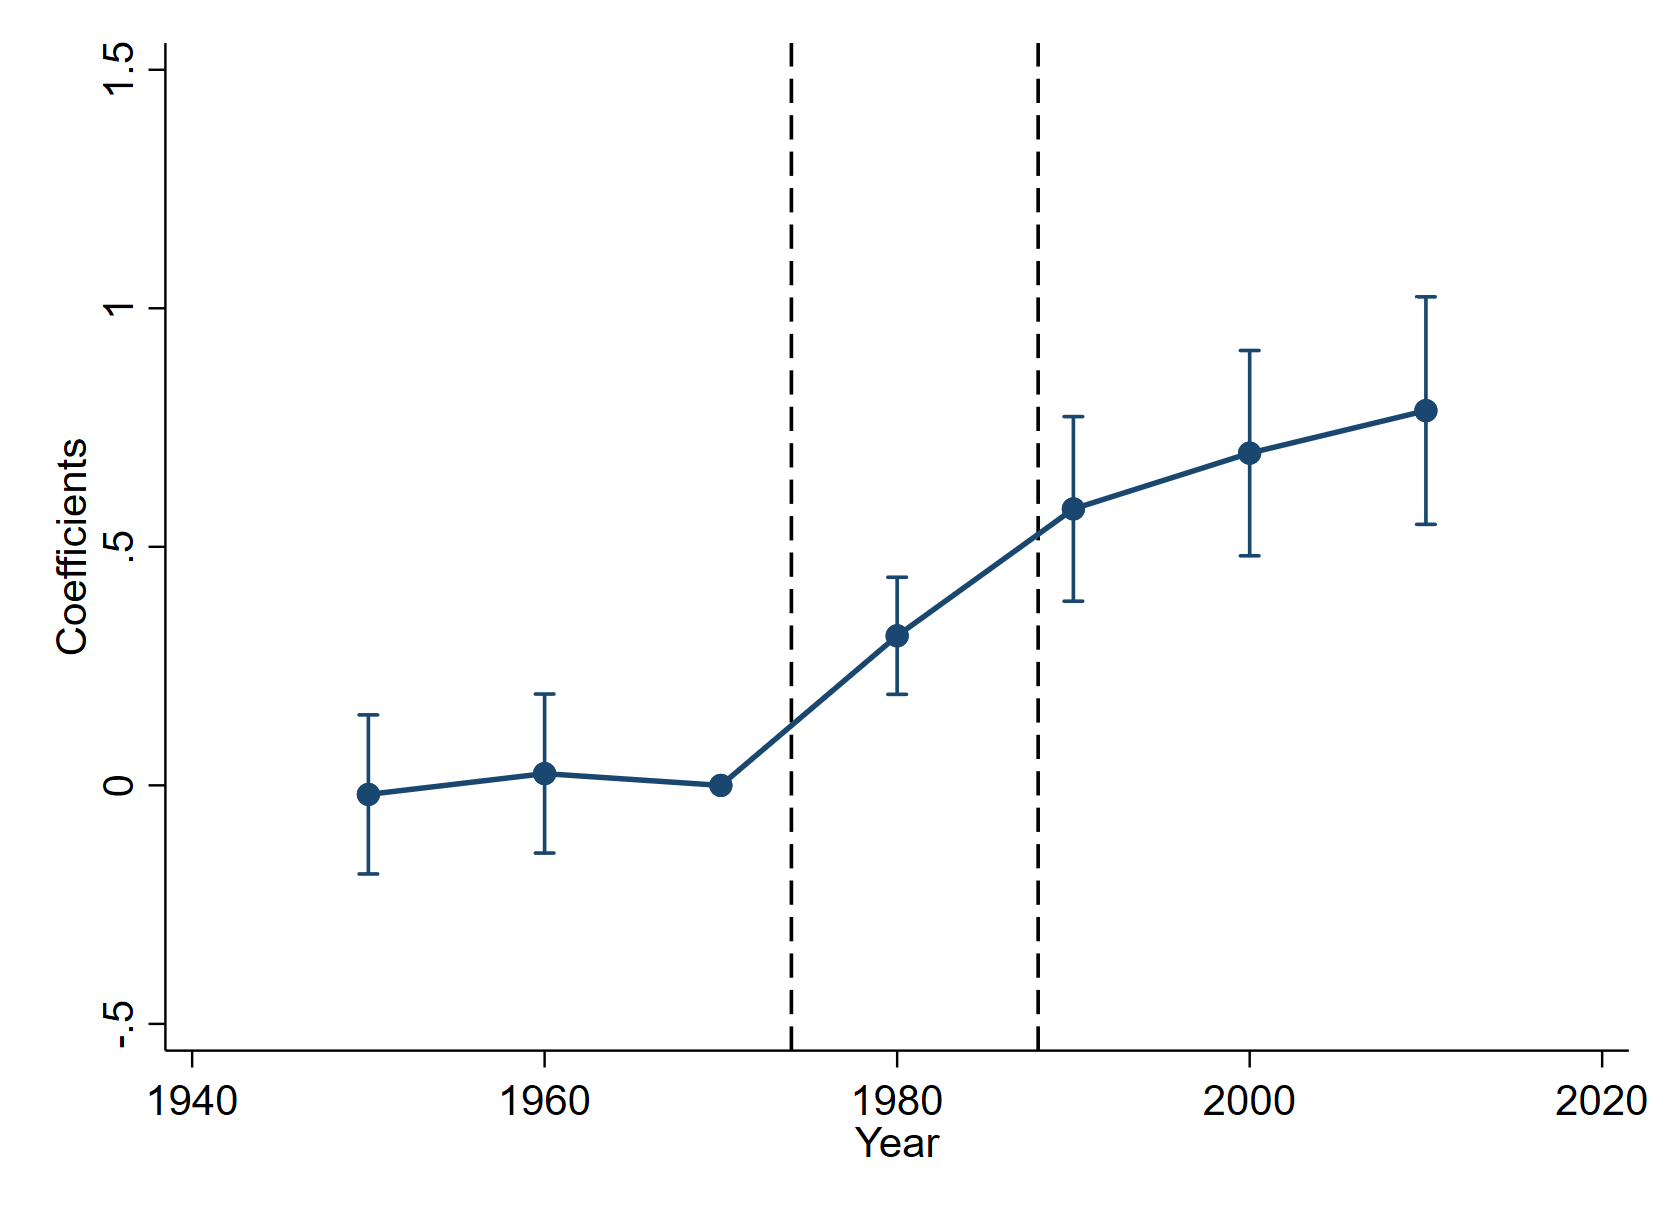
\includegraphics[width=\textwidth]{figures/urbpop.png}
    \end{subfigure}
    
    \begin{subfigure}{0.48\textwidth}
        \centering
        \caption{Borusyak et al (2022) Estimator}
        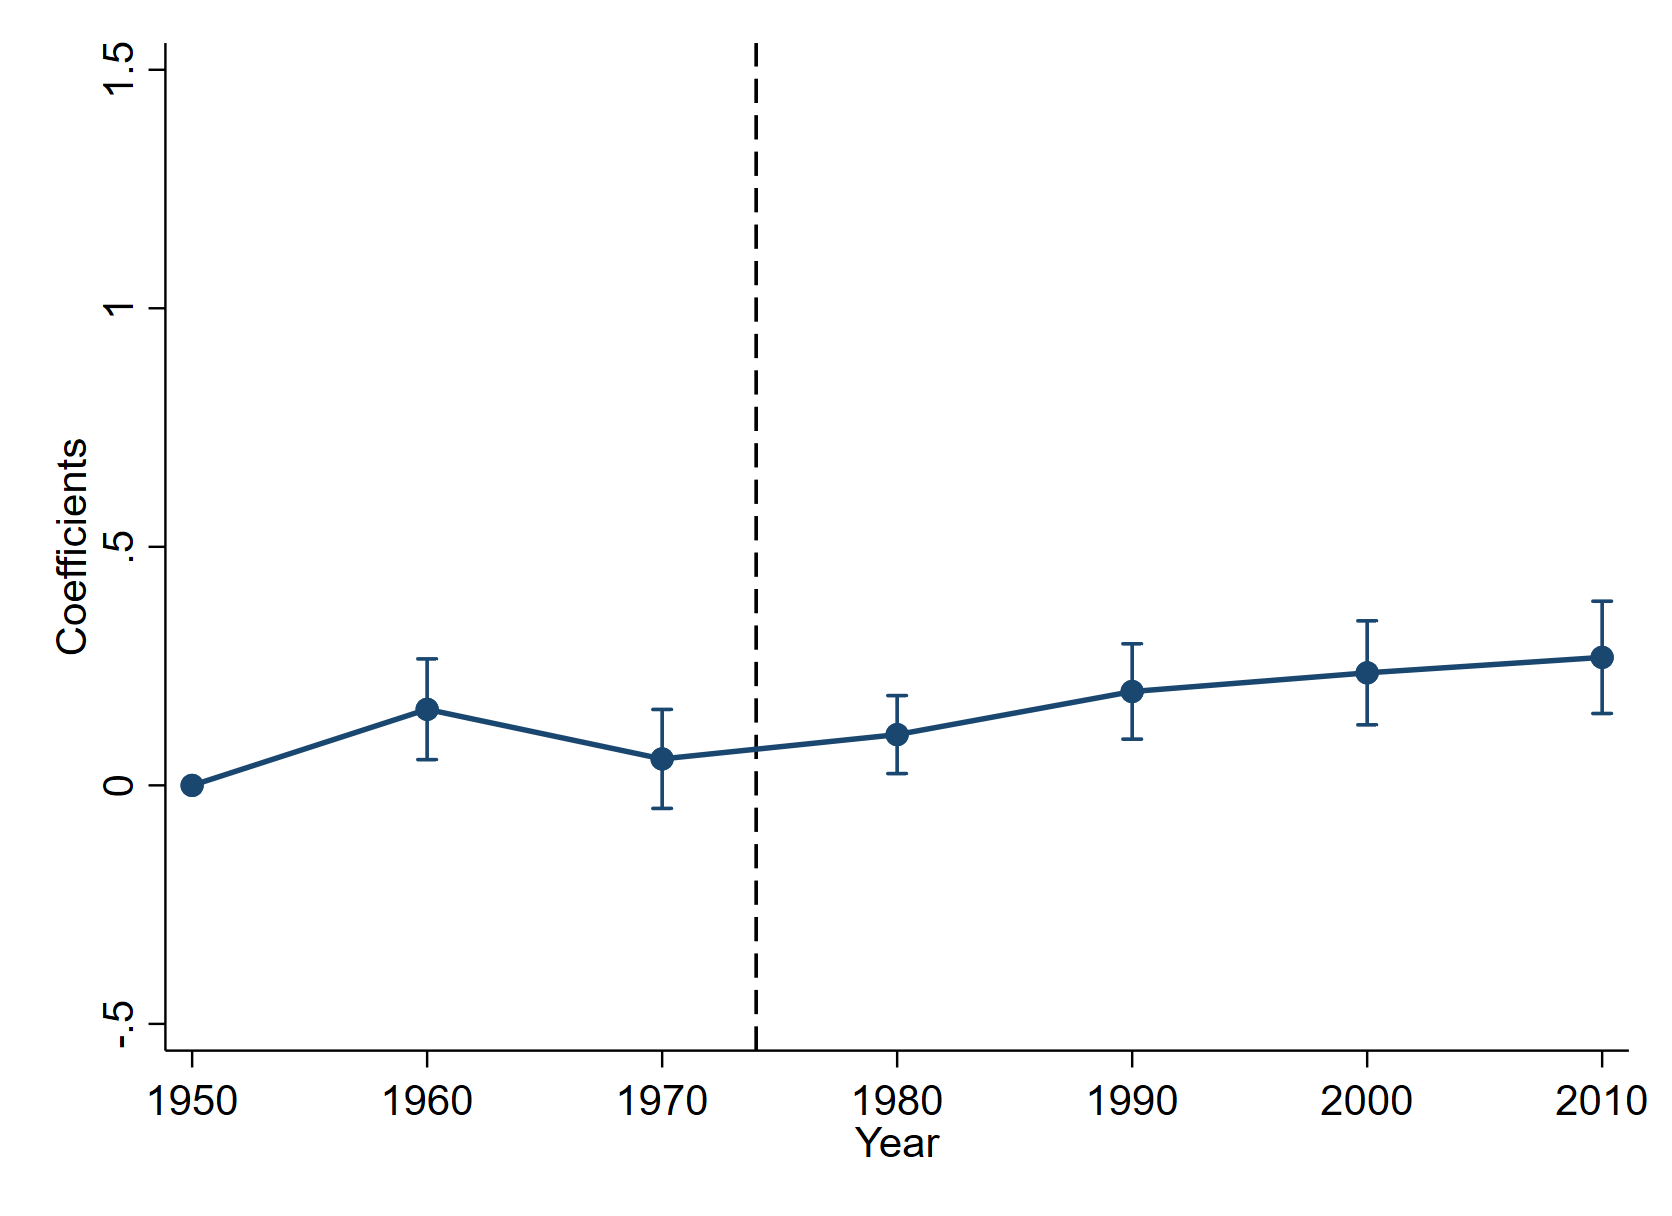
\includegraphics[width=\textwidth]{figures/appendix/urbpop_imputation.png}
    \end{subfigure}
    \begin{subfigure}{0.48\textwidth}
        \centering
        \caption{Callaway and Sant'Anna (2021) Estimator}
        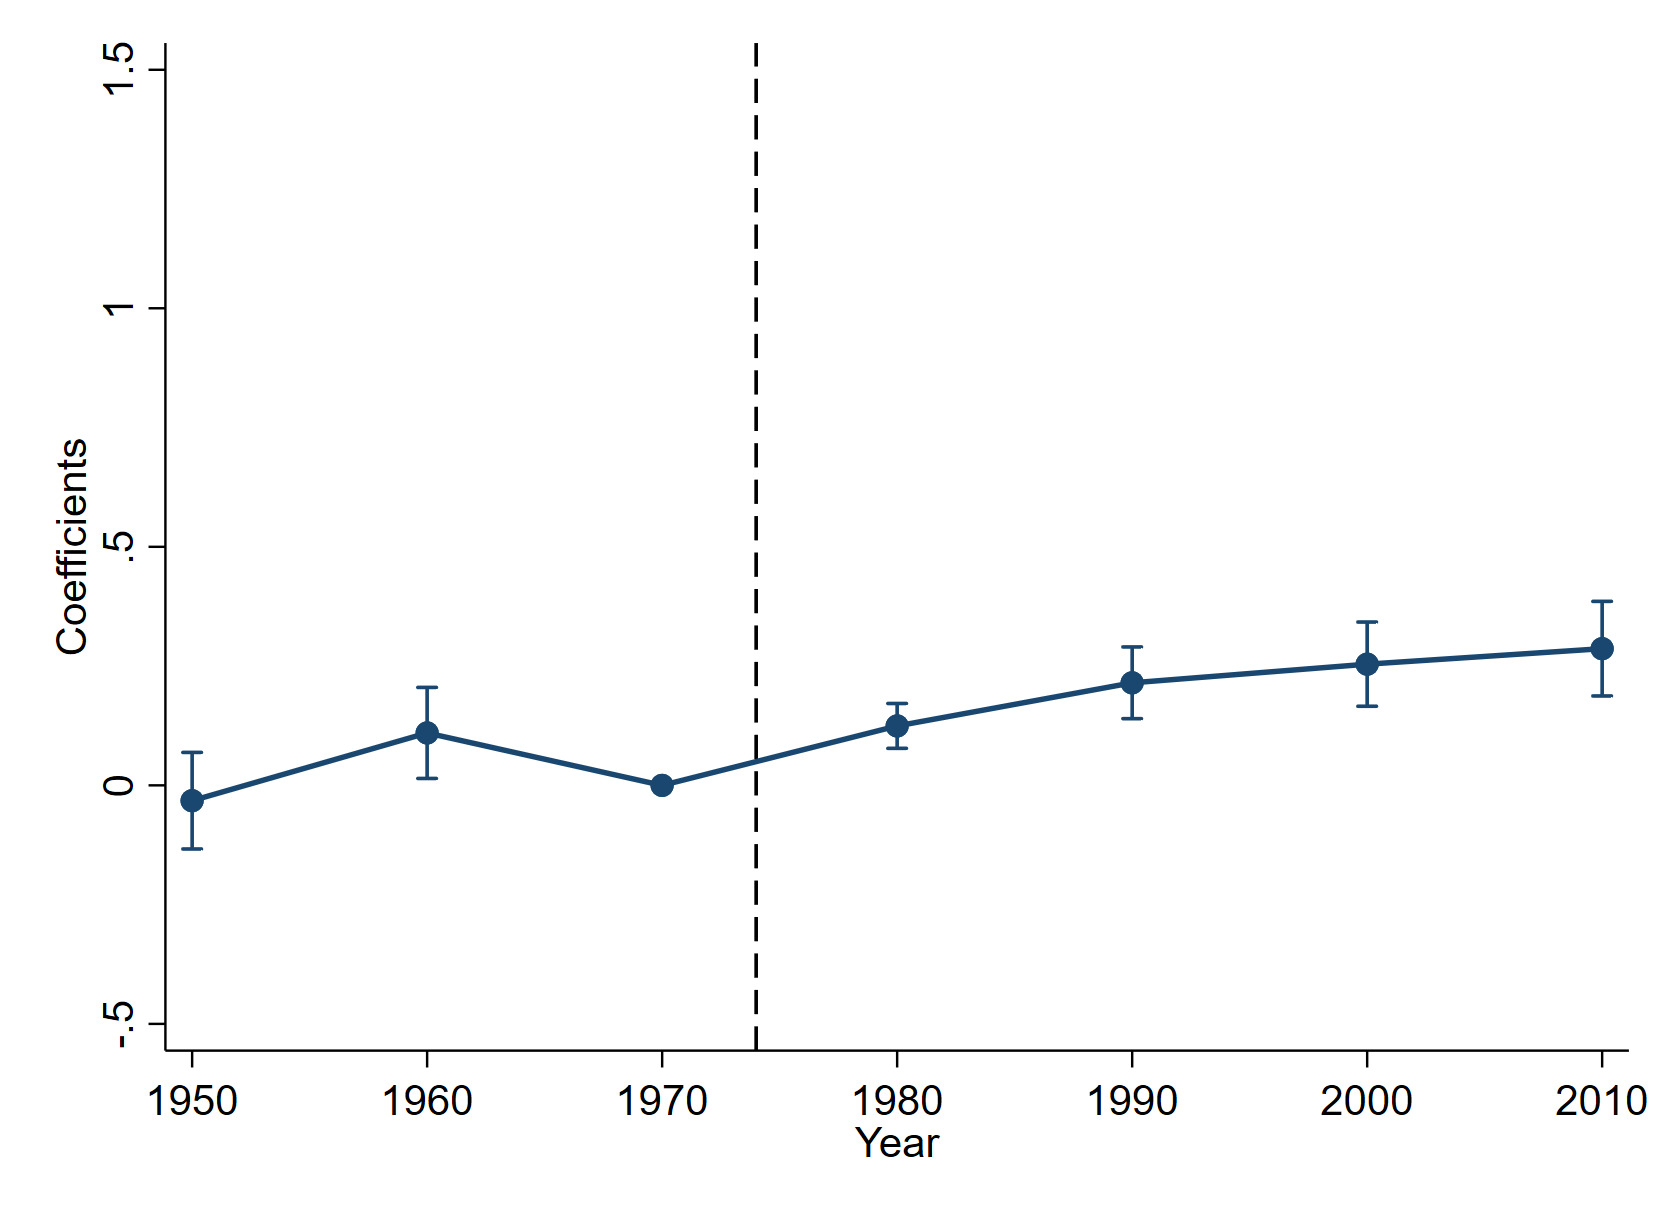
\includegraphics[width=\textwidth]{figures/appendix/urbpop_csdid.png}
    \end{subfigure}
\end{figure}

\clearpage
\begin{figure}[H]
    \centering
    \caption*{Appendix Figure 4: Time-varying effects on Urban Population Share}
    
    \begin{subfigure}{0.50\textwidth}
        \centering
        \caption{TWFE}
        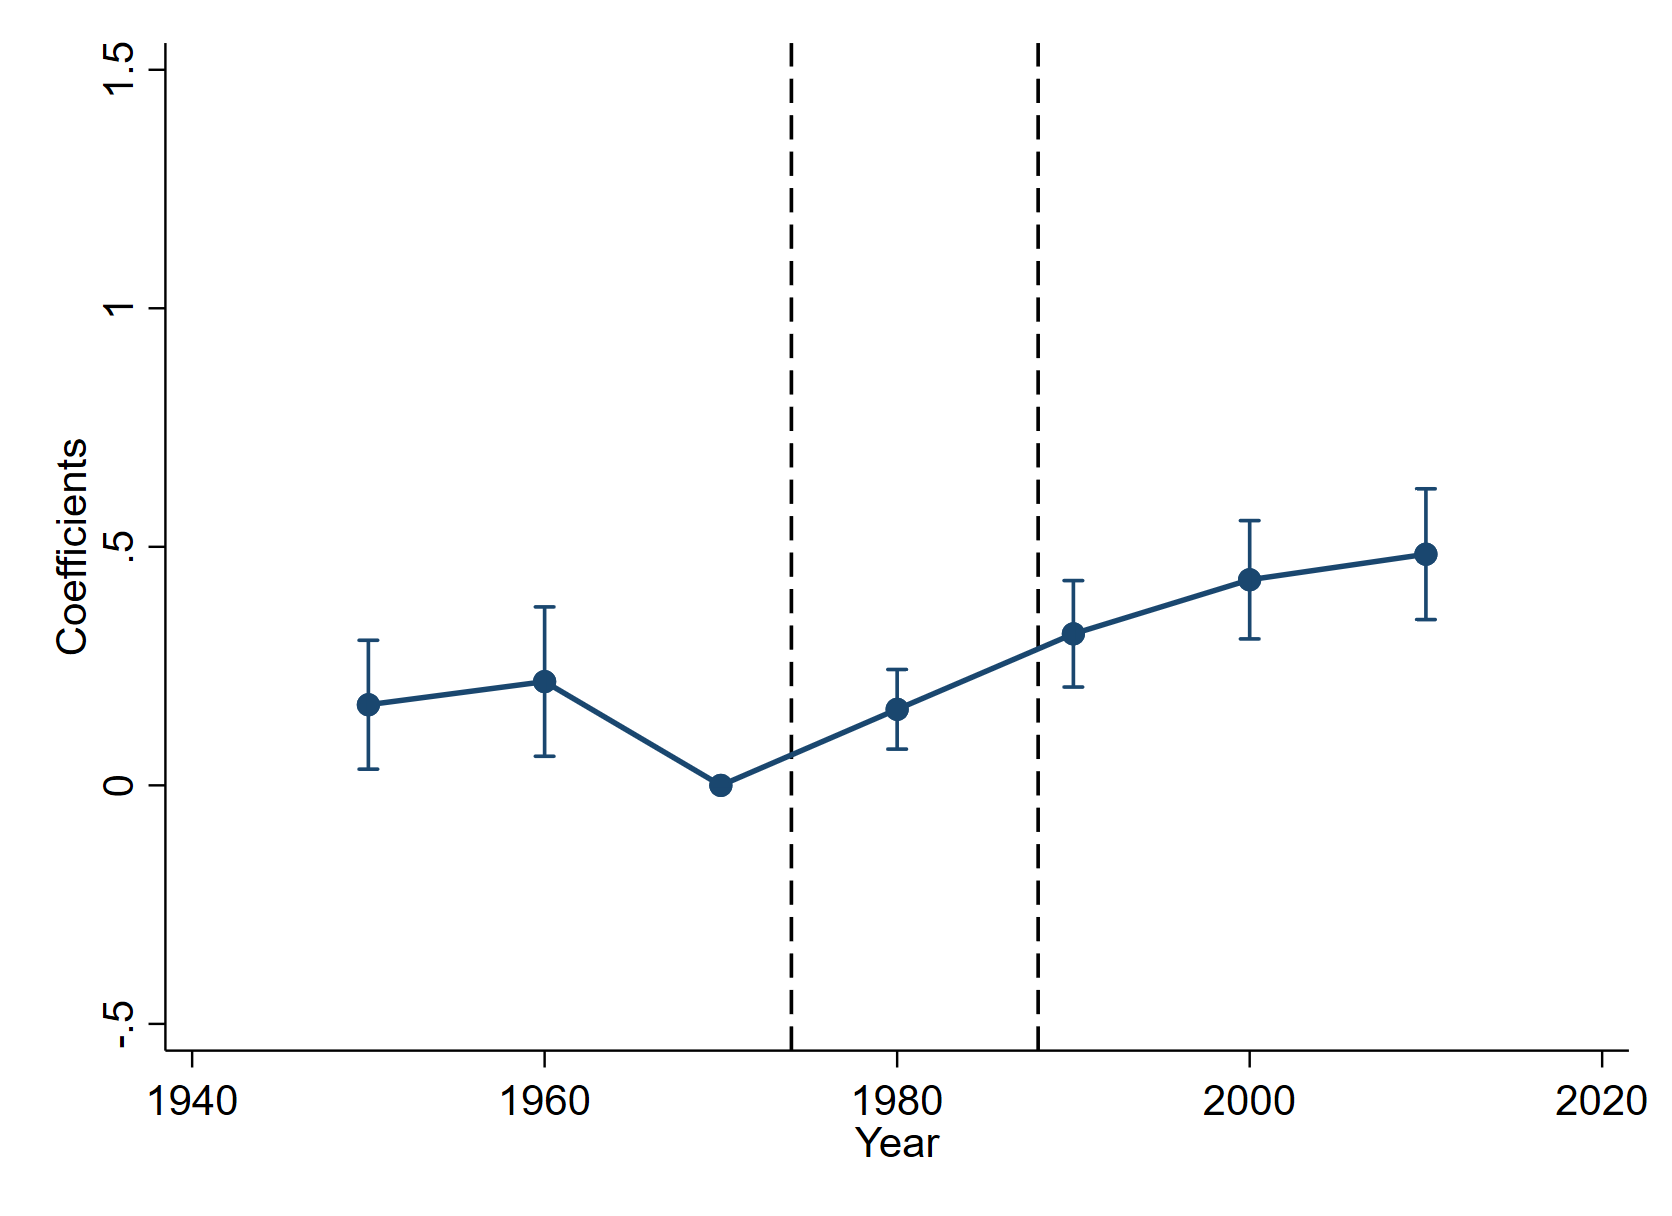
\includegraphics[width=\textwidth]{figures/urbshare.png}
    \end{subfigure}
    
    \begin{subfigure}{0.48\textwidth}
        \centering
        \caption{Borusyak et al (2022) Estimator}
        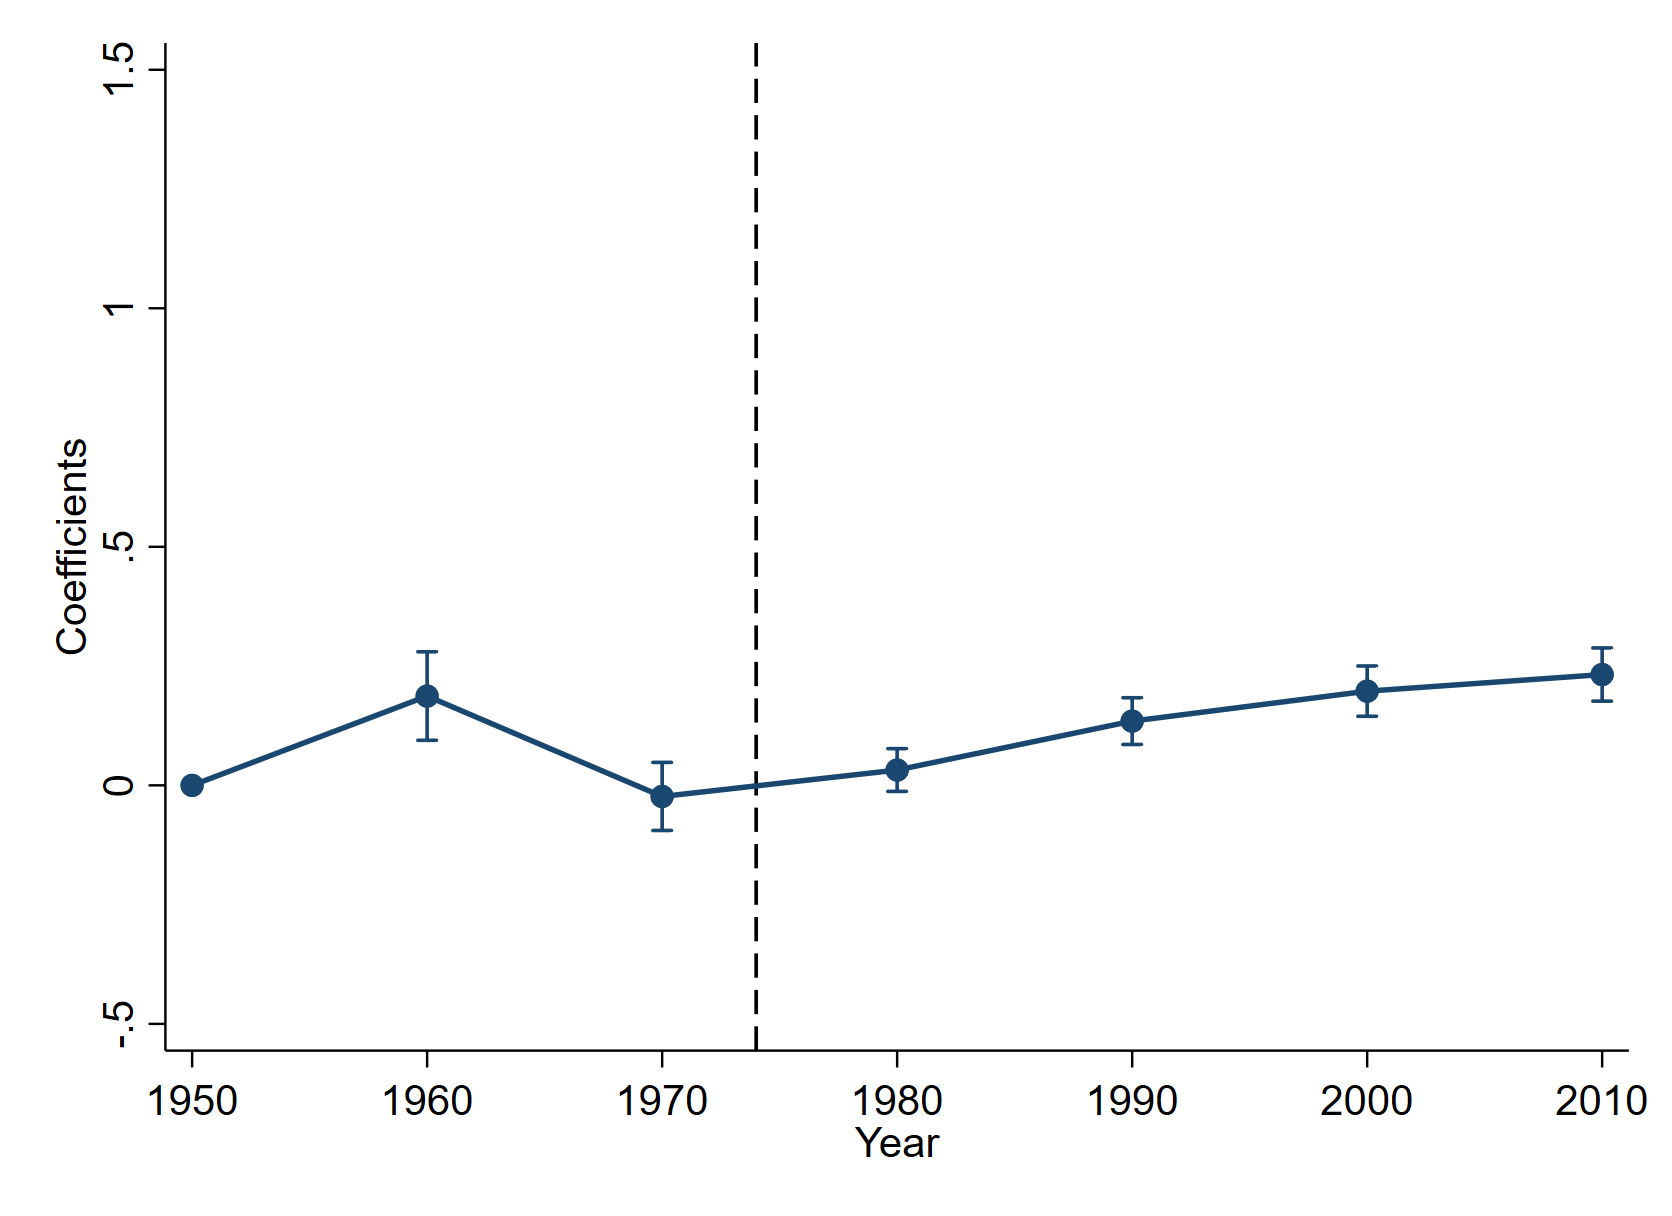
\includegraphics[width=\textwidth]{figures/appendix/urbshare_imputation.png}
    \end{subfigure}
    \begin{subfigure}{0.48\textwidth}
        \centering
        \caption{Callaway and Sant'Anna (2021) Estimator}
        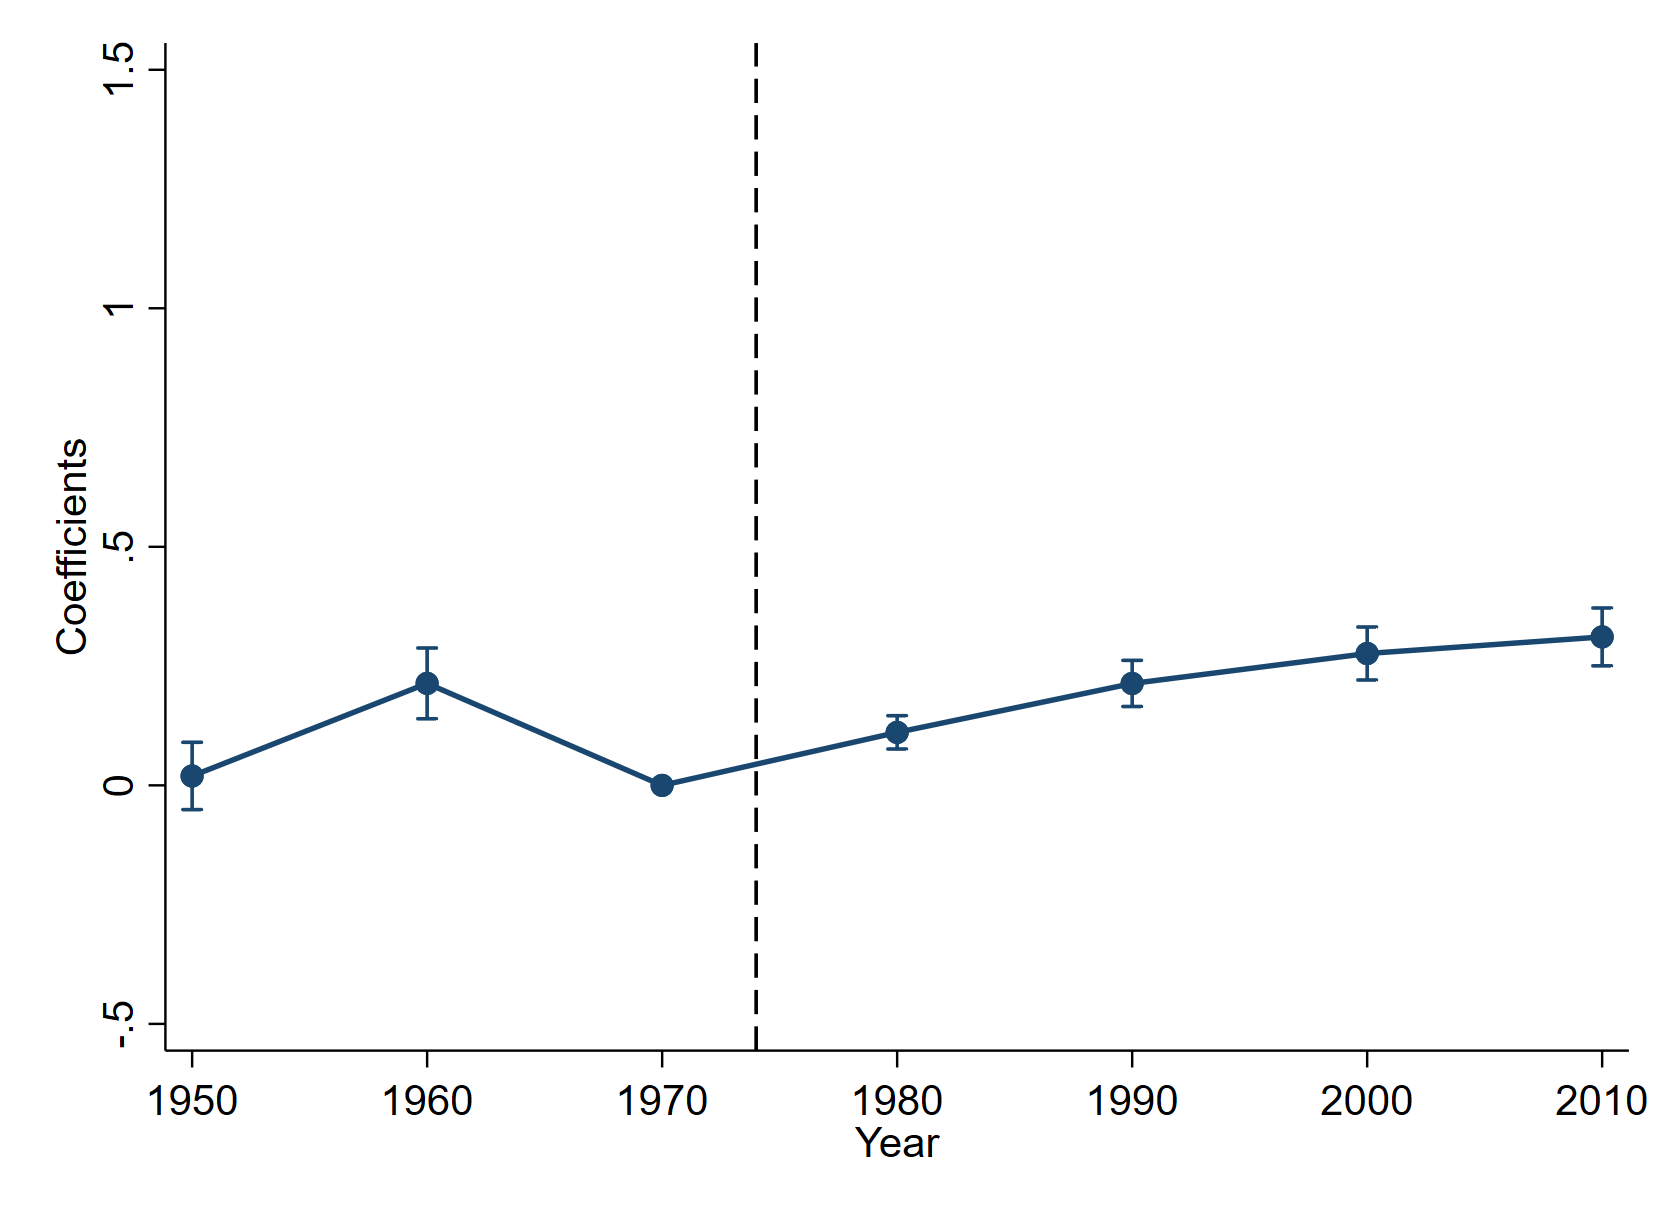
\includegraphics[width=\textwidth]{figures/appendix/urbshare_csdid.png}
    \end{subfigure}
\end{figure}

\clearpage
\begin{figure}[H]
    \centering
    \caption*{Appendix Figure 5: Time-varying effects on Population}
    
    \begin{subfigure}{0.50\textwidth}
        \centering
        \caption{TWFE}
        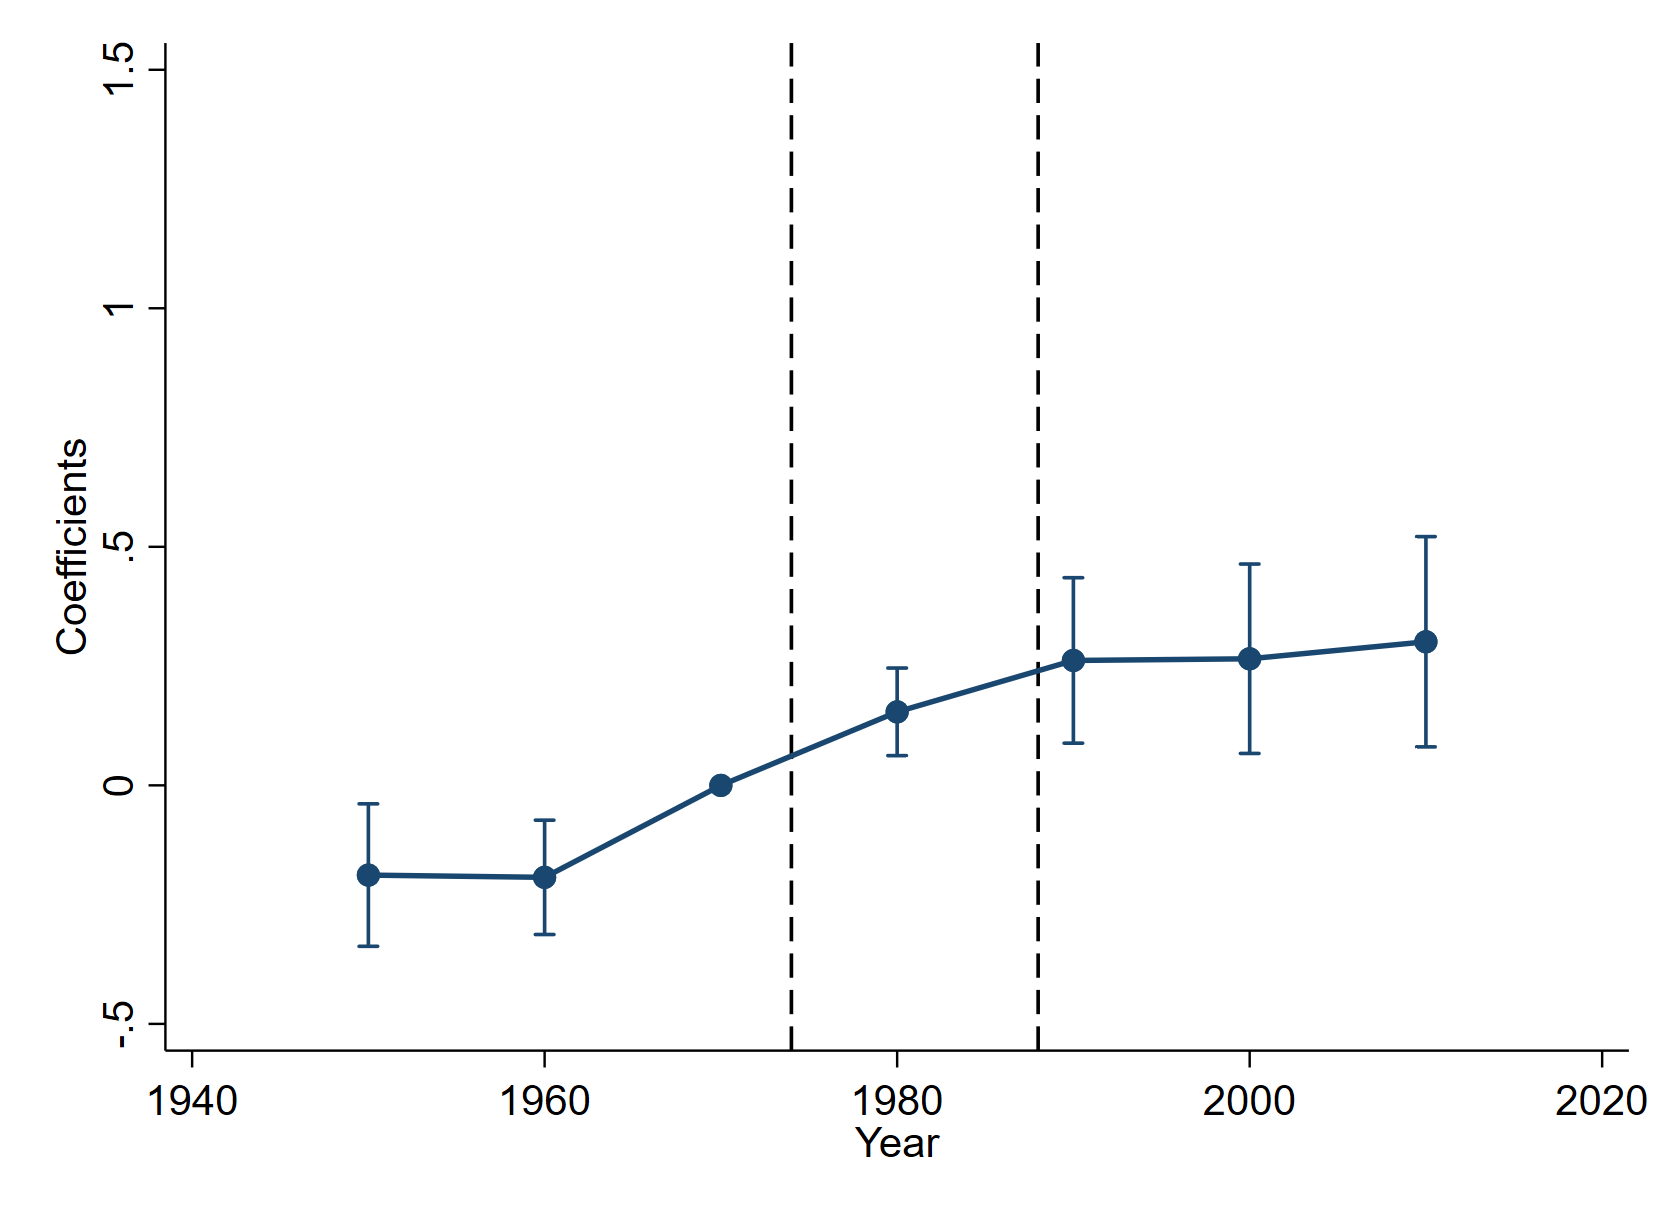
\includegraphics[width=\textwidth]{figures/pop.png}
 
    \end{subfigure}
    
    \begin{subfigure}{0.48\textwidth}
        \centering
        \caption{Borusyak et al (2022) Estimator}
        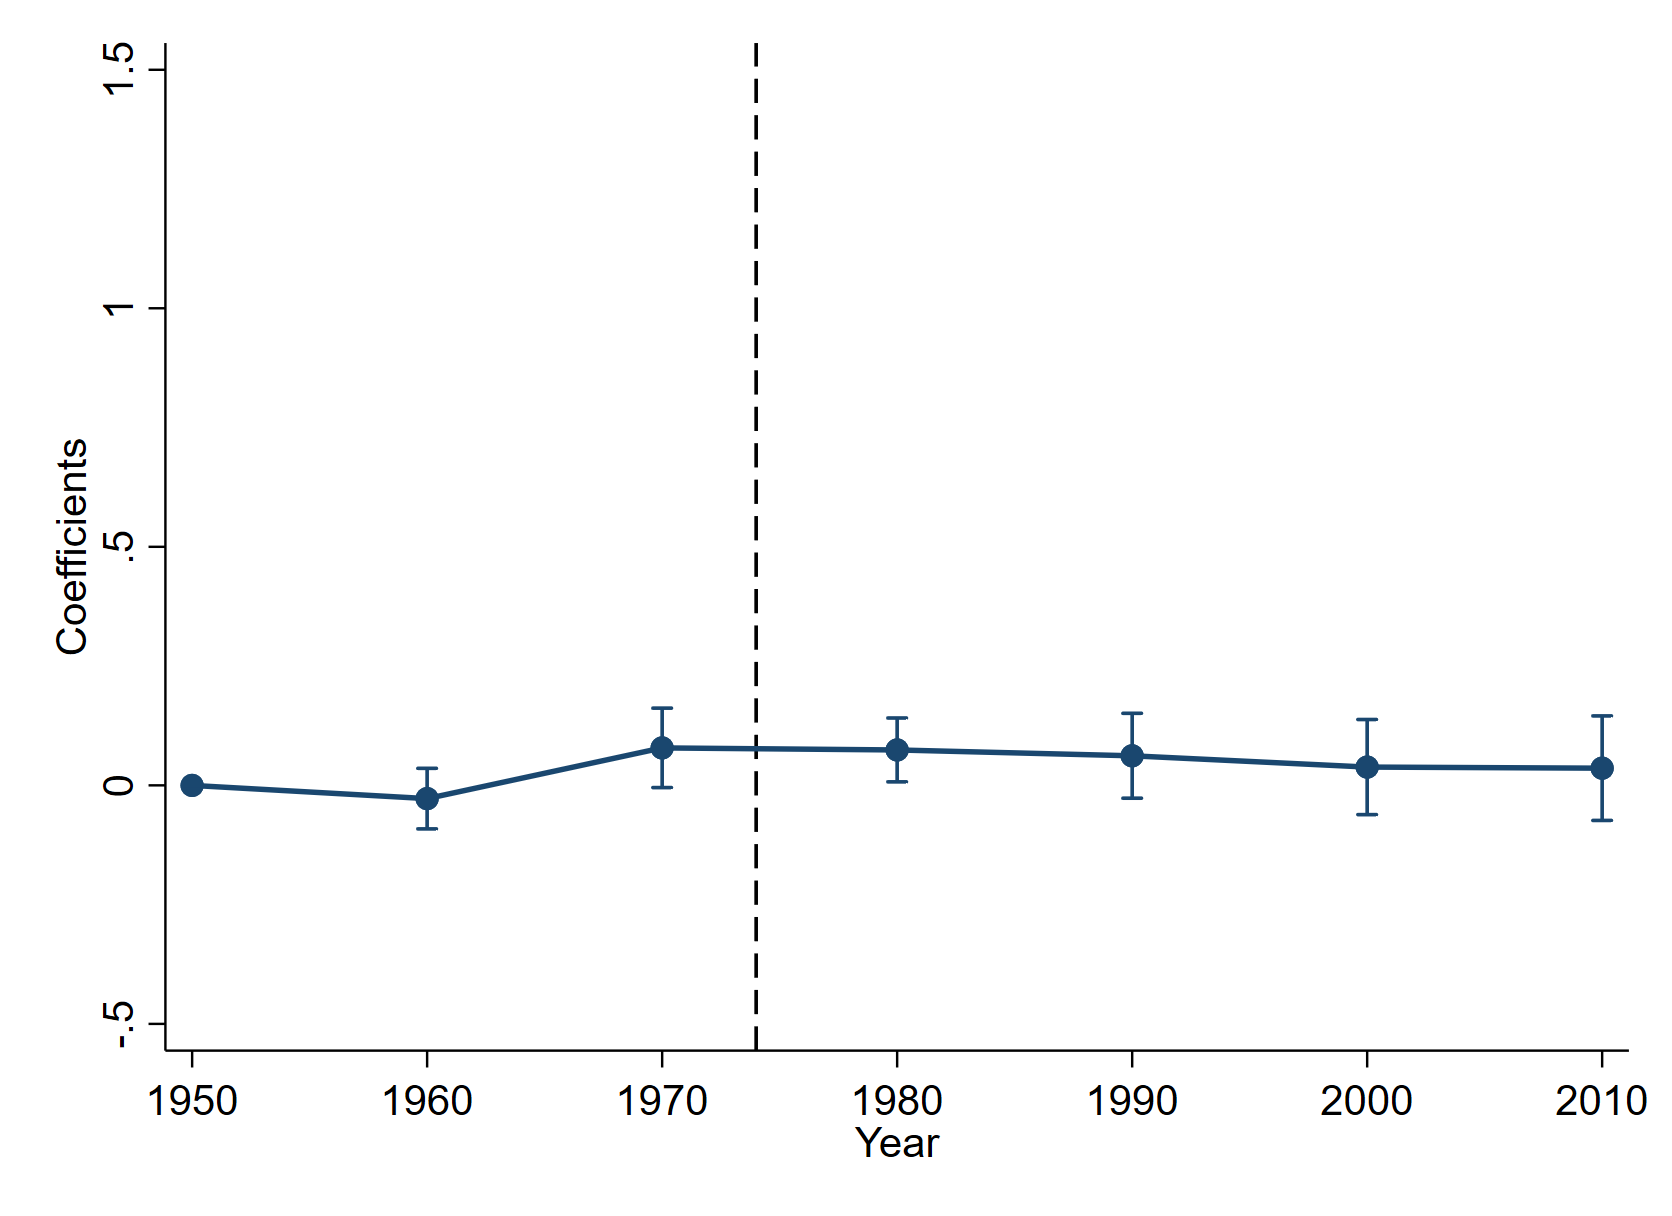
\includegraphics[width=\textwidth]{figures/appendix/pop_imputation.png}

    \end{subfigure}
    \begin{subfigure}{0.48\textwidth}
        \centering
        \caption{Callaway and Sant'Anna (2021) Estimator}
        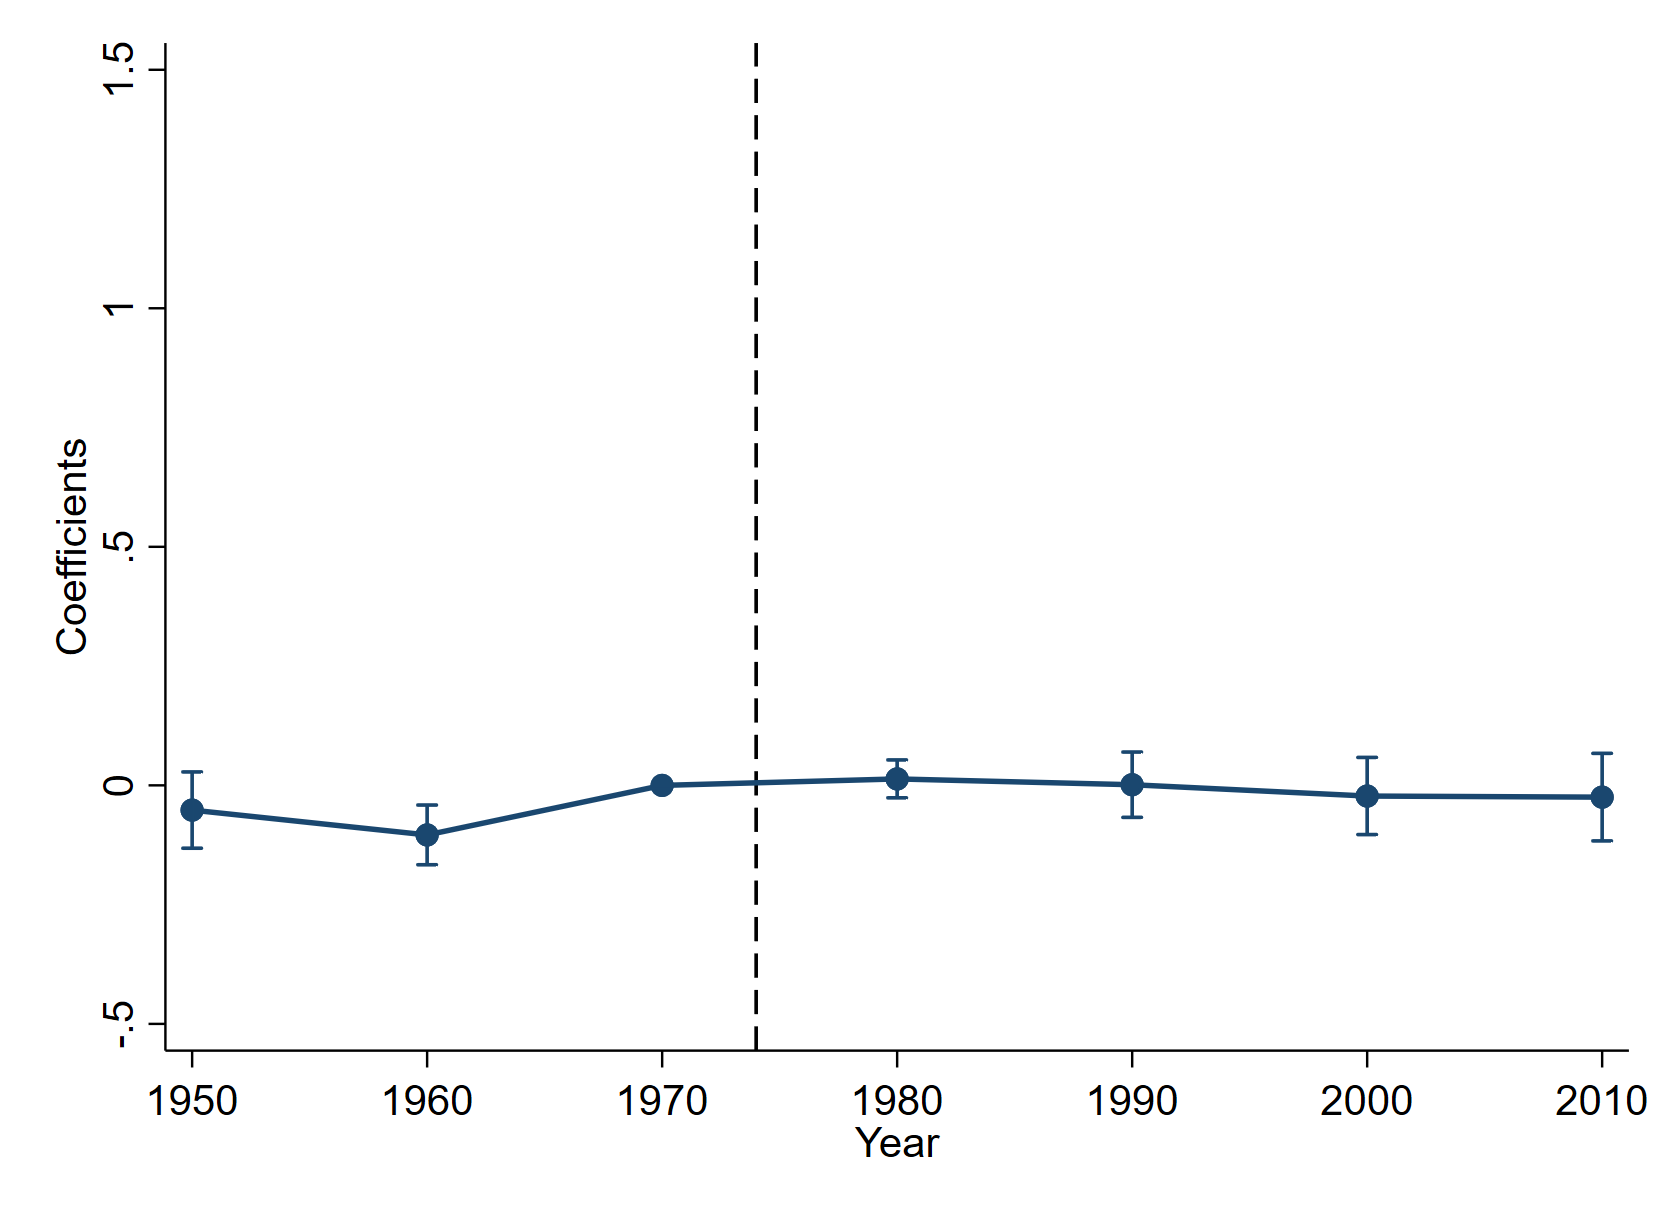
\includegraphics[width=\textwidth]{figures/appendix/pop_csdid.png}
    \end{subfigure}
\end{figure}

\clearpage
\begin{figure}[H]
    \centering
    \caption*{Appendix Figure 6: Urban Population Treatment Intensity}
    \begin{subfigure}{0.48\textwidth}
        \centering
        \caption{1970}
        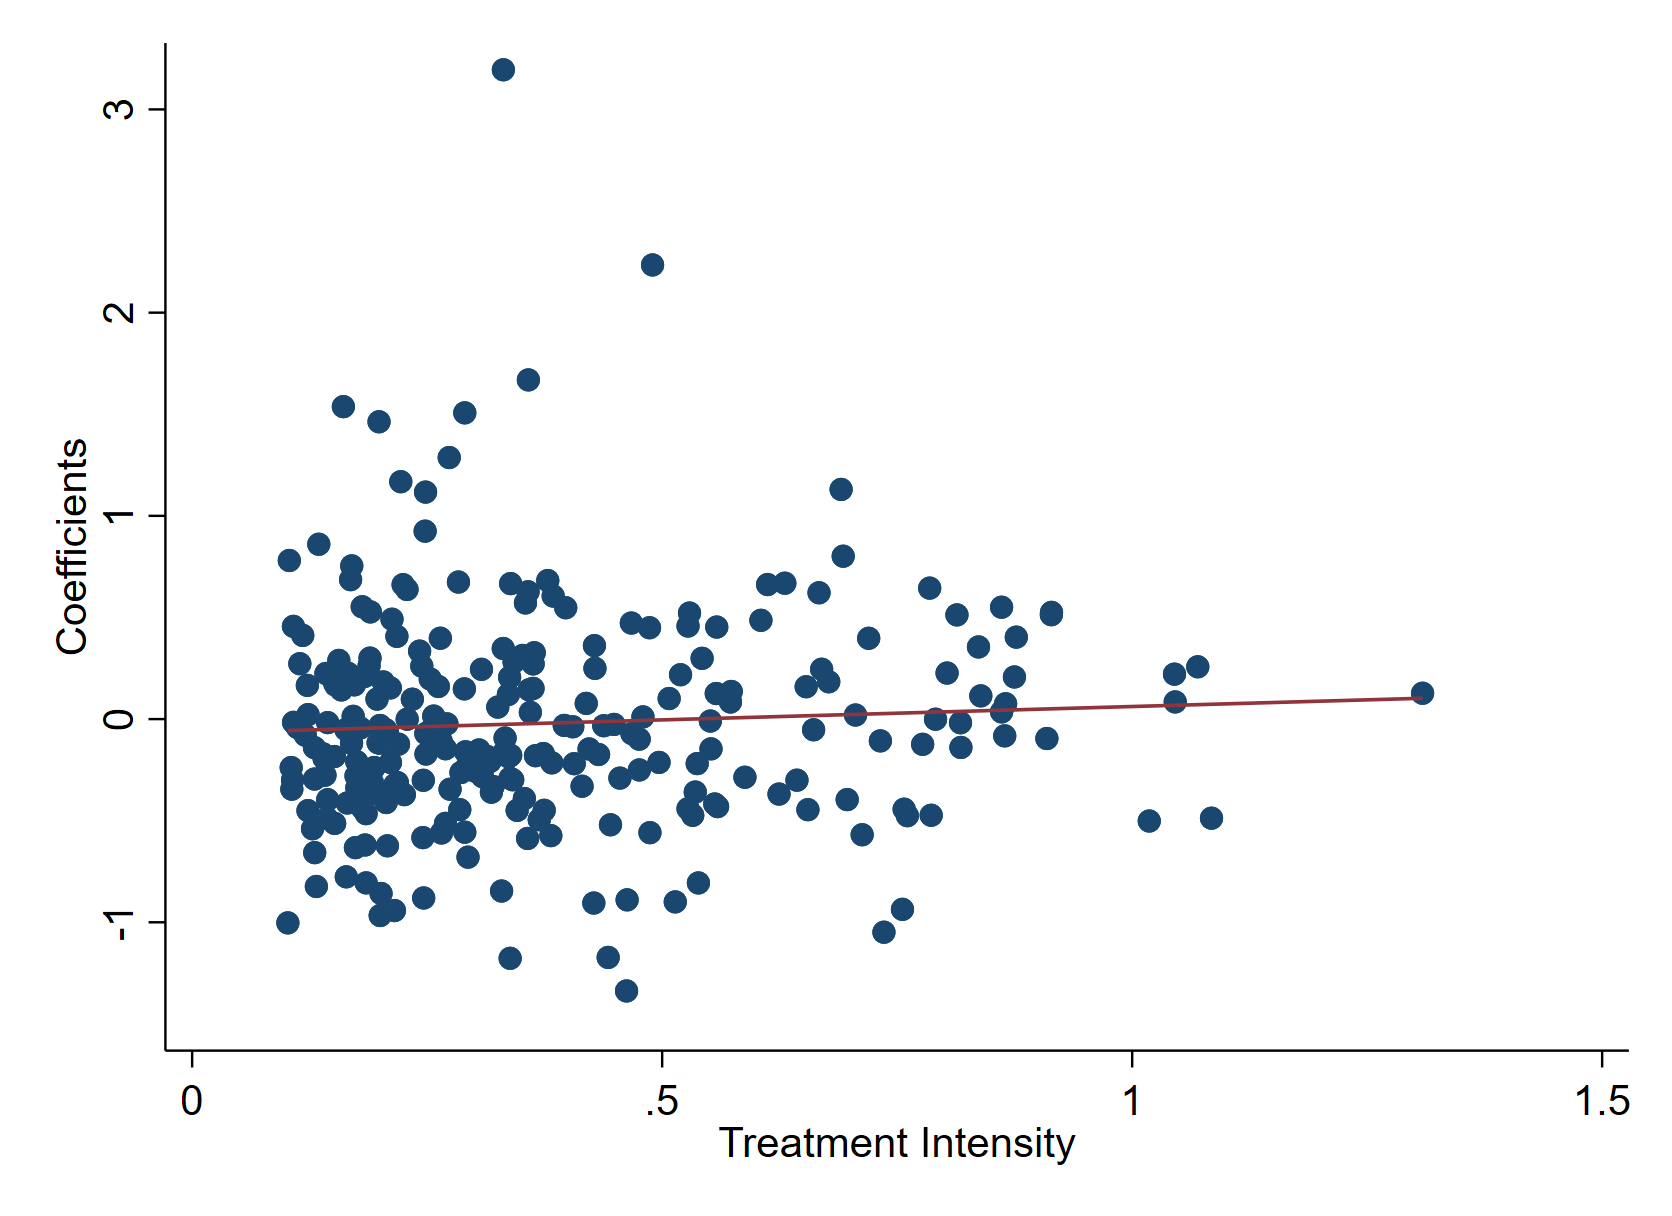
\includegraphics[width=\textwidth]{figures/appendix/urbpop_treatment_intensity_1970.png}
    \end{subfigure}
    \begin{subfigure}{0.48\textwidth}
        \centering
        \caption{1980}
        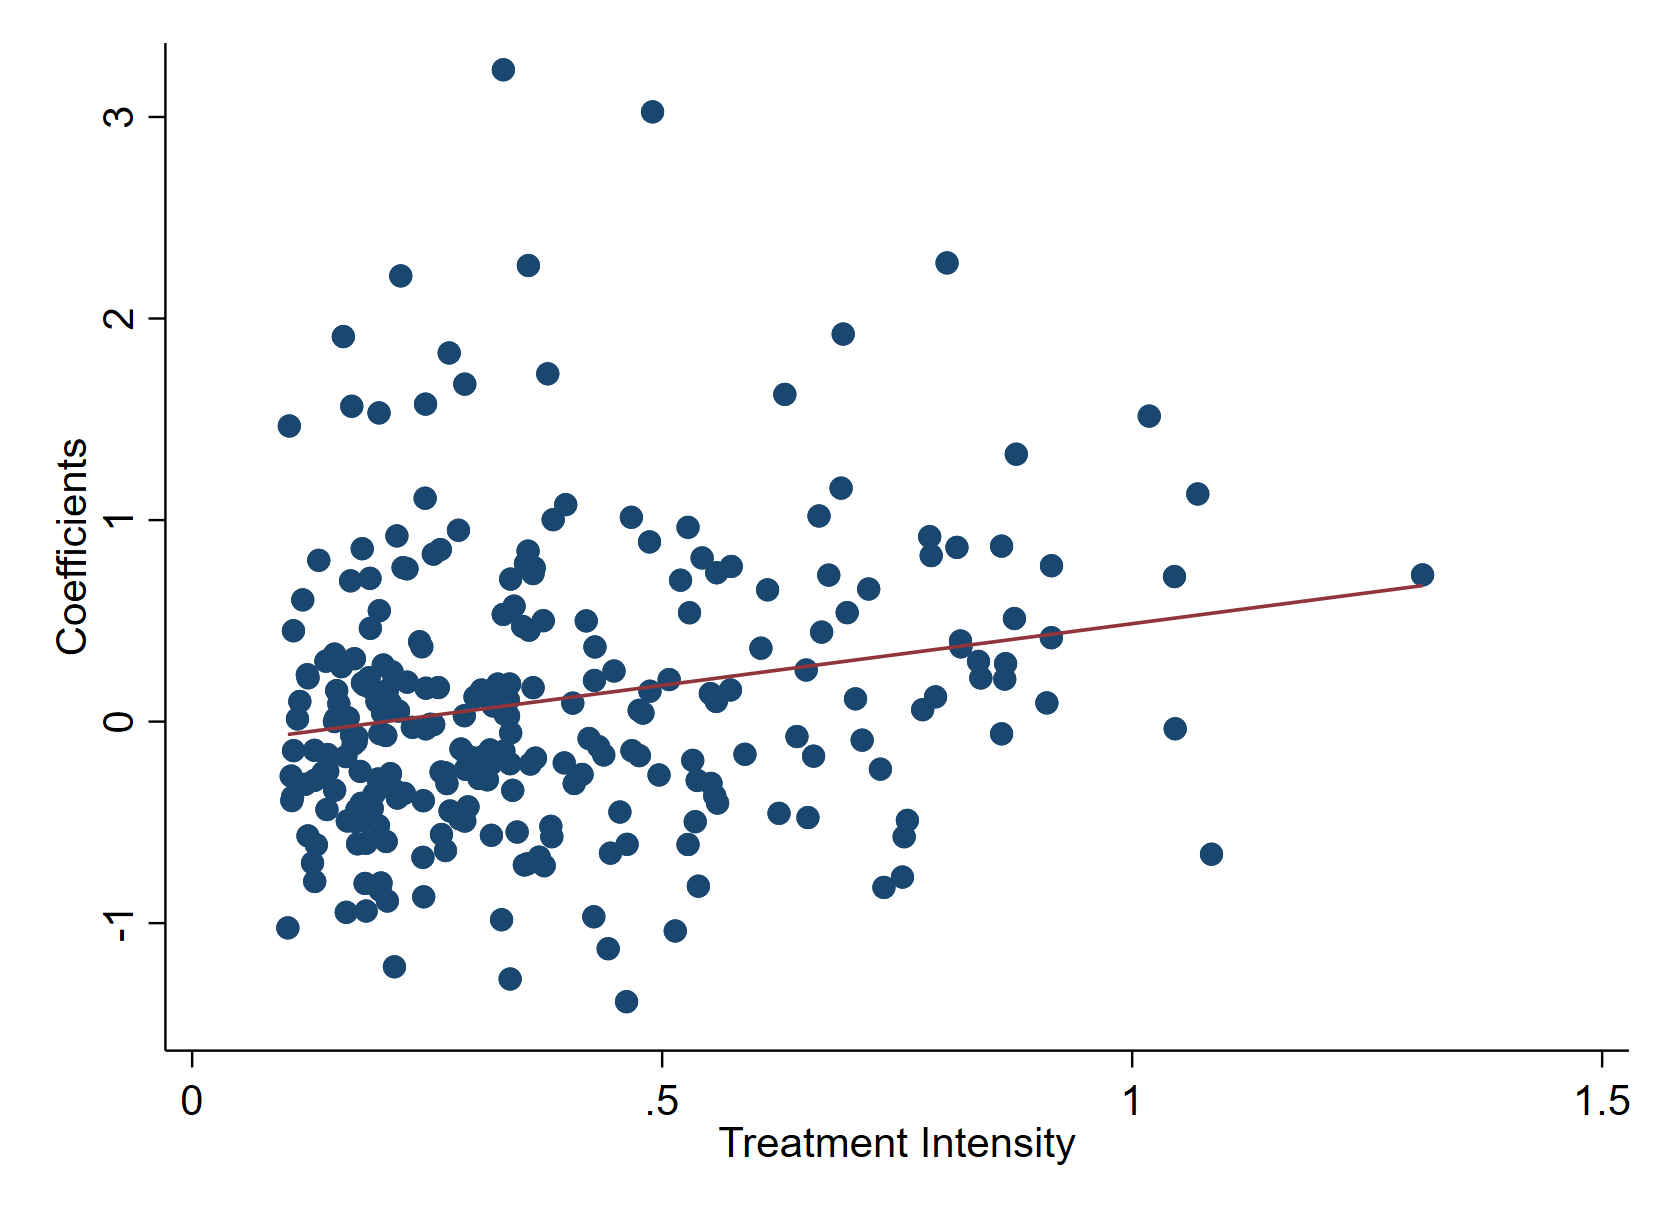
\includegraphics[width=\textwidth]{figures/appendix/urbpop_treatment_intensity_1980.png}
    \end{subfigure}
    \hfill
    \begin{subfigure}{0.48\textwidth}
        \centering
        \caption{1990}
        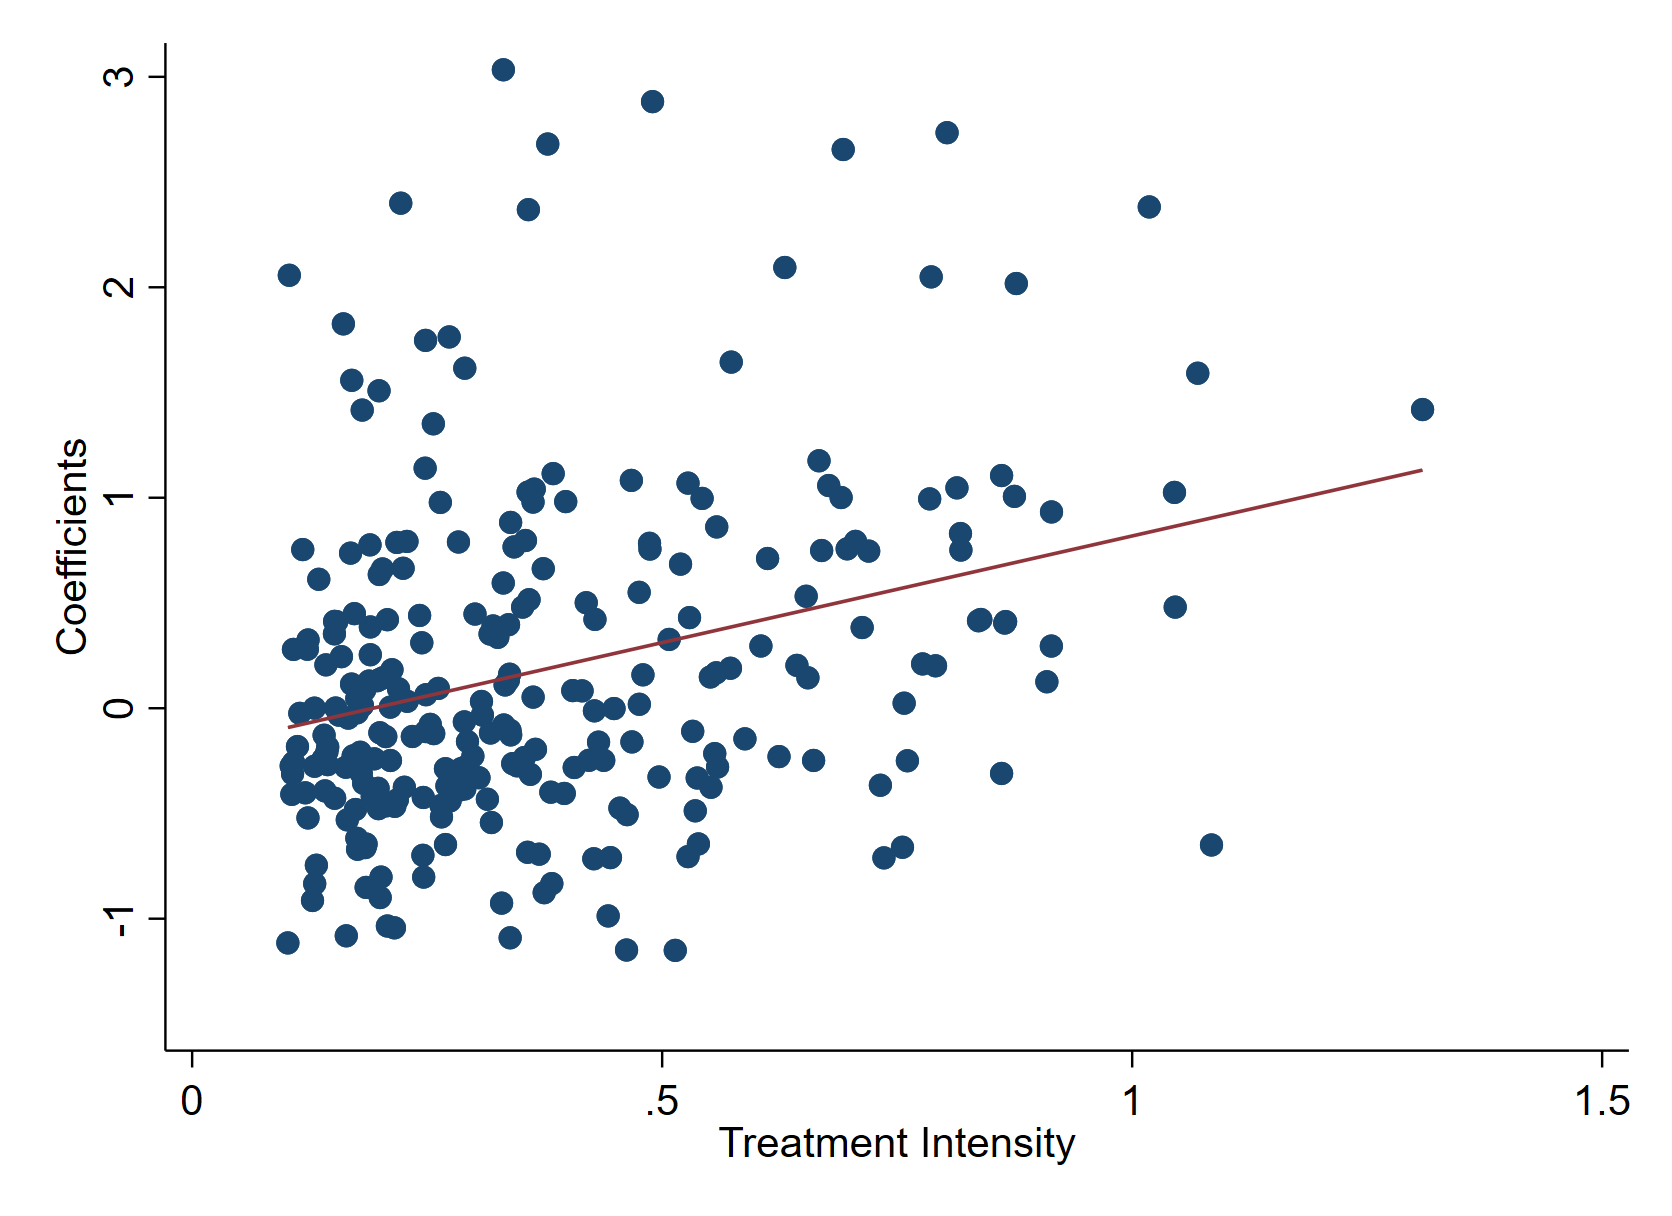
\includegraphics[width=\textwidth]{figures/appendix/urbpop_treatment_intensity_1990.png}
    \end{subfigure}
    \hfill
    \begin{subfigure}{0.48\textwidth}
        \centering
        \caption{2000}
        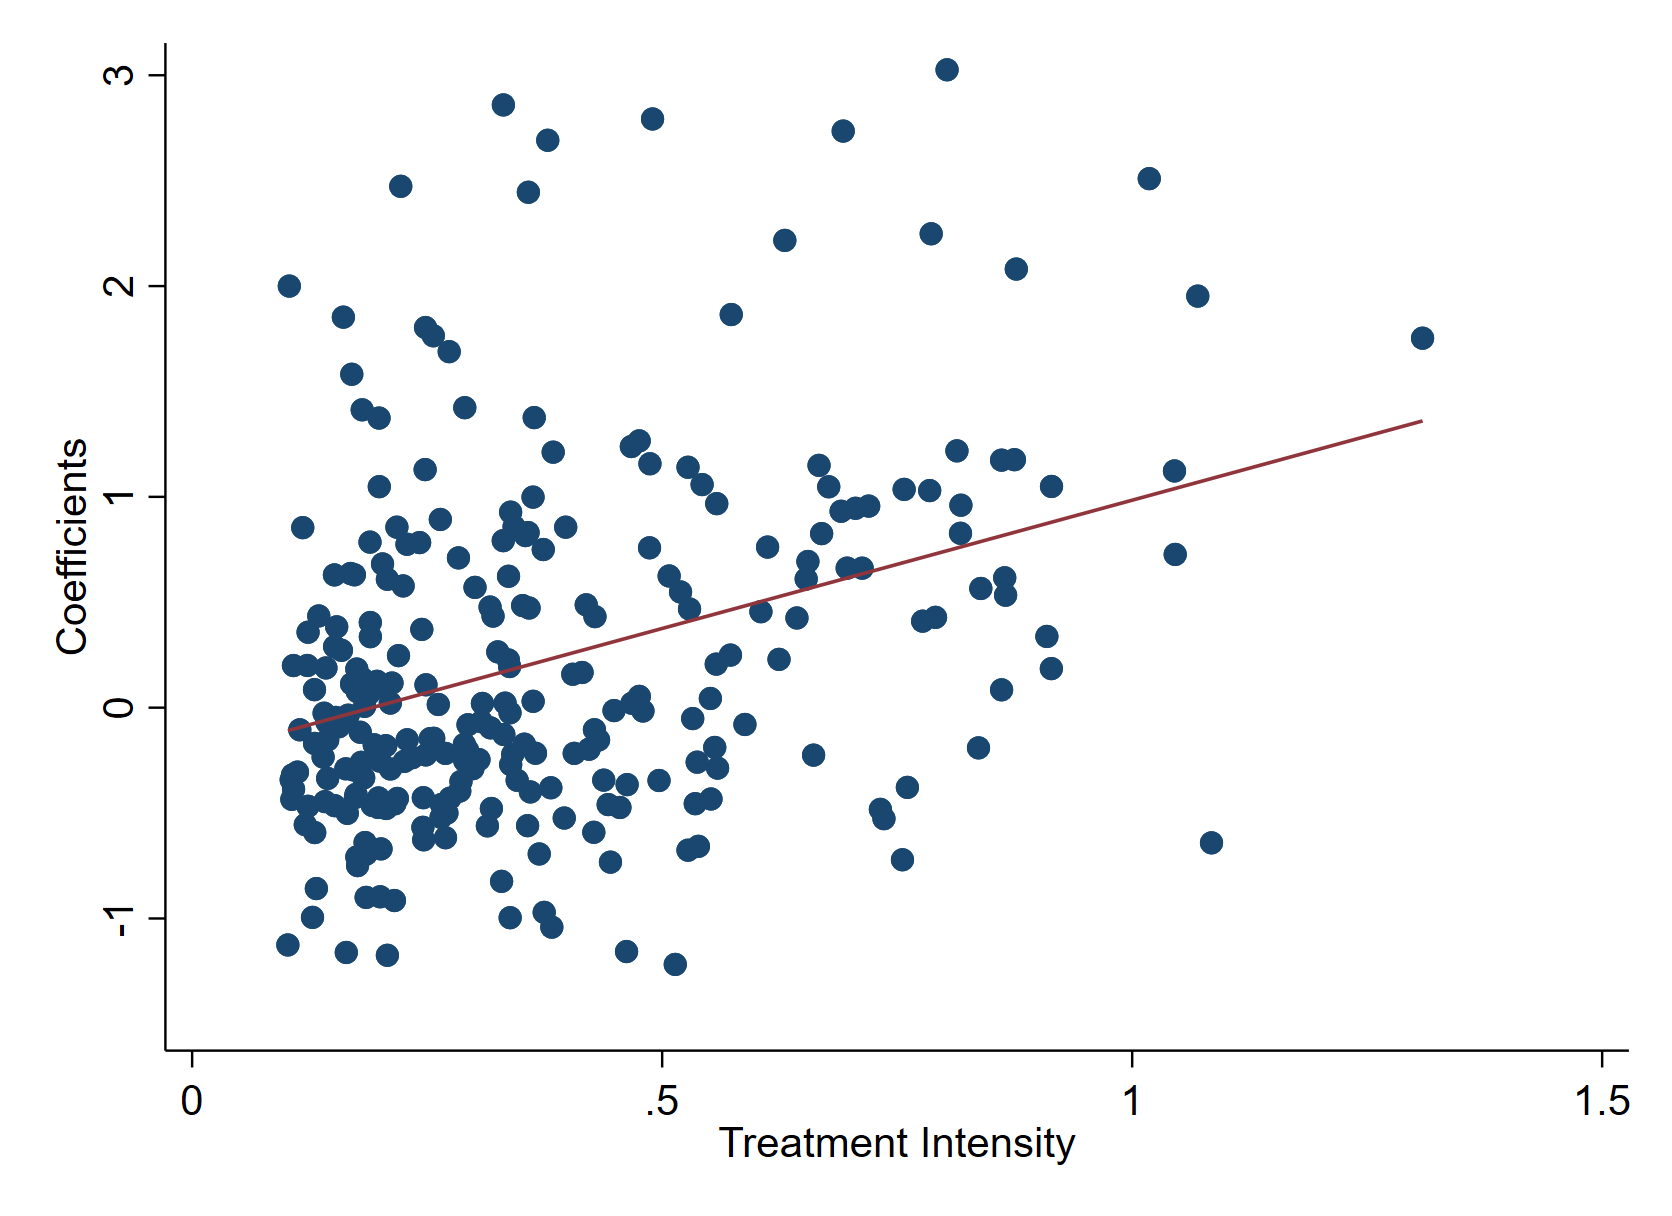
\includegraphics[width=\textwidth]{figures/appendix/urbpop_treatment_intensity_2000.png}
    \end{subfigure}
    \hfill
    \begin{subfigure}{0.48\textwidth}
        \centering
        \caption{2010}
        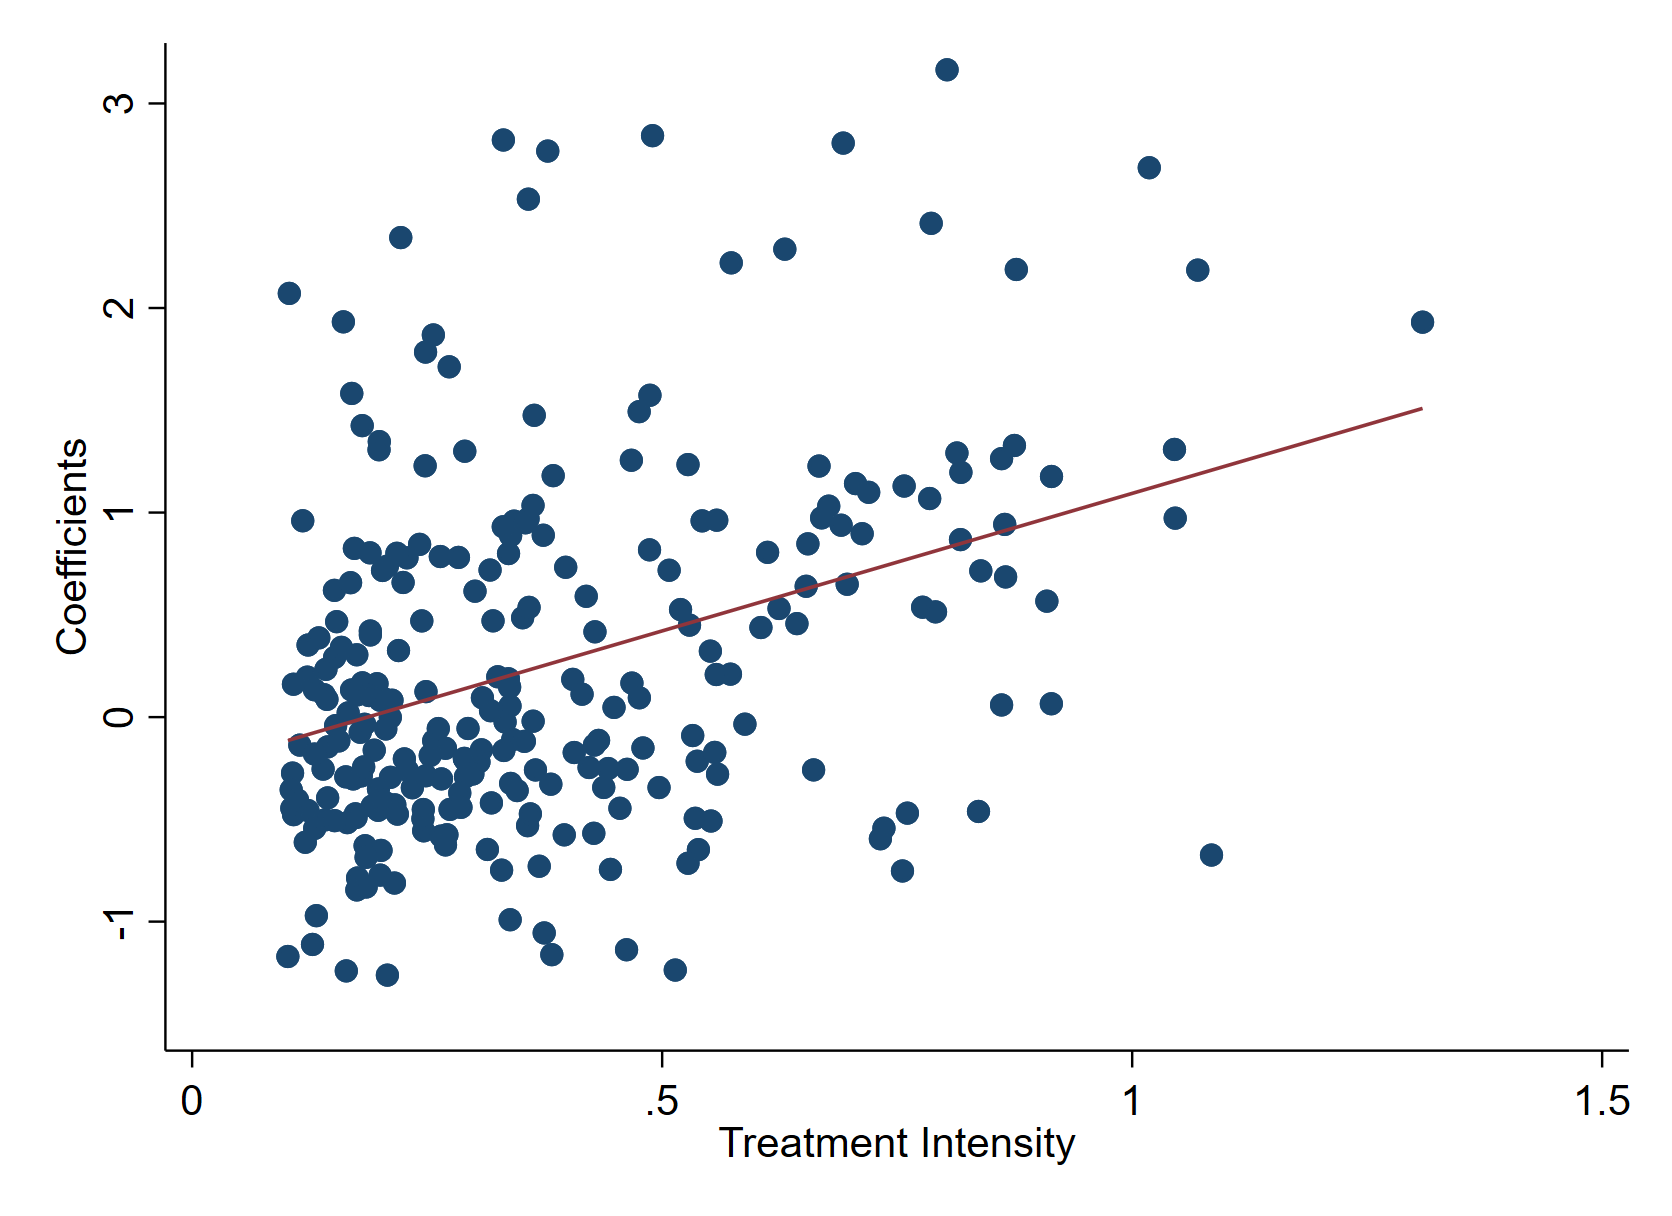
\includegraphics[width=\textwidth]{figures/appendix/urbpop_treatment_intensity_2010.png}
    \end{subfigure}
\end{figure}

\clearpage
\begin{figure}[H]
    \centering
    \caption*{Appendix Figure 7: Urban Population Share Treatment Intensity}
    \begin{subfigure}{0.48\textwidth}
        \centering
        \caption{1970}
        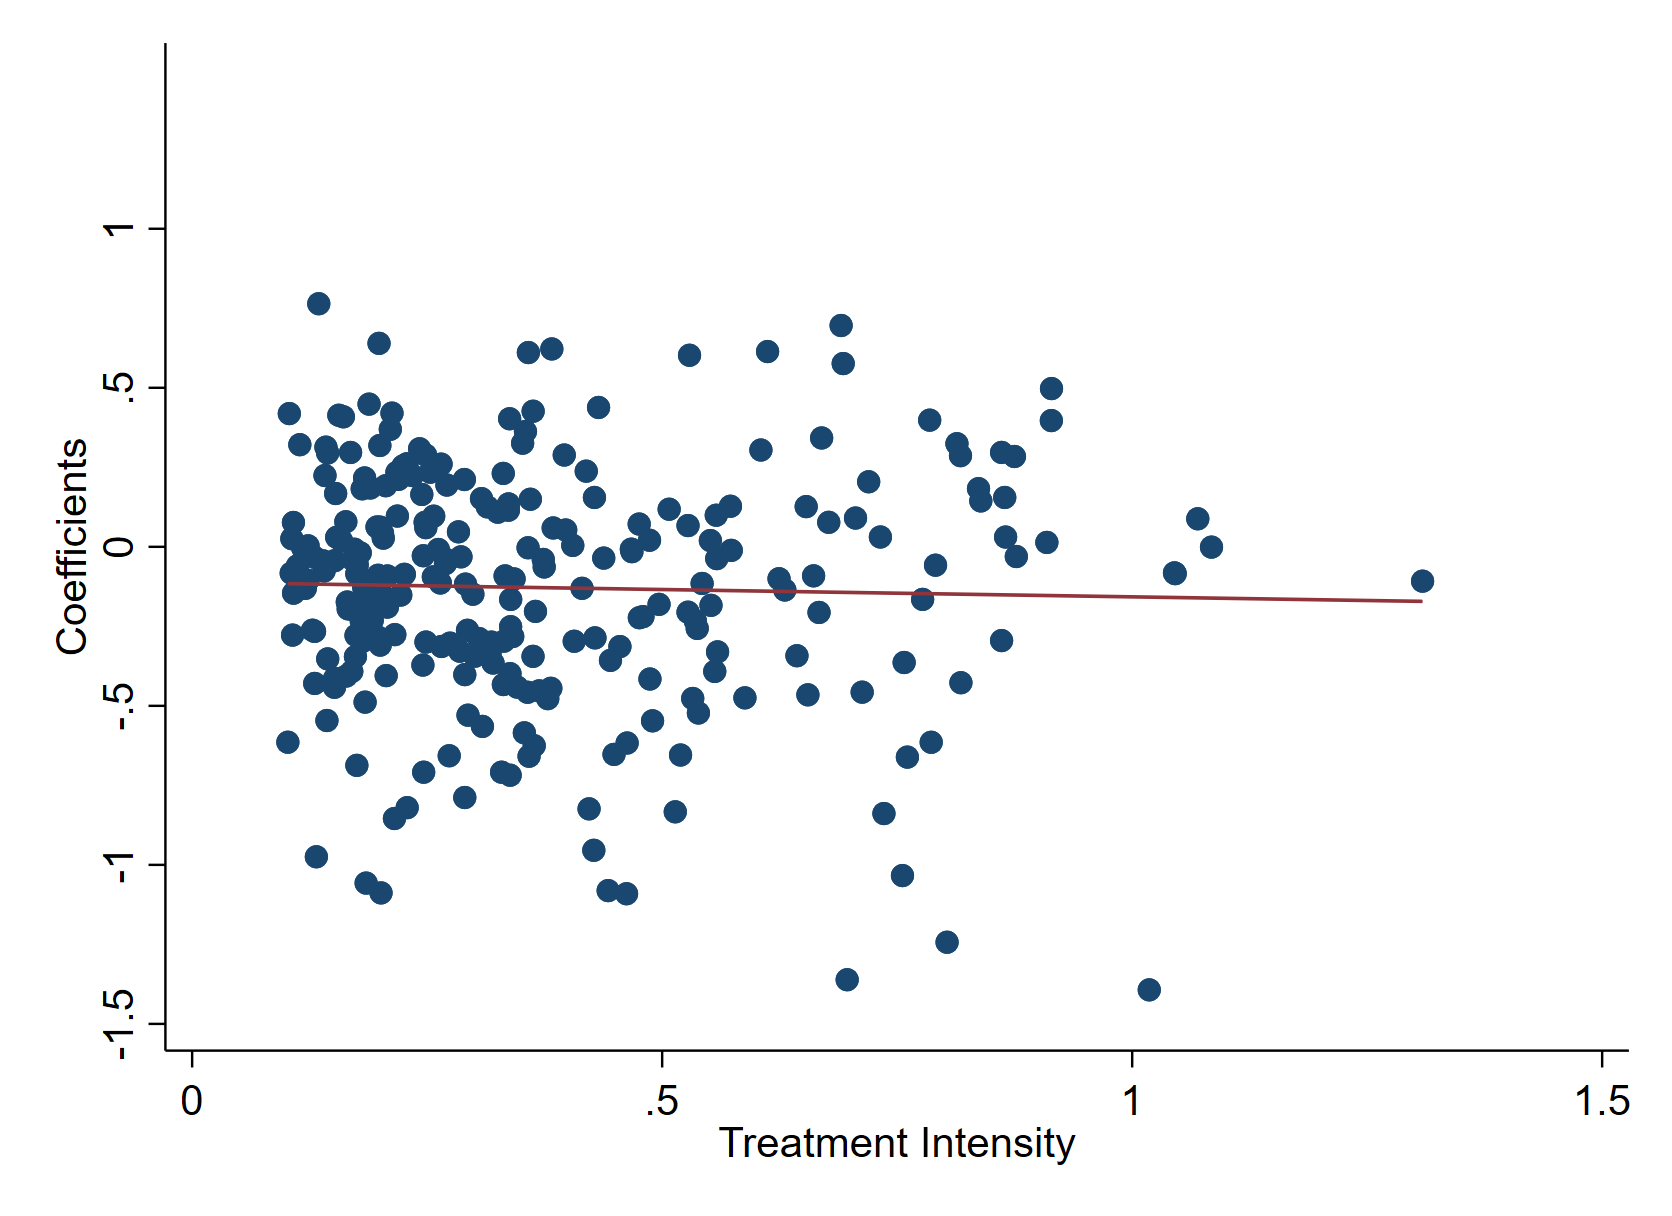
\includegraphics[width=\textwidth]{figures/appendix/urbshare_treatment_intensity_1970.png}
    \end{subfigure}
    \begin{subfigure}{0.48\textwidth}
        \centering
        \caption{1980}
        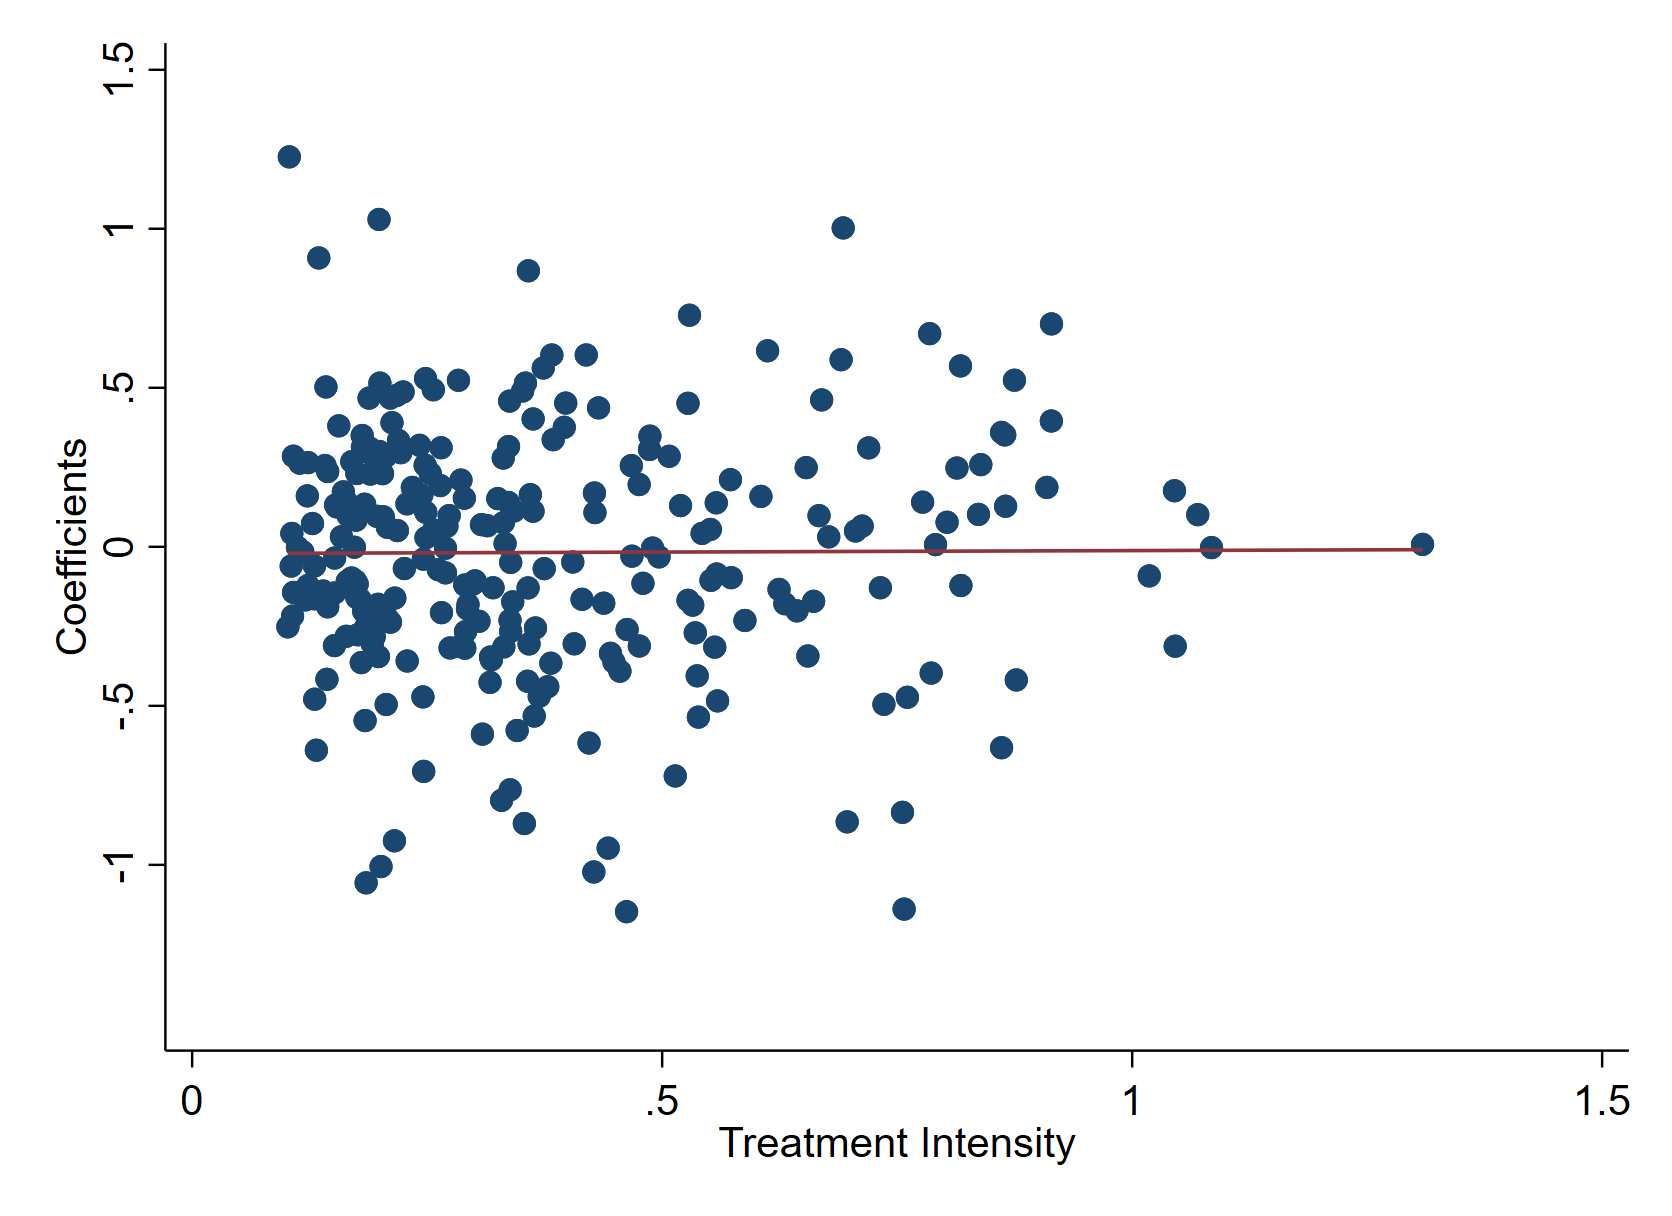
\includegraphics[width=\textwidth]{figures/appendix/urbshare_treatment_intensity_1980.png}
    \end{subfigure}
    \hfill
    \begin{subfigure}{0.48\textwidth}
        \centering
        \caption{1990}
        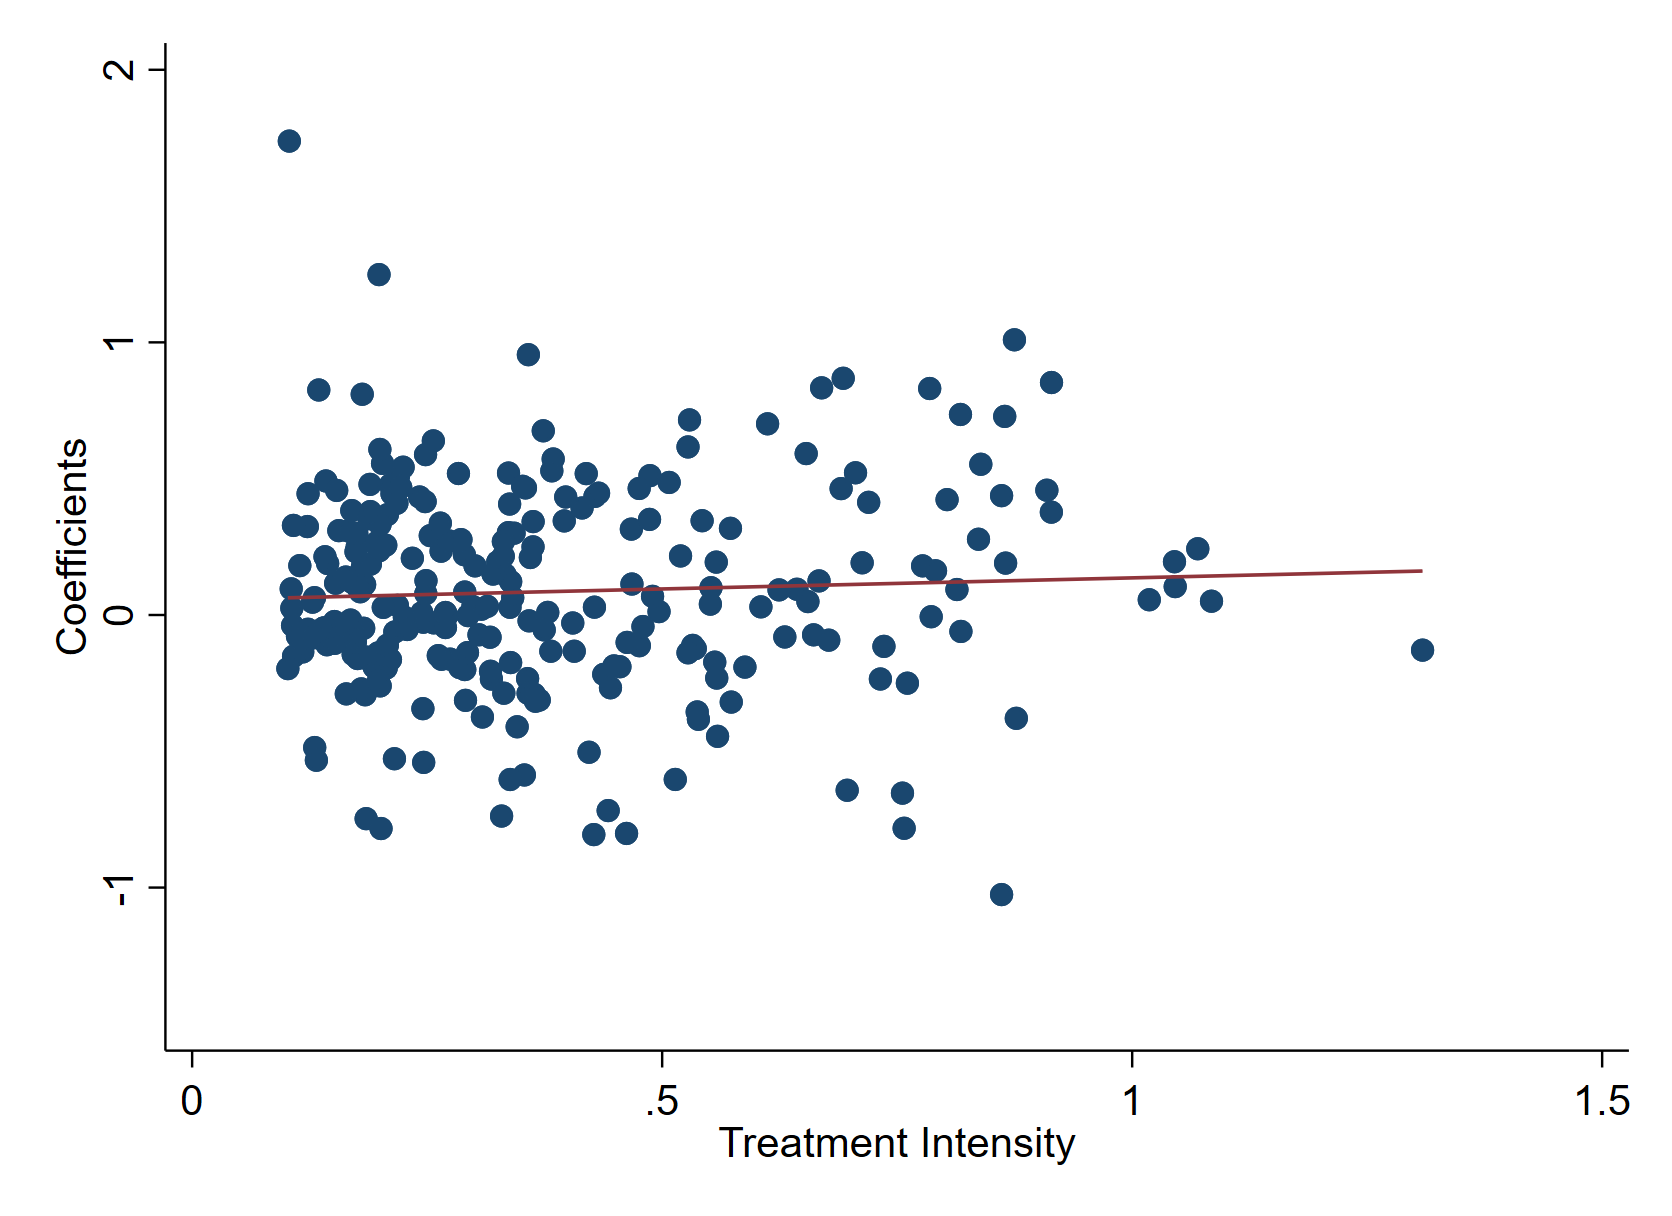
\includegraphics[width=\textwidth]{figures/appendix/urbshare_treatment_intensity_1990.png}
    \end{subfigure}
    \hfill
    \begin{subfigure}{0.48\textwidth}
        \centering
        \caption{2000}
        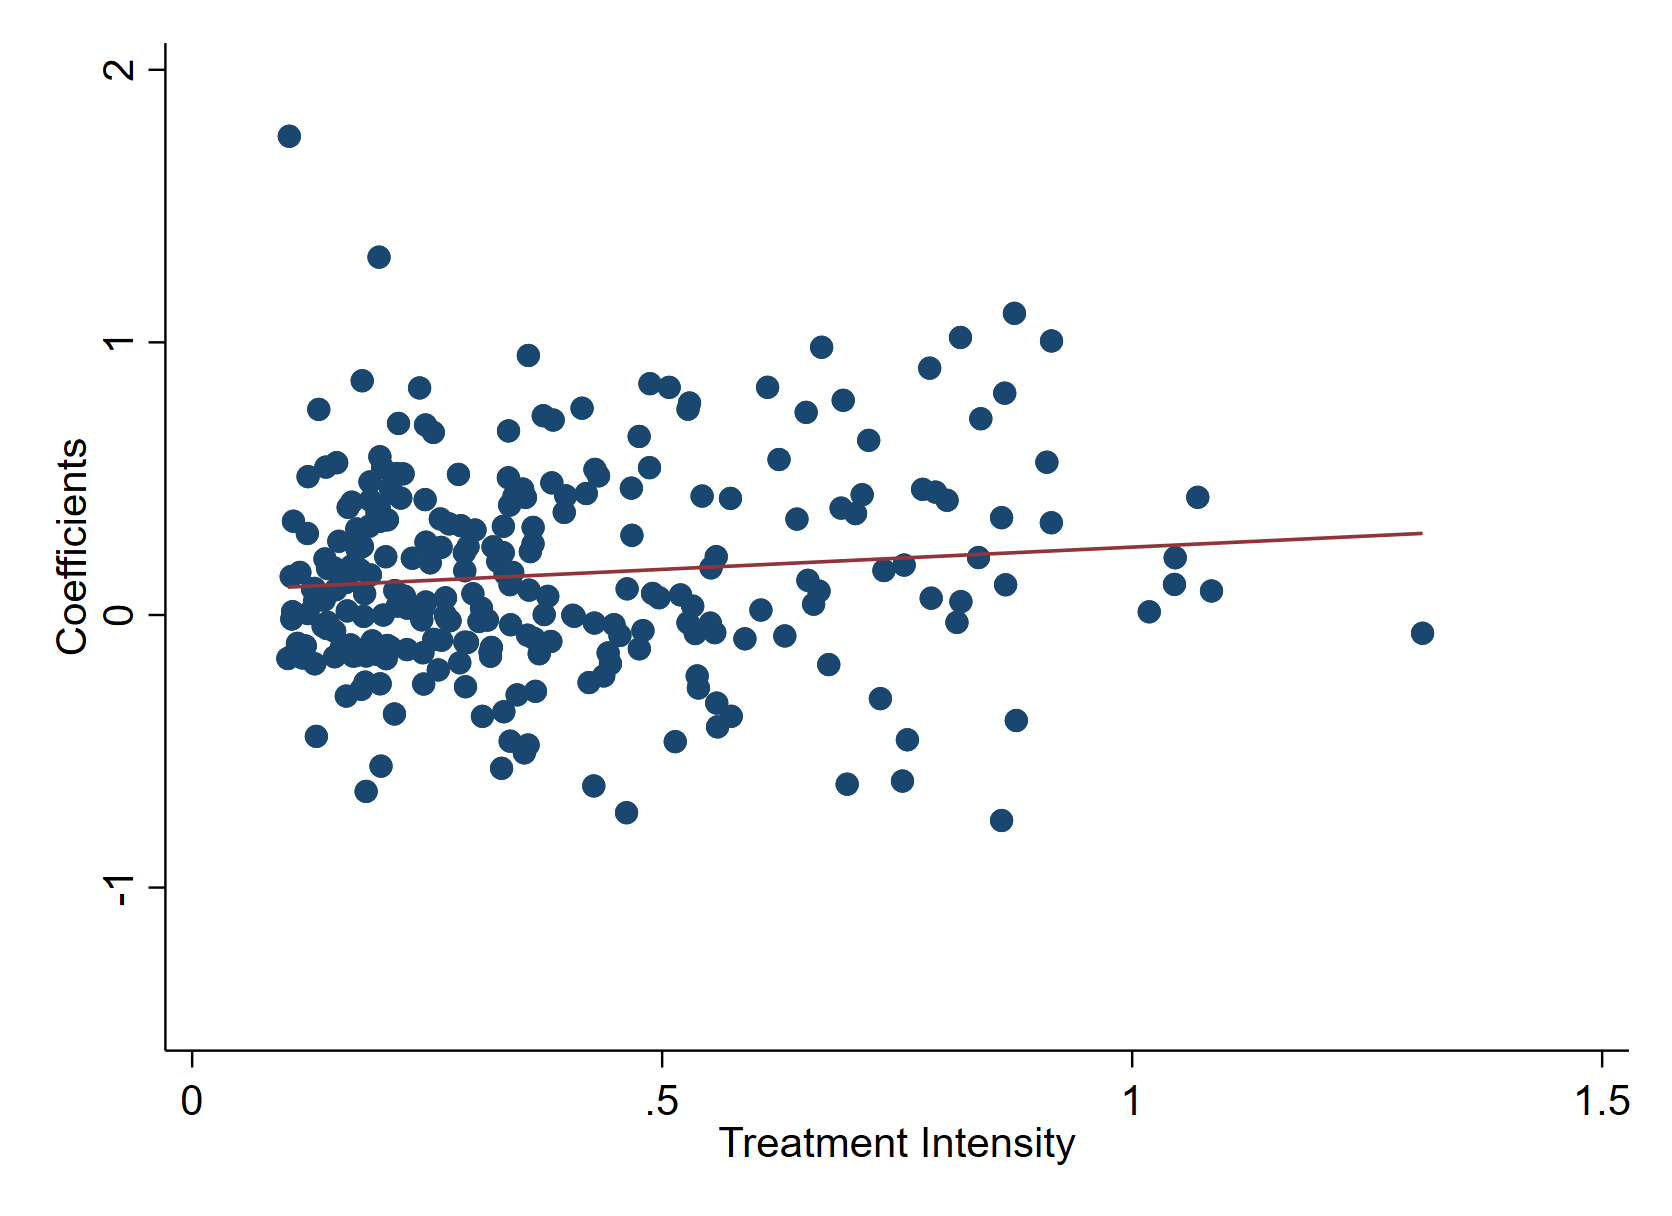
\includegraphics[width=\textwidth]{figures/appendix/urbshare_treatment_intensity_2000.png}
    \end{subfigure}
    \hfill
    \begin{subfigure}{0.48\textwidth}
        \centering
        \caption{2010}
        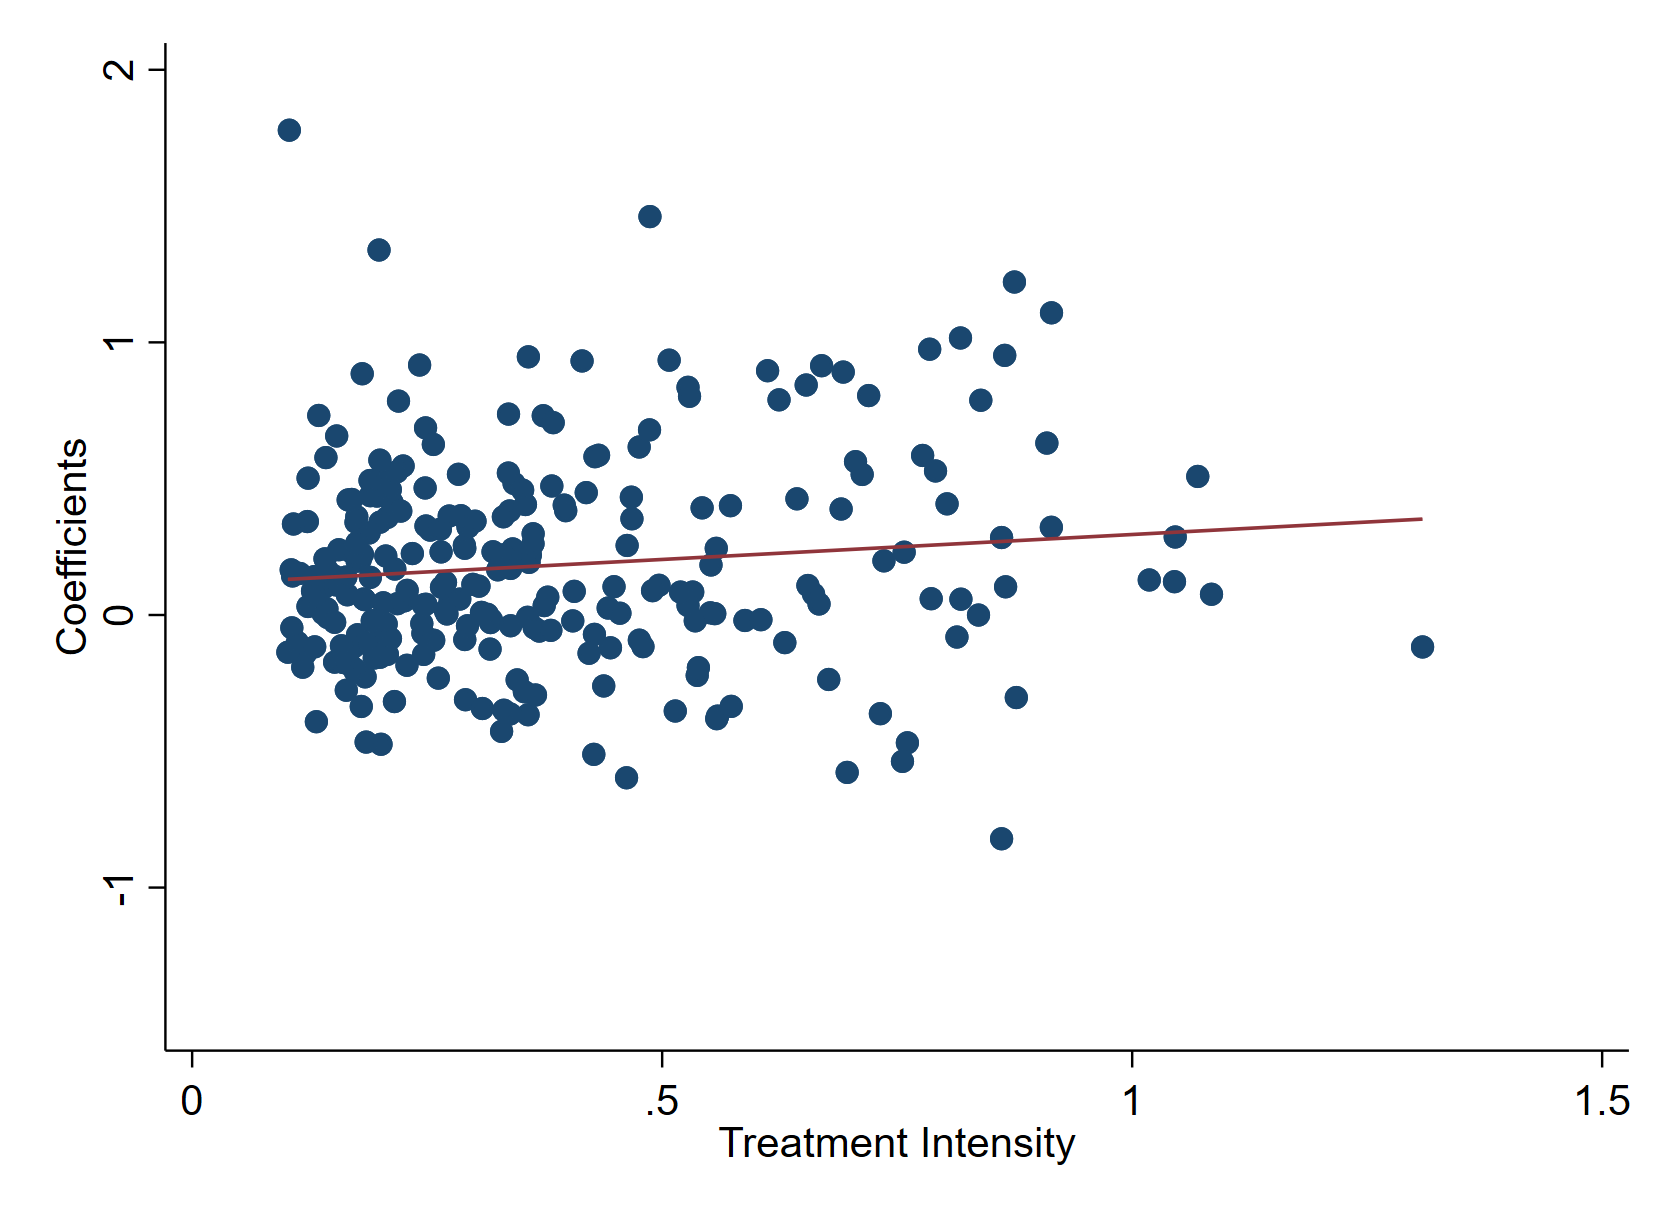
\includegraphics[width=\textwidth]{figures/appendix/urbshare_treatment_intensity_2010.png}
    \end{subfigure}
\end{figure}

\clearpage
\begin{figure}[H]
    \centering
    \caption*{Appendix Figure 8: Population Treatment Intensity}
    \begin{subfigure}{0.48\textwidth}
        \centering
        \caption{1970}
        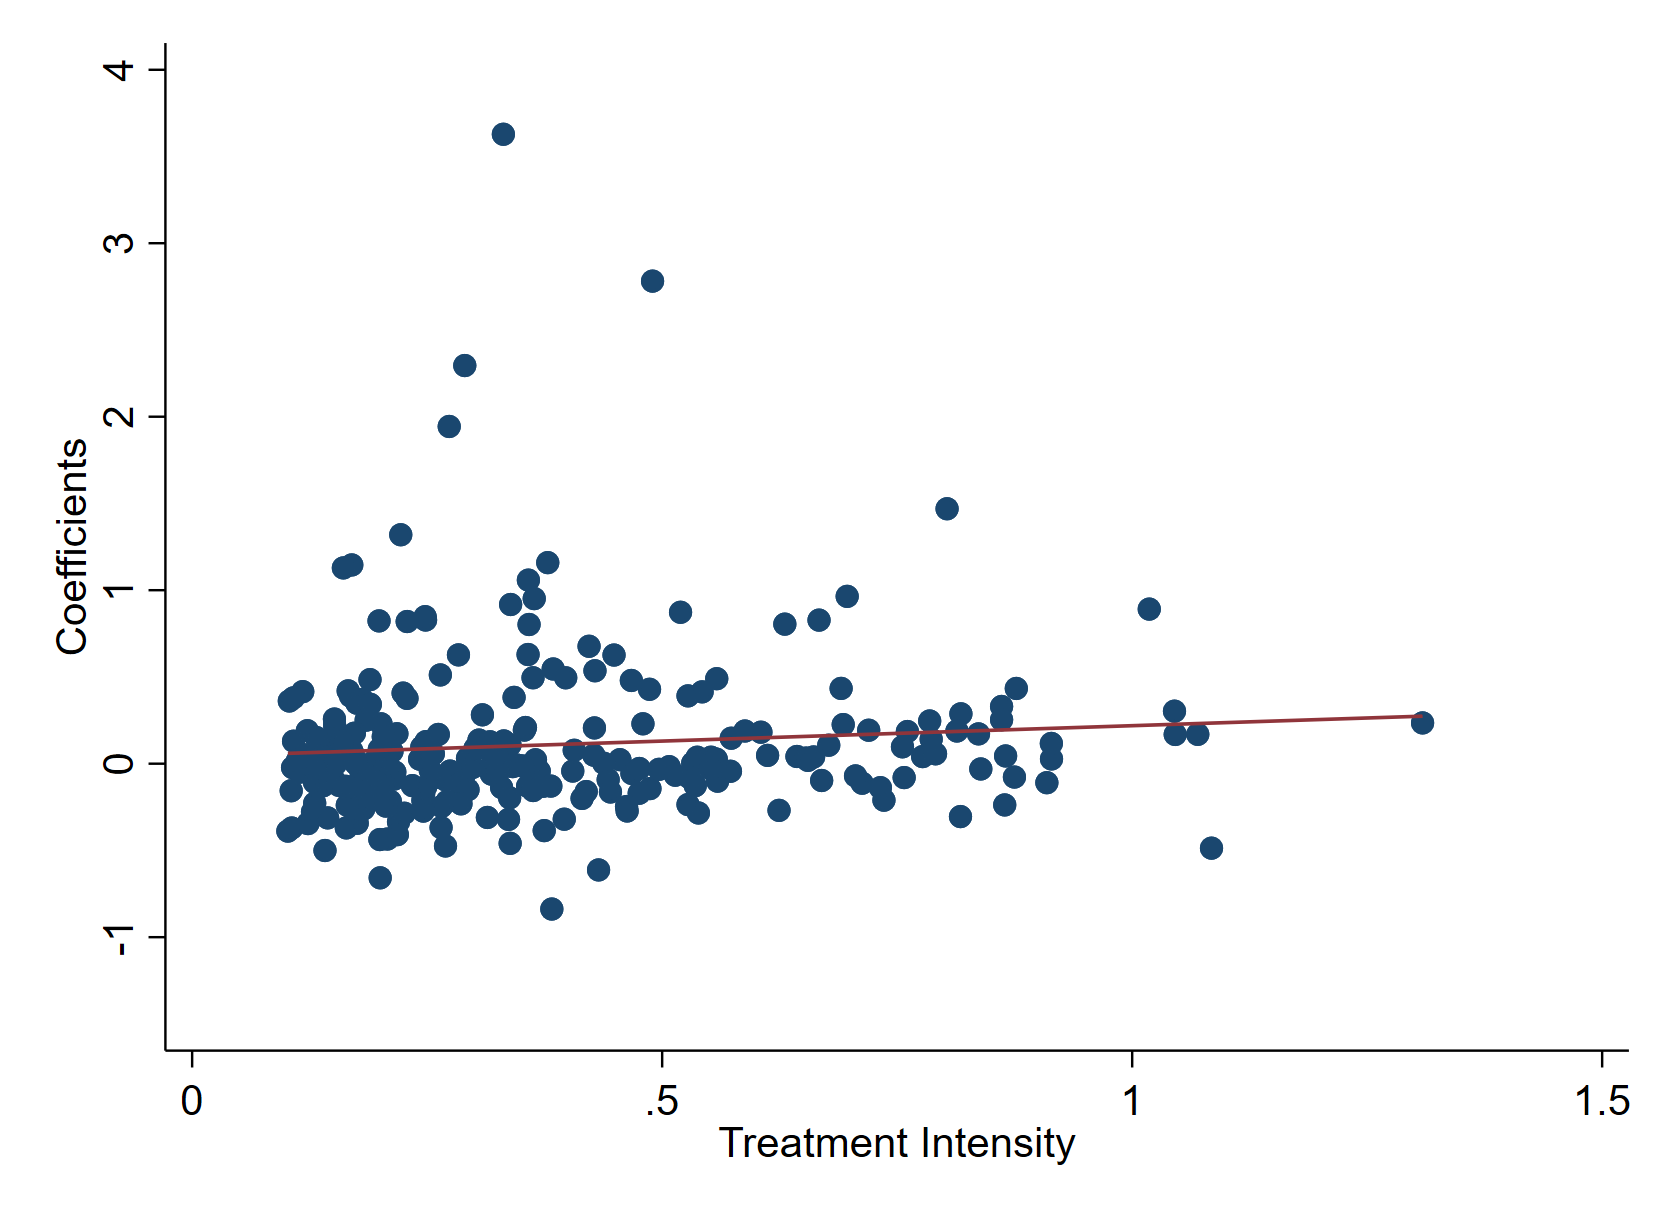
\includegraphics[width=\textwidth]{figures/appendix/pop_treatment_intensity_1970.png}
    \end{subfigure}
    \begin{subfigure}{0.48\textwidth}
        \centering
        \caption{1980}
        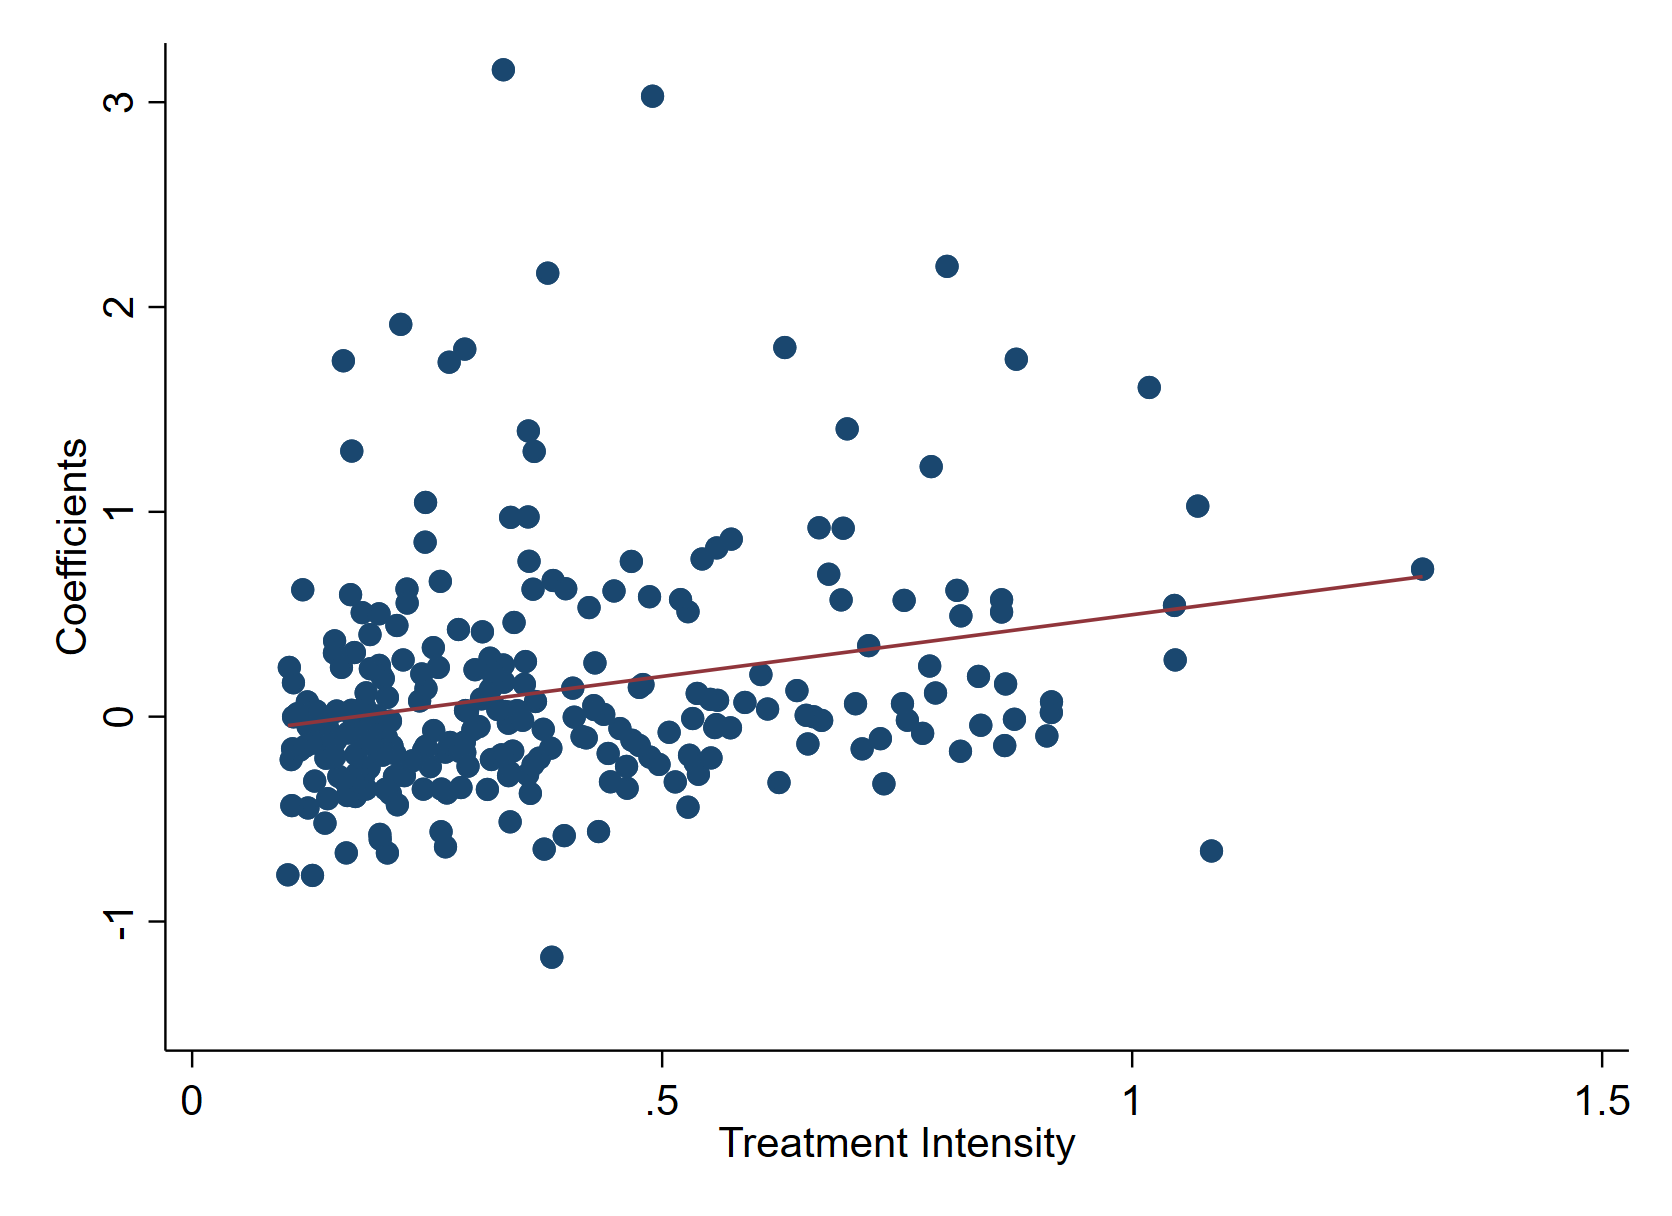
\includegraphics[width=\textwidth]{figures/appendix/pop_treatment_intensity_1980.png}
    \end{subfigure}
    \hfill
    \begin{subfigure}{0.48\textwidth}
        \centering
        \caption{1990}
        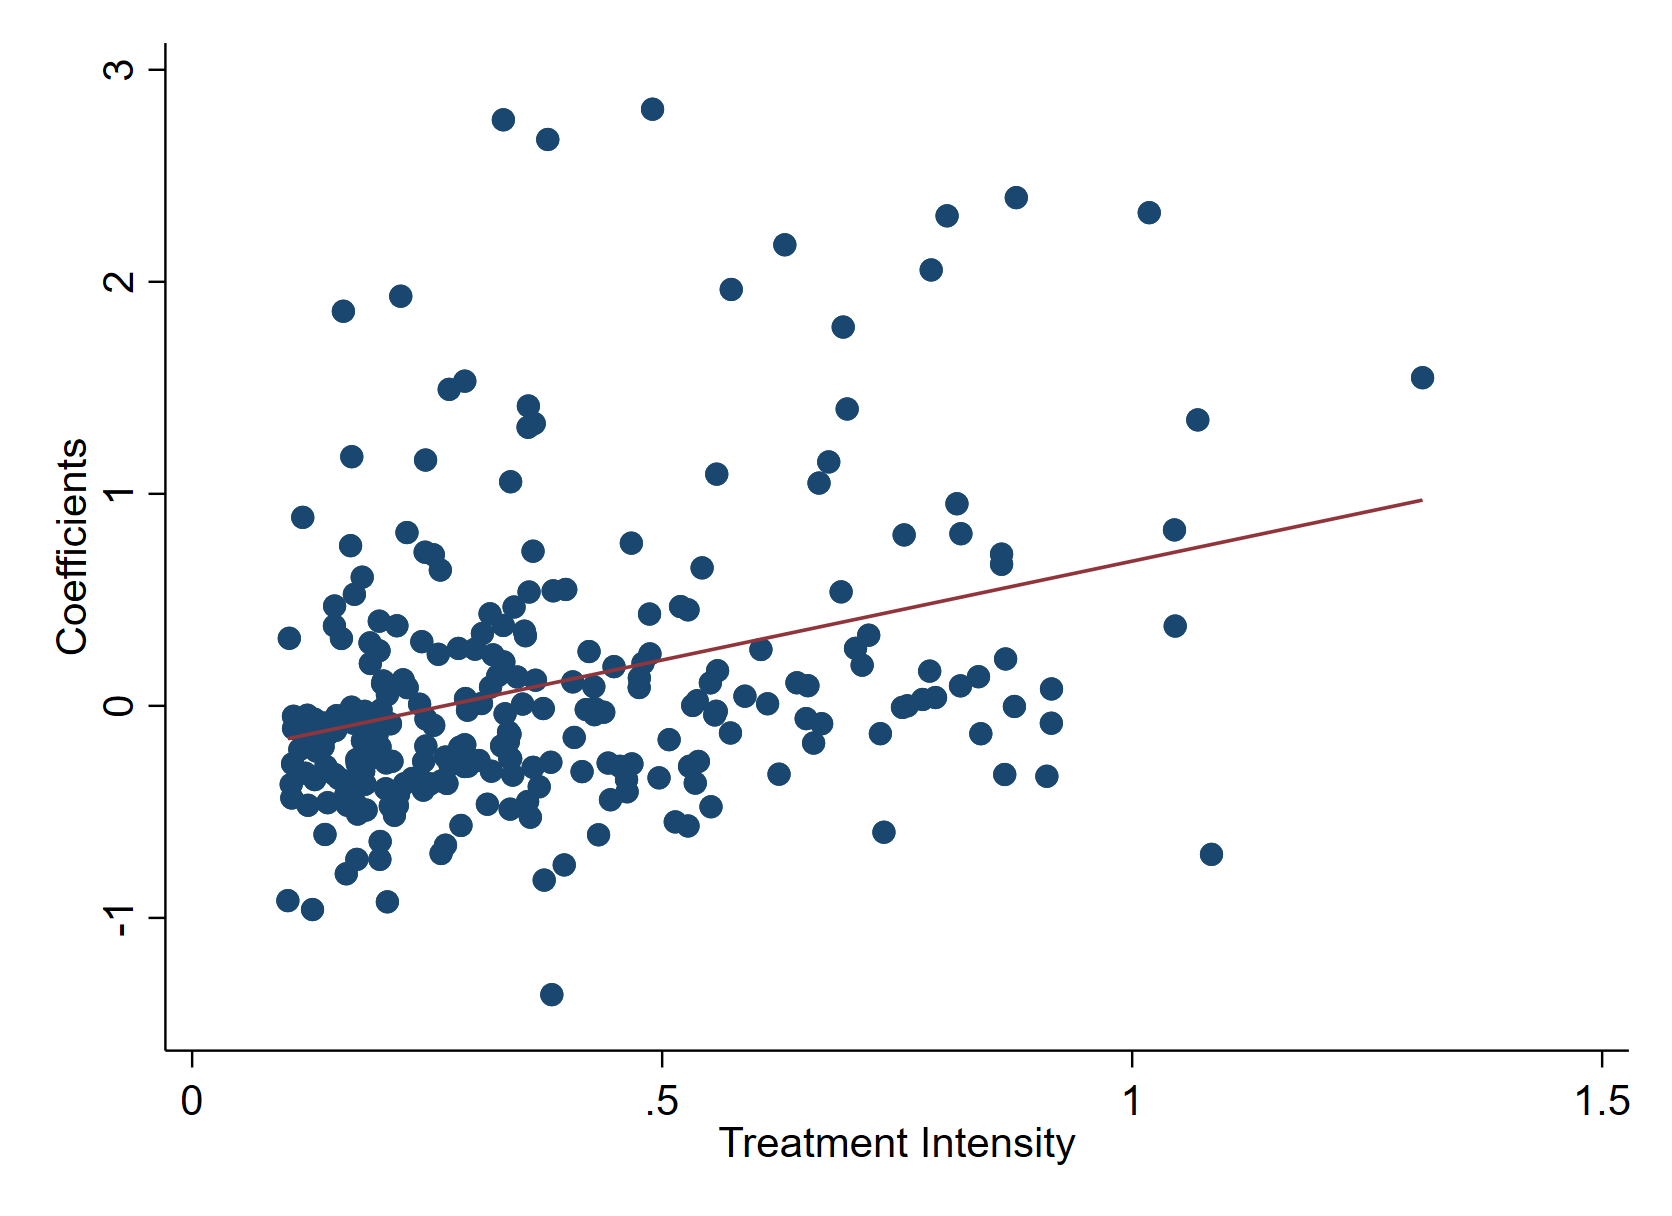
\includegraphics[width=\textwidth]{figures/appendix/pop_treatment_intensity_1990.png}
    \end{subfigure}
    \hfill
    \begin{subfigure}{0.48\textwidth}
        \centering
        \caption{2000}
        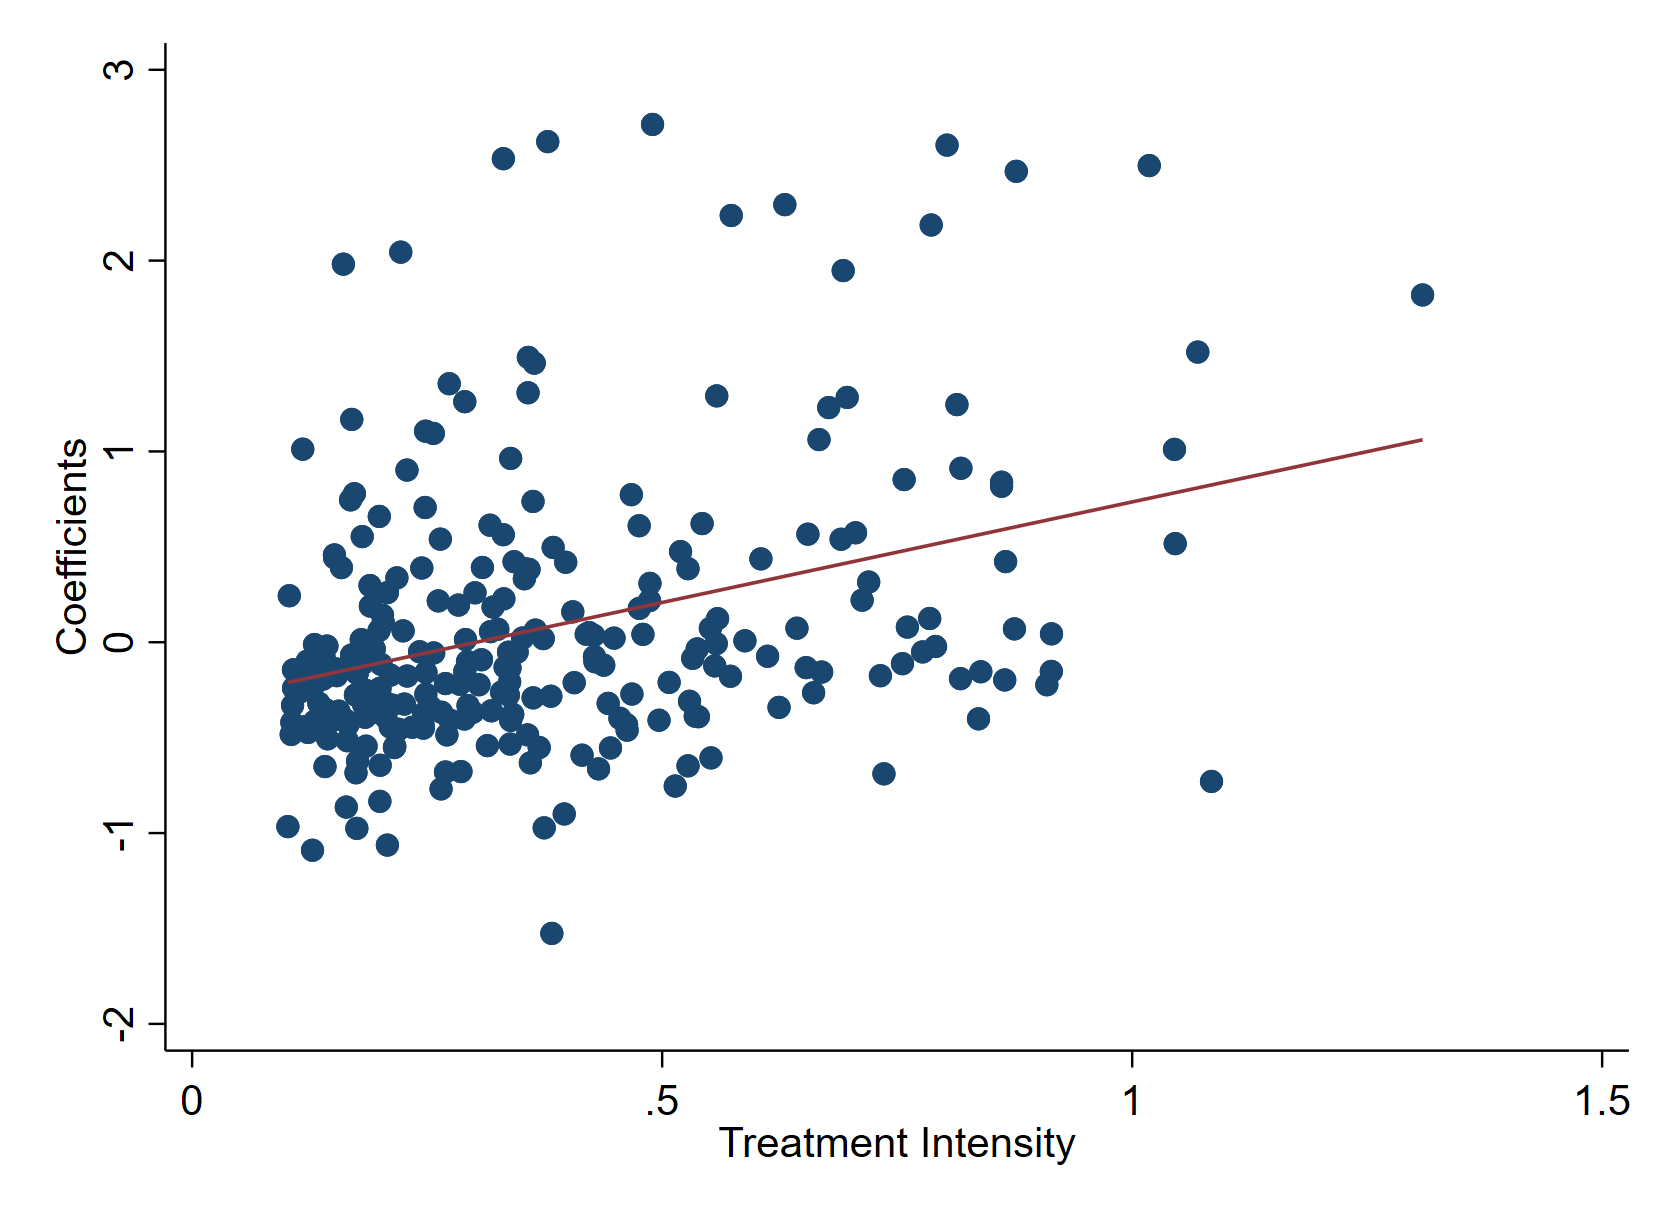
\includegraphics[width=\textwidth]{figures/appendix/pop_treatment_intensity_2000.png}
    \end{subfigure}
    \hfill
    \begin{subfigure}{0.48\textwidth}
        \centering
        \caption{2010}
        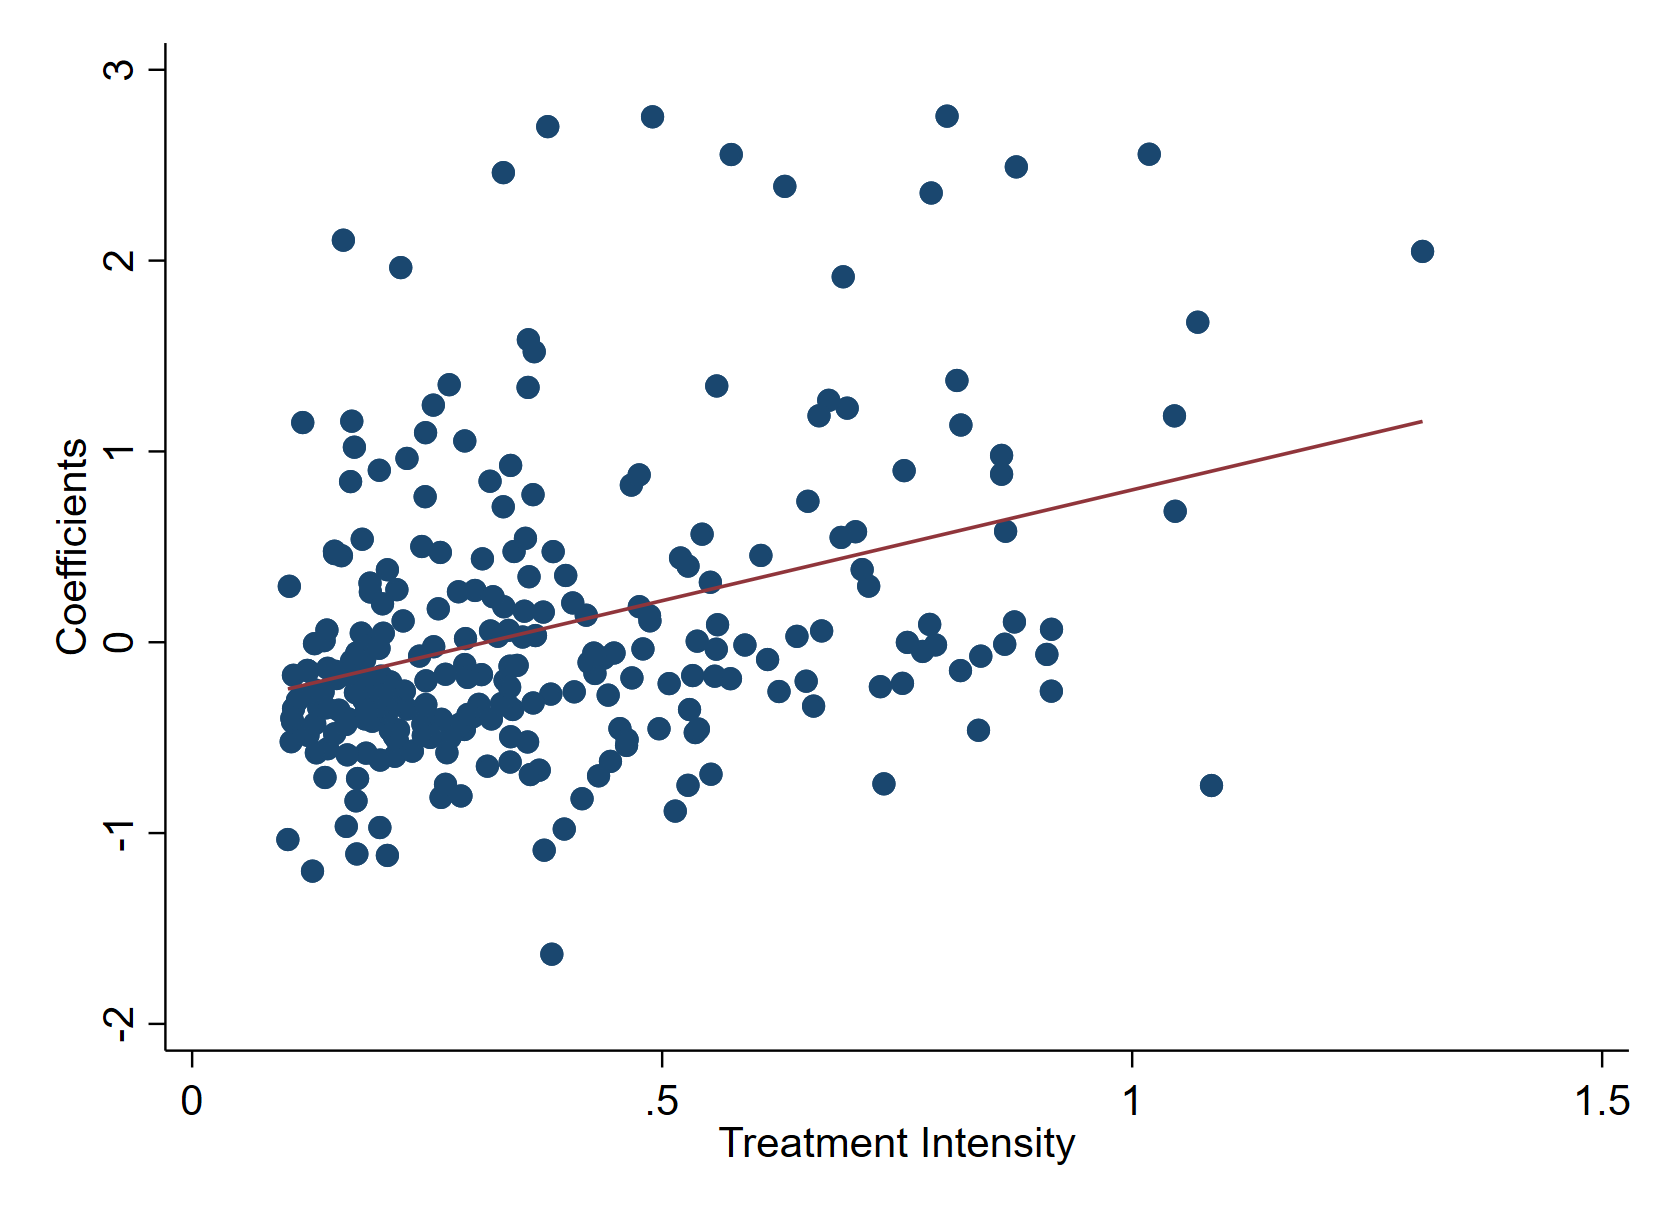
\includegraphics[width=\textwidth]{figures/appendix/pop_treatment_intensity_2010.png}
    \end{subfigure}
\end{figure}

\clearpage
\subsection{Additional Tables}
\suppressfloats[t]
\label{app:tables}

\begin{table}[htbp]\centering
\def\sym#1{\ifmmode^{#1}\else\(^{#1}\)\fi}
\caption{Event Study on Income and Population, 1970-2010}
\resizebox{\linewidth}{!}{
\begin{tabular}{l*{4}{c}}
\hline\hline
                    &\multicolumn{1}{c}{(1)}         &\multicolumn{1}{c}{(2)}         &\multicolumn{1}{c}{(3)}         &\multicolumn{1}{c}{(4)}         \\
                    &         GDP         &  Population         &Urban Population         &Urban Population Share         \\
\hline
1950.year $\times$ pin\_induced\_reduction&                     &      -0.188\sym{**} &      -0.019         &       0.169\sym{**} \\
                    &                     &     (0.076)         &     (0.085)         &     (0.069)         \\
1960.year $\times$ pin\_induced\_reduction&                     &      -0.193\sym{***}&       0.025         &       0.218\sym{***}\\
                    &                     &     (0.061)         &     (0.085)         &     (0.080)         \\
1970.year $\times$ pin\_induced\_reduction&       0.000         &       0.000         &       0.000         &       0.000         \\
                    &         (.)         &         (.)         &         (.)         &         (.)         \\
1975.year $\times$ pin\_induced\_reduction&       0.035         &                     &                     &                     \\
                    &     (0.057)         &                     &                     &                     \\
1980.year $\times$ pin\_induced\_reduction&       0.230\sym{***}&       0.154\sym{***}&       0.314\sym{***}&       0.159\sym{***}\\
                    &     (0.087)         &     (0.047)         &     (0.063)         &     (0.043)         \\
1985.year $\times$ pin\_induced\_reduction&       0.282\sym{***}&                     &                     &                     \\
                    &     (0.098)         &                     &                     &                     \\
1995.year $\times$ pin\_induced\_reduction&       0.400\sym{***}&                     &                     &                     \\
                    &     (0.116)         &                     &                     &                     \\
2000.year $\times$ pin\_induced\_reduction&       0.520\sym{***}&       0.265\sym{***}&       0.696\sym{***}&       0.431\sym{***}\\
                    &     (0.129)         &     (0.101)         &     (0.110)         &     (0.063)         \\
2005.year $\times$ pin\_induced\_reduction&       0.637\sym{***}&                     &                     &                     \\
                    &     (0.148)         &                     &                     &                     \\
2010.year $\times$ pin\_induced\_reduction&       0.650\sym{***}&       0.301\sym{***}&       0.786\sym{***}&       0.485\sym{***}\\
                    &     (0.145)         &     (0.112)         &     (0.122)         &     (0.070)         \\
1990.year $\times$ pin\_induced\_reduction&                     &       0.262\sym{***}&       0.580\sym{***}&       0.318\sym{***}\\
                    &                     &     (0.088)         &     (0.099)         &     (0.057)         \\
Observations        &        4248         &        3675         &        3675         &        3675         \\
\hline\hline
\end{tabular}}
\end{table}


\clearpage
\begin{table}[htbp]\centering
\def\sym#1{\ifmmode^{#1}\else\(^{#1}\)\fi}
\caption{Event Study on Agricultural Land Use, 1974-2010}
\begin{tabular}{l*{3}{c}}
\hline\hline
                    &\multicolumn{1}{c}{(1)}         &\multicolumn{1}{c}{(2)}         &\multicolumn{1}{c}{(3)}         \\
                    &   Sensitive         & Insensitive         &     Pasture         \\
\hline
1970.year $\times$ pin\_induced\_reduction&       0.000         &       0.000         &       0.000         \\
                    &         (.)         &         (.)         &         (.)         \\
1980.year $\times$ pin\_induced\_reduction&       0.313         &       0.240         &       0.365\sym{***}\\
                    &     (0.335)         &     (0.244)         &     (0.111)         \\
1990.year $\times$ pin\_induced\_reduction&       1.056\sym{**} &       0.223         &       0.369\sym{***}\\
                    &     (0.415)         &     (0.377)         &     (0.133)         \\
2000.year $\times$ pin\_induced\_reduction&       2.280\sym{***}&       1.008\sym{***}&       0.587\sym{***}\\
                    &     (0.531)         &     (0.362)         &     (0.170)         \\
2010.year $\times$ pin\_induced\_reduction&       2.172\sym{***}&       1.314\sym{***}&       0.490\sym{*}  \\
                    &     (0.623)         &     (0.414)         &     (0.273)         \\
Observations        &        2640         &        2640         &        2640         \\
\hline\hline
\end{tabular}
\end{table}


\end{document}